\subsection{Introduction}
\label{sec:PhysPerf_Introduction}

The detector performance specifications required by the physics programme of a future electron-positron Higgs factory 
operating at the $\PZ\PH$ production threshold and above, have been studied in the past for linear colliders. 
The different FCC-ee experimental environment, on the one hand, 
and the rich FCC-ee electroweak, QCD, and flavour physics programme offered by the very large event samples anticipated at the \PZ resonance 
(the so-called `Tera-\PZ' run), on the other, come with specific and entirely new challenges. 
The statistical uncertainties expected on key electroweak measurements,
both at the \PZ peak and at the $\PW\PW$ threshold, 
call for a superb control of the systematic uncertainties, 
and put commensurate demands on the acceptance, construction quality and stability of the detectors.
The specific discovery potential of feebly coupled particles in the huge FCC-ee event samples 
should also be kept in mind when designing the detectors. 

General considerations on the requirements for an FCC-ee detector were outlined in Refs.~\cite{Azzi:2021ylt, Blondel:2021ema}. 
In this section, a few benchmark analyses~\cite{SnowmassBenchmarkProcesses} are selected and their sensitivity dependence on various aspects of the detector performance are studied. 
In some cases, these studies result in a quantified performance requirement. 
It is understood that the extremely broad range of FCC-ee measurements has not yet been completely covered, and that some important requirements may be missing. 
The analyses performed for this report make use of the simulation of the performance of the detector concepts considered so far 
and described in Sections~\ref{sec:CLDDetCon} (CLD), \ref{sec:IDEADetCon} (IDEA), and~\ref{sec:ALLEGRODetCon} (ALLEGRO). 
For the reader's convenience, a brief account of these three concepts is given below, in Section~\ref{sec:PhysPerf_DetectorConcepts}; 
they are an important input to further optimisations and to the development of new concepts 
that might be better adapted to parts of the FCC-ee physics programme. 
As mentioned in Section~\ref{sec:overview}, FCC-ee will accommodate four interaction points. 
A single experiment may not be perfect in all aspects; 
a configuration with 4~IPs allows a range of detector solutions that will cover all physics opportunities.

Most of the studies reported here have been performed using computer-generated events processed through 
a fast detector simulation performed with the \textsc{Delphes} package. 
The chosen baseline is the IDEA detector~\cite{fcc-phys-cdr} described in Section~\ref{sec:IDEADetCon}. 
More details about the \textsc{Delphes} simulations used for the studies reported here can be found in Section~\ref{sec:delphes}.
To investigate the impact of the detector performance, variations around this detector baseline have been studied, 
either by smearing the reconstructed objects at the analysis level or by producing dedicated event samples. 
For some tracker-related studies, the performance expected with the CLD detector~\cite{Bacchetta:2019fmz} has also been looked at. 
The CLD main tracker consists of a set of layers of silicon sensors, in sharp contrast with the gaseous drift chamber of the IDEA detector. 
One study using a \textsc{Geant} simulation of the ALLEGRO noble-liquid calorimeter has also been made. 
A few preliminary performance studies or physics analyses have been performed using a full simulation of the CLD detector, 
as shown in Section~\ref{sec:PhysPerf_FullSim}.
After a brief overview of the detector benchmarks implemented in the simulations used for the studies reported here,
the following sections address, in turn, the requirements on the various subdetectors.

\subsection{Brief overview of the current detector concepts}
\label{sec:PhysPerf_DetectorConcepts}

Two detector concepts have been studied for FCC-ee at the time of the CDR: 
CLD, a consolidated option based on the detector design developed for CLIC, 
with a silicon tracker and a 3D-imaging highly-granular calorimeter; 
and IDEA, an innovative design developed specifically for FCC-ee, 
with a short-drift wire chamber and a dual-readout calorimeter. 
Since then, a third concept, ALLEGRO, has been proposed and is being developed, 
with an electromagnetic calorimeter based on a noble liquid. 
The three concepts considered so far have similar overall dimensions, 
with a length of 11--13\,m and a height of 10--12\,m. 
More details on these detector concepts are given in Section~\ref{sec:concepts}.

\subsubsection{The IDEA detector concept}

The tracking system of IDEA\footnote{Innovative Detector for an Electron-positron Accelerator.}
includes a silicon vertex detector (VXD) surrounded by a low mass drift chamber and an external layer of silicon micro-strip detectors. 
In the version used for the studies reported here, the VXD consists of 
a cylindrical `barrel' section made of five single layers of sensors, at radii between $R = 1.2$ and 31.5\,cm, 
and of two `endcap' sections (one on each side of the interaction point), each made of three disks of single layers of sensors. 
The drift chamber (DC) has a total length of 4\,m and consists of 112 layers of wires, placed at radii between 35 and 200\,cm. 
It allows `continuous tracking' and particle identification, as will be shown below. 
The total amount of DC material crossed by a particle emitted at 90$^{\circ}$ from the detector axis 
(defined by the bisector of the two beam axes) is 1.6\% of a radiation length. 
The DC is surrounded by a silicon wrapper that provides one precise spatial point at the end of the particle trajectory 
and measures the time-of-arrival of charged particles. 
The tracking system is immersed in a 2\,T magnetic field parallel to the detector axis, 
provided by a thin superconducting solenoid covering radii between 2.1 and 2.4\,m. 
Outside the tracker, a preshower made of $\mu$RWELL detectors and a dual-readout calorimeter of 2\,m depth and 7 interaction lengths, 
made of lead and fibres, measure the position and energy of electromagnetic and hadron showers. 
The dual-readout calorimeter (DRC) is sensitive to the independent signals from scintillation and Cerenkov light production, 
resulting in an excellent energy resolution for both electromagnetic and hadron showers.  
The simulations used here include a modification of the CDR calorimeter design, 
in which a 20\,cm deep (dual readout) electromagnetic calorimeter made of crystals is added upstream of the DRC, following Ref.~\cite{Lucchini:2020bac}. 
Finally, the muon system consists of layers of chambers based on $\mu$RWELL detectors embedded in the magnet return yoke. 

\subsubsection{The CLD detector concept}

The CLD\footnote{CLIC-Like Detector.}
detector has been adapted to the FCC-ee specificities from the CLIC detector model; 
it features a silicon pixel vertex detector and a silicon tracker, followed by a highly granular calorimeter. 
For the simulations used here, the barrel section of the VXD consists of three double-layers of sensors, at radii ranging between 1.2 and 5.8\,cm, 
and two endcap sections, consisting of three disks each, built as double-layer devices. 
The silicon tracker is made of six barrel layers, at radii from 12.7\,cm to 2.1\,m, and of two sets of eleven endcap disks. 
The material budget for the tracker modules is estimated to be 1.1--2.1\% of a radiation length per layer. 
The tracker is surrounded by a silicon-tungsten electromagnetic calorimeter (ECAL), which is 30\,cm or 22\,$X_0$ deep, 
and by a scintillator-steel hadron calorimeter (HCAL), that extends up to $R = 3.6$\,m; 
the combined ECAL plus HCAL thickness corresponds to 6.5 interaction lengths. 
The very high granularity of the calorimeter makes it particularly well suited for `particle flow' reconstruction techniques that, 
in CLD, are the key for reaching very good resolutions. 
A superconducting solenoid, delivering a 2\,T magnetic field, surrounds the calorimeter, at a radius of about 3.7\,m.  
The iron return yoke is instrumented with resistive plate chambers (RPC) that form the muon detection system. 
A detailed description of the CLD detector can be found in Ref.~\cite{Bacchetta:2019fmz}.

\subsubsection{The ALLEGRO detector concept}

The design of ALLEGRO\footnote{A Lepton-Lepton collider Experiment with Granular Read-Out.} 
is more recent than the IDEA and CLD designs. 
Its tracking system consists of a silicon vertex detector and a main tracker, which could either also be made of silicon sensors or be a gaseous detector. 
Surrounding the tracker is a high granularity noble-liquid ECAL, 
which could be made of lead (or tungsten) and liquid argon or, alternatively, of tungsten and liquid krypton. 
The magnet coil separates the ECAL from the high-granularity HCAL, 
which could be made of steel absorber plates interleaved with scintillator tiles, as envisaged for the CLD calorimeter. 
For the muon system, several options are under consideration.

\subsection{Measurement of the tracks of charged particles}
\label{sec:ch_part_tracking}

The detection of charged particles and the measurement of their momenta before they traverse a large amount of high density material 
is crucial for all physics analyses and for a successful particle-flow reconstruction~\cite{MLPF_NOTE}. 
This section deals with properties that are mostly related to the main tracker: 
the precise measurement of the track momentum and angles, and the reconstruction of highly-displaced vertices. 
The determination of the track impact parameters, which is largely provided by the vertex detector, is treated in Section~\ref{sec:PhysPerf:VXD}. 
The measurement of quantities related to the ionisation energy per unit length, useful to identify the nature of a charged particle, 
is covered in Section~\ref{sec:PhysPerf_PID}.

\subsubsection{Track momentum resolution: the measurement of the Higgs boson mass}
\label{sec:PhysPerf_HiggsRecoil}

The track momentum resolution is a key handle in many analyses. 
In particular, it directly impacts the reconstructed masses, which are often used to suppress backgrounds. 
Both IDEA and CLD tracker designs would offer an excellent track momentum resolution. 
For example, for 10\,GeV (50\,GeV) muons emitted at an angle of 90$^{\circ}$ with respect to the detector axis, 
the momentum resolution is about 0.5$\permil$ (1.5$\permil$) with the very light drift chamber of IDEA 
and about 2.5$\permil$ (3$\permil$) with the heavier full silicon tracker of CLD, 
the latter being dominated by the effect of multiple scattering. 
Some examples from B~physics, showing how the exceptional momentum resolution of the IDEA tracker separates the signals from the backgrounds, 
are presented in Sections~\ref{sec:PhysPerf_Bs2DsK} and~\ref{sec:PhysPerf_muons}.

In this section, the needs on the track momentum resolution are illustrated with the measurement of the Higgs boson mass, $m_{\PH}$,
which needs to be known to better than 4\,MeV (its intrinsic width), 
in view of a potential run at the Higgs resonance (Section~\ref{sec:eYukawa}).

This measurement, described in detail in Ref.~\cite{HiggsNoteRecoil}, exploits the Higgs-strahlung process, 
i.e., the associated production of a \PZ and a Higgs boson. 
Since, at a lepton collider, the total energy and momentum of the final state are well known, the mass of the system that recoils against the \PZ, 
called recoil mass and denoted $m_\text{recoil}$, 
can be reconstructed exclusively considering the \PZ decay products, irrespective of the Higgs boson decay. 
The $m_\text{recoil}$ distribution exhibits a sharp peak at $m_{\PH}$,
so that a fit to this distribution provides a precise measurement of the Higgs boson mass.  
Experimentally, the channel where the \PZ decays into a pair of muons offers the best resolution. 
A fit to the $m_\text{recoil}$ distribution for $\PZ(\PGm\PGm) \PH$ events at $\sqrt{s} = 240$\,GeV 
is displayed in the left panel of Fig.~\ref{fig:mH-recoil}, for various assumptions on the muon momentum resolution, 
while the right panel shows the result of a likelihood fit of the distribution of signal events in the presence of background, with the same assumptions. 
Even with a perfect measurement of the momentum of the muons, 
the width of the $m_\text{recoil}$ peak would be limited by the beam energy spread (BES), 
which amounts\footnote{The beam energy spread values used for the studies reported here are taken from Ref.~\cite{talk_IS_workshop_december}.} 
to 0.185\% of the beam energy at $\sqrt{s} = 240$\,GeV, 
so that $m_{\PH}$ would be determined with an uncertainty of 3.95\,MeV 
(including the contribution of other sub-dominant systematic uncertainties~\cite{HiggsNoteRecoil}), 
for an integrated luminosity of 10.8\,ab$^{-1}$.

\begin{figure}[ht]
\centering
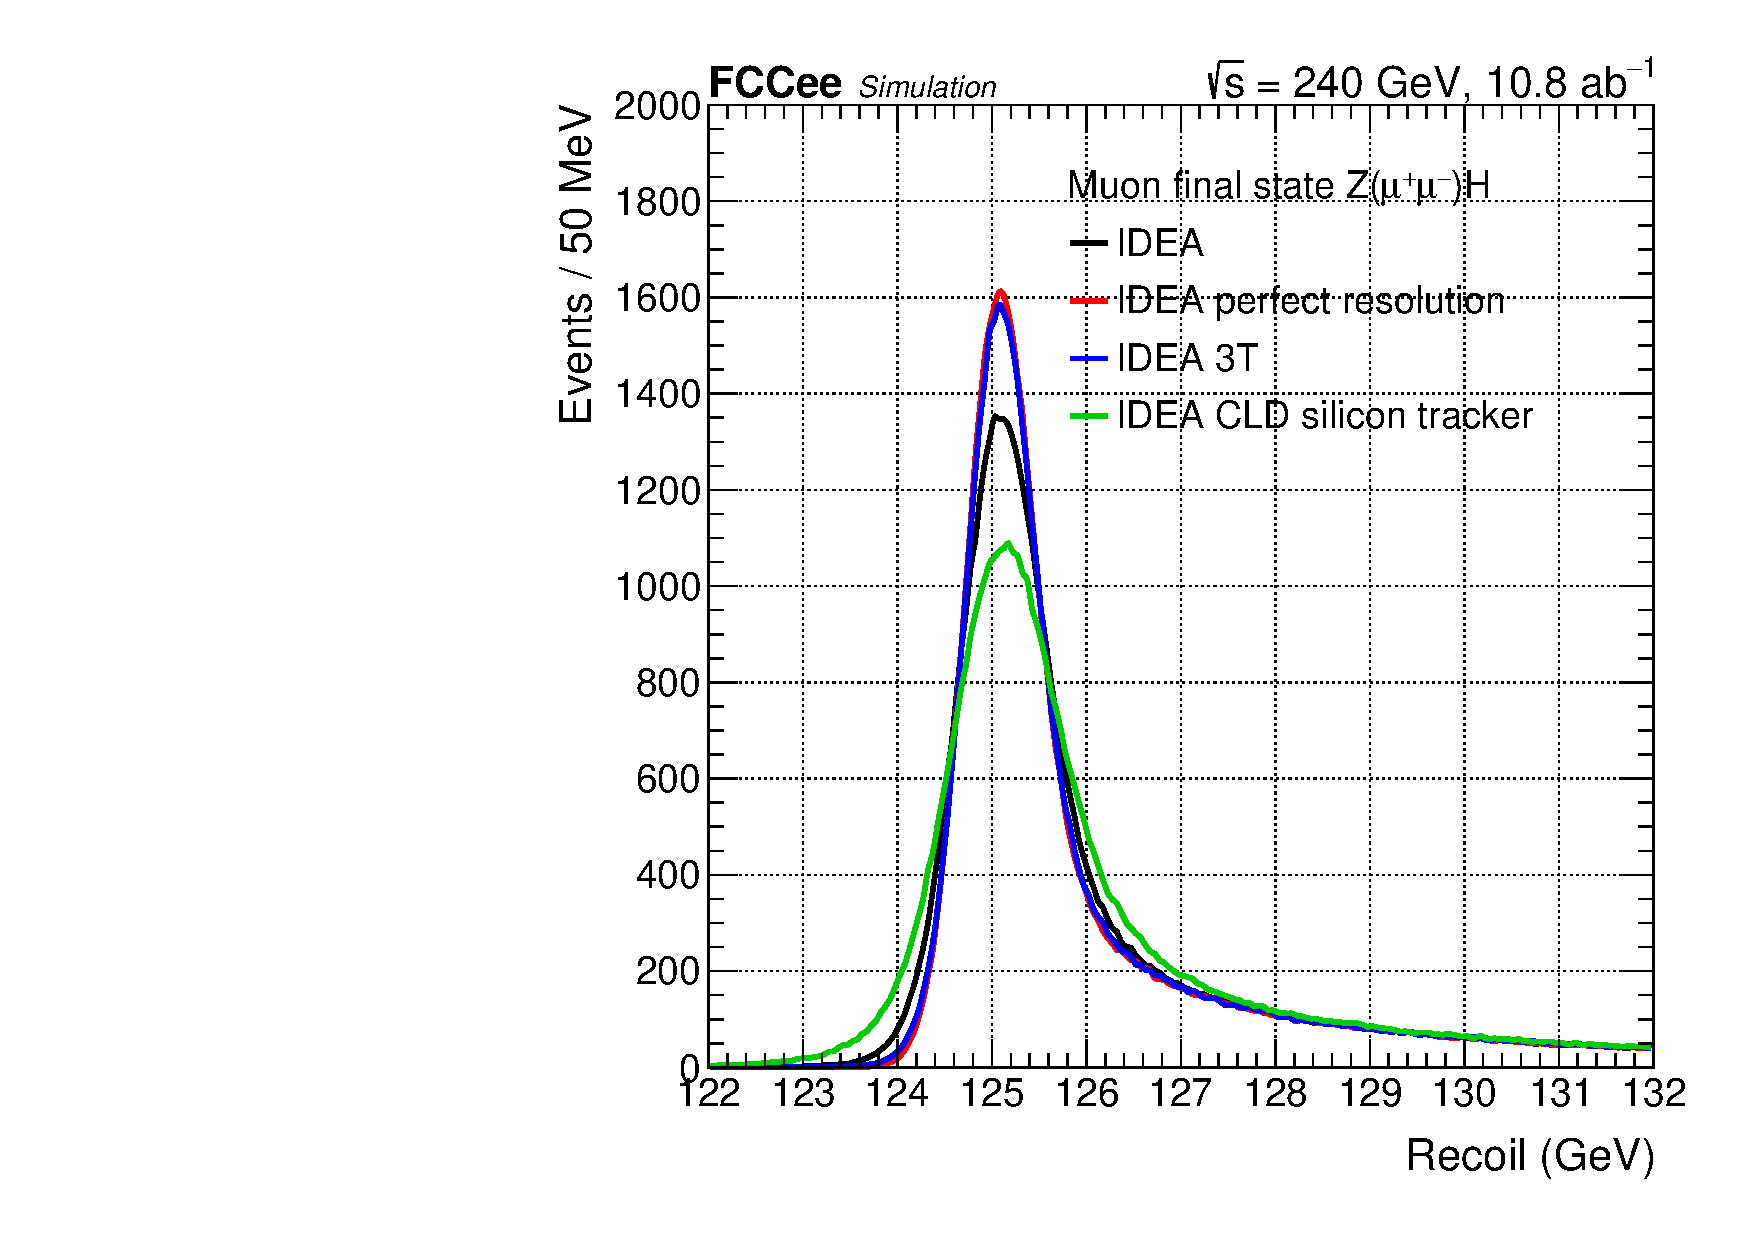
\includegraphics[width=0.48\textwidth]{DetectorRequirements/Figs/HiggsRecoil_IDEA_IDEAL_2T_3T_CLD_mumu_mrec.pdf}
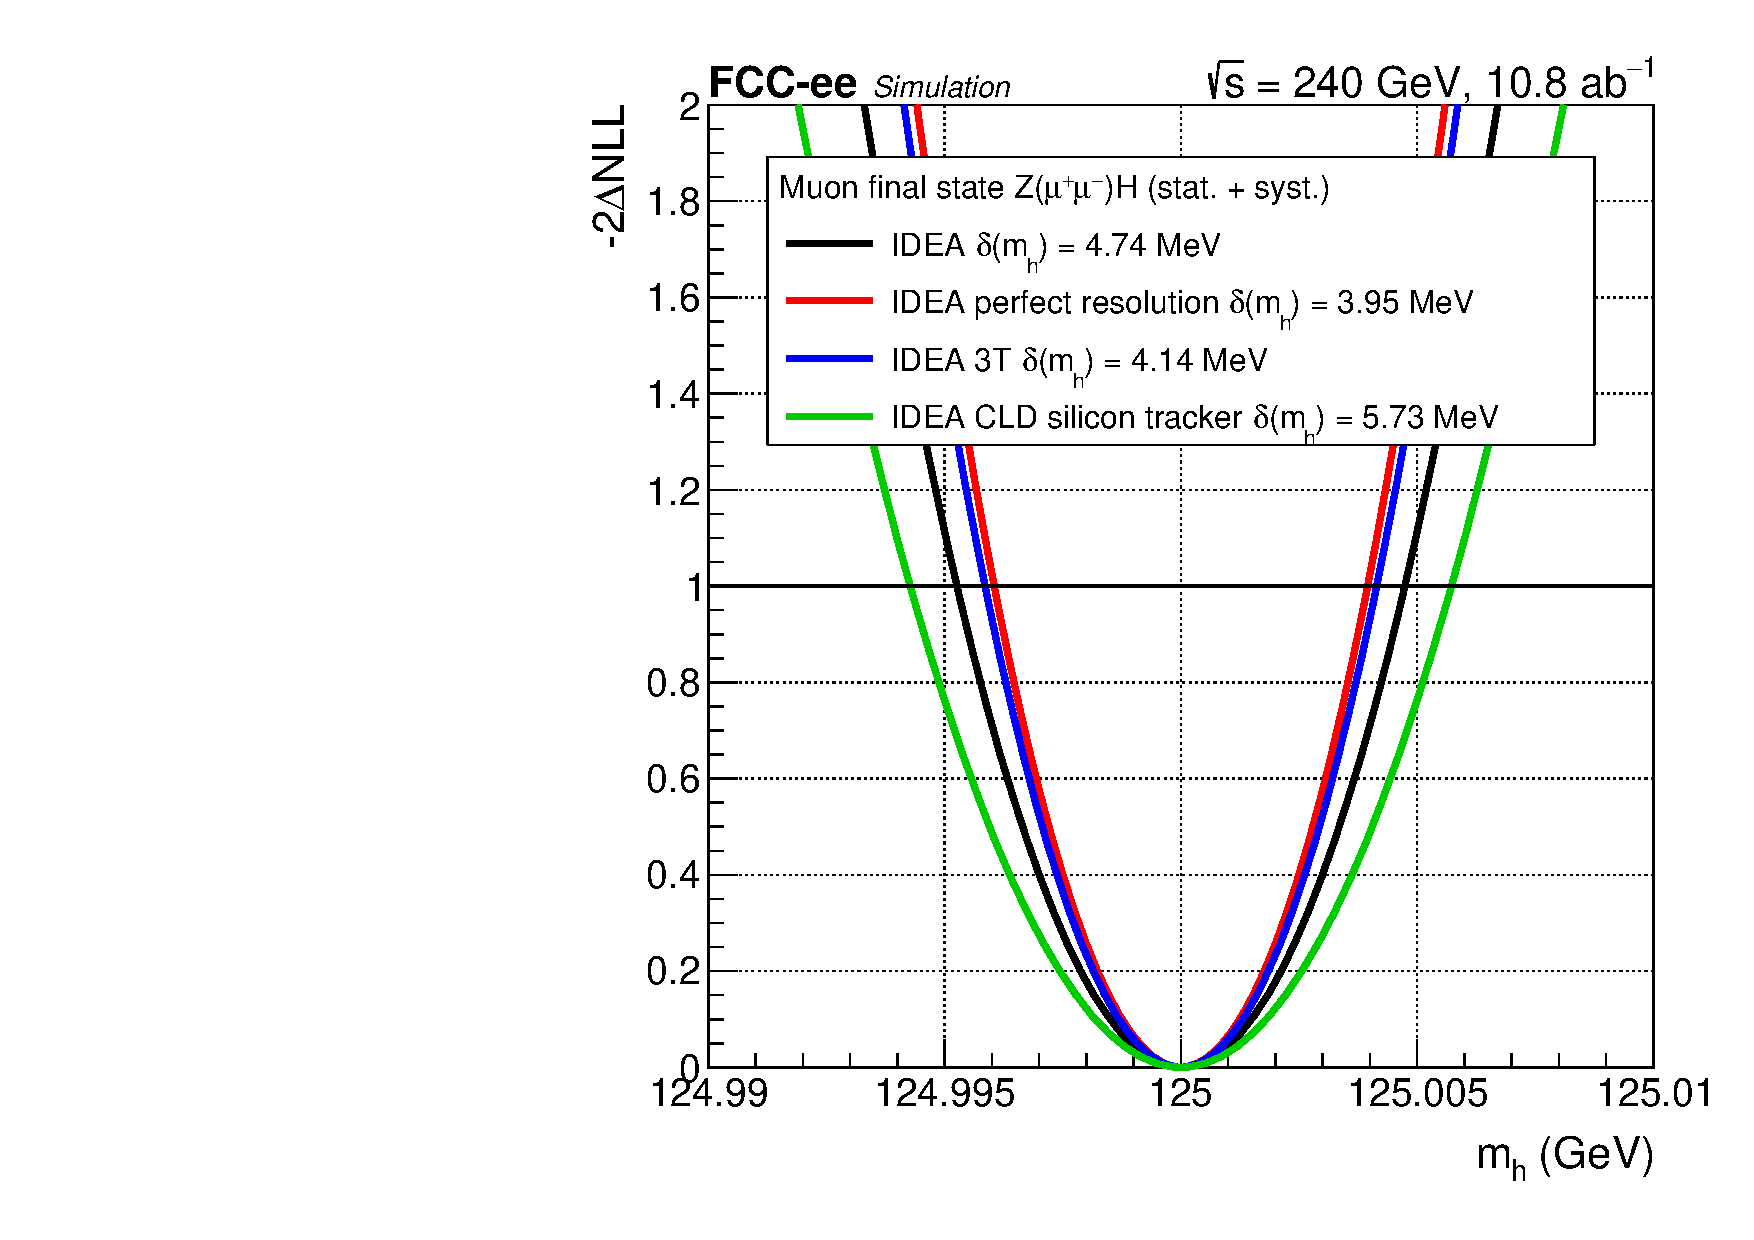
\includegraphics[width=0.48\textwidth]{DetectorRequirements/Figs/HiggsRecoil_IDEA_IDEAL_2T_3T_CLD_mumu.pdf}
\caption{Left: Fits to the distribution of the Higgs boson recoil mass in $\PZ\PH$ events, where the \PZ decays into muons, 
assuming an ideal momentum resolution (red), such that the resolution on the recoil mass is determined by the beam energy spread, 
or the momentum resolution of the IDEA (black and blue) or CLD (green) detectors. 
The blue curve corresponds to a 3\,T magnetic field, instead of the 2\,T field used for the other distributions. 
Right: Corresponding Higgs boson mass measurements.}
\label{fig:mH-recoil}
\end{figure}

The decay muons, with typical momentum of ${\cal{O}}(50)$\,GeV, should be measured with a momentum resolution better than the BES,
so that the mass resolution be not limited by the momentum 
measurement\footnote{Having a momentum resolution for ${\cal{O}}(50)$\,GeV muons better than or comparable to the BES is also an important requirement in the search for $\PZ \to \PGt\PGm$ lepton flavour violating decays, at $\sqrt{s} = 91$\,GeV. The analysis strategy requires a clear tau decay in one hemisphere and a beam-energy muon in the other, 
in order to suppress the $\PZ \to \PGt\PGt$ background~\cite{Dam:2018rfz}.}. 
This goal is achieved with the IDEA detector (black curves in Fig.~\ref{fig:mH-recoil}), only considering the muon decay channel. 
The full silicon tracker of CLD, in its current implementation, performs less well (green curves) because of the larger amount of material, 
which leads to increased multiple scattering, the factor that dominates the muon momentum resolution, even for the relatively high momentum range of interest. 
However, the goal of 4\,MeV on the measured Higgs boson mass would most likely be achieved by combining the muon and electron decay channels 
(Section~\ref{sec:PhysPerf_ECAL}). 
The blue curves in Fig.~\ref{fig:mH-recoil} show what would be expected, with the IDEA tracker, 
if the detector magnetic field were increased 
from 2 to 3\,T\footnote{For the highest luminosity runs at the \PZ peak, %and at the $\PW\PW$ threshold, 
the magnetic field of the detector is constrained to not exceed about 2\,T, as explained in Section~\ref{sec:mdi}. 
At $\sqrt{s} = 240$\,GeV, the blow-up of the beam emittance that results from a higher magnetic field is negligible 
and running, for example, with a 3\,T field, which would provide a better track momentum resolution, is not ruled out.}; 
the result is a 33\% improvement of the momentum resolution and a 14\% improvement on the total mass uncertainty.

\subsubsection{Track momentum resolution: the \texorpdfstring{\PZ}{Z} width and the stability of the momentum scale}

The point-to-point uncertainty on the centre-of-mass energy in the scan of the \PZ lineshape is, 
together with the knowledge of the BES and the point-to-point uncertainty on the integrated luminosity, 
a dominant source of systematic uncertainty in the \PZ width measurement. 
The reconstructed peak position of the dimuon invariant mass distribution in $\epem \to \PGmp\PGmm$ events provides a measurement of the centre-of-mass energy. 
As proposed in Ref.~\cite{Blondel:2019jmp} and developed in Ref.~\cite{perez_2024_gyqhp-m0480}, 
the aforementioned uncertainty can be assessed from the difference in this reconstructed peak position between the energy points used in the lineshape scan. 
More details about the method are given in Section~\ref{sec:EPOL_input_from_the_experiments}. 
Figure~\ref{fig:ptp-sqrt-uncertainty} shows the statistical uncertainty with which the peak position is expected to be determined 
at $\sqrt{s} = 87.9$, 91.2, and 94.3\,GeV, with the full FCC-ee event sample. 
With the track momentum resolution provided by the IDEA tracker, this precision reaches 20\,keV for the two off-peak energies, 
such that the difference in the collision energy at these two points can be measured with an uncertainty of about 28\,keV, 
leading to an 11\,keV uncertainty on the extracted \PZ width. 
With the resolution offered by the CLD tracker, this difference is measured with two times larger uncertainty, 
resulting in an uncertainty of 22\,keV in the \PZ width.

\begin{figure}[t]
\centering
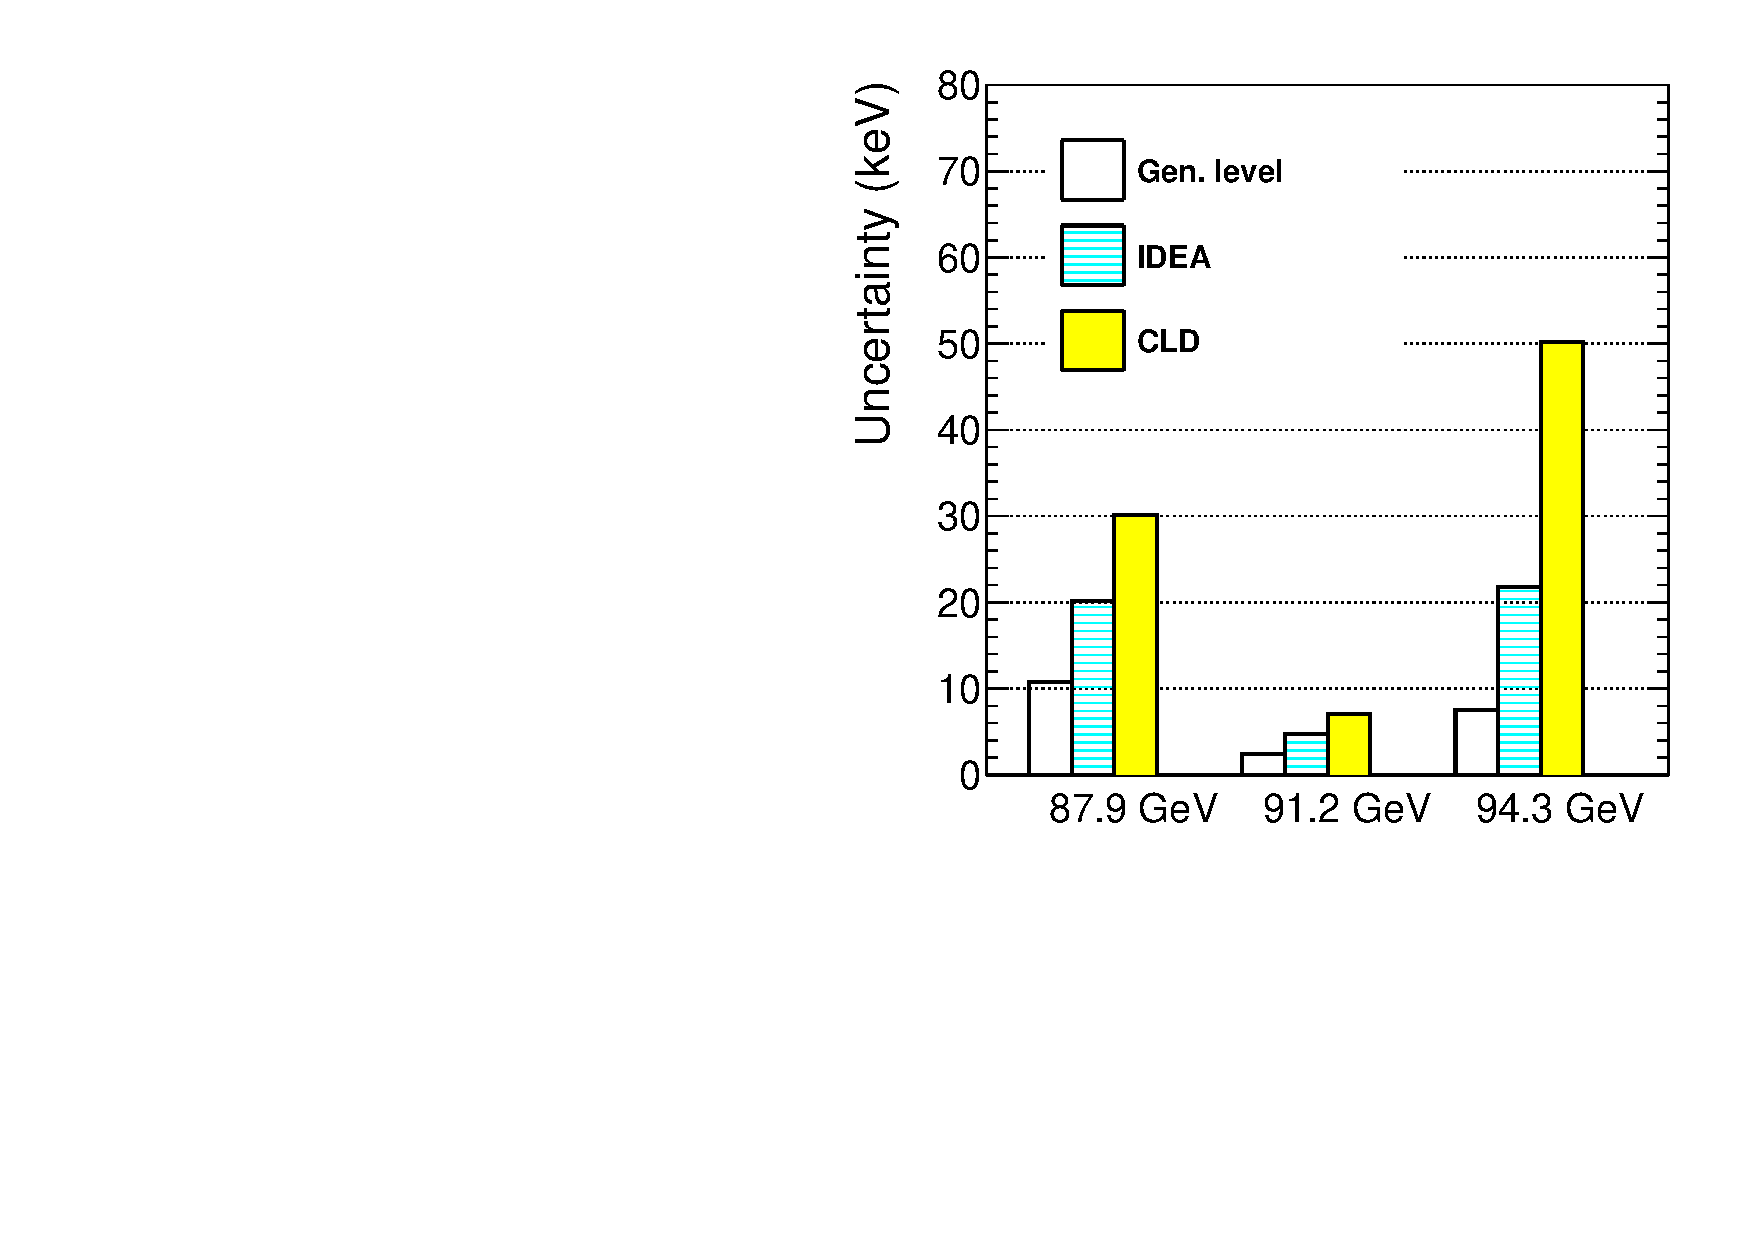
\includegraphics[width=0.4\textwidth]{Physics/DetectorRequirements/Figs/summary_Zwidth_sqrts_uncertainty.pdf} 
\caption{Statistical uncertainty in the peak position of the measured dimuon invariant mass distribution, 
expected with the full FCC-ee event sample of the \PZ lineshape scan 
(125\,ab$^{-1}$ at the \PZ peak and 40\,ab$^{-1}$ at each off-peak energy). 
This uncertainty is shown assuming an ideal detector resolution (leftmost bars), 
the resolution of the IDEA tracker (middle bars), 
and that of the CLD tracker (rightmost bars).}
\label{fig:ptp-sqrt-uncertainty}
\end{figure}

Such a precision, however, requires that the scale of the momentum measurements 
(and, in particular, of the magnetic field) 
be stable at the level of a few $10^{-7}$ (20\,keV over $\sqrt{s}$, to ensure a 20\,keV uncertainty on the peak position) 
or, at least, that its variations be monitored at that level. 
A monitoring at this level of precision may be difficult to achieve with magnetic NMR probes. 
However, the large samples of well-known resonances, 
in particular of \PKS decaying into $\PGpp\PGpm$, provide an in-situ monitoring at this exceptional precision. 
An efficient and high purity algorithm that reconstructs $\PKS \to \PGpp\PGpm$ decays is presented below. 
It allows a \PKS to be reconstructed in about every second \PZ event, when the \PZ decays hadronically. 
With a mass resolution better than 400\,keV with the IDEA detector, 
the position of the \PKS mass peak can be determined with a relative uncertainty of $2.3 \times 10^{-9}$ 
with an integrated luminosity of 40\,ab$^{-1}$ at $\sqrt{s} = 87.9$\,GeV 
(and even better at $\sqrt{s} = 94.3$\,GeV, given the larger cross section). 
This dataset could, hence, be split into, e.g., 100 subsamples in time, 
and the \PKS resonance be reconstructed in 100 bins, 
to ensure monitoring of the scale stability at the required level of $2.3 \times 10^{-7}$.

\subsubsection{Angular resolutions}
\label{sec:PhysPerf_TrackAngles}

The polar and azimuthal angles of the momentum of a prompt charged particle, at its production vertex, 
are given by the angles of the corresponding track at its distance of closest approach to the detector axis.
The angular resolutions in the two detector concepts considered so far vary between 
about 20\,$\mu$rad for high momentum particles produced in the central region of the detector and a few mrad for soft forward particles~\cite{Bacchetta:2019fmz, softwareNote}. 
The contribution of these angular resolutions to the uncertainty in the recoil mass shown above is negligible compared to that of the momentum resolution. 
For the reconstruction of the mass of heavy-flavoured hadrons, 
the momenta of the daughter particles must be taken at the decay vertex of the hadron 
and the resolution of the azimuthal angle crucially relies on the reconstruction of this decay vertex (see Section~\ref{sec:PhysPerf:VXD}). 
Nevertheless, for all examples considered involving \PB mesons 
(see, e.g.,\ Sections~\ref{sec:PhysPerf_Bs2DsK} and~\ref{sec:PhysPerf_muons}), 
the mass resolution remains completely dominated by the momentum resolution.

A precise determination of the polar and azimuthal angles is crucial for exploiting the over-constrained kinematics of many processes in $\epem$ collisions. 
That is the case, in particular, of muon pair production.
As shown in Ref.~\cite{Blondel:2019jmp}, for $\epem \to \PGmp\PGmm (\PGg)$ dimuon events, 
the crossing angle and the longitudinal momentum imbalance can be reconstructed event-by-event from the sole measurement of the polar and azimuthal angles of both muons. 
The BES, which is a crucial ingredient in the extraction of the \PZ width at Tera-\PZ, 
can then be derived from the width of the longitudinal momentum imbalance distribution. 
To ensure that the BES uncertainty has a negligible effect on the extracted \PZ width, 
muon tracks from \PZ decays must be measured with an  angular resolution of 0.1\,mrad or better, 
a requirement fulfilled~\cite{Bacchetta:2019fmz, softwareNote} by the detector concepts presented in the CDR. 
Moreover, the mean of the longitudinal momentum imbalance distribution provides the longitudinal boost. 
Its determination constrains the energy losses of the beams in their separate rings~\cite{note_EPOL} and, consequently, 
has a crucial influence on the precision of the \PZ and \PW mass measurements.

Another example that exploits the angles of dimuon events is the determination of the centre-of-mass energy well above the $\PW\PW$ threshold, 
where the resonant depolarisation method cannot be applied. 
In particular, at $\sqrt{s} = 240$\,GeV, the centre-of-mass energy needs to be determined to ${\cal{O}}$(1)\,MeV 
in order not to spoil the Higgs boson mass determination from the recoil mass. 
The over-constrained kinematics of radiative return events $\epem \to \PZ (\PGg)$ with $\PZ \to \PGmp\PGmm$ 
(accompanied by an initial-state radiated photon along the direction of one of the beams) 
allows the determination of $\sqrt{s}$ from the precise knowledge of the $\PZ$ mass and the muon angles alone. 
The target precision for the $\sqrt{s}$ measurement may set tighter requirements on the angular resolutions than those given above.

\subsubsection{Number of tracker layers and highly-displaced vertices}
\label{sec:PhysPerf_Kshorts}

The reconstruction of long-lived particles (LLPs) that decay into charged particles within the tracker volume 
after having crossed the innermost layers of the vertex detector requires that the main tracker be able to efficiently identify such highly-displaced vertices. 
Typical use cases are the searches for LLPs predicted in many models that extend the Standard Model 
(Section~\ref{sec:PhysicsCaseBSM} and Refs.~\cite{note_HNL_Polesello_Valle_mujj,note_LLPs_ExoticHiggsDecays})
or the reconstruction of decays that involve \PKS or \PGL hadrons.

As an example, the case of \PKS mesons produced in $\PBp \to \PKp \PDz$ decays, followed by the decay of the \PDz meson into a $\PKS \PGpz$ pair, is considered here. 
The reconstruction of the $\PKS \to \PGpp \PGpm$ decay is detailed in Ref.~\cite{Aleksan:2021fbx}. 
The \PKS candidates are built from pairs of opposite-charge particle tracks that do not come from the primary vertex and that can be fitted to a common vertex, 
with a reconstructed mass close to the nominal \PKS mass. 

\begin{figure}[ht]
\centering
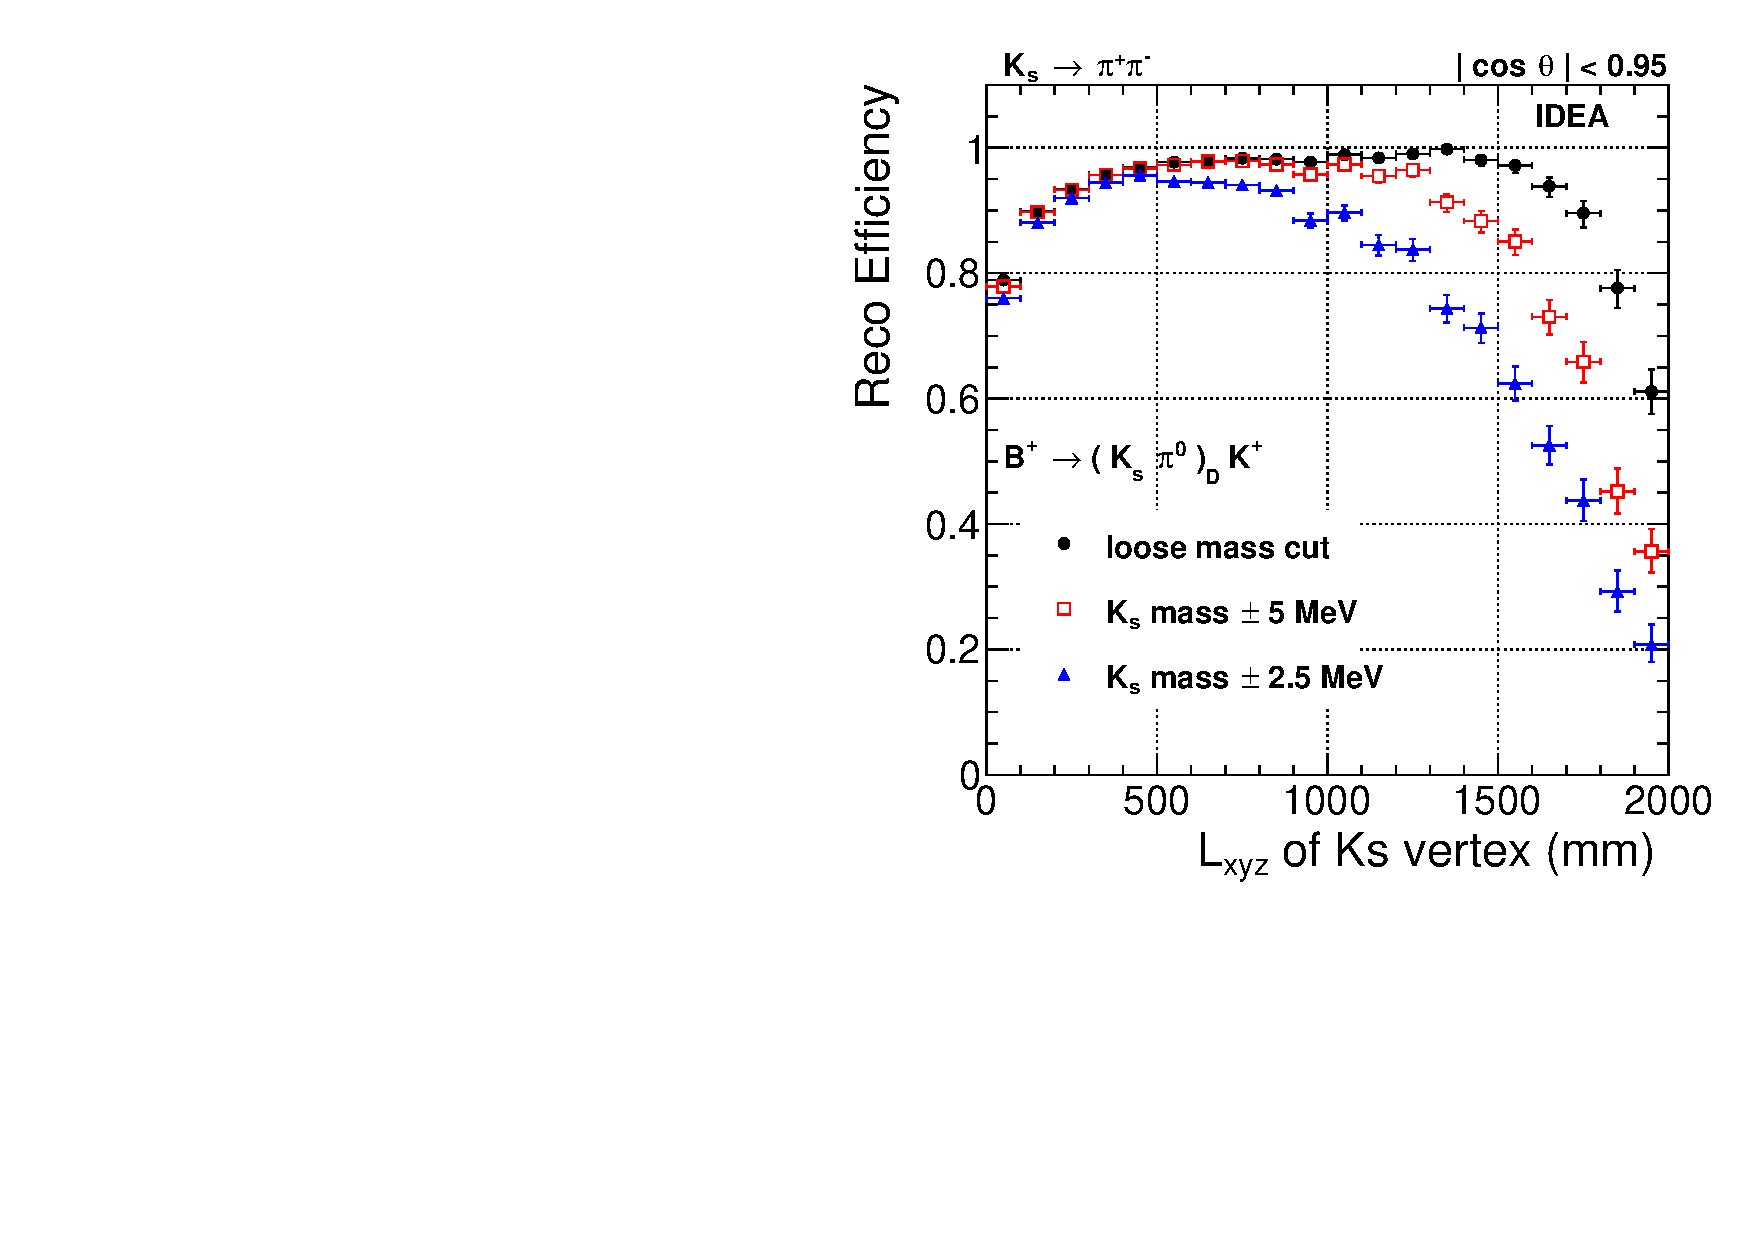
\includegraphics[width=0.48\textwidth]{DetectorRequirements/Figs/Ks_efficiency_IDEA.pdf}
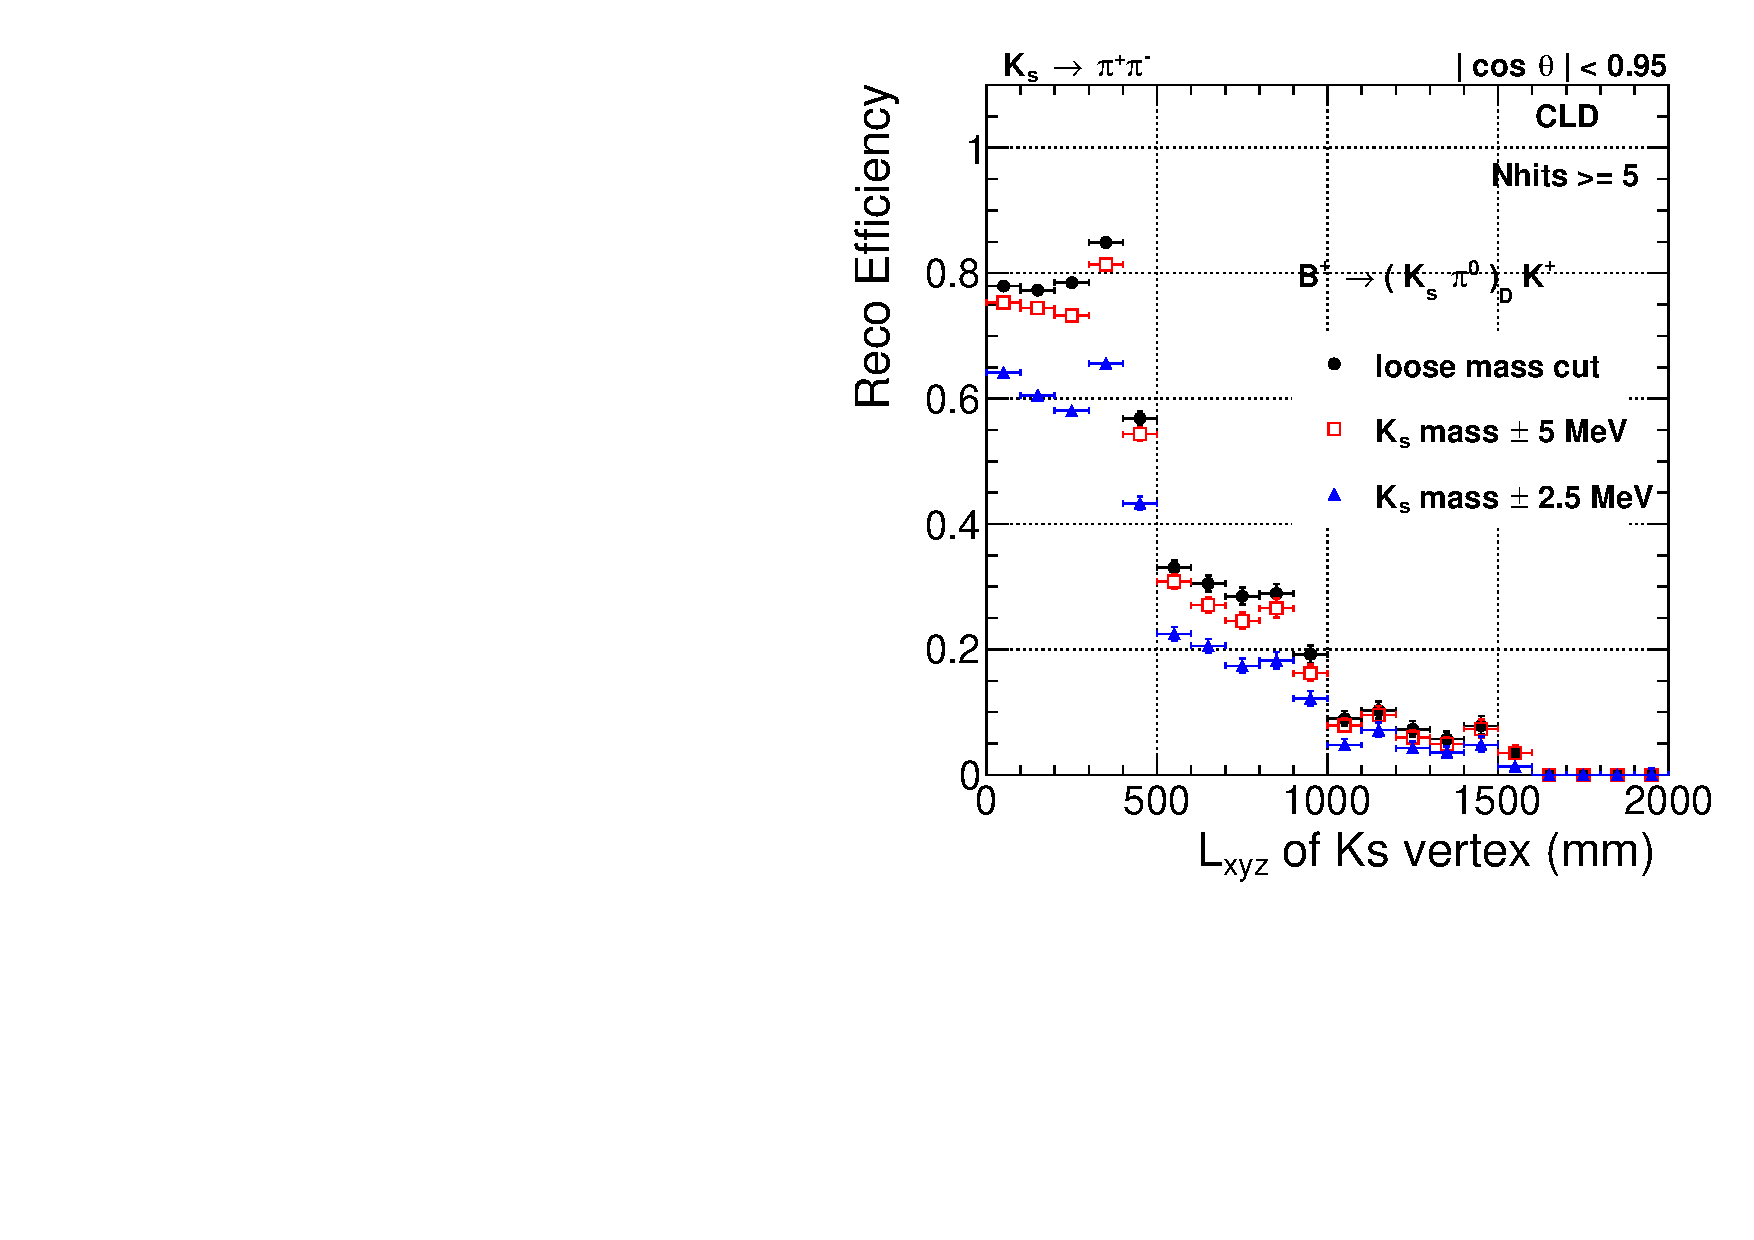
\includegraphics[width=0.48\textwidth]{DetectorRequirements/Figs/effi_CLD_5hits.pdf}
\caption{The \PKS reconstruction efficiency for kaons emitted in $\PBp \to (\PKS \PGpz)_{\PD} \, \PKp$ decays,
as a function of the distance $L_{xyz}$ between the \PKS decay vertex and the interaction point, 
for several thresholds on the \PKS mass candidate, for the IDEA (left) and CLD (right) detector concepts.}
\label{fig:Ksreco_efficiency}
\end{figure}

The \PKS reconstruction efficiency obtained with the IDEA detector is shown in Fig.~\ref{fig:Ksreco_efficiency}~(left), 
as a function of the distance between the \PKS decay vertex and the interaction point, $L_{xyz}$. 
The efficiency is defined for the \PKS mesons that come from $\PBp \to (\PKS \PGpz)_{\PD} \, \PKp$ decays 
for which the daughter pions satisfy the acceptance requirement $|\cos \theta| < 0.95$. 
Within a mass window of $\pm 5$\,MeV, the efficiency remains higher than 80\%, as long as the \PKS meson decays within 1.5\,m from the interaction 
point\footnote{The drop in efficiency observed at small flight distances is due to the correlation of the flight distance with the \PKS momentum: 
the pion tracks from \PKS mesons that decay close to the IP are softer and more affected by multiple scattering or may lead to curling tracks (`loopers').}.
At larger distances, the efficiency drops because the pion tracks only traverse a small fraction of the tracker. 
The right panel of Fig.~\ref{fig:Ksreco_efficiency} shows the corresponding efficiency for events processed through a \textsc{Delphes} simulation of the CLD detector. 
As expected, the performance is much worse than that of IDEA. 
Steps corresponding to the positions of the tracker layers are clearly visible. 
For example, since there are only four barrel layers at a radial distance larger than 40\,cm, 
the efficiency for selecting 5-hit tracks displaced by more than 40\,cm vanishes in the central region, explaining the first step seen in the figure. 
Also, the \PKS mesons that decay within a few tens of centimetres from the IP have a lower detection efficiency than that of the IDEA drift chamber, 
given the larger amount of material of the full silicon tracker and the correspondingly larger multiple scattering and worse resolutions on the \PKS reconstructed vertex and mass. 

While some optimisations could be made to the full silicon tracker considered here, 
it is clear that an efficient reconstruction of $\PKS \to \PGpp \PGpm$ decays and, more generally, 
of long-lived particles that lead to late appearing tracks 
calls for a highly transparent tracker, a large tracking volume, and a considerable number of measurement layers. 

\subsubsection{Work ahead}

\paragraph{Tracker acceptance and efficiencies}
The search for the $\PB \to \PK^{*}\, \PGt \PGt$ rare decay, described in more detail in Section~\ref{sec:DetReq_vertex}, sets requirements on the track efficiencies. 
Demanding that both taus decay into three prongs is particularly useful for this analysis and leads to a final state with six soft pion tracks. 
A momentum acceptance down to 100--150\,MeV is necessary to maintain a good signal efficiency. 
With a magnetic field of 2\,T, the requirement of a minimum number of, e.g., 5~hits to reconstruct a track,
implies that there be at least five measurement layers at a radius smaller than 33\,cm (50\,cm) to reconstruct a track with a transverse momentum of 100\,MeV (150\,MeV). 
This requirement on the position of the layers of the vertex detector and of the innermost layers of the main tracker 
is fulfilled by both the IDEA and the CLD tracker designs~\cite{softwareNote, Bacchetta:2019fmz}. 
As an illustration, the tracking efficiency as a function of transverse momentum is shown in Fig.~\ref{fig:mltracking}~(left), 
for tracks reconstructed with a novel machine-learning algorithm, discussed in Section~\ref{sec:PhysPerf_FullSim}. 
In addition, the track reconstruction efficiency as a function of the distance to the closest charged hadron in a jet is shown in Fig.~\ref{fig:mltracking}~(right). 
It indicates that CLD features a slightly larger efficiency in dense hadronic environments, 
possibly due to a better separation capability of two close-by tracks, driven by the superior single-point spatial resolution provided by silicon sensors.

\begin{figure}[ht]
\centering
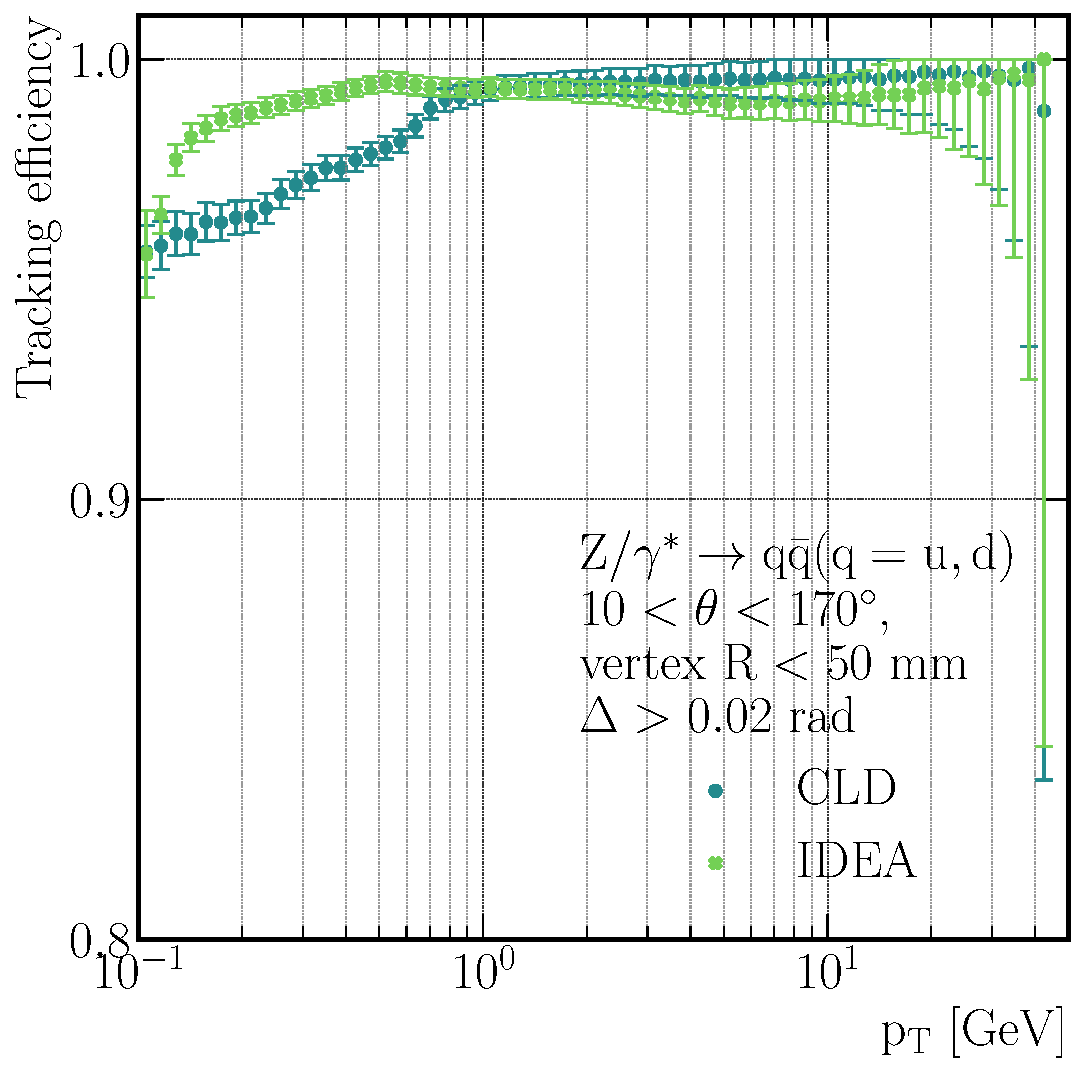
\includegraphics[width=0.465\textwidth]{Physics/DetectorRequirements/Figs/Tracking_efficiency_vs_pt_comparison_IDEA_CLD_Zjj.pdf} 
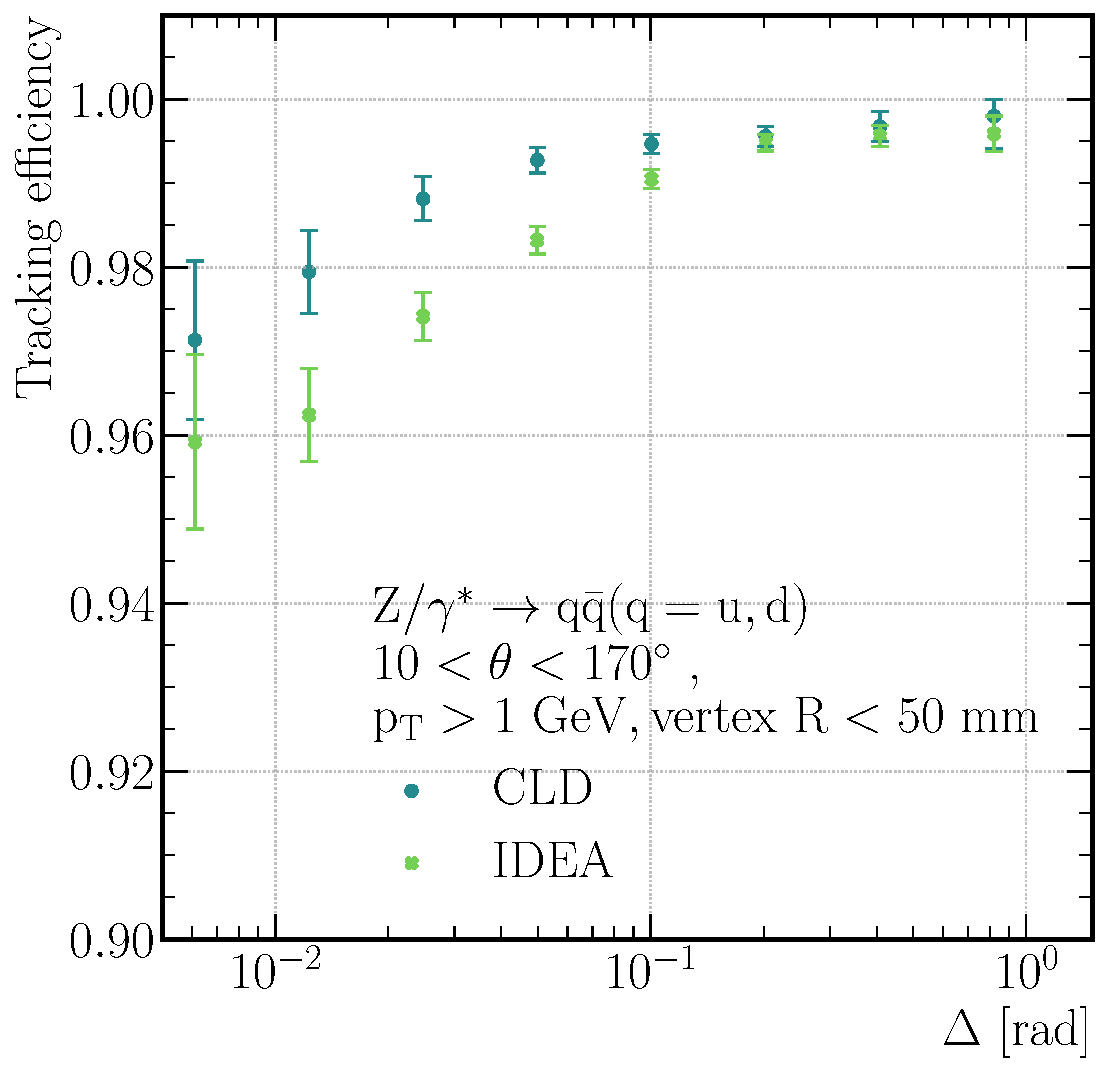
\includegraphics[width=0.475\textwidth]{Physics/DetectorRequirements/Figs/Tracking_efficiency_comparison_IDEA_CLD_Zjj.pdf}
\caption{Tracking efficiency evaluated with full simulation of the CLD and IDEA detectors using the ML-based approaches, 
as a function of \pt (left) and of the angle $\Delta_\text{MC}$ to the closest generated charged particle (right).}
\label{fig:mltracking}
\end{figure}

The measurement of the luminosity from $\epem \to \PGg \PGg$ events (Section~\ref{sec:PhysPerf_ECAL}), to a precision of about $10^{-5}$, 
requires a very precise knowledge of the large background from $\epem \to \epem$ events. 
The targeted precision will set a requirement on the $\Pe / \PGg$ separation that, in turn, 
will constrain the tracker inefficiency and the precision with which this inefficiency is known. 
In addition, the ratio of the partial width of the \PZ boson decay into hadrons to that into muons, $R_{\PGm}$, 
will be measured with a statistical precision of about $5 \times 10^{-6}$ at Tera-\PZ. 
Counting the number of $\PGmp\PGmm$ events with a similar level of systematic uncertainty 
sets a very challenging requirement on the knowledge of the tracking (and muon chamber) efficiency.   

\paragraph{Track angles}
The angular resolutions provided by the current tracker designs comply, with a good safety margin, with the requirements set by the studies done so far, as shown above. 
Further studies are needed to check if other measurements set tighter requirements. 
Beside the measurement of $\sqrt{s}$ from the radiative return events previously mentioned, 
methods that are being developed to precisely determine dilepton acceptance in-situ (Section~\ref{sec:PhysPerf_gammagamma}) may call for better angular resolutions. 

\subsubsection{Preliminary conclusions}

The performance of a gaseous tracker and of a full silicon tracker have been shown and quantified with several examples. 
\begin{itemize}
\item Having a large number of measurement points along the tracks, as offered by a gaseous tracker, 
is crucial for an efficient reconstruction of \PKS and $\Lambda$ hadrons or other long-lived particles that decay into charged particles, 
and is a clear bonus for an experiment with a strong focus on flavour or BSM physics.
\item The momentum resolution offered by both designs looks adequate for Higgs boson measurements. 
This statement probably holds as well for most electroweak measurements, with the notable exception of the \PZ width measurement. 
For flavour physics at the \PZ peak, where low momentum tracks are involved, 
a low mass gaseous tracker is advantageous since the momentum resolution is minimally affected by multiple scattering.
\item The tracker volume, extending to a radius of about 2\,m, 
may have to be reduced a little in order to free some space to accommodate a detector dedicated to charged-hadron particle identification 
(which may be needed in particular for the CLD option, see Section~\ref{sec:PhysPerf_PID}). 
A reduction by ${\cal{O}}$(20)\,cm would degrade the momentum resolution by about 15\%, 
as shown in Section~\ref{sec:Detectors_MainTracking}.
This effect might be partly compensated by reducing the amount of material in the CLD tracker layers. 
\end{itemize}

\subsection{Requirements for the vertex detector}
\label{sec:PhysPerf:VXD}

The measurement of the track impact parameters is driven by the performance of the vertex detector, 
as it provides very precise spatial points in the tracker layers closest to the beams. 
A precise measurement of these parameters is crucial for reconstructing vertices, 
for efficient identification of heavy quarks and of taus, 
and for accurate lifetime measurements. 
The resolution on these parameters typically scales as
\begin{equation}
\sigma( d_0 ) = a \oplus \frac{b}{p \sin^{3/2} \theta} \, ,
\label{eq:track_impact_parameter}
\end{equation}
where the asymptotic term, $a$, is driven by the single hit resolution, 
while the second term represents the contribution of multiple scattering and depends on the material of the vertex detector layers and of the beam pipe. 
The radial distance of the first layer of the vertex detector is also crucial~\cite{Bedeschi:2022rnj}. 
In the simulations used for the studies reported here, the radius of the beam pipe is 1\,cm, 
that of the innermost layer of the vertex detector is 1.2\,cm, 
and the material crossed by a particle emitted at a polar angle $\theta$ before the first VXD measurement corresponds to $0.67 \% \, / \, \sin \theta$ of a radiation length.

\subsubsection{Heavy-flavour tagging and the Higgs boson coupling to charm quarks}
\label{sec:PhysPerf_Hcc}

Previous flavour tagging studies made for linear colliders~\cite{Behnke:2013lya,Linssen:2012hp} colliders 
concluded that $a \approx 5$\,$\mu$m and $b \approx 15$\,$\mu$m/GeV 
(in Eq.~\ref{eq:track_impact_parameter}) 
are adequate for measuring the Higgs boson couplings to bottom and charm quarks. 
These requirements have been revisited in the context of the present study. 
In particular, major progress has been made in recent years in the field of flavour tagging algorithms. 
Machine-learning approaches, on one hand, and the ever increasing computing power, on the other, 
have significantly improved the performance of flavour tagging with respect to that of the algorithms that were the state-of-the-art a decade ago, 
so that more ambitious goals can be contemplated today. 
The algorithm developed for the studies reported here is based on {\textsc{ParticleNet}}~\cite{Qu:2019gqs} 
and uses state-of-the-art jet representations and an advanced graph neural network architecture. 
This algorithm is referred to as {\textsc{ParticleNetIDEA}} and is described in more detail in Ref.~\cite{Bedeschi:2022rnj}. 
With this new tool, an efficient and pure identification of jets induced by gluons or even strange quarks (see Section~\ref{sec:PhysPerf_strangeTagging}) 
is available and the tagging efficiency of bottom and charm quarks is much larger than what was achieved with the previous generation of algorithms, 
for the same purity.

This algorithm is a key ingredient in the measurement of the Higgs boson couplings to bottom, charm, and strange quarks, as well as to gluons, 
as described in detail in Ref.~\cite{note_Higgs_to_hadrons}. 
The analysis exploits the $\PZ\PH$ events at $\sqrt{s} = 240$\,GeV and considers the channels where the \PZ boson decays 
to pairs of muons or electrons, to jets, or to neutrinos, the latter channel currently providing the best sensitivity. 
The probabilities that each jet originates from a bottom, charm, or strange quark, or from a gluon, 
are determined by the \textsc{ParticleNetIDEA} algorithm and are used to categorise events into orthogonal categories, 
each enriched in one of the different Higgs boson decay modes and depleted in the others. 

The branching ratios of the Higgs boson decays to $\PQb\PAQb$, $\PQc\PAQc$, $\PQs\PAQs$, and $\Pg\Pg$ pairs
are measured in all categories with a simultaneous fit to the recoil mass distributions 
(and, for the $\PZ \to \PGn \PAGn$ channel, to the visible mass distributions).

The anticipated precision of the coupling measurements is summarised in Section~\ref{sec:PhysicsCaseHiggsEW}. 
With an integrated luminosity of 10.8\,ab$^{-1}$, the $\PH \to \PQb\PAQb$ and $\PH \to \PQc\PAQc$ event yields 
(cross section times branching ratio) 
can be measured with a precision of 0.21\% and 1.66\%, respectively.

The dependence of this precision on alternative beam pipe and vertex detector configurations 
has been studied and compared to the sensitivity obtained with the baseline IDEA detector design. 
Beam pipes with twice or half the nominal material budget have been studied. 
A vertex detector with the barrel layers shifted by 0.5\,cm towards larger radii 
and an option where the heavier beam pipe is complemented by a single-point resolution degraded by a factor of~2 
have also been considered. 
The measurement of the $\PH \to \PQc\PAQc$ and $\PH \to \PQb\PAQb$ branching fractions is marginally improved or degraded for the assumed better or worse scenarios. 
A transverse impact parameter resolution of \mbox{2--3}\,$\mu$m is achieved with the baseline IDEA vertex detector. 
A resolution worsened by a factor of~2 remains largely sufficient to identify displaced tracks 
originating from boosted \PD and \PB meson decays produced in $\PH \to \PQb\PAQb$ and $\PQc \PAQc$ decays 
and has, therefore, a small impact on the expected precision. 
A comprehensive discussion on the impact of vertex detector assumptions on the tagging performance can be found in Ref.\cite{sciandra_2024_gt813-z8602}.

\subsubsection{Reconstruction of vertices and the measurement of the 
\texorpdfstring{$\PB \to \PK^* \PGt\PGt$}{B to K* tau tau} branching fraction}
\label{sec:DetReq_vertex}

With the current version of the IDEA detector, the primary vertex, for example in events where a \PZ decays to hadrons, 
is typically reconstructed with a resolution of 2--3\,$\mu$m in the $x$ and $z$ coordinates, 
and of a few tens of nm in the $y$ direction 
(driven by the r.m.s.\ of the beam position in the vertical direction, 
as shown in Table~\ref{tab:IR_parameters}, Section~\ref{sec:mdi}), 
using a beamspot constraint in the vertex fit. 
For displaced vertices, the resolution depends very much on the track multiplicity of the vertex, on the track momenta and angles, and on the angular separation of the tracks. 
In the various \PB-physics processes that have been looked into so far, 
the resolution on the 3D distance between the interaction point and the displaced vertex typically varies between $\sim$\,10 and $\sim$\,80$\mu$m. 
For example, in the $\PBs \to \PDs \PK$ decay, where the \PDs decays to $\PK\PK\PGp$, 
the resolution of 15\,$\mu$m obtained on the \PBs decay vertex is sufficient for time-dependent CP violation measurements, 
since it is ${\cal{O}}$(40) times smaller than the distance travelled by the \PBs during one oscillation period. 

However, some processes of interest for flavour physics impose very strong demands on the reconstruction of vertices.
So far, the most stringent requirements on the performance of the vertex detector come from the measurement of the branching ratio of the, 
yet unobserved, $\PB \to \PK^* \PGt\PGt$ decay.  
This branching fraction is predicted to be very small in the Standard Model, at the level of ${\cal{O}}(10^{-7})$, 
and the current experimental upper limit is larger than this prediction by three orders of magnitude. 
New physics contributions can potentially result in a significant enhancement of this branching fraction. 
Consequently, its measurement is an important goal of the FCC-ee physics programme. 
A detailed analysis of the feasibility of this measurement at the \PZ pole is reported in Ref.~\cite{miralles_2024_9t6w9-mmd12}, and is summarised below. 

\begin{figure}[ht]
\centering
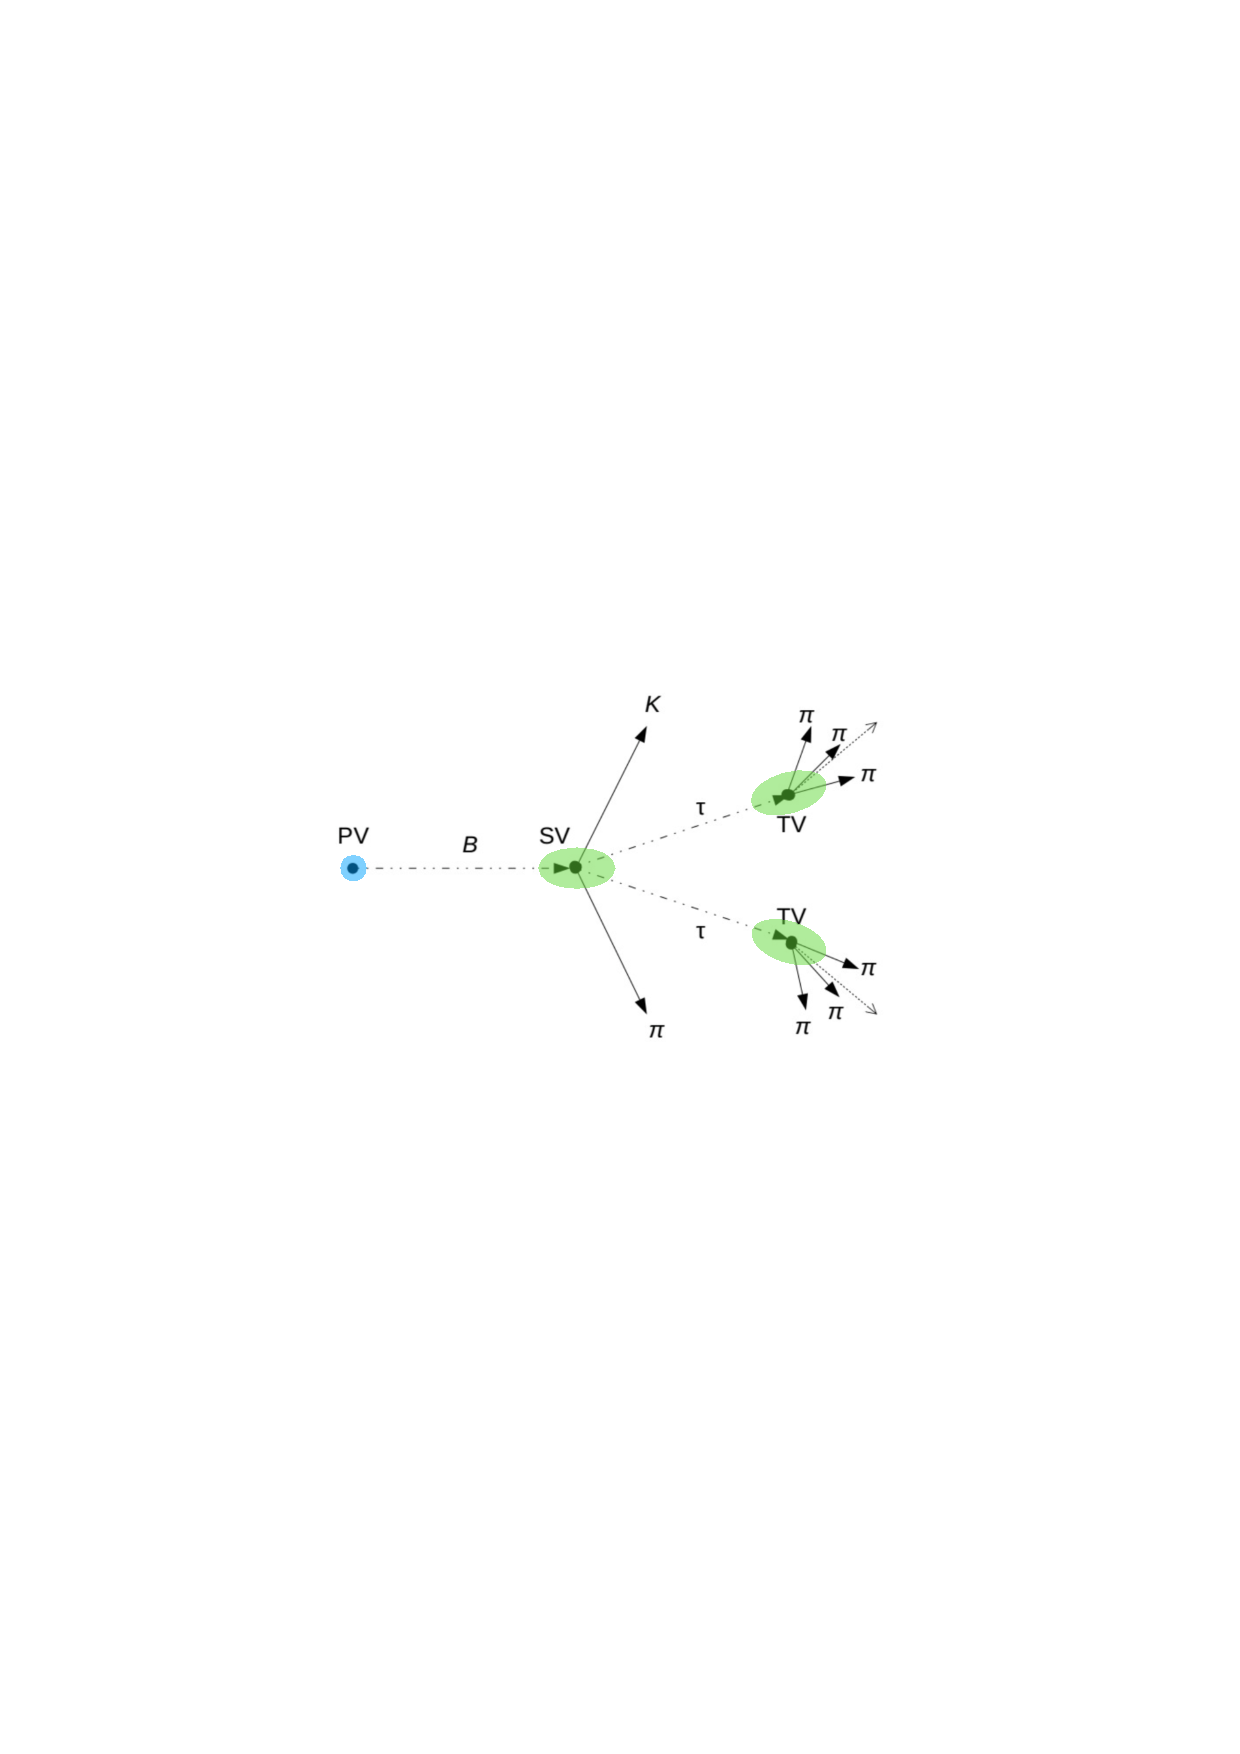
\includegraphics[width=0.5\textwidth]{DetectorRequirements/Figs/KstarTauTau_decay_chain.pdf} 
\caption{Decay chain under study for a measurement of the $\PB \to \PK^* \PGt\PGt$ branching fraction.}
\label{fig:KstarTauTau_decaychain}
\end{figure}
\begin{figure}[ht]
\centering
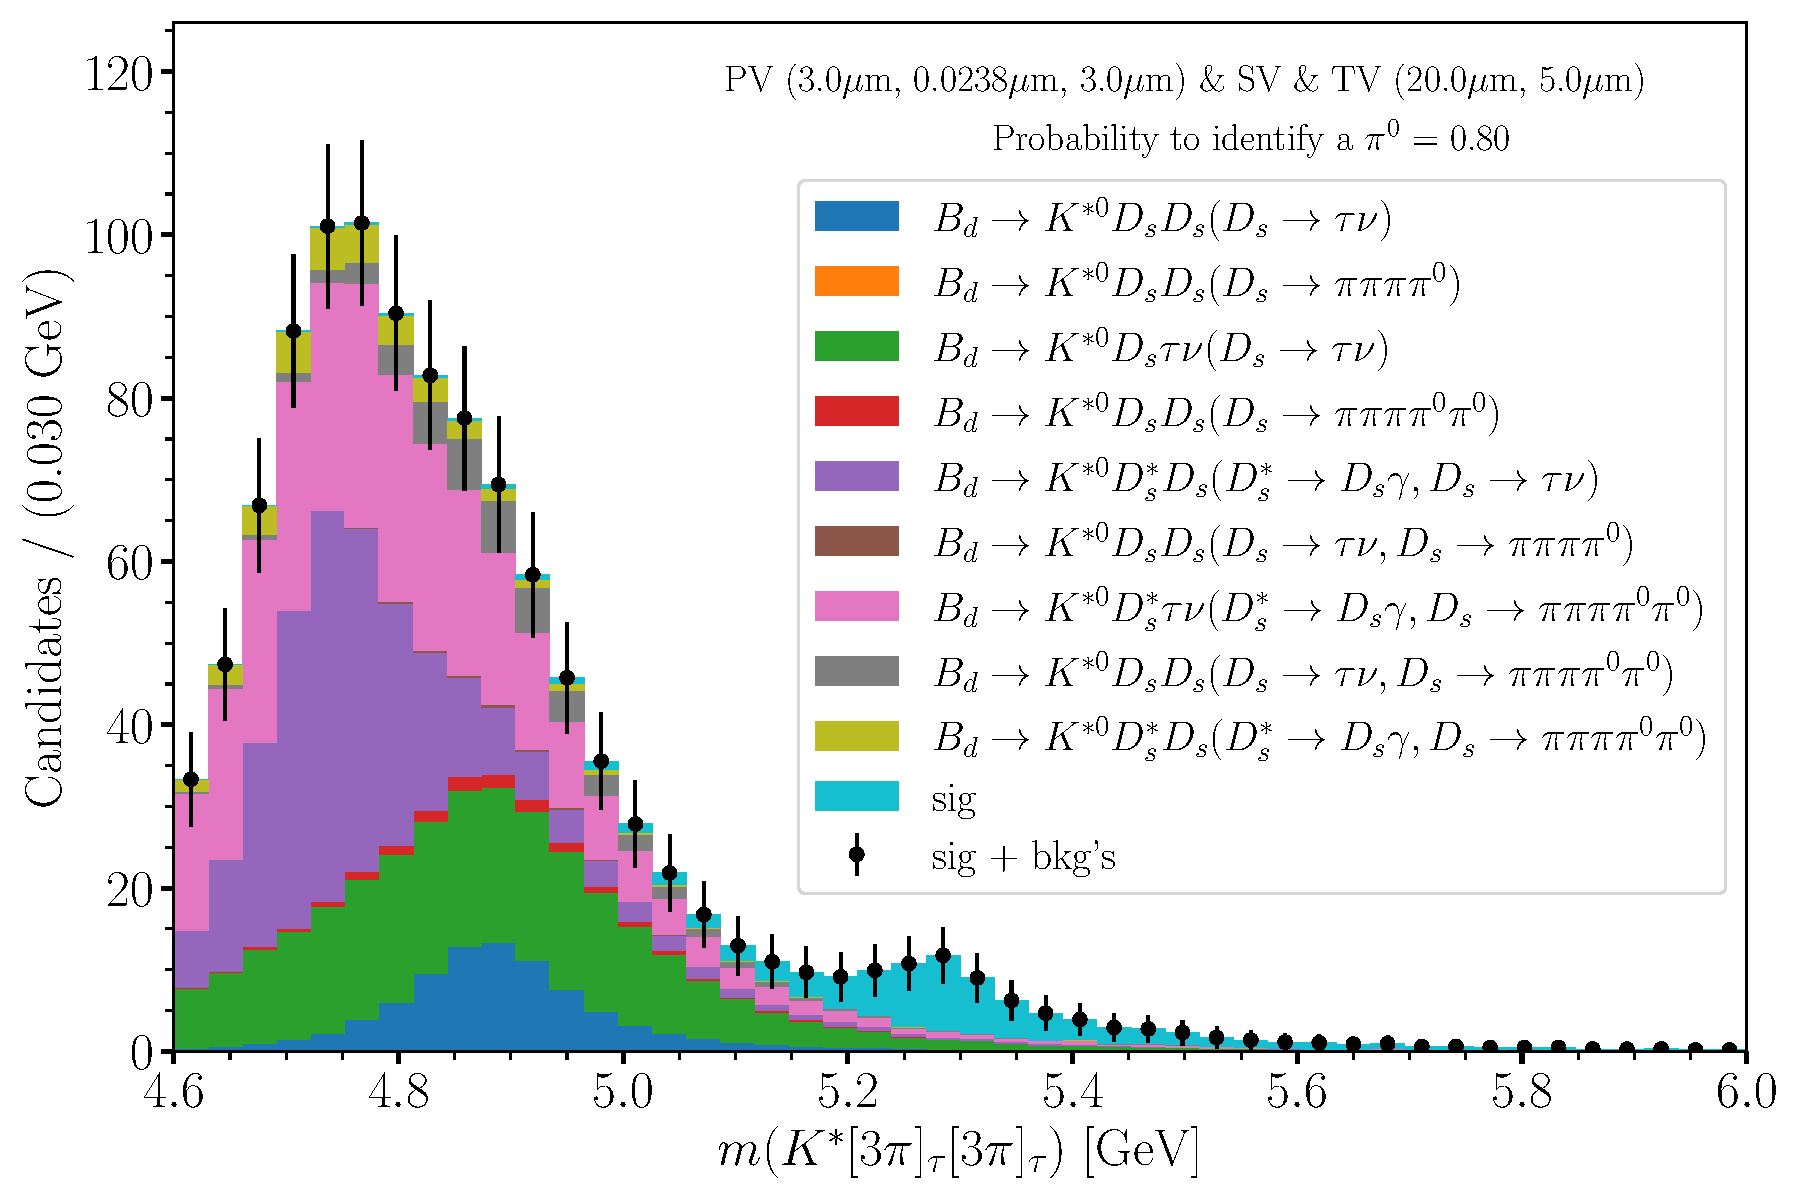
\includegraphics[width=0.67\textwidth]{Physics/DetectorRequirements/Figs/KstarTauTau_mass_20_5.pdf}
\caption{Distribution of the mass of the \PB candidates after the full selection, 
assuming that the secondary and tertiary vertices can be reconstructed with 
a resolution of 5\,$\mu$m (20\,$\mu$m) in the transverse (longitudinal) direction. 
The normalisation corresponds to a total of $6 \times 10^{12}$ produced \PZ bosons.}
\label{fig:KstarTauTau_mass}
\end{figure}

When both \PGt leptons decay into three charged pions and a neutrino, 
there are enough kinematic constraints to completely reconstruct the decay, as illustrated in Fig.~\ref{fig:KstarTauTau_decaychain}. 
The \PGt decay vertices (TV) are obtained from their daughter pion tracks. 
The secondary vertex (SV) is reconstructed from the two tracks (the kaon and the pion) produced by the $\PK^*$ decay. 
The flight direction of each \PGt is then determined from the line that joins the SV to each corresponding TV. 
The component of the neutrino momentum that is transverse to this flight direction is obtained as the opposite 
of the transverse component of the momentum of the three charged pions. 
The \PGt mass constraint finally provides the remaining longitudinal component of the neutrino momentum.
Clearly, this reconstruction relies critically on the precise reconstruction of the secondary and tertiary vertices. 

Several $\PQb \to \PQc \PAQc \PQs$ and $\PQb \to \PQc \PGt \PGn$ transitions lead to final states that are similar to that of the signal, 
apart from the presence of additional neutrinos and neutral pions; 
a powerful \PGpz identification is needed to suppress these backgrounds. 
A \PGpz identification efficiency of 80\% is assumed here. 
A multi-variate analysis allows the background to be reduced to a manageable, albeit still large, level. 
As an example, Fig.~\ref{fig:KstarTauTau_mass} shows the distribution of the mass of the \PB candidates 
for a case where the resolution of the position of the secondary and tertiary vertices is 
20\,$\mu$m in the longitudinal direction and 5\,$\mu$m in the transverse 
direction\footnote{For each tertiary or secondary vertex, the longitudinal direction is defined by the flight direction of the decaying particle.}. 
The remaining background under the \PB mass peak is dominated by irreducible background processes.

The numbers of signal ($N$) and background events are determined in the 5.0--6.0\,GeV range of invariant mass from a maximum likelihood fit. 
The significance of the signal in this range is used as a conservative figure of merit of the reconstruction performance. 
This significance has been determined for several assumptions on the vertex resolution. 
It shows a very strong dependence on the resolution of the position of the secondary and tertiary vertices in the transverse 
direction\footnote{The dependence on the resolution in the longitudinal direction is much milder.}, 
as can be seen from the black dots in Fig.~\ref{fig:KstarTauTau_vertexResolutions}. 
With an event sample corresponding to $6 \times 10^{12}$ produced \PZ bosons, 
a resolution better than $\sim$\,4.3\,$\mu$m is needed to see evidence (3\,$\sigma$) of the decay mode under study 
and it should be better than $\sim$\,2.2\,$\mu$m for the observation (5\,$\sigma$) of this decay. 
With the version of the IDEA detector that is used as a baseline for this report this resolution is only 5\,$\mu$m, 
as shown by the blue star symbol in Fig.~\ref{fig:KstarTauTau_vertexResolutions}. 
To reach the evidence and observation thresholds, 
the resolution on the track impact parameters needs to be improved by about 10\% and 40\%, respectively, 
with respect to the nominal IDEA 
resolutions\footnote{Restricting the invariant mass to the 5.2--5.6\,GeV range would yield a local significance of the signal of about 5\,$\sigma$, but this value is obtained assuming an accurate knowledge of the functional shapes of signal and background candidates, which requires a study that goes beyond the scope of this work.}.

\begin{figure}[t]
\centering
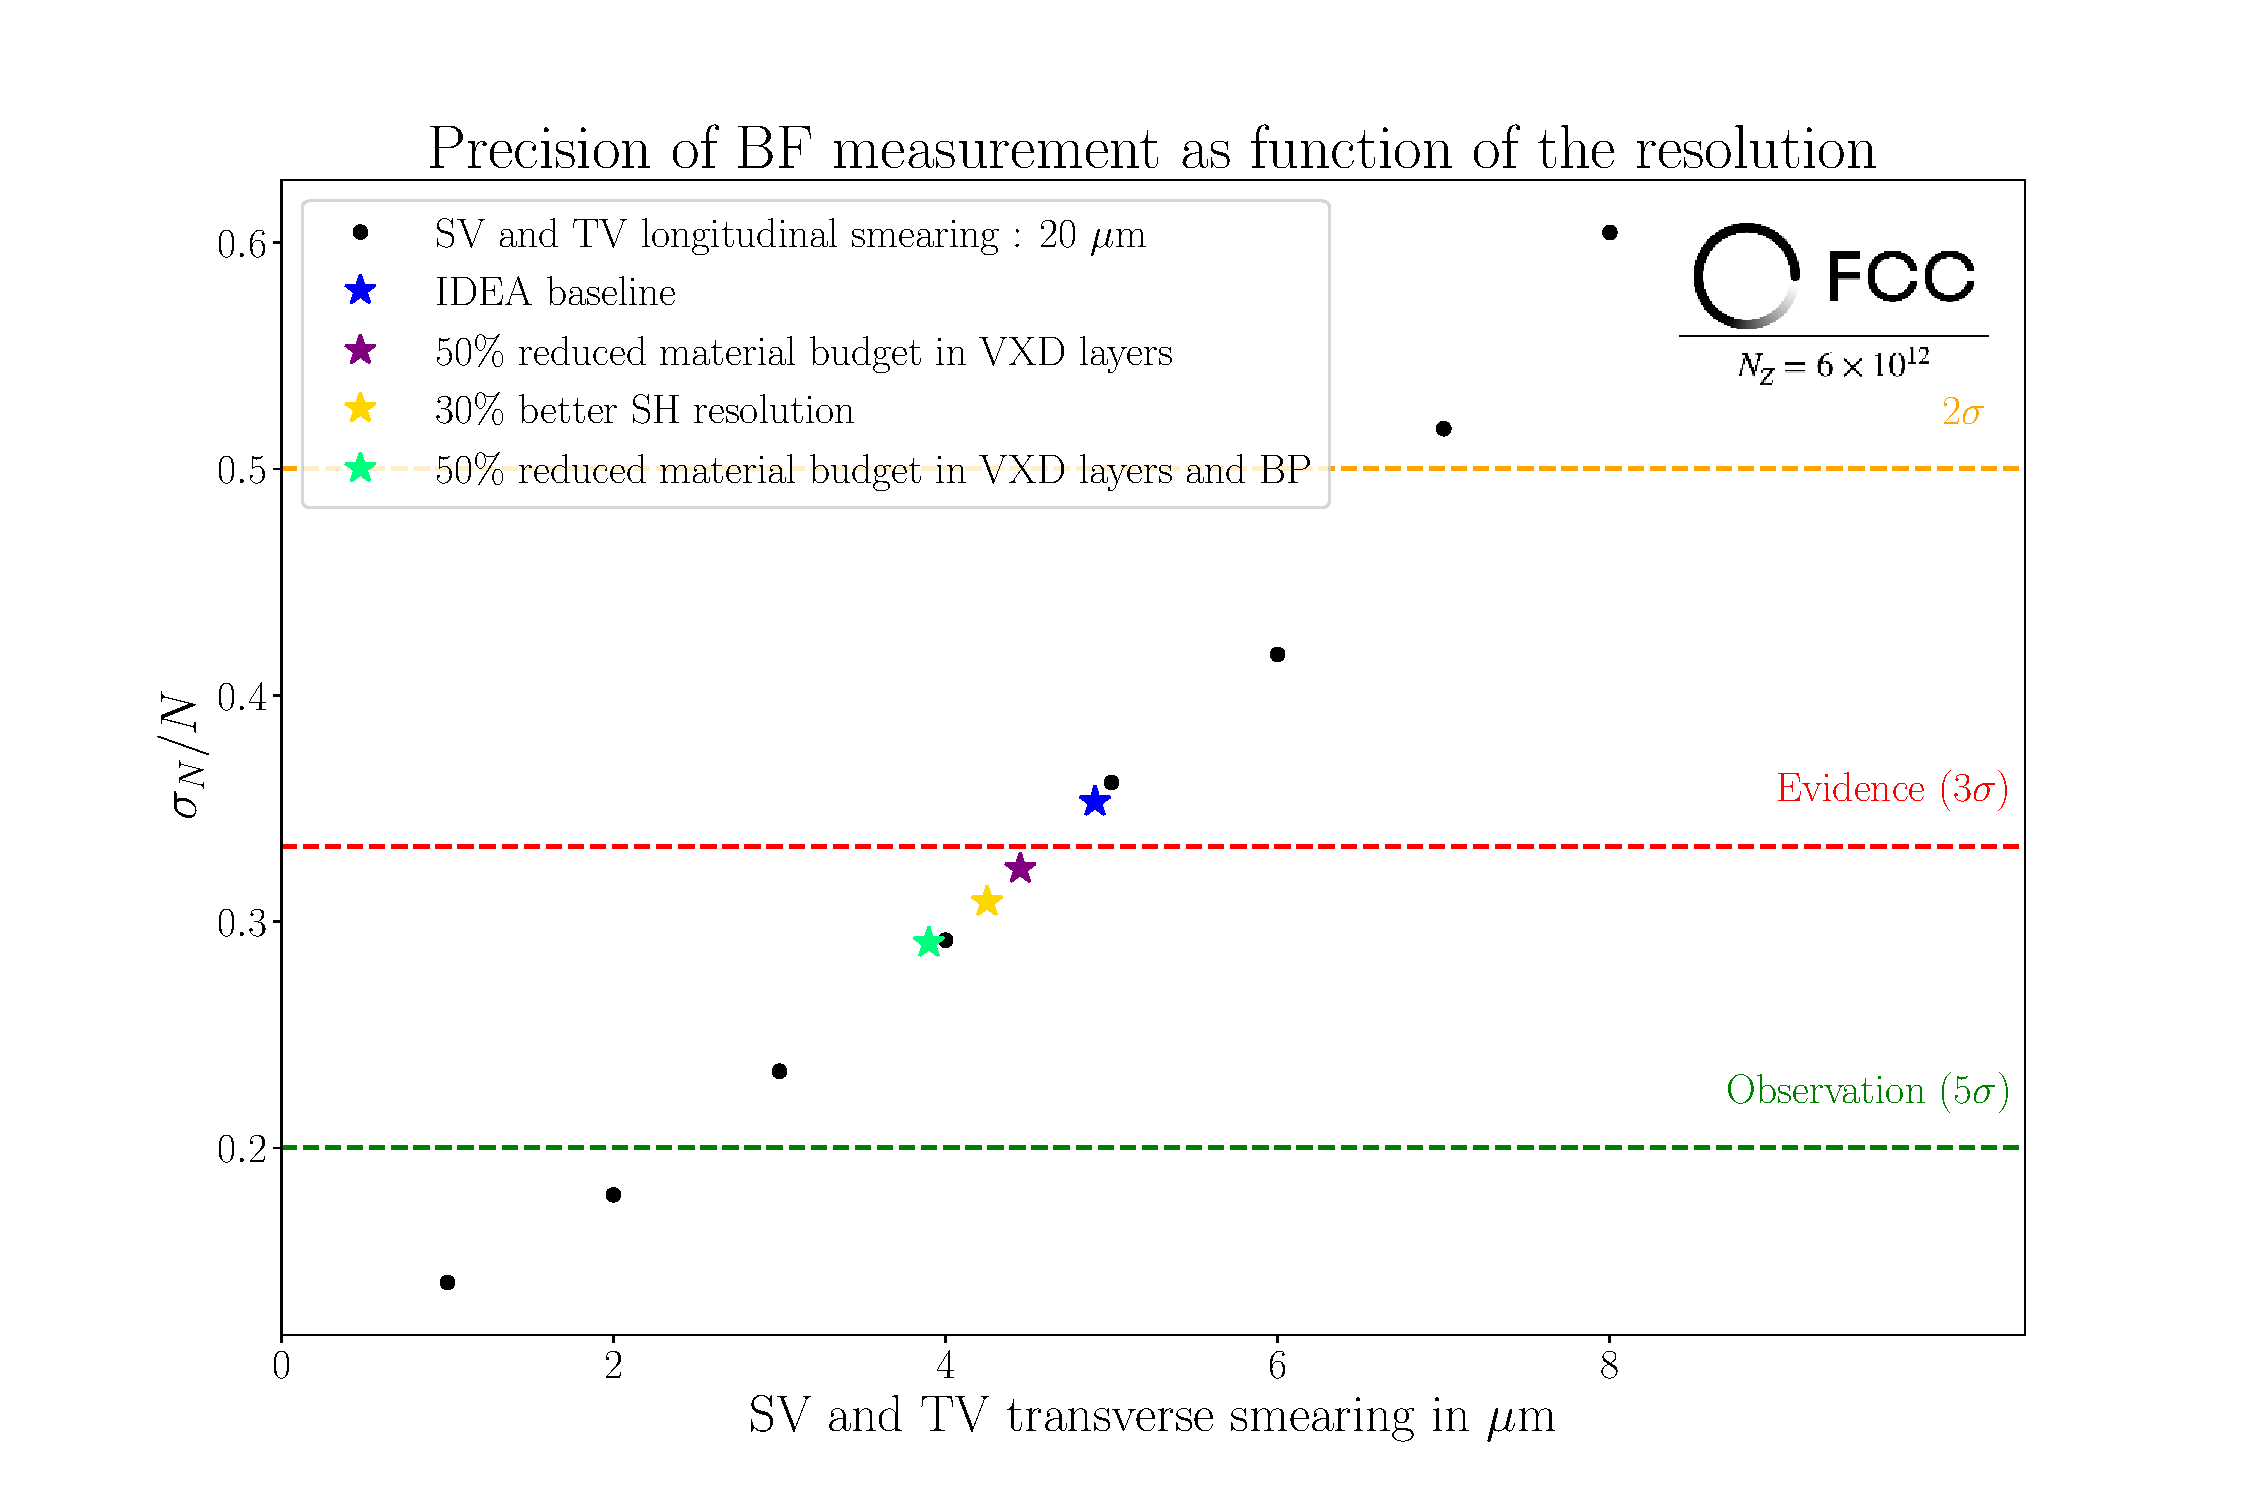
\includegraphics[width=0.7\textwidth]
{DetectorRequirements/Figs/KstarTauTau_vertexResolutions_final.pdf}
\caption{Statistical uncertainty on the $\PB \to \PK^* \PGt \PGt$ branching fraction expected 
from an event sample corresponding to $6 \times 10^{12}$ \PZ bosons, 
as a function of the resolution of the position of the secondary and tertiary vertices, in the transverse direction. 
The blue star shows the precision expected with the version of the IDEA detector used in the nominal simulations. 
The additional star symbols show how the sensitivity improves in alternative simulations of the IDEA detector.}
\label{fig:KstarTauTau_vertexResolutions} 
\end{figure}

In order to investigate if and how these improvements can be achieved, additional \textsc{Delphes} signal samples have been produced, 
with an alternative tracker description, with less tracker 
material\footnote{The decay of interest comprises eight charged particles plus two neutrinos and, hence, features low momentum charged particles to be reconstructed. 
The reduction of the material is therefore one natural improvement to test, in view of minimising multiple Coulomb scattering in the resolution sources.} 
and an improved single hit resolution. 
The results are shown in Fig.~\ref{fig:KstarTauTau_vertexResolutions} by the additional star symbols.
An improvement of the single hit resolution in the VXD layers by 30\% 
(i.e., from 3 to 2\,$\mu$m in the barrel layers) 
brings the sensitivity beyond the 3\,$\sigma$ evidence threshold, as shown by the yellow symbol. 
This threshold is also reached with a 50\% reduction of the VXD material, as shown by the magenta symbol. 
However, the impact of this sole improvement is limited by the material of the beam pipe, 
which causes charged particles to experience multiple scattering before they enter the detector. 
Indeed, in the nominal IDEA simulations used here, the material of the beam pipe is twice that of a VXD layer, 
so that to profit from the reduction in the material of the VXD layers the beam pipe transparency also needs to be increased. 
The green symbol in Fig.~\ref{fig:KstarTauTau_vertexResolutions} shows that, 
by reducing by 50\% the material of both the beam pipe and the VXD layers, 
the sensitivity increases to about 3.5\,$\sigma$, under the SM hypothesis for the considered branching fraction. 
Additional handles will be exploited to increase the sensitivity beyond the 5\,$\sigma$ discovery level.

\subsubsection{Vertex resolutions and heavy-flavour electroweak precision observables}
\label{sec:PhysPerf_HF_EWPO}

The FCC-ee operation at the \PZ-pole offers an immense potential for the measurement of the heavy-quark electroweak precision observables, 
the partial decay-width ratios $R_{\PQb (\PQc)} = \Gamma(\PZ \to \PQb \PAQb \, (\PQc \PAQc) ) \,/\, \Gamma(\PZ \to \text{hadrons})$, 
and the heavy-quark forward-backward production asymmetries $A_{\text{FB}}^{\PQb (\PQc)}$. 
A huge improvement of the statistical uncertainty is expected, with respect to the LEP measurements (by up to a factor of 2000), 
thanks not only to the large luminosity increase but also to the improvements in vertex detector technologies and tagging algorithms.
Experimental strategies that go beyond the current state-of-the-art methods also have to be developed, 
in order to reduce the systematic uncertainties in these measurements, down to a level commensurate with the expected statistical precision.
Earlier measurements have shown that the contamination from light quarks is a large source of systematic uncertainty. 
Taking advantage of the very large number of \PZ bosons that will be produced at FCC-ee, 
a novel tagging technique has been pioneered in Ref.~\cite{note_Lars} for measuring $R_{\PQb}$
and $A_{\text{FB}}^{\PQb}$, which relies on the exclusive reconstruction of a selected list of \PQb-hadron decay modes. 
It allows hemispheres containing a \PQb-hadron to be tagged with a purity larger than 99.8\% and, 
using selected decay modes of charged \PB mesons, the charge of the hemisphere is determined unambiguously. 
After removing the contamination from light quark processes, 
the remaining source of systematic uncertainty for the $R_{\PQb}$ measurement is the correlation of tagging efficiencies 
between the two hemispheres of an event. 
This uncertainty has been studied in detail in Ref.~\cite{note_Lars}, 
using generated events passed through a full simulation (including the reconstruction steps) of the CLD detector. 
In particular, an improved selection of the \PQb-hadron tracks based on their displacement with respect to the luminous region 
has been shown to minimise the impact on the  uncertainty of the exact knowledge of the correlation. 
The hemisphere correlation would need to be known with a relative precision of only 10\% 
to ensure that the corresponding systematic uncertainty on $R_{\PQb}$ is similar to the statistical uncertainty, at the level of 0.015\%. 
This results in a $R_{\PQb}$ determination that is 20 times more precise than the current value, with a lot of potential to do even better.
For the measurement of $A_{\text{FB}}^{\PQb}$, the remaining source of systematic uncertainty is the size of the QCD corrections. 
By exploiting acolinearity~\cite{AlcarazMaestre:2020fmp} or \PQb-hadron energy selection requirements, 
these corrections would need to be known with a relative uncertainty of 1\% for the statistical and systematic uncertainties 
to contribute equally to the total uncertainty. 
As a result, an improvement by a factor of 50 compared to the precision of the average of the LEP measurements would be obtained.

These very small uncertainties motivate the use of exclusively reconstructed hadrons to measure $R_{\PQc}$ as well. 
A first study, described in Ref.~\cite{note_Lars_Rc}, exploits $\PADz \to \PKp \PGpm$ decays. 
The main contamination arises from $\PZ \to \PQb \PAQb$ events and needs to be reduced as much as possible 
to reach the expected statistical precision of $5.3 \times 10^{-5}$ 
(corresponding to an improvement by a factor of about 60 compared to the statistically most precise measurement 
from the SLD Collaboration~\cite{SLD:2005zyw}). 
This contamination can be reduced by demanding that the `pointing angle', 
i.e., the angle between the \PADz momentum and the line that joins the primary vertex and the decay vertex of the \PADz, be close to zero. 
Figure~\ref{fig:Rc_Omega} illustrates how a cut on the cosine of this angle, $\Omega$, separates the signal from the background. 
The measurement of $\Omega$ clearly depends on the reconstruction of the vertices, 
and the figure also shows how the discrimination power increases when the resolution on the longitudinal and transverse track impact parameters improves. 

\begin{figure}[t]
\centering
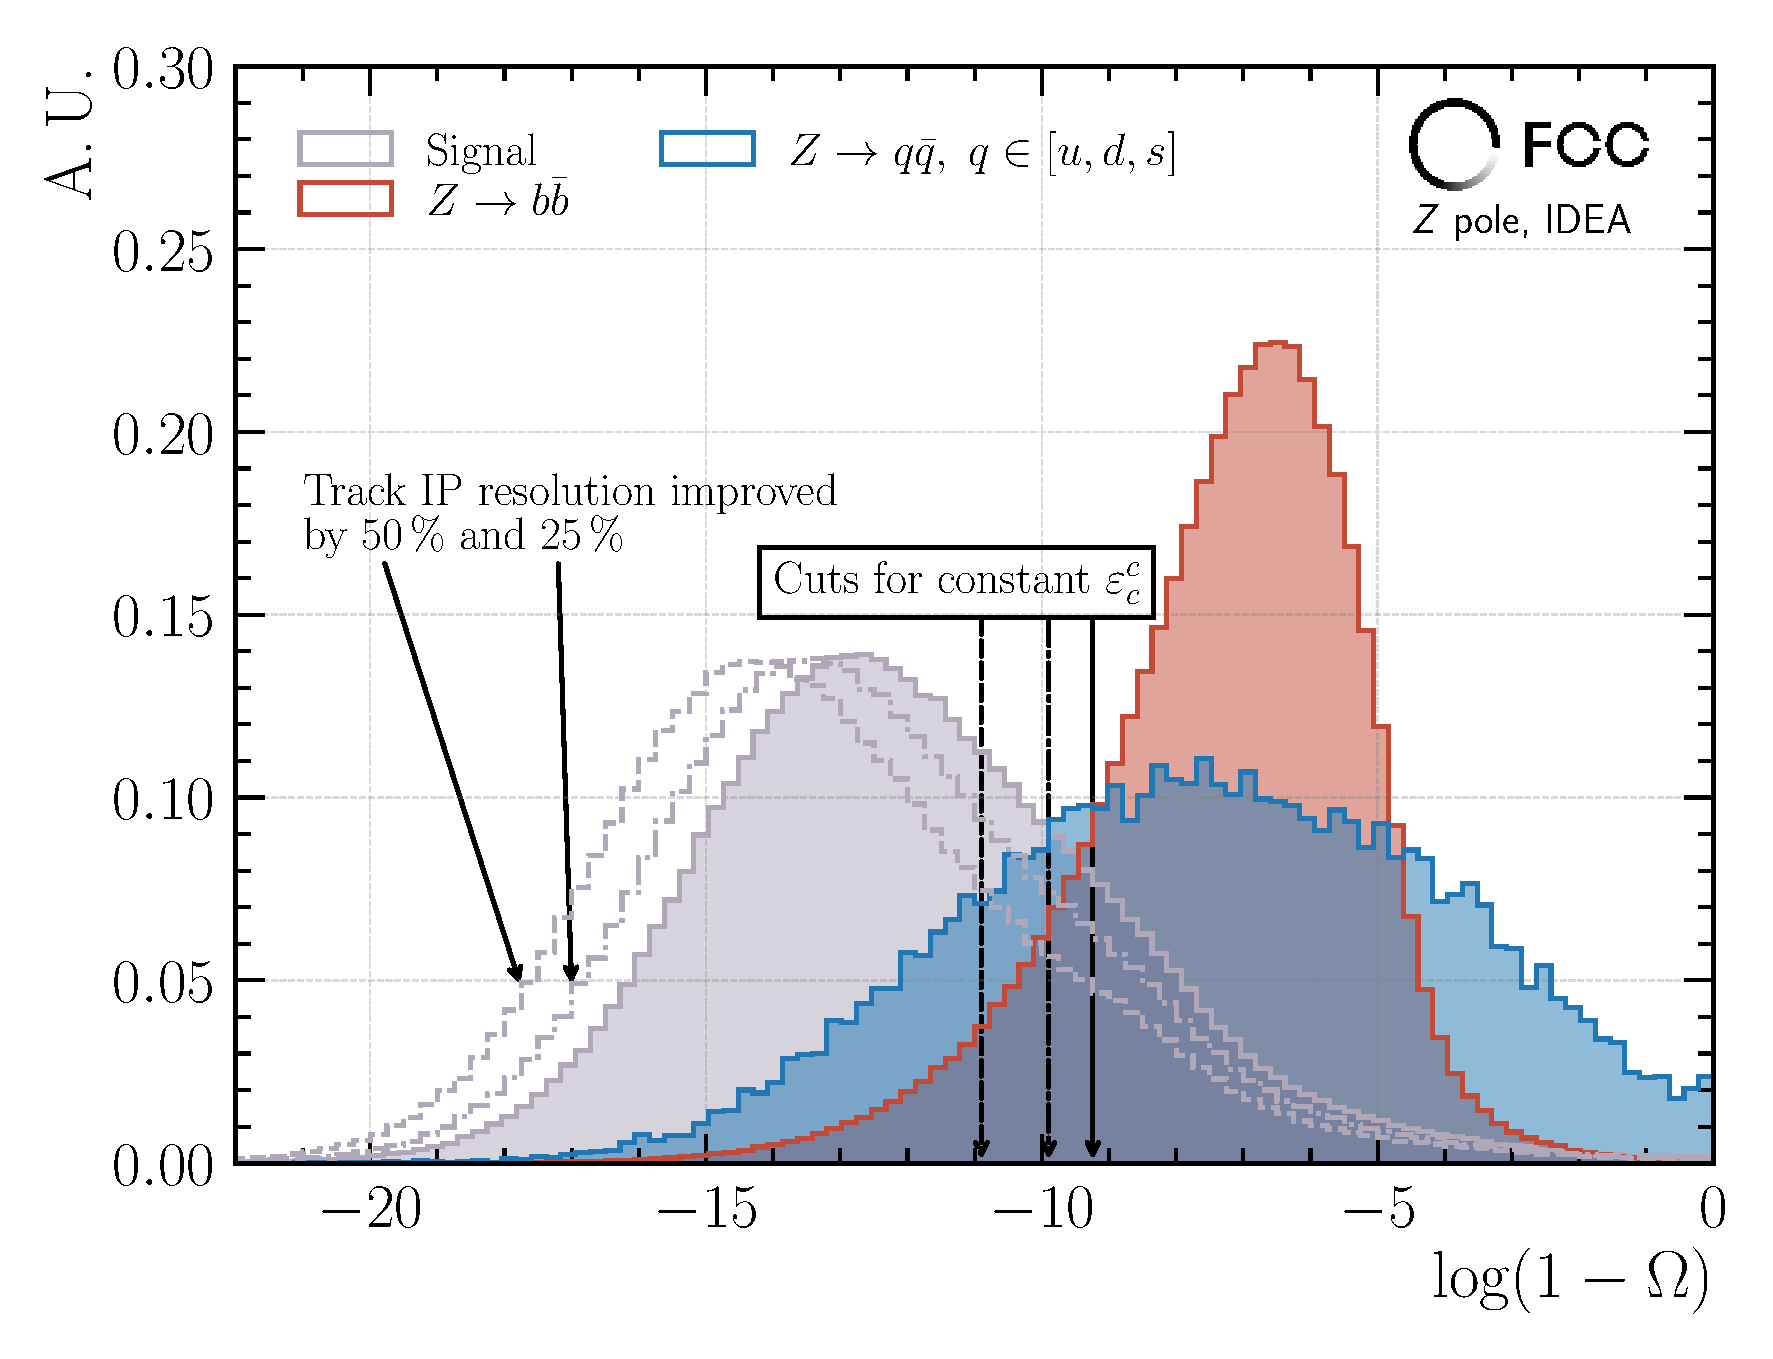
\includegraphics[width=0.7\textwidth]{DetectorRequirements/Figs/Rc_Omega.pdf}
\caption{Distribution of the pointing variable $\log (1 - \Omega)$ for signal and background events, 
where $\PADz \to \PKp \PGpm$ decays (and their charge-conjugates) are used to tag charmed hemispheres. 
The dashed and dash-dotted histograms show how the discrimination improves 
when the resolution of track impact parameters is improved by 25\% and 50\%, respectively, with respect to the nominal IDEA performance.}
\label{fig:Rc_Omega}
\end{figure}

\subsubsection{Alignment, overall scale of the detector, and the measurement of the tau lifetime}
\label{sec:PhysPerf_Taulifetime}

Precise measurements of the mass, the lifetime, and the leptonic branching fraction of the tau offer a crucial test of lepton flavour universality (LFU) since, 
up to small radiative and electroweak corrections, 
the following relation~\cite{Pich:2013lsa,CLEO:1996oro} holds between the muon and tau masses, 
their lifetimes $\tau_{\PGm}$ and $\tau_{\PGt}$, 
their charged-current coupling constants $g_{\PGm}$ and $g_{\PGt}$, 
and their branching fractions into electrons and neutrinos:
\begin{equation}
\left(\frac{g_{\PGt}}{g_{\PGm}}\right)^2 \simeq 
\frac{\tau_{\PGm}}{\tau_{\PGt}} \, \frac{{\cal{B}}(\PGt \to \Pe\PGnGt\PAGne) }{{\cal{B}}(\PGm \to \Pe\PGnGm\PAGne) }\, \left( \frac{m_{\PGm}}{m_{\PGt}} \right)^5 \, . 
\label{eq:tau_LFU}
\end{equation}
This test, which can be seen as a determination of the Fermi constant from the tau, 
is currently limited by the precision of the \PGt lifetime, $290.3 \pm 0.5$\,fs, 
and by that of the $\cal{B}(\PGt \to \Pe \PGnGt \PAGne)$ branching fraction, $17.82 \pm 0.04 \%$. 
The measurement of $\cal{B}(\PGt \to \PGm \PGnGt \PAGnGm)$ allows additional similar tests of $(g_{\PGt} / g_{\Pe})$ and $(g_{\PGm} / g_{\Pe})$.
With the $\sim$\,$2 \times 10^{11}$ tau pair events expected at Tera-\PZ, and a much improved determination of the three key 
ingredients\footnote{The knowledge of the \PGt lepton mass is also expected to be much improved from pair production threshold measurements at a next-generation tau-factory.} 
of Eq.~(\ref{eq:tau_LFU}), FCC-ee has the potential to test LFU at an unprecedented level. 
In particular, the statistical uncertainty in the tau lifetime is expected to be about 15~ppm~\cite{Lusiani:2024tau}. 
The current measurements, from the Belle and LEP experiments, are statistically limited and, 
for the two single most precise measurements (Belle~\cite{Belle:2013teo} and DELPHI~\cite{DELPHI:2003zcz}), 
the alignment of the vertex detector is the dominant source of systematic uncertainty. 
While this alignment could, at first sight, appear to be a concern in view of a lifetime measurement at the level of 15~ppm  
(which corresponds to a few tens of nm on the flight distance of \PGt leptons produced at 91\,GeV), 
a more careful investigation shows that this is not the case~\cite{Lusiani:2024tau}.
Indeed, the offset on the decay length caused by misalignment effects averages to zero, to first order, 
when integrating over the azimuthal angle, as was first noted in Ref.~\cite{Wasserbaech:1998ur}. 
The expected systematic uncertainty due to misalignment, scaled from the value quoted by DELPHI according to the luminosity increase, is below 4~ppm. 
Other sources of systematic uncertainty have been considered in Ref.~\cite{Lusiani:2024tau}. 
One of them reflects the knowledge of the overall length scale of the vertex detector. 
For this uncertainty to be smaller than one half of the statistical uncertainty on the \PGt lifetime, that scale should be known to better than 5~ppm. 
At LEP and at the \PB-factories this scale was only known to 100~ppm. 
However, recent developments made for the MUonE experiment indicate that a precision of 5~ppm is within reach, thanks to the use of optical techniques~\cite{9803636}. 
The leading systematic uncertainties are expected to be due to the modelling of initial state radiation and to the knowledge of the tau mass, and a total systematic uncertainty of 16~ppm on the tau lifetime is deemed within reach~\cite{Lusiani:2024tau}.

\subsubsection{Preliminary conclusions}

\begin{itemize}

\item One example has been shown where the physics outcome of FCC-ee would gain from having better vertex detector performance than the baseline detectors considered so far. 

\item Minimising the amount of material in front of the vertex detector is important. 
Indeed, the material of the beam pipe is a limiting factor in some cases, 
in particular for observing the rare $\PB \to \PK^{*} \PGt \PGt$ decay.

\item It should be noted that these requirements, tighter than the ones presented for a linear collider detector, 
will have to be reached despite the additional constraints set by the FCC-ee environment on the readout electronics of the detector: 
(i)~its power budget is tighter than for a detector operating at a linear collider 
(since power-pulsing the electronics is not possible with collisions occurring every $\sim$\,20\,ns), 
and (ii)~it should handle a hit rate of about 200\,MHz/cm$^2$ in the innermost vertex detector layer at the \PZ peak (Section~\ref{sec:MDI_backgrounds}).

\end{itemize}

\subsection{Requirements for charged hadron particle identification}
\label{sec:PhysPerf_PID}

Charged hadron particle identification (PID) is essential for the FCC-ee flavour physics programme and brings significant benefits for other areas. 
The momentum range over which good PID capabilities are necessary is broad, in sharp contrast with the PID needs of a \PB-factory. 
For flavour physics, for example, it extends from the lowest momentum of the reconstructed charged-particle tracks up to about 40\,GeV.  
In a gaseous tracker like the IDEA drift chamber, the determination of the number of ionisation clusters per unit length (d$N$/d$x$)
is a promising approach that should allow charged kaons to be efficiently separated from charged pions in a large momentum range, from about 1.5\,GeV to several tens of GeV. 
The expected resolution on d$N$/d$x$ 
is about 2\%\footnote{The promising performance of the d$N$/d$x$ approach as determined from calculations, 
in particular the upper momentum bound, is being checked with test beam data.}, 
significantly better than that of the well-known measurement of ionisation energy per unit length (d$E$/d$x$).

Time-of-flight (TOF) measurements, in a single layer at a distance of about 2\,m from the interaction point, 
fill the gap around 1\,GeV\footnote{This statement holds for a magnetic field of 2\,T; the case of a higher field value is briefly considered in Section~\ref{sec:PhysPerf_TOF}.}, 
where the average energy loss per unit length of kaons and pions is similar. 
However, they can only provide a 3\,$\sigma$ $\PGp / \PK$ separation at low momenta, up to about 3\,GeV with the 30\,ps resolution assumed for the studies reported 
here\footnote{Even with a 10\,ps resolution, the momentum range would only extend up to about 5\,GeV.}. 
Innovative solutions are being studied that would provide good PID capabilities in the absence of a specific energy loss measurement, 
over the large momentum range of interest and despite the tight spatial constraints. 
A conceptual design exists for a compact RICH detector, which looks promising and could comfortably cover the required momentum range~\cite{forty_2024_6g0gs-7kw30, Forty_ARC, Tat_ARC}. 
An overview of the motivations for PID and of the possible detector solutions can be found in Ref.~\cite{Wilkinson:2021ehf}. 
This section illustrates the demands on PID performance with the measurement of the Higgs boson coupling to strange quarks and with two \PB-physics processes.

\subsubsection{Strange tagging and the Higgs boson coupling to strange (and charmed) quarks}
\label{sec:PhysPerf_strangeTagging}

The progress in the development of flavour-tagging algorithms in recent years allows, for the first time, 
a relatively efficient and pure tagging of jets induced by strange quarks. 
Various analysis efforts are ongoing within the circular and linear colliders communities. 
They all rely heavily on the identification power of state-of-the-art machine learning approaches. 

\begin{figure}[ht]
\centering
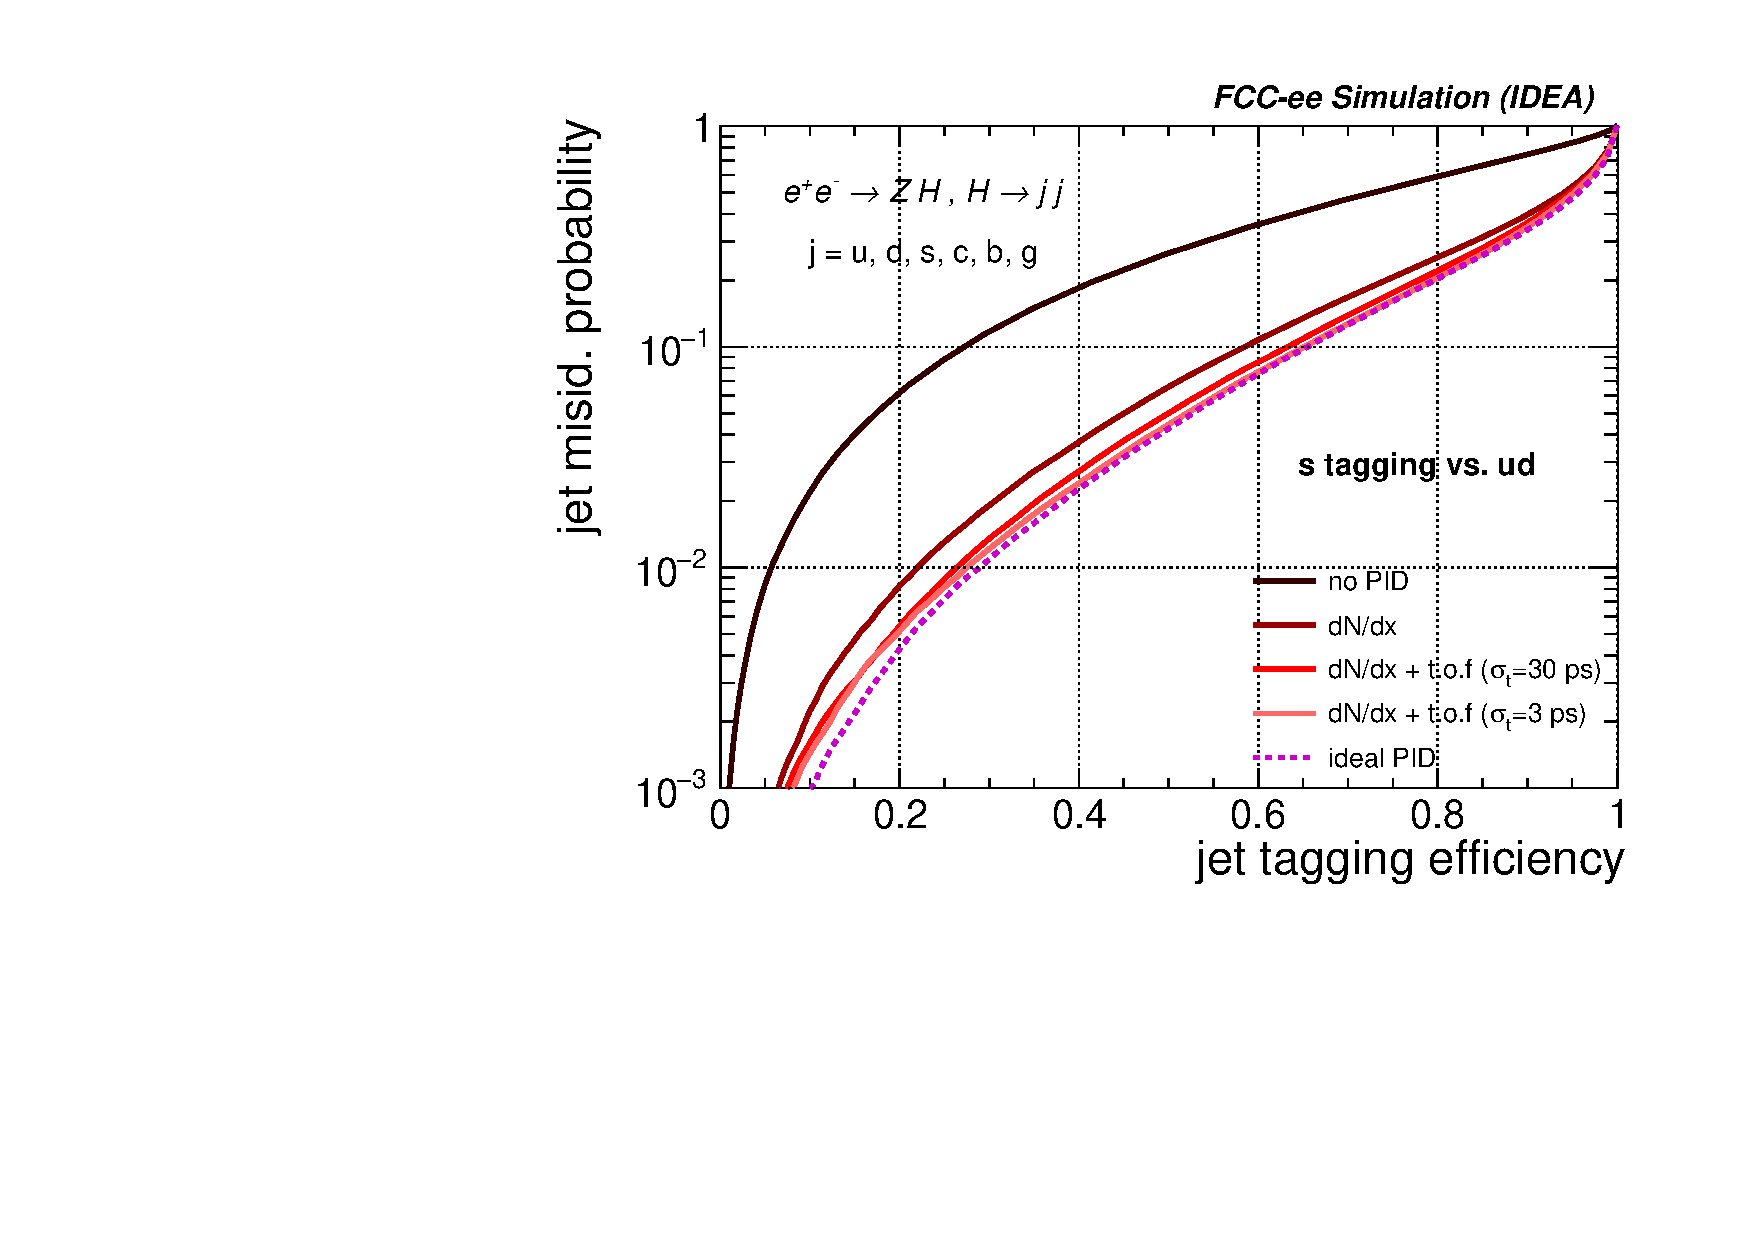
\includegraphics[width=0.49\textwidth]{DetectorRequirements/Figs/StrangeTagging_perf_pid.pdf}
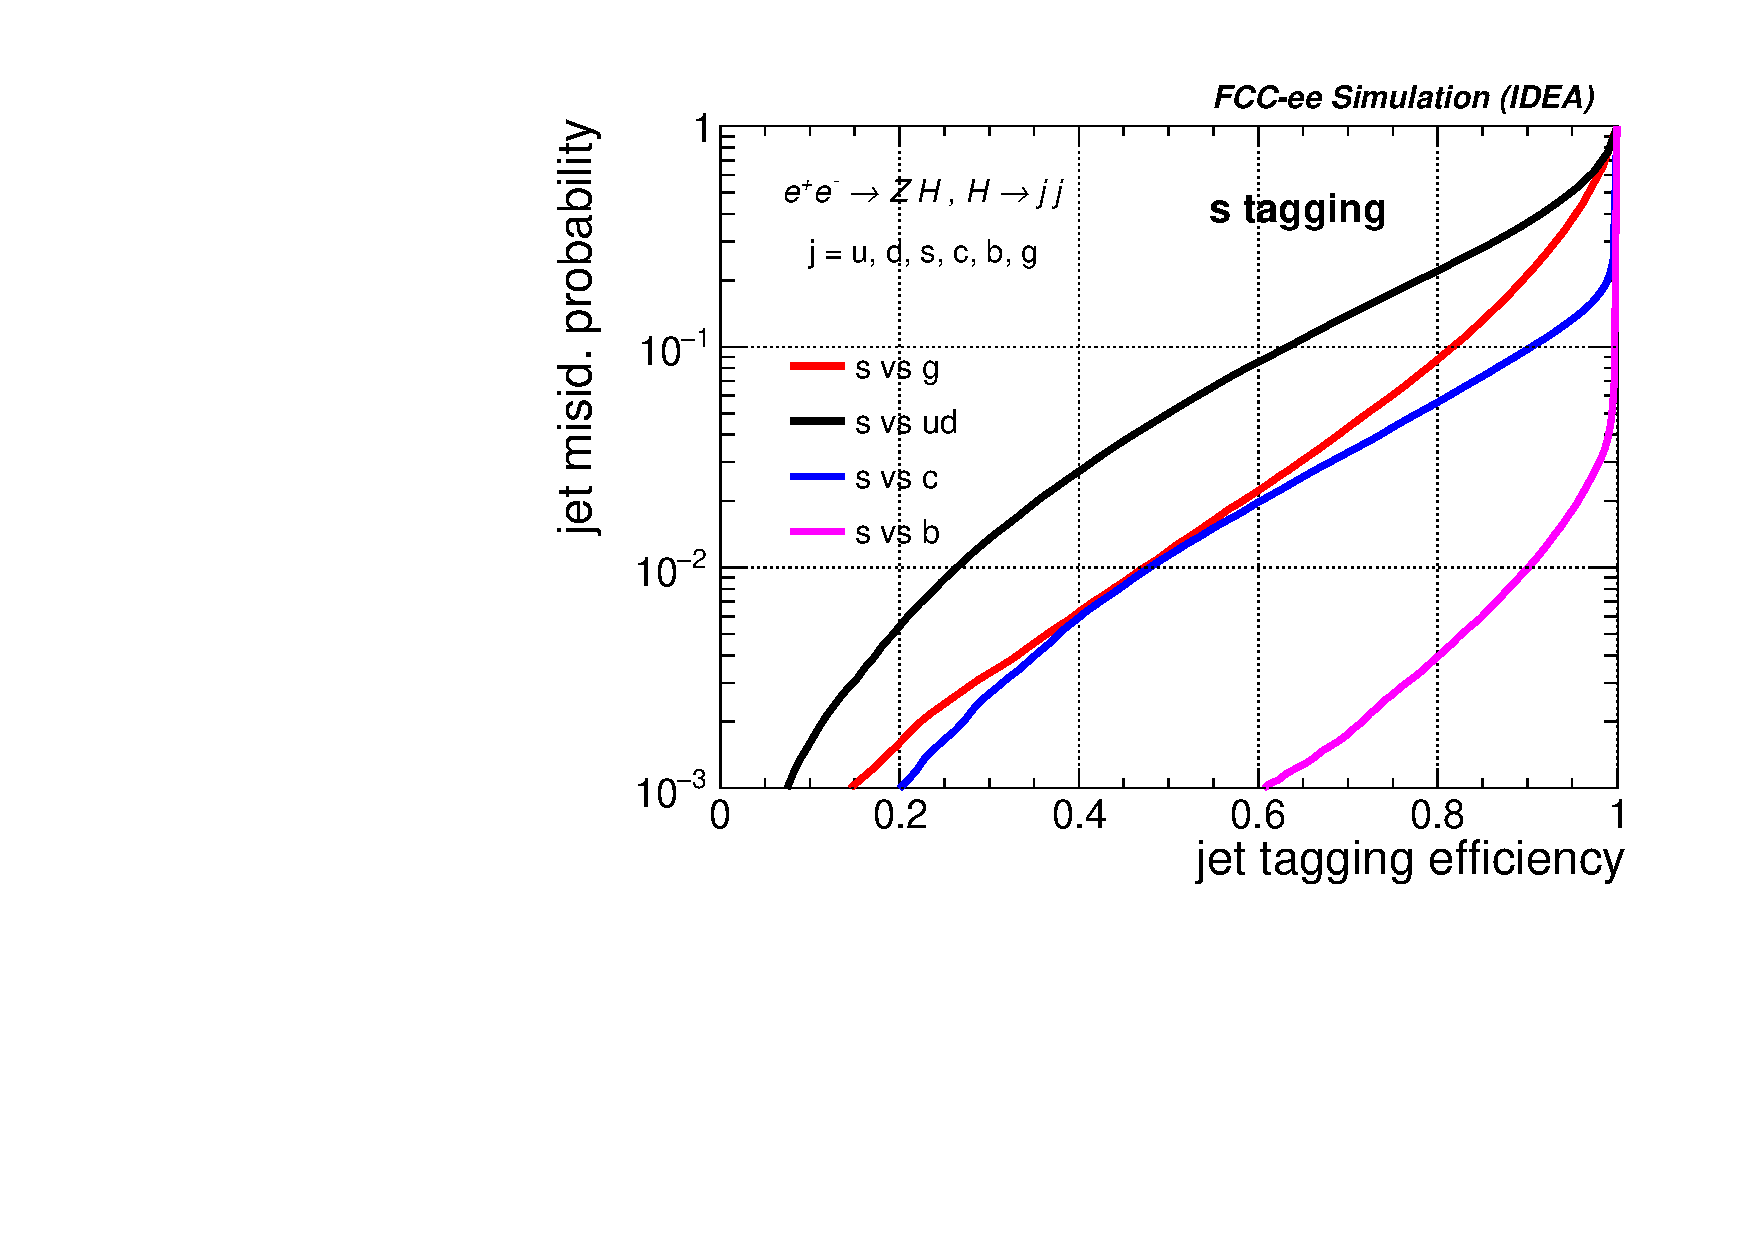
\includegraphics[width=0.49\textwidth]{DetectorRequirements/Figs/StrangeTagging_perf_stag.pdf}
\caption{Performance of strange-quark tagging in jet samples from $\PZ(\PGn \PAGn) \PH$ events at $\sqrt{s} = 240$\,GeV, 
where the Higgs boson decays into quarks of a well-defined flavour or into gluons. 
The left panel shows the impact of PID on the separation power between jets induced by strange quarks and those induced by \PQu or \PQd quarks. 
The right panel shows how the algorithm separates strange jets from all other flavours. 
The `\PQs vs.\ $\PQu\PQd$' (black) curve in the right panel is identical to the red curve in the left panel.}
\label{fig:strange_tagging}
\end{figure}

Figure~\ref{fig:strange_tagging} illustrates the performance of strange-quark tagging with the baseline IDEA detector used for this report, 
using the {\textsc{ParticleNetIDEA}} algorithm~\cite{Bedeschi:2022rnj}. 
As shown in the left panel, when no PID information is provided to the algorithm, 
the separation power between jets induced by strange quarks and those induced by \PQu or \PQd quarks is limited, 
as it mostly comes from the slightly harder energy spectrum of the constituents of a strange 
jet\footnote{The number of reconstructed $\PKS \to \PGpp \PGpm$ decays from displaced tracks associated with the jets (see Section~\ref{sec:PhysPerf_Kshorts}) 
is not yet explicitly included in the set of variables used by the {\textsc{ParticleNetIDEA}} algorithm; adding this variable may improve the performance shown here.}. 
When the specific energy loss measured along the tracks with the cluster counting technique is also used, 
the misidentification probability of jets induced by \PQu or \PQd quarks is reduced by about one order of magnitude, for the same \PQs-quark tagging efficiency. 
In the kinematic range considered here, spanned by quarks produced in $\PZ (\PGn \PAGn) \PH(\PQq \PAQq)$ events at $\sqrt{s} = 240$\,GeV, 
the time-of-flight information only brings a mild performance improvement. 
The right panel of Fig.~\ref{fig:strange_tagging} shows how the algorithm separates strange jets from all other flavours, 
the separation from $\PQu\PQd$ jets being, as expected, the most challenging. 
For a strange-quark tagging efficiency of 80\% (90\%), the mis-tag efficiency of $\PQu\PQd$ jets reaches 20\% (40\%).

This tagging algorithm has been used to categorise $\PZ(\ell \ell, j j) \PH(jj)$ events 
(where $\ell$ stands for \Pe, \PGm or \PGn) 
into mutually orthogonal categories enriched in one of the different Higgs boson decays (Section~\ref{sec:PhysPerf_Hcc}) 
and to extract the Higgs boson branching fractions to $\PQb \PAQb$, $\PQc \PAQc$, $\PQs \PAQs$, and $\Pg\Pg$.
With an integrated luminosity of $10.8$\,ab$^{-1}$, the Higgs boson branching fraction to strange quarks would be measured with a 105\% uncertainty. 
More details can be found in Ref.~\cite{note_Higgs_to_hadrons}.

The anticipated precision on the Higgs boson branching fractions to $\PQc \PAQc$ and $\PQs \PAQs$ has been explored for several particle identification capabilities 
and the result is shown in Fig.~\ref{fig:Hss_versus_PID}. 
Given that charged kaons from strange quark hadronisation feature a hard momentum spectrum, 
it is crucial to have an efficient $\PK/\PGp$ separation at large momenta, as provided by the d$N$/d$x$ cluster counting technique. 
It is remarkable that the expected precision on the measurement of the $\PH \to \PQs \PAQs$ branching fraction, 
obtained by combining d$N$/d$x$ with the time-of-flight technique, 
is almost identical to the asymptotic performance obtained with perfect PID capabilities. 
Conversely, if no PID is assumed, or only assuming ToF, the $\PH \to \PQs \PAQs$ branching fraction measurement cannot be performed, 
given an expected uncertainty in excess of 300\%. 
The PID also plays a non-negligible role in the $\PH \to \PQc\PAQc$ branching fraction measurement, 
by enabling the identification of secondary charged kaons produced in \PD meson decays, 
as shown in the right panel of Fig.~\ref{fig:Hss_versus_PID}. 
A comprehensive discussion on the impact of PID on flavour tagging performance can be found in Ref.\cite{sciandra_2024_gt813-z8602}.

\begin{figure}[ht]
\centering
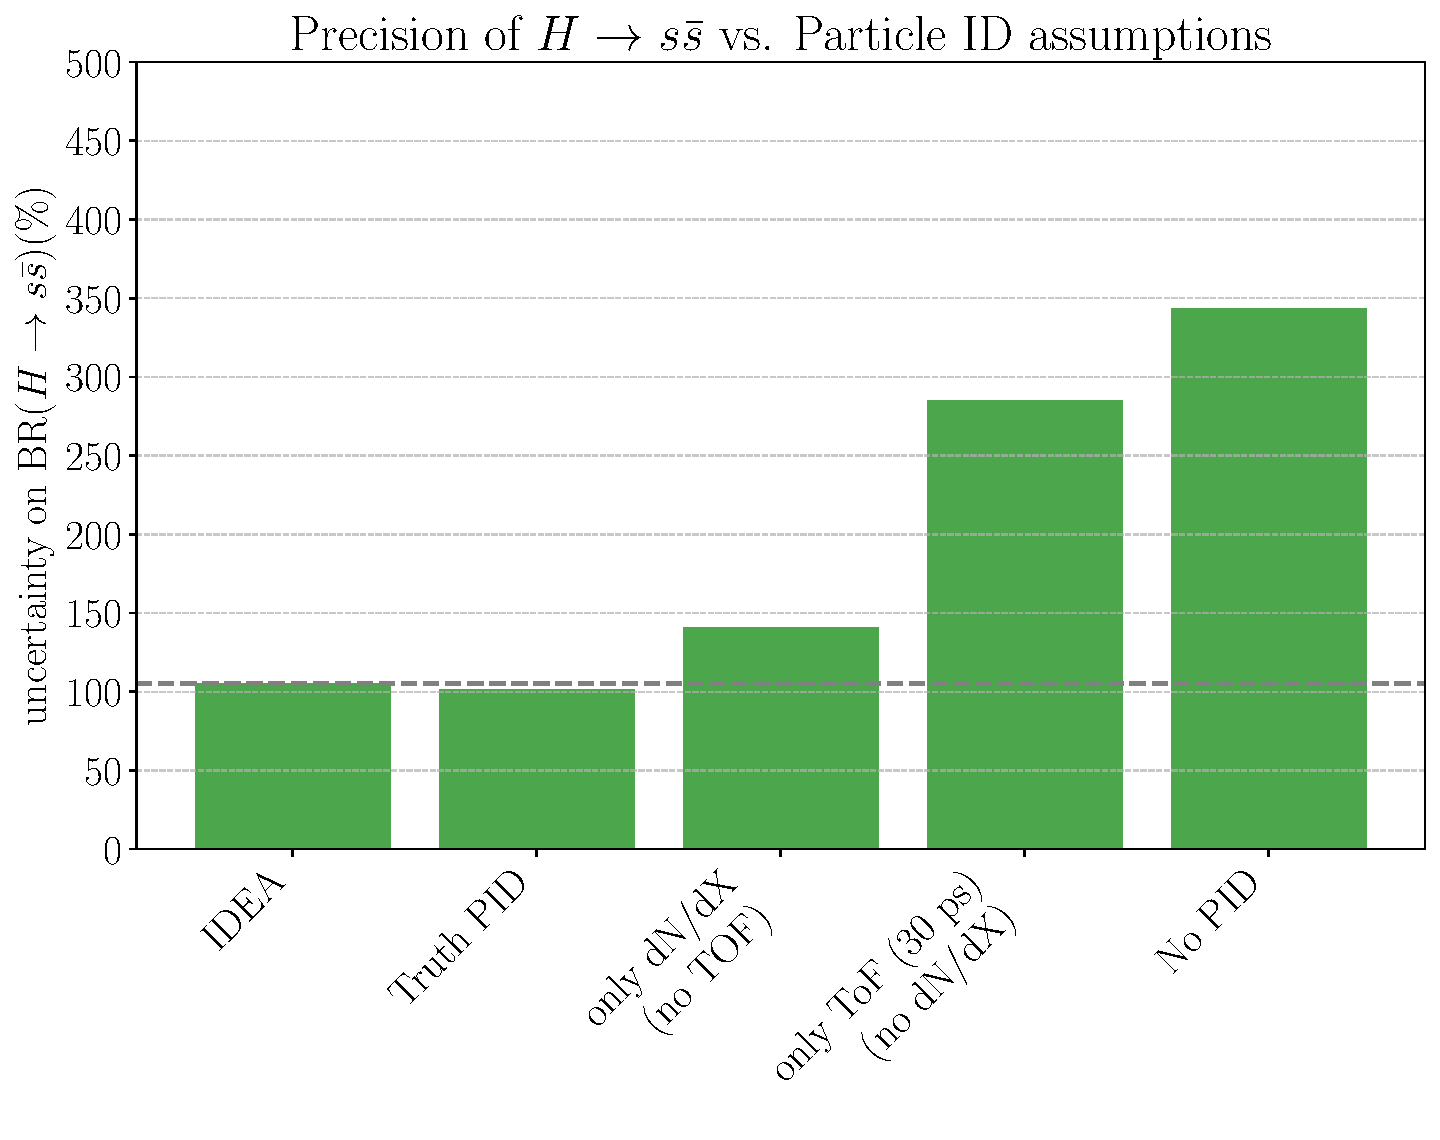
\includegraphics[width=0.49\textwidth]{Physics/DetectorRequirements/Figs/hss_pid.pdf}
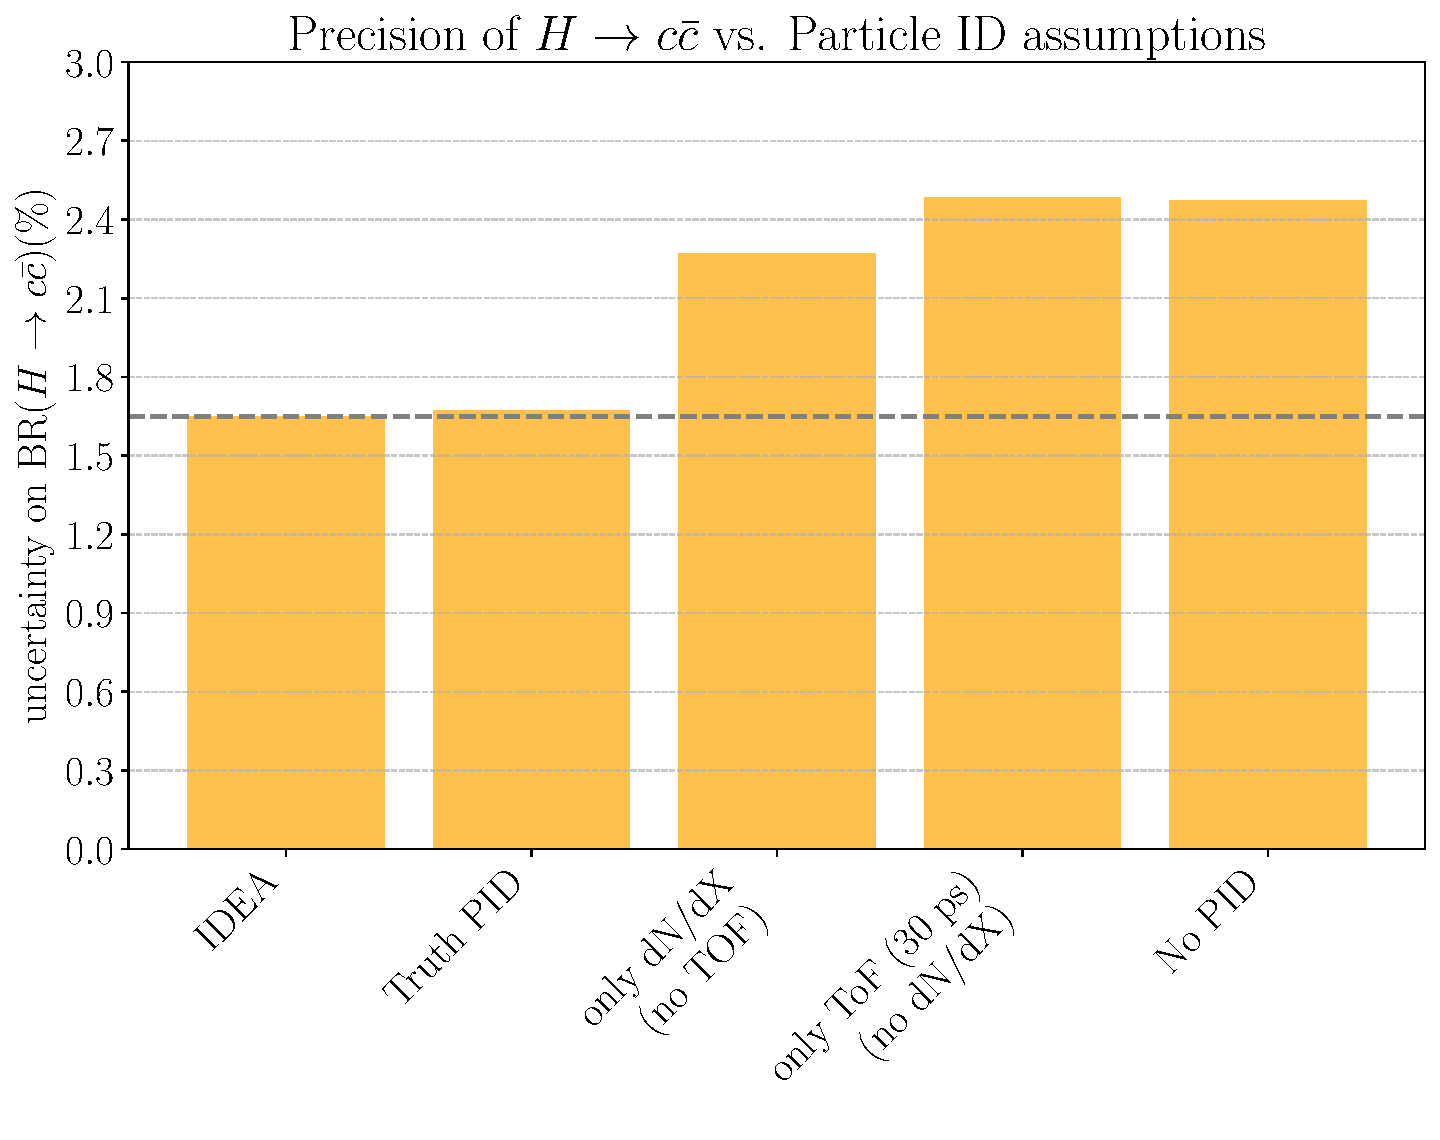
\includegraphics[width=0.49\textwidth]{Physics/DetectorRequirements/Figs/hcc_pid.pdf}
\caption{Relative uncertainty in the $\PH \to \PQs \PAQs$ (left) and $\PH \to \PQc\PAQc$ (right) branching fractions, 
as expected for several assumptions on particle identification performance setups.}
\label{fig:Hss_versus_PID}
\end{figure}

\subsubsection{Separation of \texorpdfstring{\PKpm}{K+-} from \texorpdfstring{\PGppm}{pi+-} and measurement of \texorpdfstring{$\PQb \to \PQs \PGn \PAGn$}{b to s neutrino antineutrino} }

The trillions of $\PQb \PAQb$ events that will be collected, in a clean environment, 
during the Tera-\PZ run at FCC-ee makes it the ideal facility to study rare decays of \PQb~hadrons. 
Among those, the modes corresponding to the $\PQb \to \PQs \PGn \PAGn$ transition are of considerable interest within the flavour physics 
community\footnote{The first evidence for this transition has been recently obtained by the Belle~II Collaboration in the 
$\PBp \to \PKp \PGn \PAGn$ decay channel~\cite{BelleII-EPS2023}. 
In the future, with an integrated luminosity of 50\,ab$^{-1}$, 
Belle~II is expected to measure the corresponding branching fraction with ${\cal{O}}(10\%)$ experimental precision~\cite{Belle-II:2018jsg}.}. 
A first sensitivity study for FCC-ee, using the decays $\PB \to \PK^{*} \PGn \PAGn$ and $\PBs \to \PGf \PGn \PAGn$, is detailed in Ref.~\cite{Amhis:2023mpj}. 
According to the Standard Model, both decays should have branching fractions around $10^{-5}$. 
The current experimental upper limit on the branching fraction of $\PB \to \PK^{*} \PGn \PAGn$ is larger than this prediction by a factor of two, 
while for $\PBs \to \PGf \PGn \PAGn$, the upper limit is two orders of magnitude larger. 
The study looks for a $\PK^{*}$ or a \PGf resonance in a hemisphere with a large amount of missing energy and runs a multi-variate analysis, 
following the strategy described in Ref.~\cite{Zuo:2023dzn}. 
Assuming a perfect PID, the $\PB \to \PK^{*} \PGn \PAGn$ ($\PBs \to \PGf \PGn \PAGn$) signal can be selected with an efficiency of 3.7\% (7.4\%), 
for a signal-to-background ratio of 0.17 (0.13). 
With $6 \times 10^{12}$ \PZ bosons produced, 
this corresponds to a sensitivity of 0.5\% for $\PB \to \PK^{*} \PGn \PAGn$ and of 1.2\% for $\PBs \to \PGf \PGn \PAGn$. 
Here, sensitivity is defined as the relative precision expected on the branching fraction, computed as $\sqrt{S+B} / S$, 
where $S$ and $B$ are the expected numbers of signal and background events, respectively. 
The dependence of this sensitivity on the performance of the $\PGp/\PK$ separation that the detector would achieve is shown in Fig.~\ref{fig:PID_for_bsnunu}. 
With a separation power of 2\,$\sigma$, the loss in sensitivity, compared to what is expected with perfect PID, is marginal, 
but it degrades quickly as the performance worsens. 
The momentum of the kaons involved in these decays peaks at about 3\,GeV, but extends up to 15--20\,GeV, 
hence the PID performance offered by time-of-flight measurements alone is unlikely to be sufficient for this analysis.

\begin{figure}[ht]
\centering
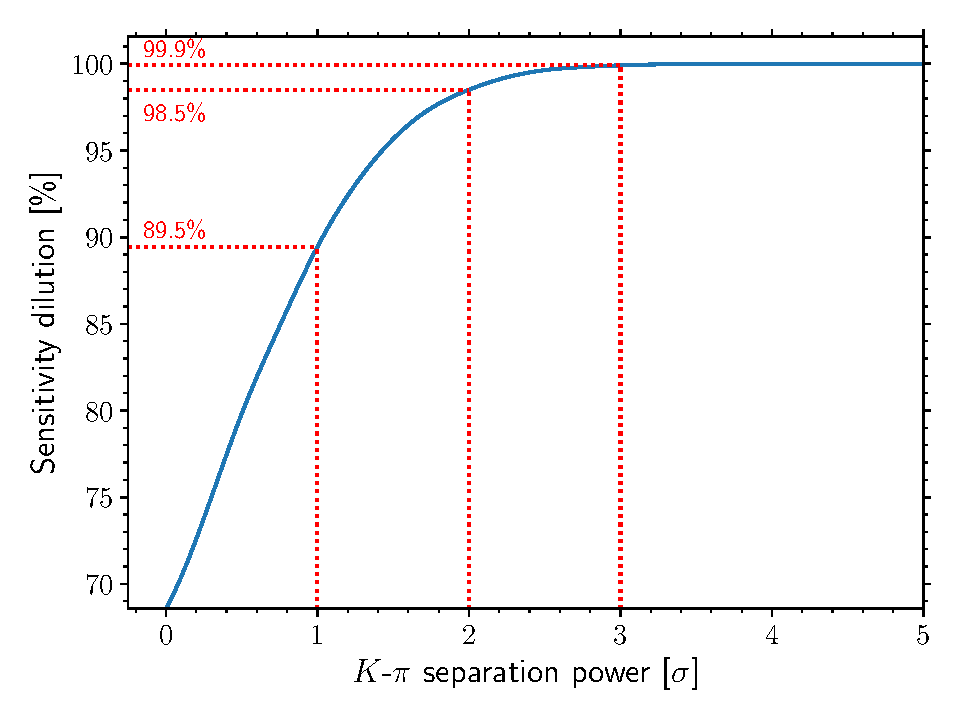
\includegraphics[width=0.495\textwidth]{DetectorRequirements/Figs/Bd2KstNuNu_pid2.pdf} 
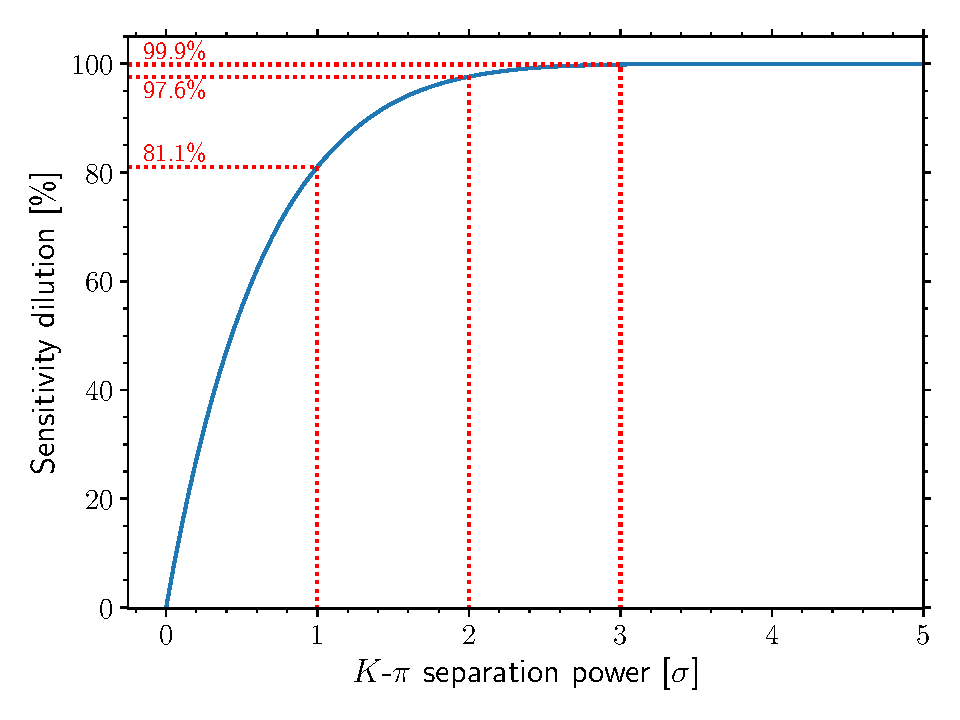
\includegraphics[width=0.495\textwidth]{DetectorRequirements/Figs/Bs2PhiNuNu_pid2.pdf}
\caption{Sensitivity to the $\PB \to \PK^{*} \PGn \PAGn$ (left) and $\PBs \to \PGf \PGn \PAGn$ (right) branching fractions, 
as a function of the $\PGp/K$ separation power, with respect to the sensitivity assuming perfect PID.}
\label{fig:PID_for_bsnunu}
\end{figure}

\subsubsection{Separation of \texorpdfstring{\PKpm}{K+-} from \texorpdfstring{\PGppm}{pi+-} 
and measurement of \texorpdfstring{$\PBs \to \PDs \PK$}{Bs to Ds K} }  
\label{sec:PhysPerf_Bs2DsK}

The measurement of time-dependent CP asymmetries in the decay $\PBs \to \PDs \PK$ is a well-known method to extract the $\gamma$ angle of the CKM matrix, 
which is currently only known with a precision of 4~degrees. 
The prospects for this measurement at FCC-ee have been first studied in Ref.~\cite{Aleksan:2021gii}, using the $\PDs \to \PGf (\PK\PK) \PGp$ decay channel. 
The presence of the \PGf resonance and the absence of neutral particles among the final decay products makes this signal easy to reconstruct. 
A precision on the $\gamma$ angle of a few tenths of a degree was shown to be within reach at FCC-ee, using only this decay 
mode\footnote{A similar sensitivity is expected from the Phase-2 LHCb upgrade, with an integrated luminosity of 300\,fb$^{-1}$~\cite{Charles:2020dfl}. 
The FCC-ee sensitivity can be improved by including other \PDs decay modes, in particular those that include neutral particles (see Section~\ref{sec:PhysPerf:pi0_reco_for_flavour}).}.

\begin{figure}[ht]
\centering
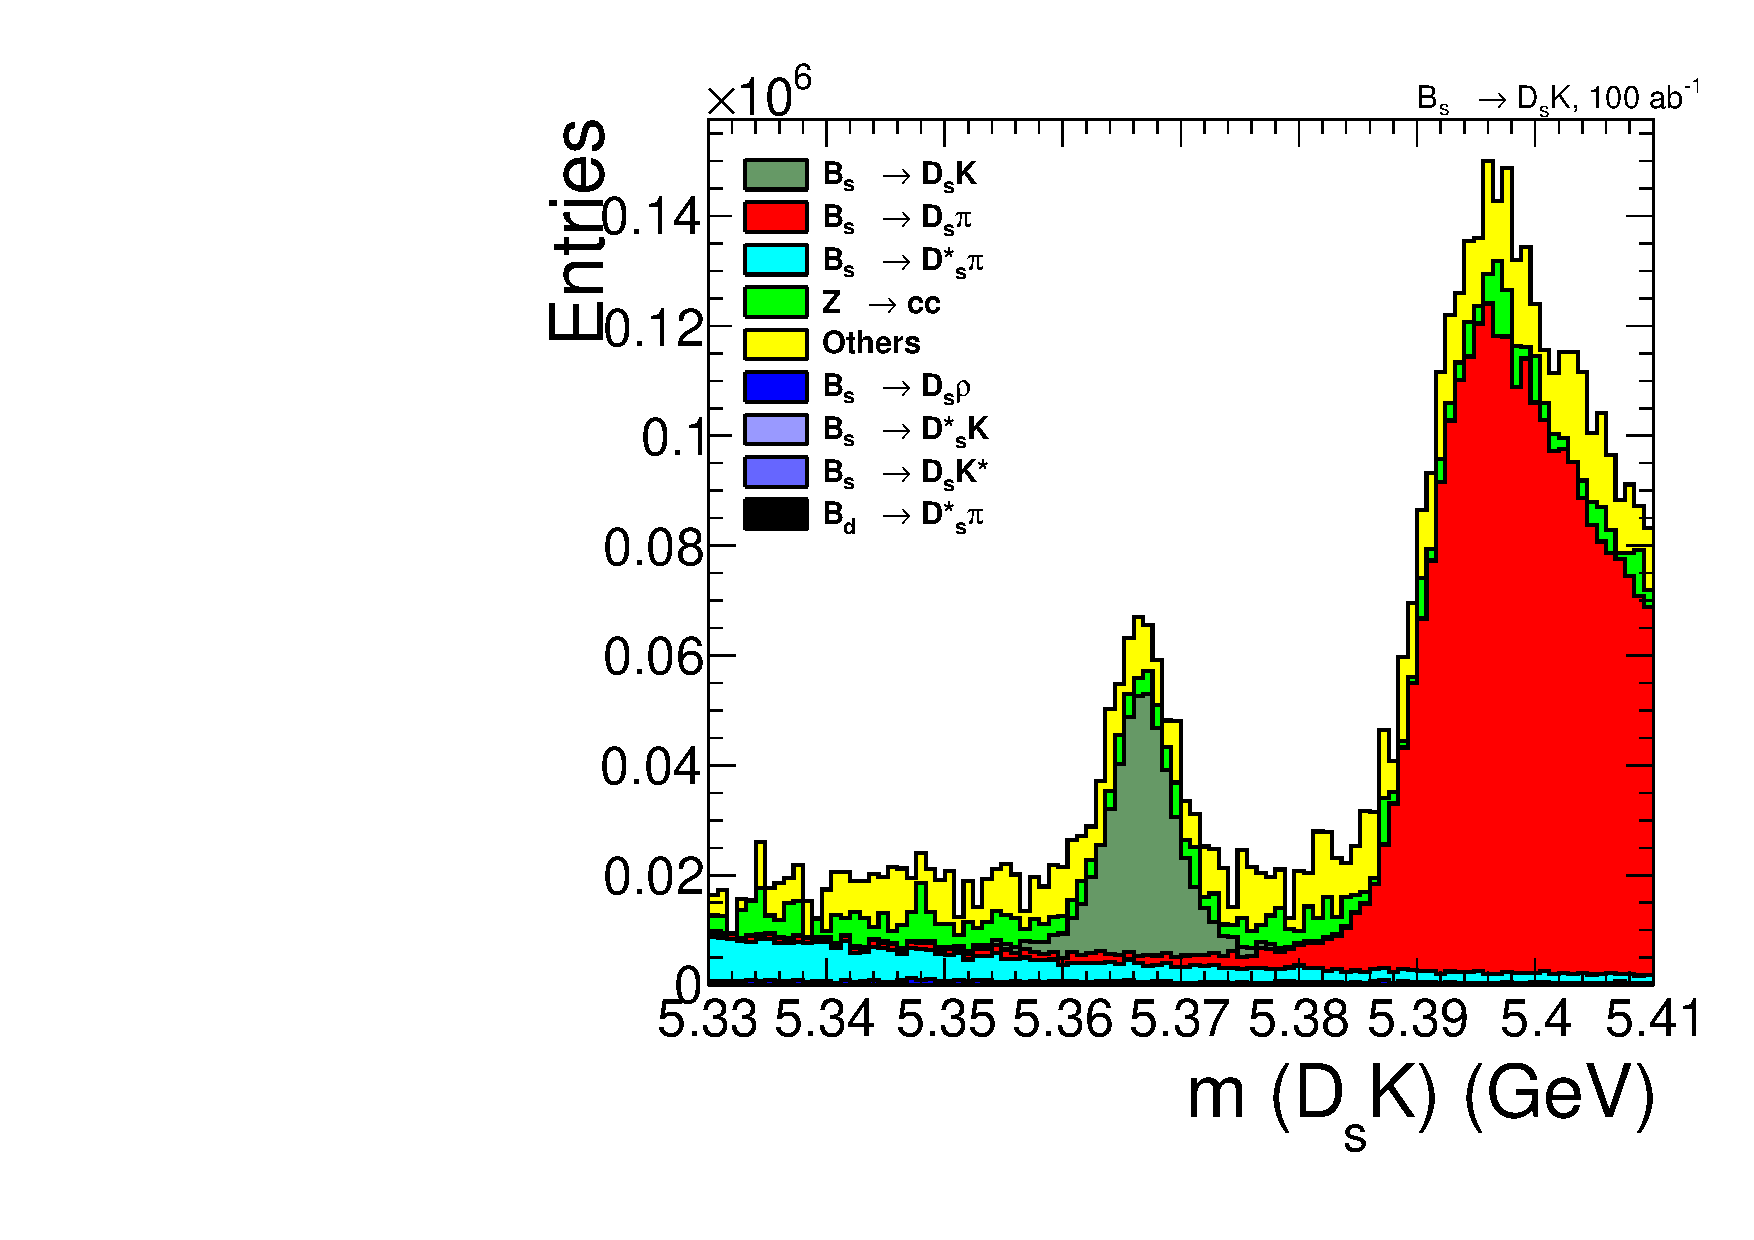
\includegraphics[width=0.49\textwidth]{Physics/DetectorRequirements/Figs/Bs2DsK_pgt1p5_mass_noPID.pdf}
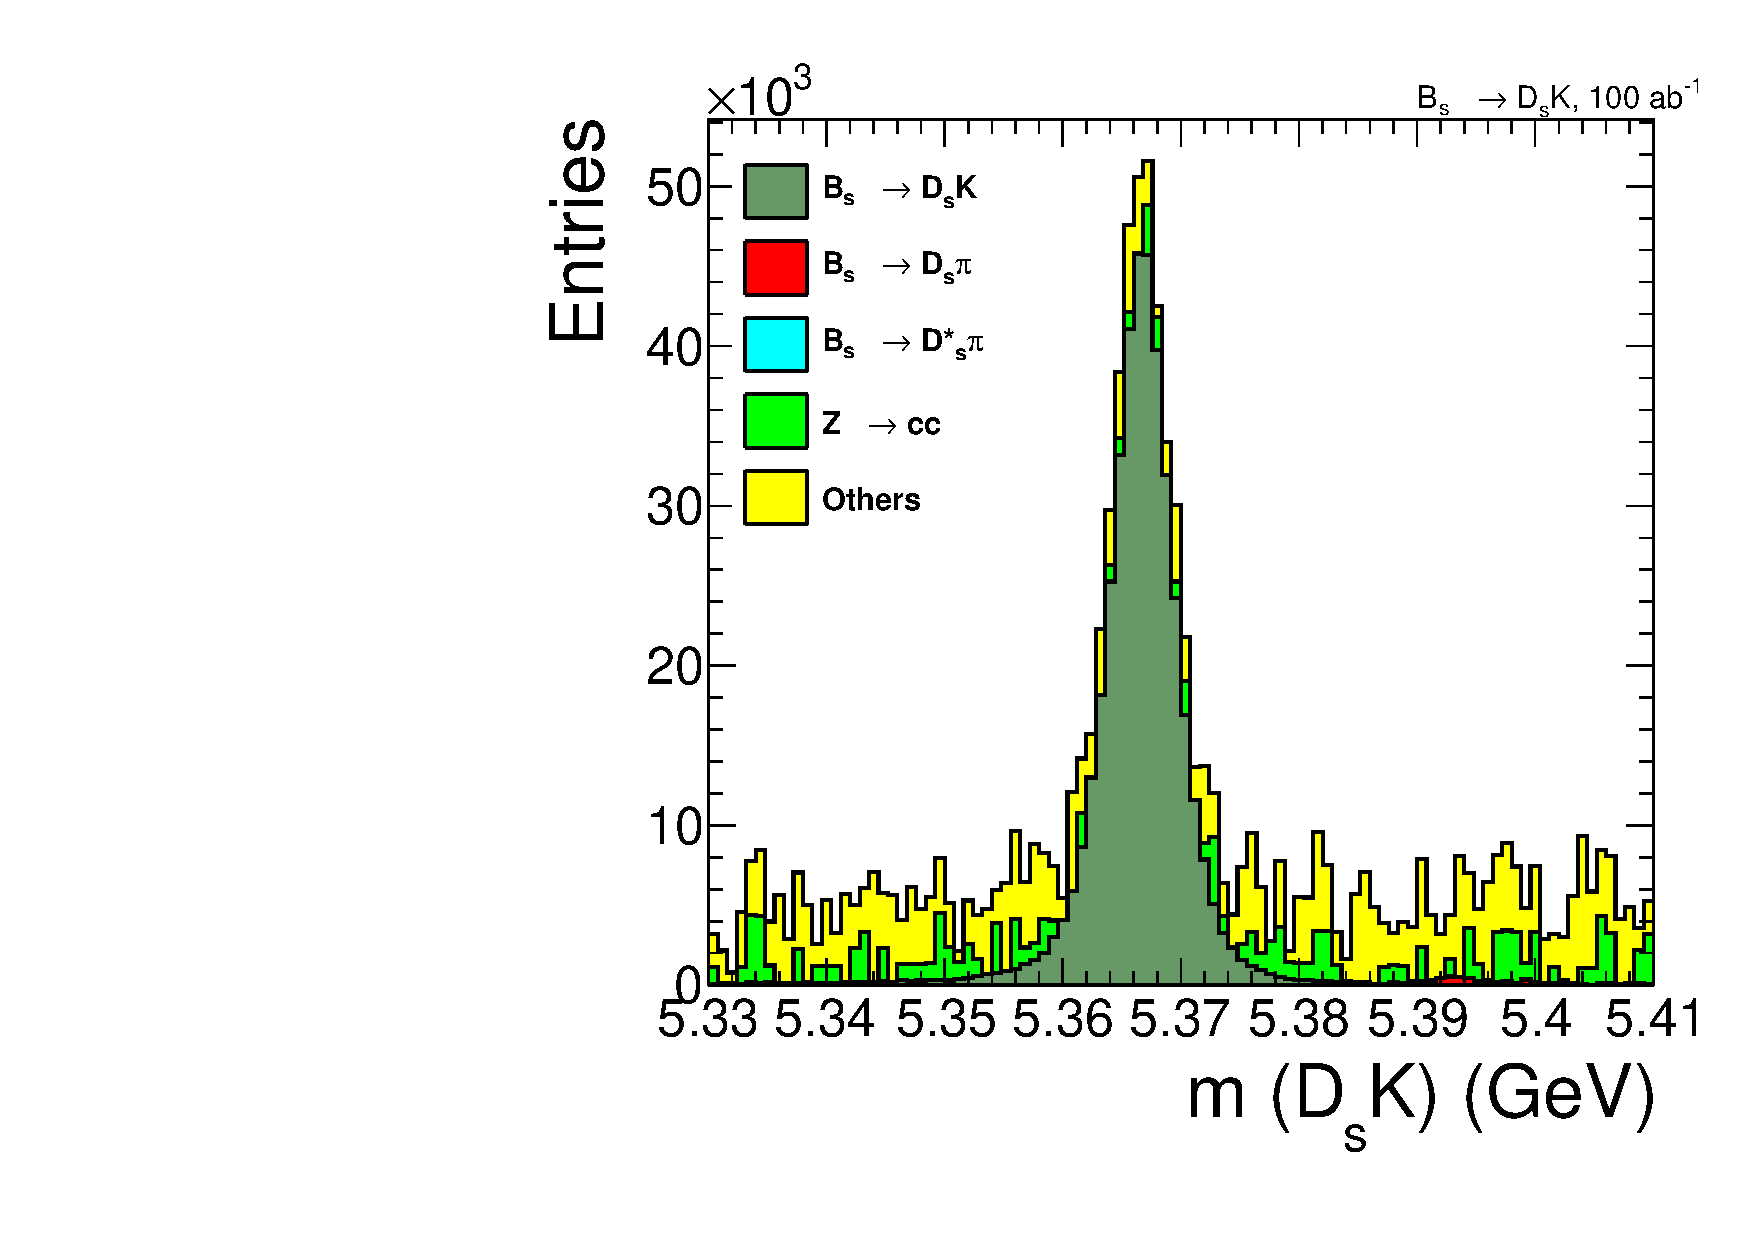
\includegraphics[width=0.49\textwidth]{Physics/DetectorRequirements/Figs/Bs2DsK_pgt1p5_mass_PID.pdf}
\caption{Mass distributions of the \PBs candidates in the $\PBs \to \PDs \PK \to \PGf (\PK\PK) \PGp \PK$ decay channel, 
prior to any PID cut (left) and after requiring that the `bachelor' 
(the particle accompanying the reconstructed \PDs) must be identified as a kaon (right). 
The momentum of the `bachelor' is required to be larger than 1.5\,GeV.}
\label{fig:Bs2DsK}
\end{figure}

The study reported in Ref.~\cite{Aleksan:2021gii}, which considered a few exclusive background processes and used a simple parametrisation of the detector response, 
has been redone for this report with \textsc{Delphes} to simulate the response of the IDEA detector and accounting for the inclusive $\PZ \to \PQb \PAQb$ and $\PZ \to \PQc\PAQc$ backgrounds. 
The analysis starts by exploiting the mass resolution to reconstruct the \PGf candidates and, afterwards, the \PDs candidates, without any PID requirement. 
In a second step, \PBs candidates are built by fitting the \PDs and another track (the `bachelor') to a common vertex~\cite{BedeschiCode}. 
The invariant mass of the \PBs candidates satisfying minimal kinematic and vertex $\chi^2$ cuts is shown in the left panel of Fig.~\ref{fig:Bs2DsK}. 
The signal, shown in dark green, is very well separated from the ten times larger $\PBs \to \PDs \PGp$ background, shown in red. 
However, running the same selection over the inclusive $\PZ \to \PQb\PAQb$ sample shows that there are other sources of backgrounds that contaminate the signal mass peak, 
in addition to the exclusive backgrounds that were considered in Ref.~\cite{Aleksan:2021gii} and that are also shown in Fig.~\ref{fig:Bs2DsK}. 
The right panel of this figure shows that this background is largely suppressed by requiring that the `bachelor' particle must be identified as a kaon, 
which is done by using a PID cut that is 95\% efficient on the signal. 
The PID cut uses the ratio of the likelihoods for the `bachelor' to be a kaon or a pion and combines the d$N$/d$x$ measurement of the track, 
determined with a resolution of about 2\%, and the measurement of its TOF at 2\,m from the interaction point, with a 30\,ps resolution. 
Even for this mode with charged particles only, PID capabilities appear to be mandatory to extract the signal with a decent signal-to-background ratio. 
Since the momentum distribution of the kaons from $\PBs \to \PDs \PK$ decays is hard, time-of-flight measurements alone would not lead to an acceptable background suppression. 
For example, in a mass window that contains 95\% of the reconstructed \PBs candidates (the signal), 
the background contamination decreases from 48\%, without any PID, 
to 33\% if only the TOF measurement is used, 
and to 19\% if both the d$N$/d$x$ and TOF measurements are used (assuming the PID capabilities of IDEA). 
This last value would degrade to 24\% with a twice worse d$N$/d$x$ resolution.

\subsubsection{Work ahead}

\begin{itemize}

\item The measurement of time-dependent CP asymmetries in the \PBs system requires the flavour of the meson (\PBs or \PABs) to be tagged at the time of production. 
Various algorithms are typically combined to achieve this goal. 
A powerful method uses the charge of the kaons in the event that are not associated with the signal decay, which typically have momenta well below 10\,GeV.
The performance of flavour tagging is studied in order to provide requirements on PID at low momentum. 
For example, the determination of the angle $\gamma$ of the CKM matrix, from the $\PBs \to \PDs \PK$ process, 
or of the phase $\beta_s$, from the $\PBs \to \PJGy \, \PGf$ decay, could serve as benchmark measurements. 
The identification of very soft fragmentation kaons (produced when a \PQb (anti-)quark hadronises into a \PBs meson), 
for which the PID performance brought by TOF measurements is relevant, 
should also play a key role in the measurement of the branching fraction of the $\PBs \to \PGn \PAGn$ decay.

\item The determination of $V_{\PQc\PQs}$ from \PW decays may benchmark the performance of strange-quark tagging 
for working points with a much higher purity than that needed for the determination of the coupling of the Higgs boson to the strange quark. 
Alternatively, $V_{\PQc\PQs}$ may be measured in events where exclusive decays of charmed hadrons into kaons are selected, calling for a good $\PGp/\PK$ separation. 
More generally, electroweak measurements involving strange quarks, such as $R_{\PQs}$ or $A_\text{FB}^{\PQs}$, are studied for the requirements on the PID performance.

\item A very precise test of lepton flavour universality in the tau sector is provided by the simultaneous measurements, at the $10^{-5}$ level, 
of the tau lifetime and of the branching fraction of its decay to electrons (Section~\ref{sec:PhysPerf_Taulifetime}). 
The latter requires a $\Pe / \PGp$ separation controlled at the $10^{-5}$ level, 
which might be difficult to achieve from calorimetry measurements alone. 
The requirements on d$E$/d$x$ or d$N$/d$x$ measurements should also be studied in the context of $\Pe / \PGp$ separation.

\end{itemize}

\subsubsection{Preliminary conclusions}

\begin{itemize}

\item It is not only for flavour physics that charged-hadron PID is needed. 
In particular, the potential for constraining the coupling of the Higgs boson to the strange quark provides a strong motivation for having PID, up to high momenta. 
Similarly, powerful strange tagging offers new prospects for electroweak and top measurements in the strange sector, 
such as measurements of the $\PZ \to \PQs \PAQs$ branching fraction~\cite{Blekman:2024wyf} and forward-backward asymmetry,
or of the $V_{\PQt\PQs}$ CKM element via rare $\PQt \to \PW \PQs$ decays~\cite{giappichini_2024_te64m-zbm05}. 

\item The momentum range to be covered, extending from ${\cal{O}}$(150)\,MeV to 40\,GeV, is challenging. 
Current studies show that the $\PGp/\PK$ separation offered by the cluster counting approach, in the IDEA drift chamber, is probably adequate. 
A degradation of the resolution of the energy loss measurement by a factor of 2, with respect to what is expected from the baseline IDEA d$N$/d$x$ performance, 
would have a non-negligible impact on the determination of the Higgs coupling to strange quarks. 
Such a degradation would correspond to the expected d$E$/d$x$ performance.

\item In the absence of specific energy loss measurements in the tracker, 
there is a conceptual design for a compact RICH detector that looks promising and could comfortably cover the required momentum range. 
Detailed simulation studies are needed to evaluate the impact of such a detector on particle-flow reconstruction performance.

\end{itemize}

\subsection{Requirements for electromagnetic calorimetry}
\label{sec:PhysPerf_ECAL}

This section summarises the needs for the measurement of electromagnetic (EM) showers, which may, but does not have to, be performed in a dedicated electromagnetic calorimeter (ECAL).
In the baseline IDEA concept, the EM showers are measured using a finely segmented crystal ECAL with dual readout capabilities~\cite{Lucchini:2020bac}.  
In a variant of this concept, considered in Ref.~\cite{fcc-phys-cdr}, the electromagnetic and hadron showers are both measured in a dual readout (DR) calorimeter that uses scintillation and Cerenkov fibres. 
The CLD concept uses a high-granularity ECAL built as a sandwich of tungsten plates and silicon sensors. 
A high granularity noble liquid ECAL is also under consideration in ALLEGRO. 
These concepts have complementary strengths, ranging from an energy resolution of $\sigma_E / E \simeq 3\% / \sqrt{E}$ for the crystal-based ECAL 
to an extreme transverse resolution of $\sim 2 \times 2$\,mm$^2$ for the fibre DR calorimeter, if each fibre is equipped with a SiPM readout device, 
or to a high longitudinal segmentation for the Si/W or noble liquid solution. 
More details are given in Table~\ref{tab:ECAL_options}. 
The next paragraphs illustrate the requirements on electromagnetic calorimetry from representative analyses. 
Benchmark processes for which the performance is solely driven by the energy resolution are described first, 
followed by one case for which the transverse granularity is crucial, and by examples that place stringent requirements on both the energy resolution and the granularity.

\begin{table}[ht]
\centering
\caption{Expected energy resolution of the different electromagnetic calorimeter options considered in the studies of Ref.~\cite{Aleksa:2021ztd}.}
\label{tab:ECAL_options}
\begin{tabular}{l c c  c }
\toprule
        Technology & \multicolumn{2}{c}{EM energy resolution}\\
                   & stochastic term  & constant term       \\   
\midrule
        Highly granular Si/W based & 15--17\% & 1\% \\
        Dual readout fibre (ECAL$+$HCAL)  & 11\% & $<1$\%  \\
        Hybrid crystal (dual readout) &  3\% &  $<1$\%  \\
        Highly granular noble liquid based ECAL  & 8--10\% & $<1$\% \\
\bottomrule
\end{tabular}
\end{table}

\subsubsection{Energy resolution and monophoton final states}

For final states that consist of a single photon and nothing else in the detector, the main handle to suppress the backgrounds is the electromagnetic energy resolution.
Two physics cases have been considered for such final states: 
the determination of the $\PZ \PGne \PAGne$ coupling and the search for long-lived axion-like particles.

\paragraph{Measurement of the \texorpdfstring{\PZ}{Z} coupling to the \texorpdfstring{\PGne}{nu-e}}

As described in Ref.~\cite{Aleksan_2019}, the $\epem \to \PGne \PAGne \PGg$ process at FCC-ee can be used to improve the precision measurement of the poorly known coupling of the \PZ to the \PGne, 
currently known as $g^{\PGne}_{\PZ} = 1.06\pm 0.18$~\cite{ParticleDataGroup:2024cfk}.
This is possible because of the presence of the $t$-channel \PW exchange in the $\epem \to \PGne \PAGne \PGg$ process, interfering with $\epem \to \PZ(\PGne \PAGne) \PGg$. 
This interference slightly deforms the distribution of the missing mass $M_{\PGn \PAGn}$ (or, equivalently, of the photon energy) in the vicinity of the resonant peak, $M_{\PGn \PAGn} = M_{\PZ}$, 
increasing (decreasing) the cross section above (below) the mass peak.
The measurement is based on the asymmetry $A_s$ of the photon energy spectrum in an interval of about $\pm 1$\,GeV around the peak 
(where the photon energy is approximately equal to $\sqrt{s}/2 \times (1 - M^2_{\PZ} / s)$, i.e.\ 54\,GeV at $\sqrt{s} = 161$\,GeV)
using event samples generated with the \textsc{kkmc}~\cite{Arbuzov:2020coe,Arbuzov_2021} matrix element MC generator.   
At the $\PW\PW$ threshold, with an integrated luminosity of 10\,ab$^{-1}$ and without considering any detector effects, 
this asymmetry would be measured with a statistical uncertainty of $2 \times 10^{-4}$, which translates into a 1\%  statistical uncertainty on $g^{\PGne}_{\PZ}$, 
as shown on the left panel of Fig.~\ref{fig:nunugamma}.

\begin{figure}[ht]
\centering
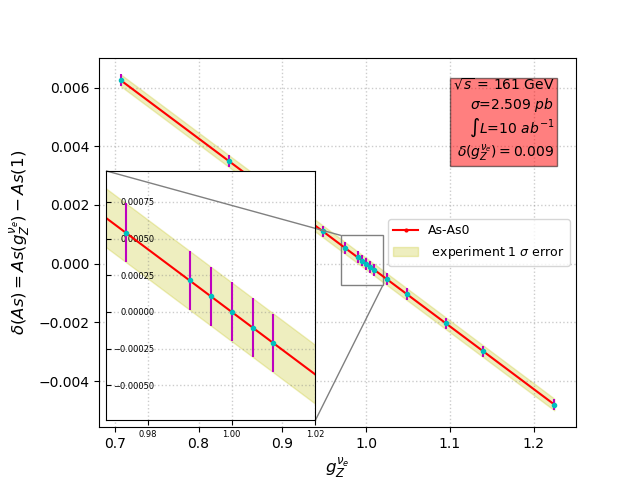
\includegraphics[width=0.495\textwidth]{DetectorRequirements/ECALFIG/g_nue_sensitivity-161GeV_zoom.png} 
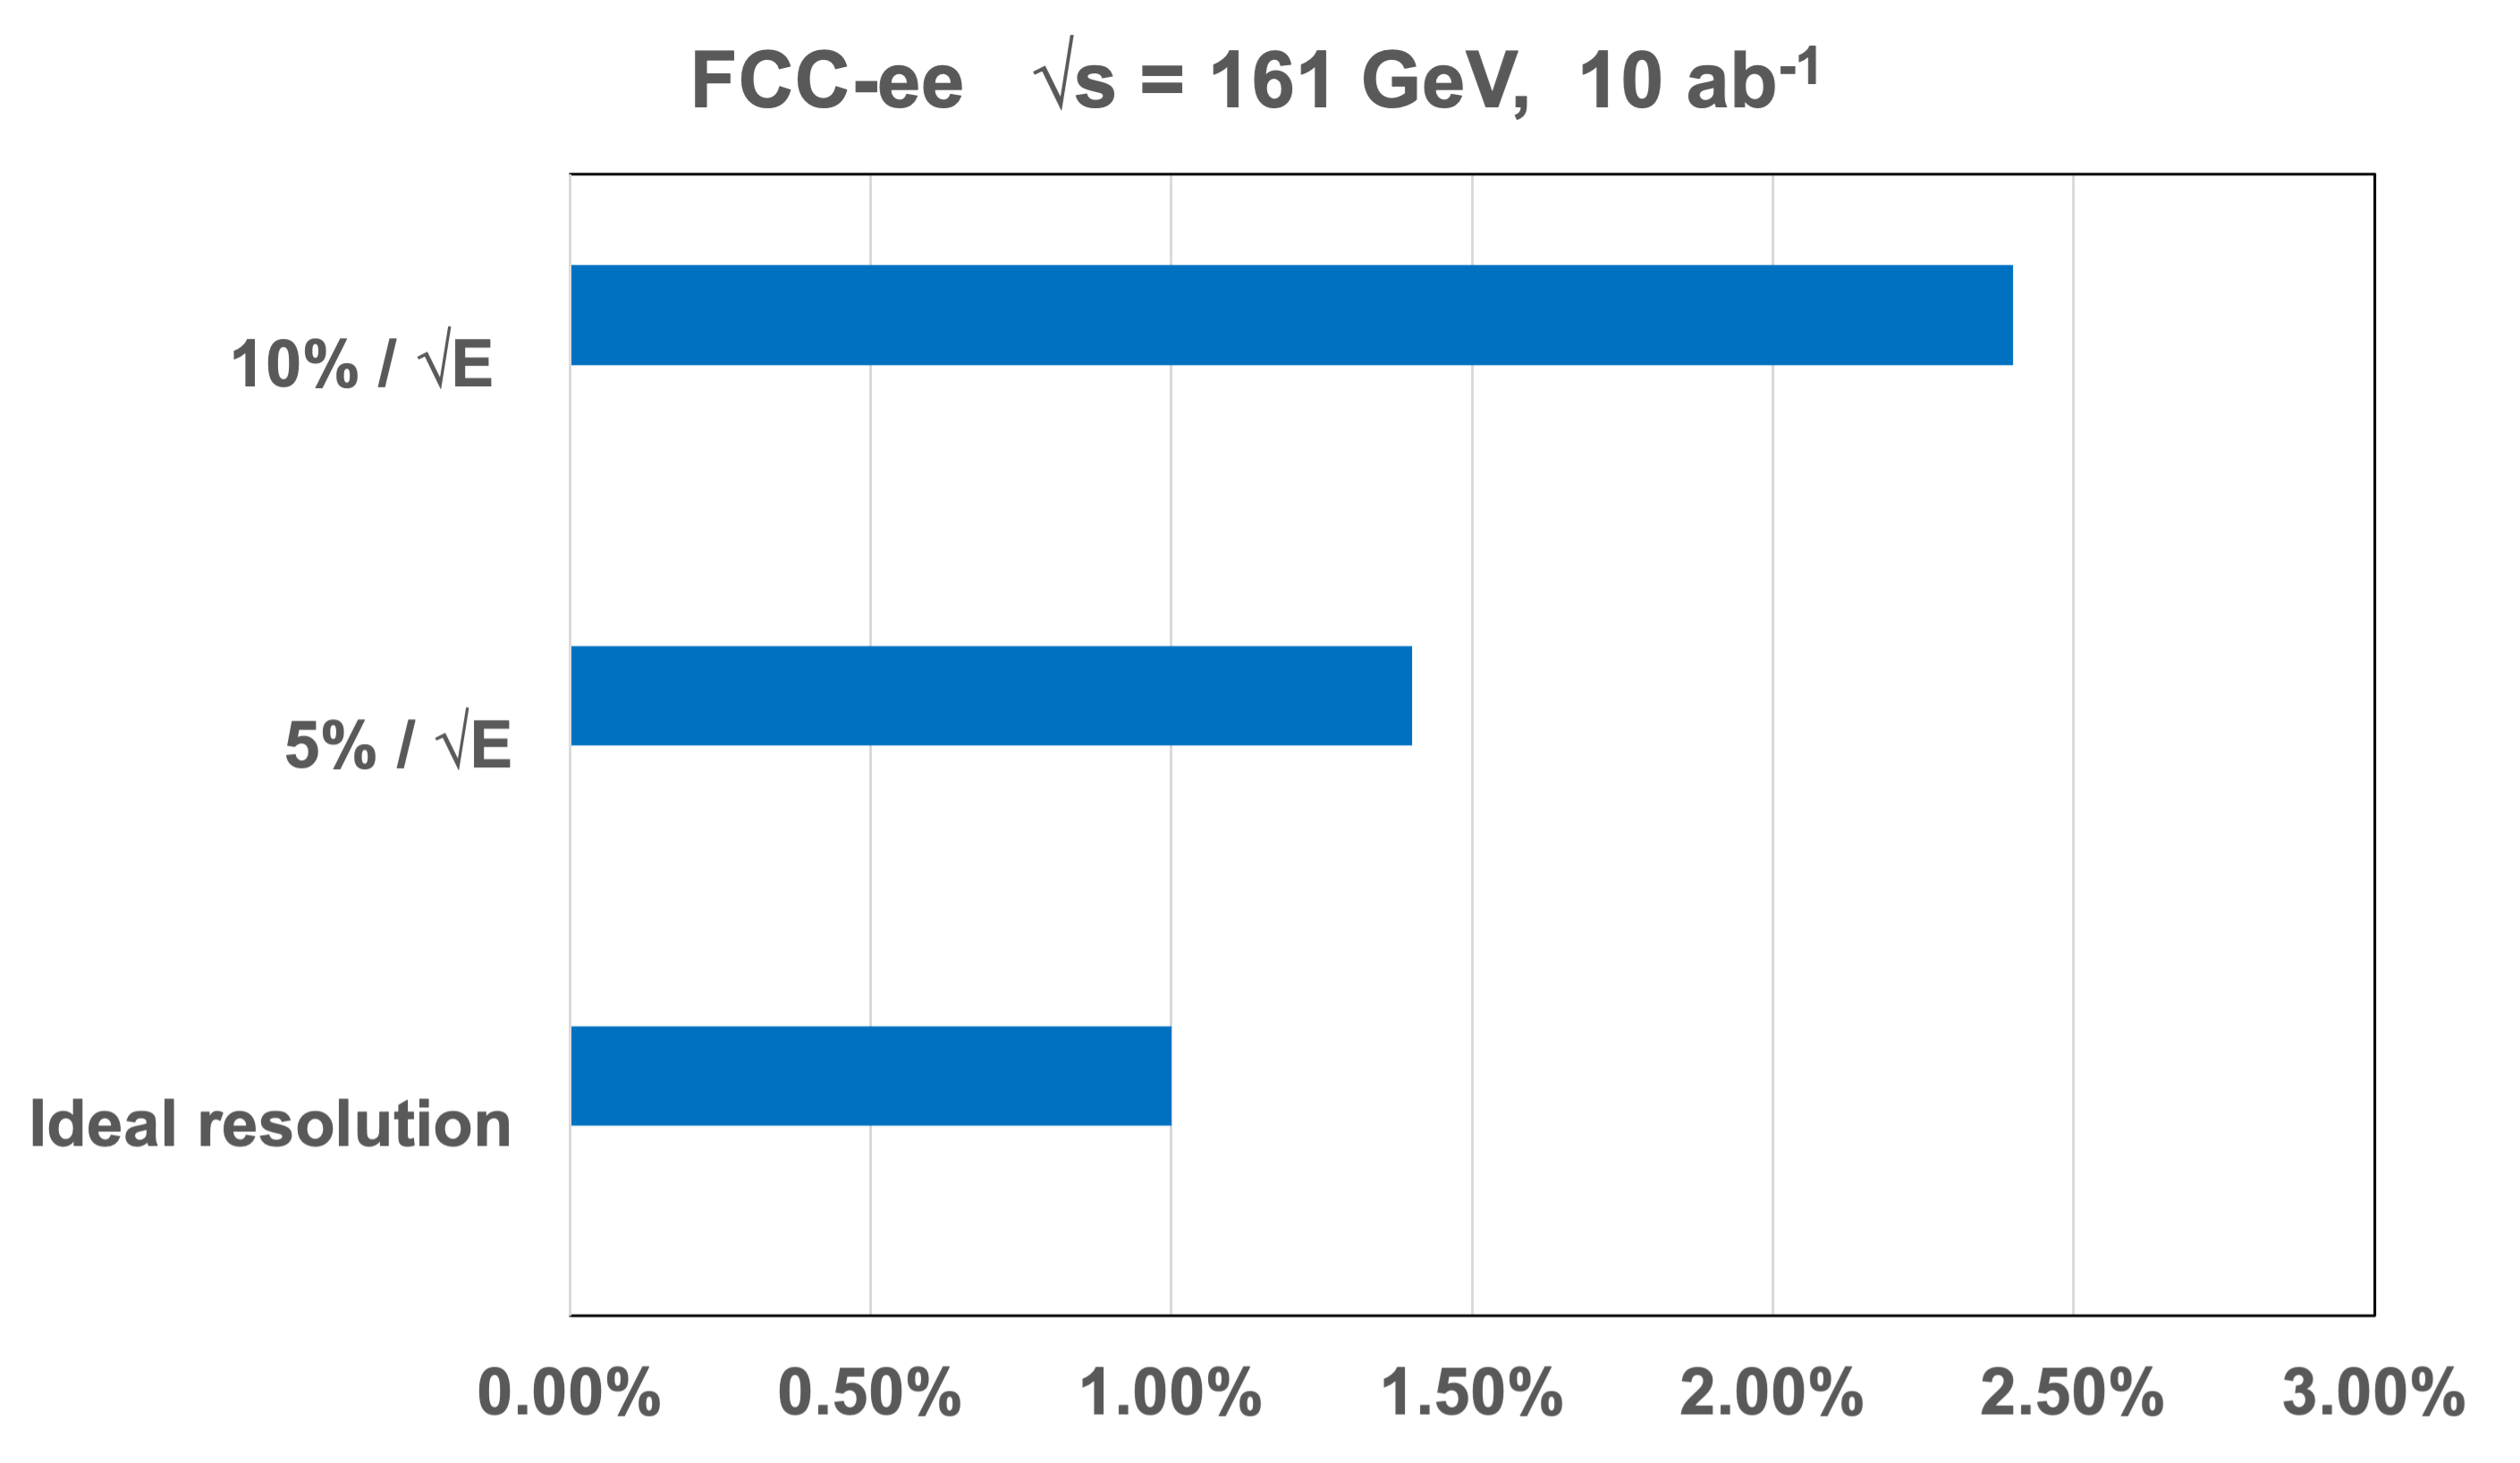
\includegraphics[width=0.495\textwidth]{Physics/DetectorRequirements/Figs/Znuenue_summary.png}
\caption{Left: Asymmetry $A_s$ of the photon energy spectrum, at the $\PW\PW$ threshold and without detector effects,
after subtracting the SM asymmetry predicted for $g^{\PGne}_{\PZ} = 1$, as a function of the coupling. 
The yellow band represents the statistical uncertainty expected with an integrated luminosity of $10$\,ab$^{-1}$. 
Illustrative measurement points along the prediction, with error bars that span the uncertainty band, are also shown. 
Right: Statistical uncertainty on the coupling $g^{\PGne}_{\PZ}$ expected at the $\PW\PW$ threshold, 
for two example values of the stochastic term of the electromagnetic energy resolution (with a constant term of 0.2\% added in quadrature). 
The uncertainty that would be obtained with a perfect detector is also shown.}
\label{fig:nunugamma}
\end{figure}

To evaluate the impact of a more realistic detector, 
the study was redone including the resolution from a homogeneous calorimeter with an energy resolution of $\sigma(E_{\PGg})\,/\,E_{\PGg} = 0.05/\sqrt{E_{\PGg}} \,\oplus\, 0.002$, 
resulting in a 50\% degradation of the sensitivity to 1.4\%, which remains an excellent performance. 
Should the stochastic term be two times larger (i.e., $0.1/\sqrt{E}$, a value typical for a sampling calorimeter) the sensitivity would degrade to 2.4\%. 
The right panel of Fig.~\ref{fig:nunugamma} summarises the expected uncertainties. 
This study brings a clear constraint on the need for a very good calorimeter energy resolution and knowledge of photon energy calibration, 
to keep the uncertainty due to the calorimeter resolution at the per-cent level, as expected with a perfect detector.

\paragraph{Search for long-lived ALPs that decay outside the detector}

Very long-lived axion-like particles (ALPs) could be copiously produced at Tera-\PZ in \PZ decays 
($\epem \to \PZ / \PGg^{*} \to \axion + \PGg$). 
When the ALP $\axion$ decays outside the detector, the final state consists in a (monochromatic) single photon, with nothing else in the detector. 
The relevant mass range for such long-lived ALPs being below ${\cal{O}}$(1)\,GeV, the photon energy is about 45\,GeV.  
The sensitivity of FCC-ee to such particles has been studied in Ref.~\cite{note_ALP_Polesello}. 
Simple kinematic cuts allow the reducible background 
(dominated by the associated production of a photon with two fermions that escape detection) 
to be fully eliminated. 
Since the irreducible background due to $\epem \to \PGn \PAGn \PGg$ production 
rises very steeply when the photon energy decreases, 
the ECAL energy resolution is a key driver of the experimental sensitivity. 
Figure~\ref{fig:PhysPerf_ALPs_monophotons} shows the 2\,$\sigma$ sensitivities expected for a crystal-based ECAL 
and for a dual-readout calorimeter, the former allowing  significantly lower values of the ALP coupling to be probed. 
As was shown in Fig.~\ref{fig:axion}, this analysis would uniquely cover the range between $\lesssim$\,0.1 and $\sim$\,1\,GeV, 
which is beyond the reach of beam dump experiments.

\begin{figure}[ht]
\centering
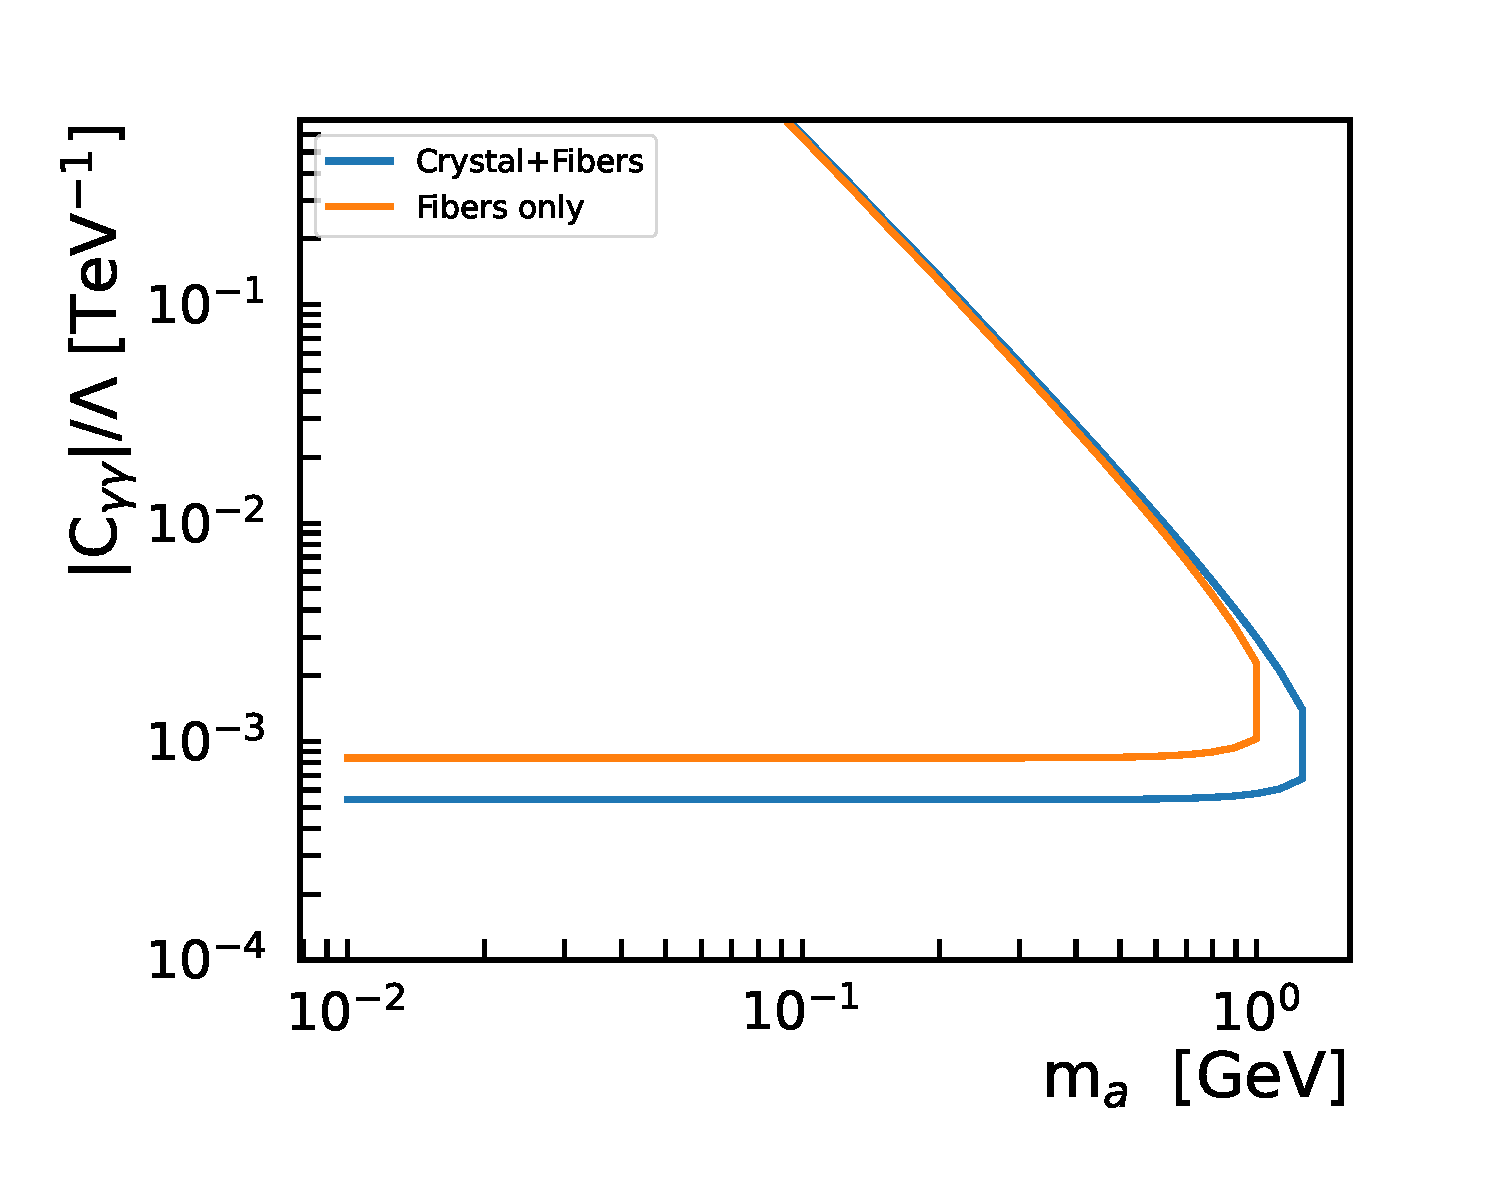
\includegraphics[width=0.55\textwidth]{Physics/DetectorRequirements/Figs/ALPs_mono2calo.pdf}
\caption{Expected sensitivity, at the 2\,$\sigma$ level, of an FCC-ee experiment with a relative EM energy resolution 
of $3\% / \sqrt{E}$ (blue curve) or $14\% / \sqrt{E}$ (orange curve), in the parameter space spanned by the mass of the ALP and its coupling to two photons, 
from a search in the monophoton final state~\cite{note_ALP_Polesello}.}
\label{fig:PhysPerf_ALPs_monophotons}
\end{figure}

\subsubsection{Energy resolution and decays of heavy flavoured hadrons into photons or \texorpdfstring{\PGpz}s}
\label{sec:PhysPerf:pi0_reco_for_flavour}

The FCC-ee flavour programme at the \PZ pole significantly expands beyond that of Belle~II and LHCb, as described in Ref.~\cite{Monteil:2021ith}. 
In particular, for all decay modes common to the \PBs and the \PBd mesons, and that involve neutral particles, 
the \PBd decays constitute an irreducible background to the \PBs signal. 
In that case, the mass resolution, driven by the electromagnetic calorimeter resolution, is the only handle to separate them.
Two examples have been looked into: 
the radiative decay of $\PB_{(\PQs)}$ into $\PK^* \PGg$ and the $\PBs \to \PDs \PK$ decay where the \PDs decays into $\PGf \PGr$.

\begin{figure}[ht]
\centering
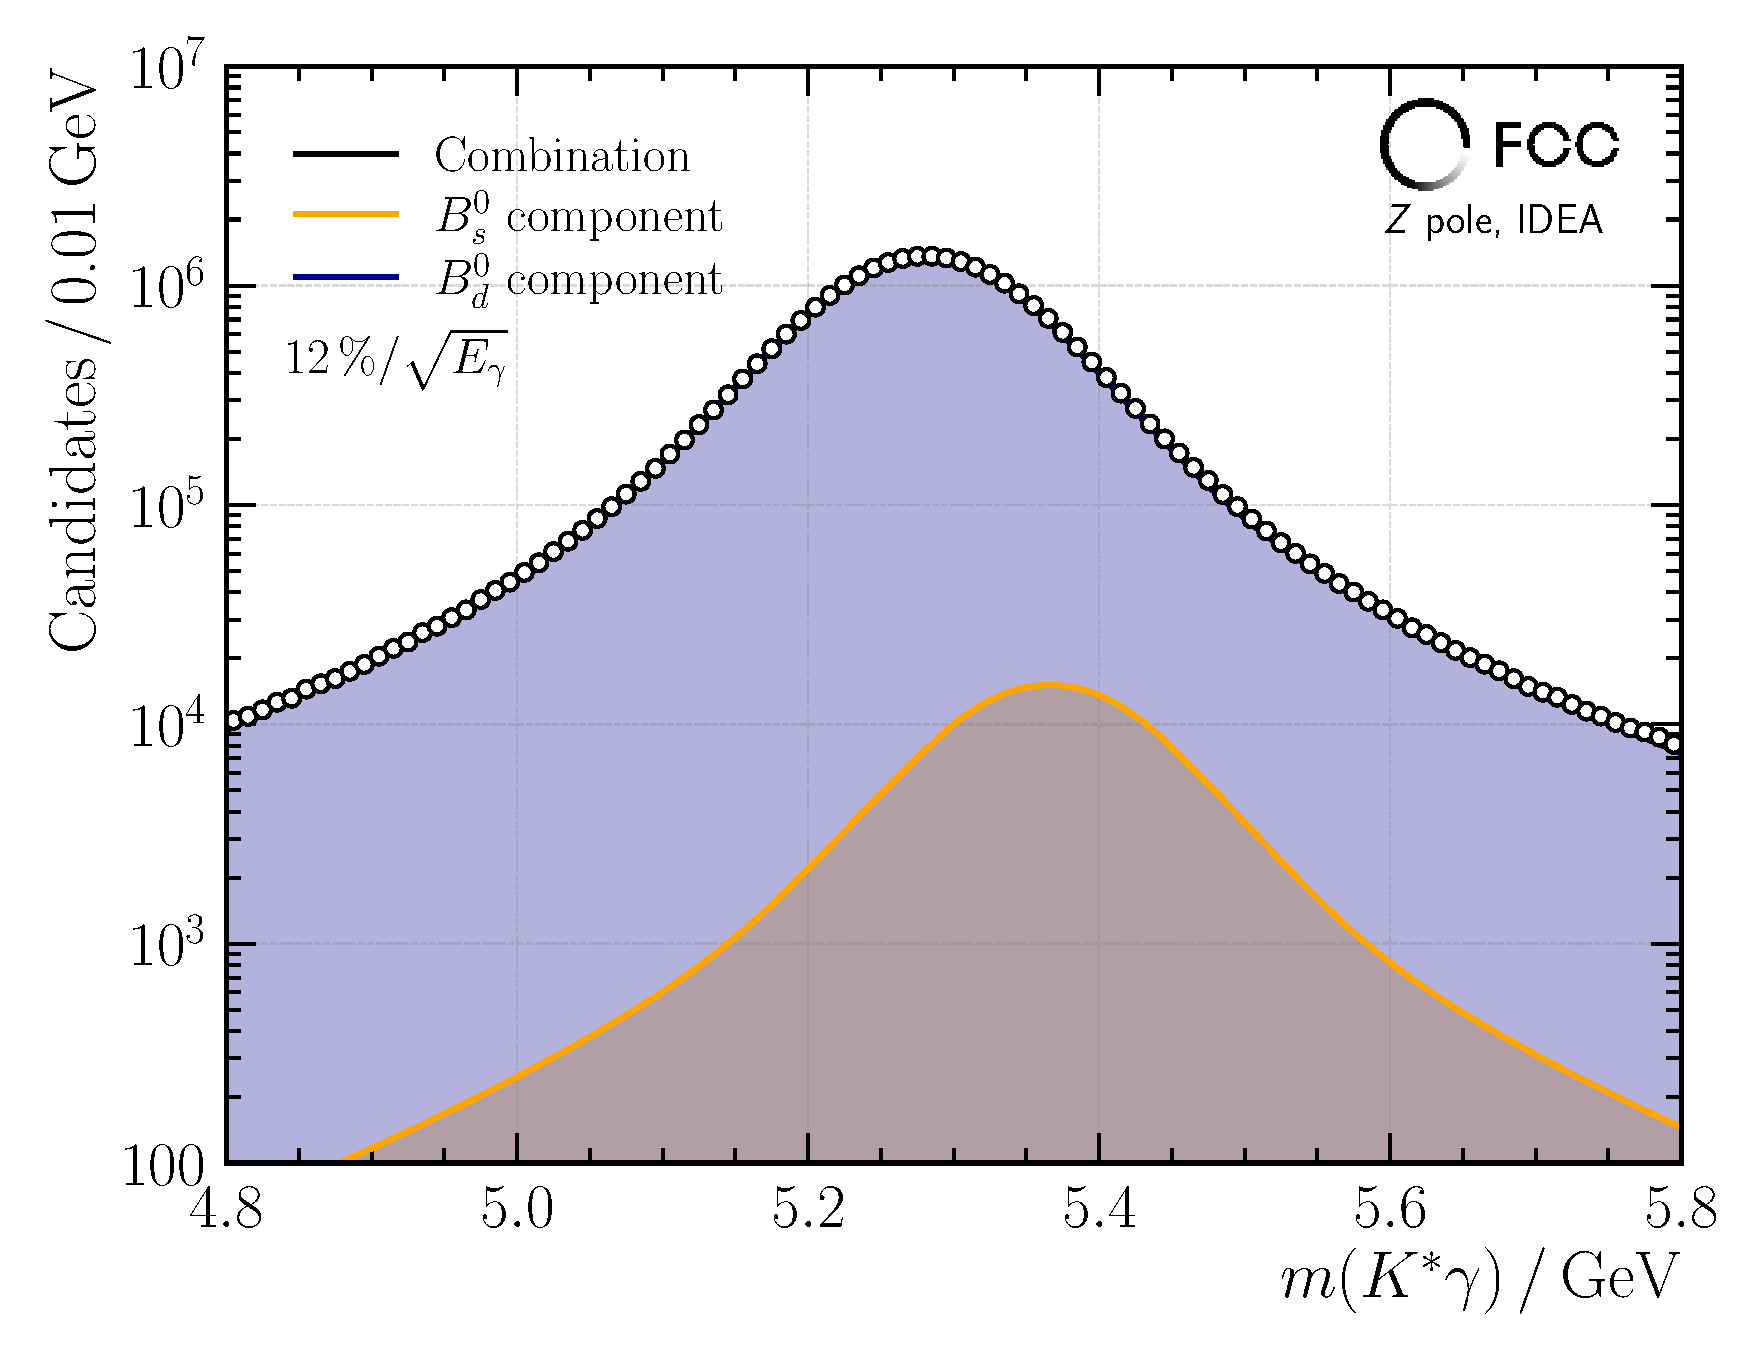
\includegraphics[width=0.45\textwidth]{Physics/DetectorRequirements/Figs/KstarGamma_B0_Bs_separation_012.pdf}
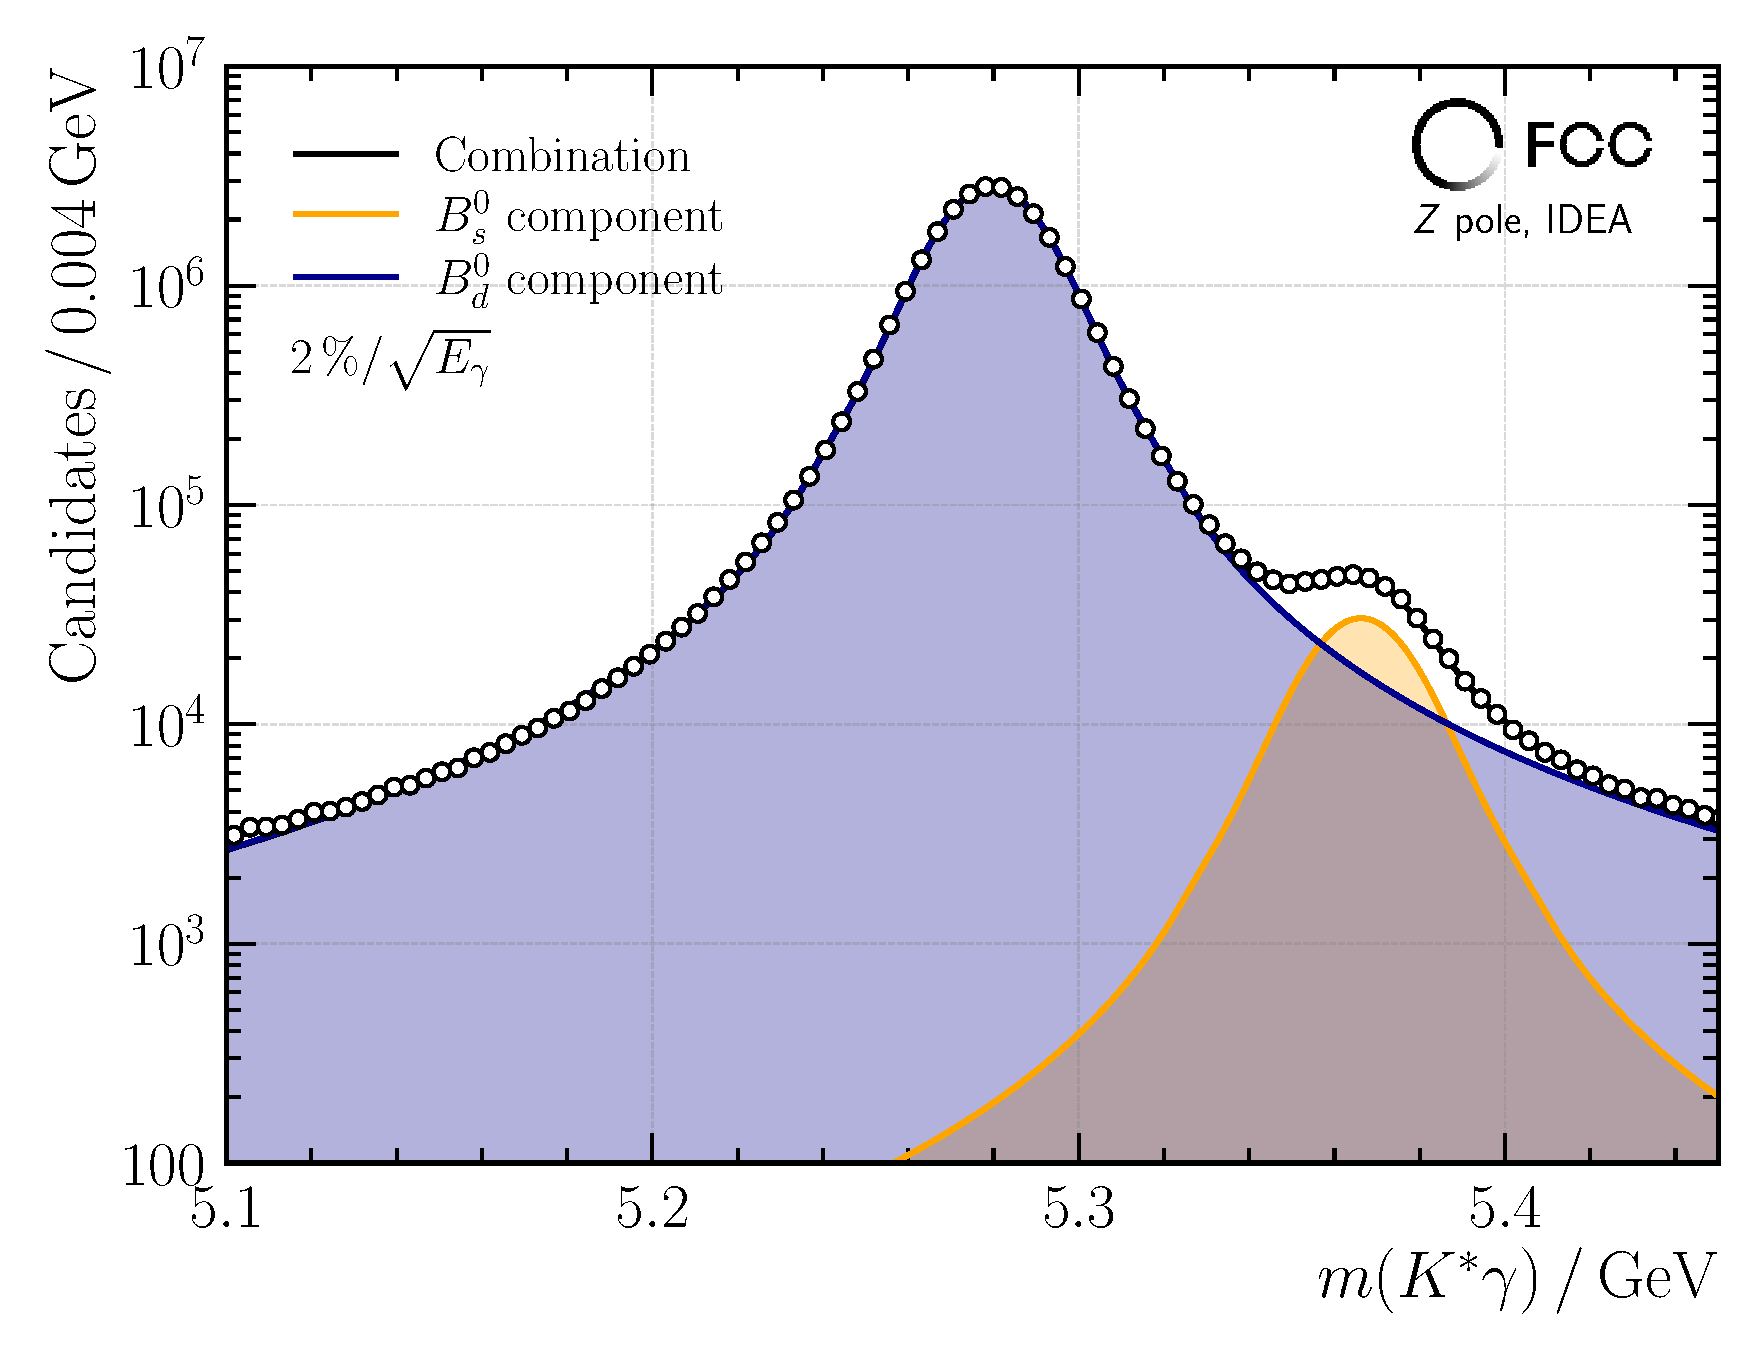
\includegraphics[width=0.45\textwidth]{Physics/DetectorRequirements/Figs/KstarGamma_B0_Bs_separation_002.pdf}
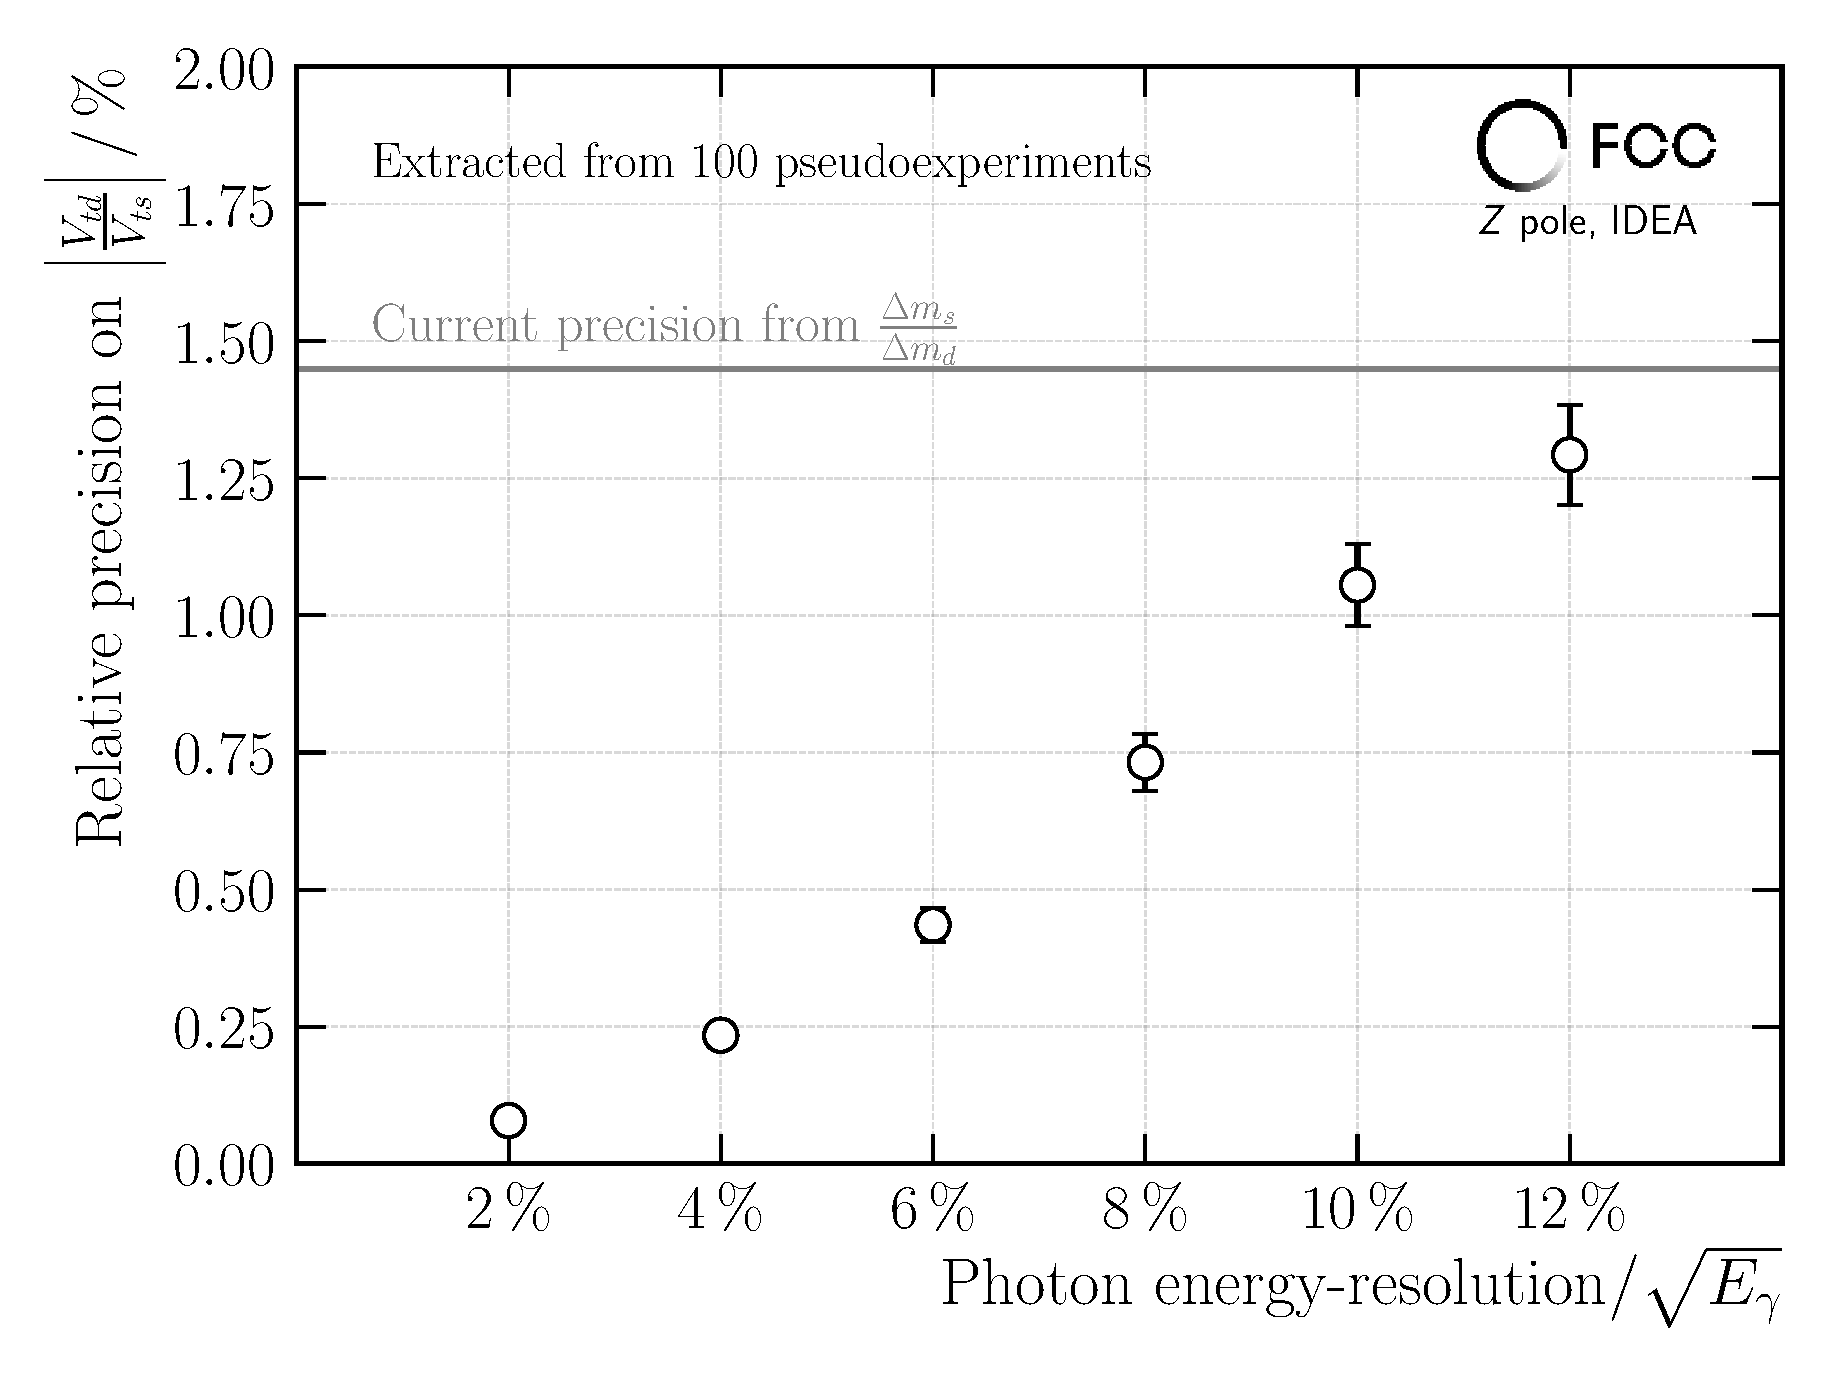
\includegraphics[width=0.45\textwidth]{Physics/DetectorRequirements/Figs/KstarGamma_Relative_Vts_Vtd_squared_ECAL_resolution_with_current_and_without_fit_FCCee_stat}
\caption{Top: Mass distribution of \PB mesons decaying into $\PK^* \PGg$ with an electromagnetic energy resolution 
of $12\% / \sqrt{E}$ (left) or $2\% / \sqrt{E}$ (right). 
Bottom: Relative uncertainty on $|V_{\PQt\PQs} / V_{\PQt\PQd}|$ expected from the measurement of the ratio of the two branching fractions, 
as a function of the stochastic term of the EM energy resolution. The current uncertainty is shown by the horizontal line.}
\label{fig:KstarGamma}
\end{figure}

\paragraph{The radiative decay of the \texorpdfstring{$\PB_{(\PQs)}$}{Bs} meson to \texorpdfstring{$\PK^* \PGg$}{K* gamma}}

Radiative decays, such as $\PBd \to \PK^* \PGg$ ($\PQb \to \PQs \PGg$) and $\PBs \to  \PK^* \PGg$ ($\PQb \to \PQd \PGg$), 
are a sensitive probe for physics beyond the SM and can be used to place complementary constraints on the unitarity triangle.
The yet unobserved $\PBs \to \PK^* \PGg$ decay is an example of $\PQb \to \PQd$ transitions that 
an experiment at a high-luminosity \PZ factory can probably uniquely study, 
provided that it can benefit from a precise photon-energy measurement complementing an excellent reconstruction of displaced vertices.
A first study of the FCC potential to observe this decay has been reported in Ref.~\cite{note_KstarGamma}. 
It assumes perfect charged hadron particle and photon identifications and ignores background contributions.
The reconstructed charged kaon and pion corresponding to the $\PK^* \to \PK \PGp$ decay 
are combined with the generated photon (the energy of which is smeared to account for the detector resolution).
The \PBs signal yield is estimated from the CKM matrix elements and the corresponding hadronisation fractions $f_{\PQd}$ and $f_{\PQs}$, 
leading to the ratio $N_{\PBd} / N_{\PBs} \sim 92$.
The distribution of the resulting ${\PK}^\ast \PGg$ invariant mass is shown in Fig.~\ref{fig:KstarGamma} 
for two values of the stochastic term of the electromagnetic energy resolution.
A sufficiently-high photon-energy resolution is mandatory for the peak of the \PBs signal to become visible 
and distinguishable from the overwhelming $\rm B^0_d$ counterpart spectrum. 
With a stochastic term of 2\%, the ratio of the two  branching fractions could be extracted with a relative statistical uncertainty better than 0.1\%. Provided that the ratio of the form factors of the two decays is well known, 
this opens the way to a very precise direct measurement of the $|V_{\PQt\PQd} / V_{\PQt\PQs}|$ ratio, as shown in the bottom plot of Fig.~\ref{fig:KstarGamma}.
A measurement may still be possible with a resolution of $12 \% / \sqrt{E}$, 
but that would require an excellent control of the shapes of the mass distributions, 
in particular of the tails (assumed here to be perfectly known), 
and the precision would anyway degrade by at least an order of magnitude.

\paragraph{The \texorpdfstring{$\PBs \to \PDs \PK$}{Bs to Ds K} decay}

The copious \PBs decay modes to neutral particles are inaccessible at Belle~II and challenging at LHCb, and can be uniquely studied at FCC-ee. 
A few benchmark studies have been performed to extract the necessary detector requirements for PID (Section~\ref{sec:PhysPerf_PID}) and calorimetry. 
One of them is the study of the $\PBs \to \PDs \PK$ decay~\cite{AleksanFCCPhys4}, 
where the \PDs decays via $\PDps \to \PGf\PGr \to \PKp\PKm \PGpp\PGpz$, 
which could increase the size of the \PBs sample by a factor of 3 with respect to that obtained with the single mode studied in Section~\ref{sec:PhysPerf_PID}. 
Figure~\ref{fig:BsDsK} shows the impact on the mass resolution of the \PBs system when a crystal-like calorimeter is employed, 
improving the resolution of the calorimeter 
from $\sigma_E\,/\,E = 0.15/\sqrt{E} \,\oplus\, 0.005$, corresponding to a resolution of 51\,MeV, 
to $\sigma_E\,/\,E = 0.03/\sqrt{E} \,\oplus\, 0.005$, corresponding to 14\,MeV.

\begin{figure}[ht]
\centering
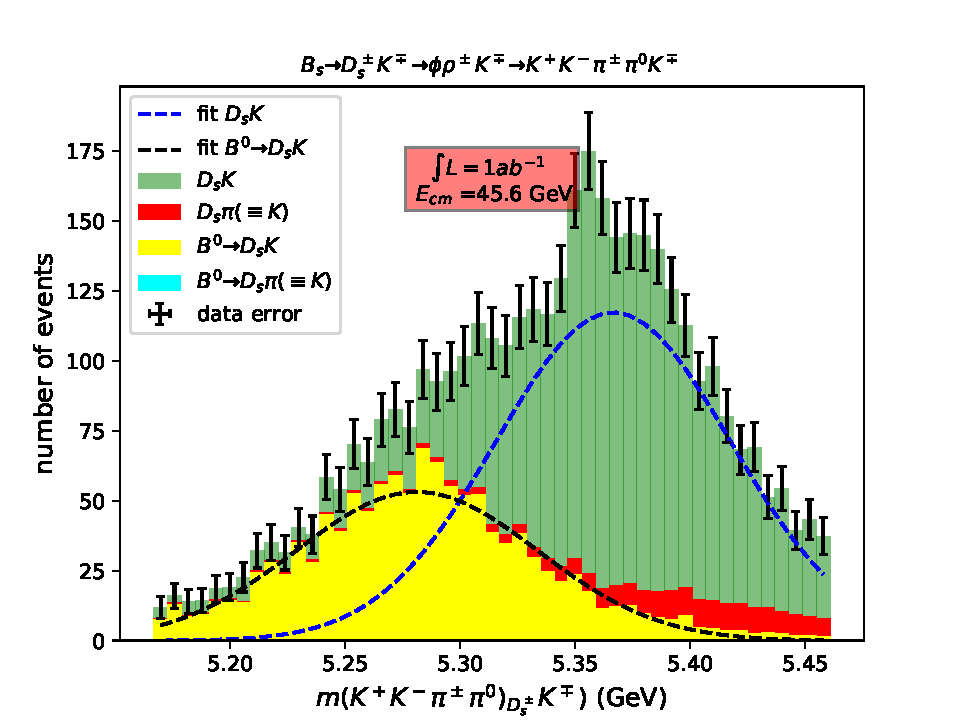
\includegraphics[width=0.495\textwidth]{DetectorRequirements/ECALFIG/DsK_phi-rho-K_HGCAL_notext.pdf} 
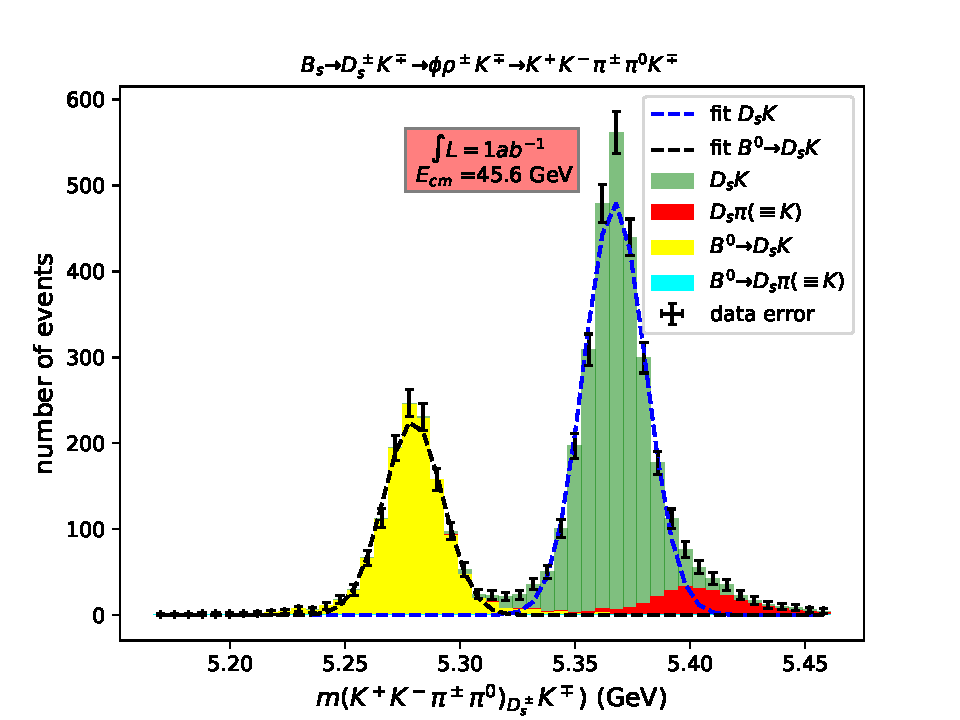
\includegraphics[width=0.495\textwidth]{DetectorRequirements/ECALFIG/DsK_phi-rho-K_HXtal_notext.pdf} 
\caption{Distribution of the mass of the reconstructed \PBs system (in GeV) for the process $\PBs \to \PDs \PK \to \PGf\PGr \PK \to \PK\PK \PGp\PGpz \PK$, 
on top of the main backgrounds, for a calorimeter with an energy resolution of $15\% / \sqrt{E}$ (left) or $3\% / \sqrt{E}$ (right). 
PID is included. 
The resolution on the photon angles has a negligible effect on the resolution of the mass of the \PBs candidates.}
\label{fig:BsDsK}
\end{figure}

\subsubsection{Requirements on the geometrical acceptance for 
\texorpdfstring{$\epem \to \PGg\PGg$}{e+e- to gamma gamma} and \texorpdfstring{$\ell^+\ell^-$}{ell+ ell-} events at \texorpdfstring{\PZ}{Z}-pole energies}
\label{sec:PhysPerf_gammagamma}

The determination of the \PZ lineshape parameters requires the measurement of the hadron and lepton cross sections at and around the \PZ pole. 
With $1.5 \times 10^{12}$ \PZ bosons produced at each FCC-ee interaction point, statistical precisions of ${\cal{O}}$($10^{-6}$) are within reach. 
Critical limiting uncertainties come from the counting of lepton pairs ($\epem \to \ell^+\ell^-$, with $\ell = \PGm$, \PGt) 
and from the integrated luminosity measurement. 
At \mbox{FCC-ee}, the wide-angle diphoton process $\epem \to \PGg\PGg$ becomes statistically relevant and offers prospects for a safer determination 
(in terms of systematic uncertainties) of the integrated luminosity than the traditional low-angle Bhabha scattering, $\epem \to \epem$.

\begin{figure}[ht]
\centering
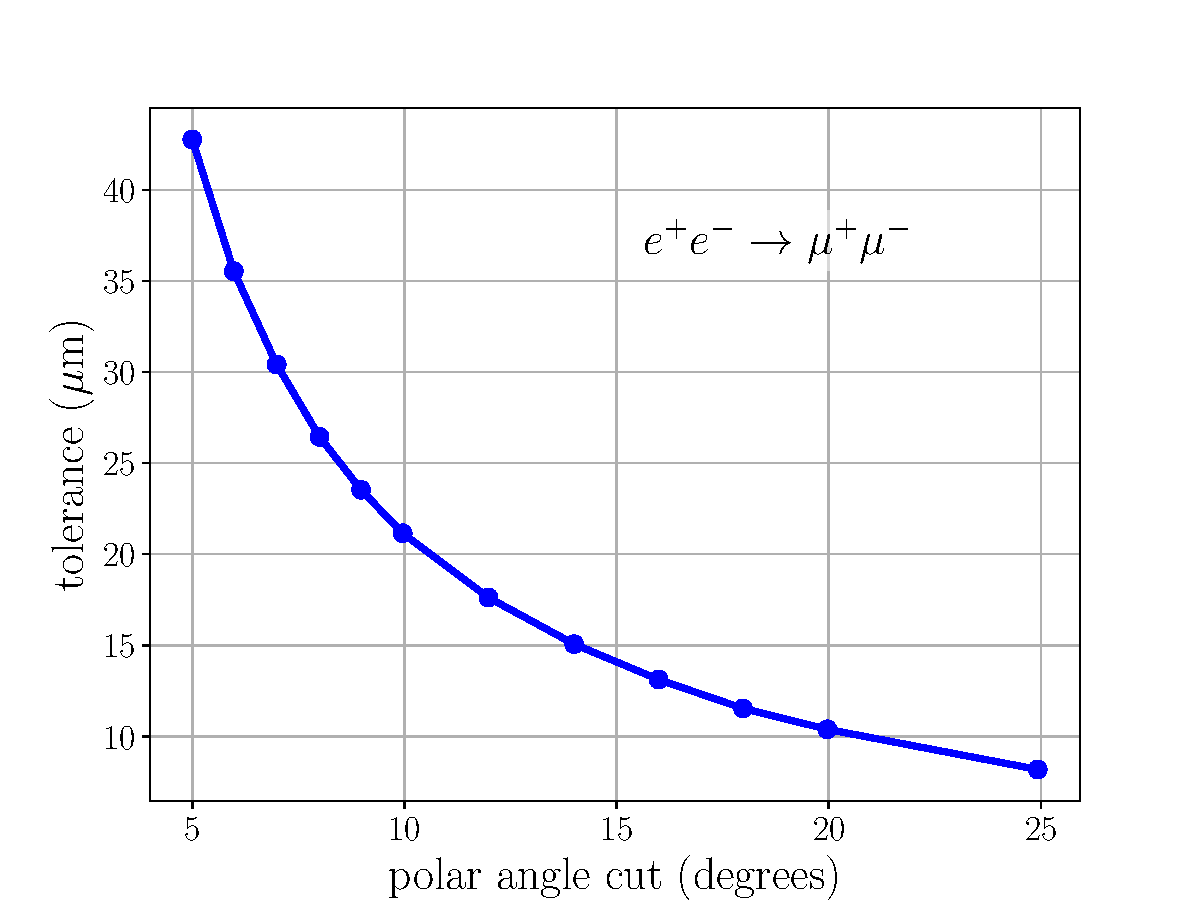
\includegraphics[width=0.50\textwidth]{DetectorRequirements/ECALFIG/DiMuonTolerance.pdf}
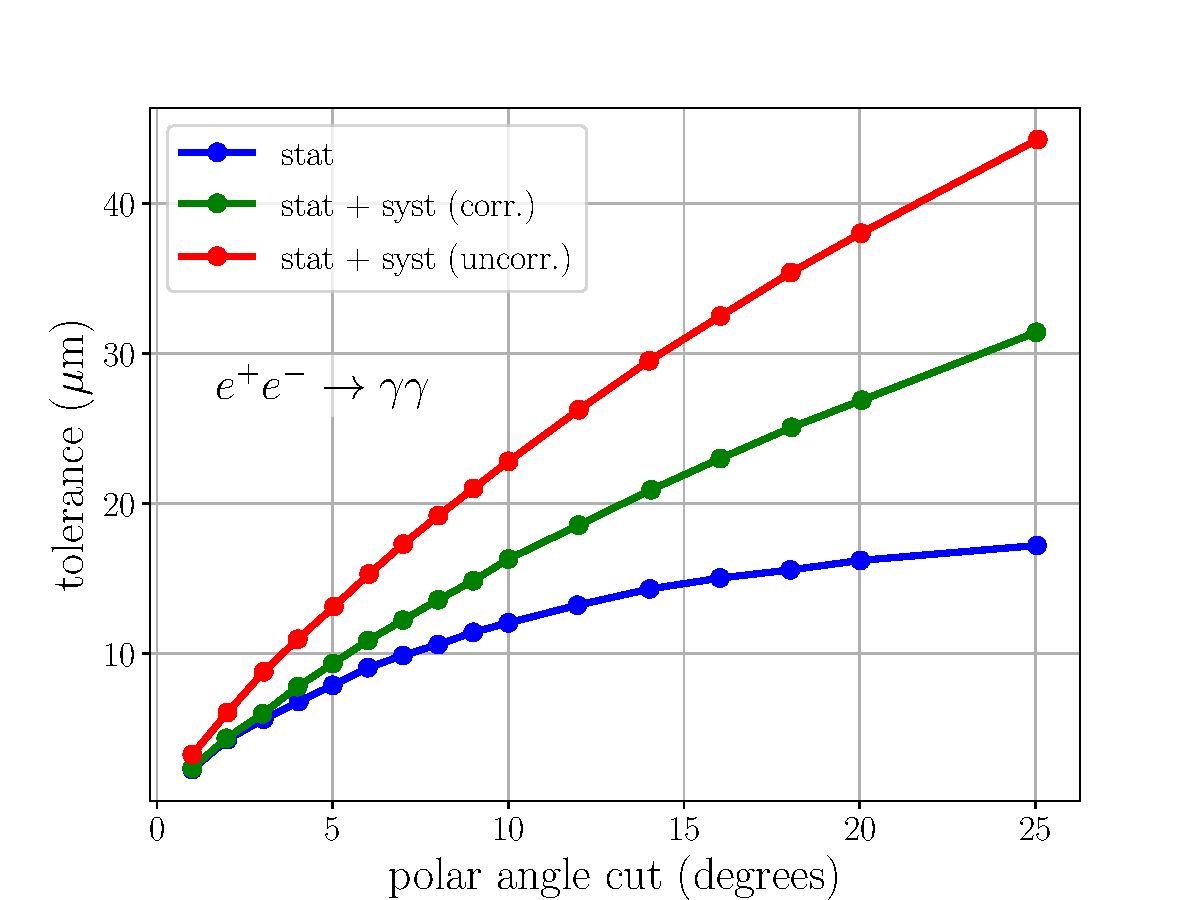
\includegraphics[width=0.48\textwidth]{DetectorRequirements/ECALFIG/DiPhotonTolerance.pdf}
\caption{Tolerance on the accuracy of the polar angle cut as a function of the polar angle cut in degrees, 
expressed as a radial accuracy for a detector situated at 2.5\,m from the IP in the centre-of-mass of the collision. 
Left: For dilepton events, to ensure a systematic precision of $2.2 \times 10^{-6}$. 
Right: For diphoton events, to ensure a systematic precision of $1.5 \times 10^{-5}$ (lower blue curve). 
Also indicated is the tolerance corresponding to having a systematic uncertainty equal to the statistical one, 
assuming either fully correlated (middle green curve) or uncorrelated (upper red curve) displacements in the two endcaps.}
\label{fig:tolerance}
\end{figure}

The definition of the geometrical acceptance (defined, e.g., by a given polar angle lower cut in the centre-of-mass frame of the collision) 
for both $\epem \to \PGg\PGg$ and $\epem \to \ell^+\ell^-$ is an obvious source of a potentially large systematic bias, which was dominant at LEP. 
Indeed, any global or local detector misalignment can generate a systematic bias on the acceptance. 
The tolerance on this bias can be calculated, 
e.g., either to match the resulting systematic uncertainty on the cross section to its statistical precision or to obtain a specific precision, 
as done in Ref.~\cite{Blondel202308} and displayed in Fig.~\ref{fig:tolerance} for a polar angle cut between 1 and 25~degrees.

The tolerance, expressed as the accuracy of the definition of the polar angle cut for a detector situated at 2.5\,m from the IP, is similar for dileptons and diphotons, 
and is in the 10--20\,$\mu$m range for a cut between 10 and 20~degrees, corresponding to a required polar angle accuracy of 4 to 8\,$\mu$rad.

Inspired by the work done for integrated luminosity measurements with low-angle Bhabha scattering at LEP, 
such a tight requirement calls for the design and the construction of the calorimeter (for diphotons) 
and the tracker (for dileptons) endcaps with a mechanical precision ensuring the specified tolerance of 10 to 20\,$\mu$m, 
complemented by dedicated test-beam measurements
and a survey/monitoring of the distance between the two endcaps with a precision of 50 to 100\,$\mu$m. 
While the task is  challenging, it should be kept in mind that for the luminosity monitor (LumiCal), situated at lower angles, 
the transverse (longitudinal) tolerance is of 1\,$\mu$m (50\,$\mu$m) at 1\,m of the luminous region, 
for a precision of $10^{-4}$ on the integrated luminosity measurement~\cite{Dam:2021sdj}. 

With respect to the LEP case, FCC-ee offers an additional totally new and possibly synergistic approach to a precise definition of the acceptance. 
Indeed, the large and constant beam crossing angle of 30\,mrad provides an absolute angular scale to dilepton and diphoton events at all angles. 
Total energy and momentum conservation allows for the event-by-event determination of this crossing angle 
(together with the constant longitudinal boost resulting from the specific positioning of the accelerating RF cavities in the FCC tunnel) 
with excellent accuracy from the final state particle kinematic observables.
A global fit of all events, constraining the crossing angle and the longitudinal boost to be constant, 
would then provide an in-situ local `calibration' of final state particle angles and, in particular, of the acceptance cut. 
The required statistical precision was demonstrated analytically~\cite{JanotFCCWeek} to be within reach with the FCC-ee dilepton and diphoton samples, but the actual fit procedure remains to be 
consolidated\,\footnote{It was already shown in Ref.~\cite{Blondel:2019jmp} that this finite crossing angle and longitudinal boost 
could be used to find and monitor the directions of the $x$, $y$, and $z$ axes within a few $\mu$rad precision every hour at the \PZ pole with dimuon events.}. 
The sensitivity of this approach is proportional to the magnitude of the crossing angle, 
and could not be used with the LEP head-on collisions.
At FCC-ee, it was already shown~\cite{JanotFCCWeek} that a (mechanical or otherwise) tolerance of 100\,$\mu$m in the $r$-$\phi$ direction 
would allow an acceptance definition of 3 to 12\,$\mu$rad, 
irrespective of the (global or local) endcap radial or longitudinal displacements, 
consistent with the tolerances mentioned above, as displayed in Fig.~\ref{fig:PhotonAcc}. 
More recent developments seem to indicate that the required $\phi$ tolerance can also be reached in situ. 

\begin{figure}[ht]
\centering
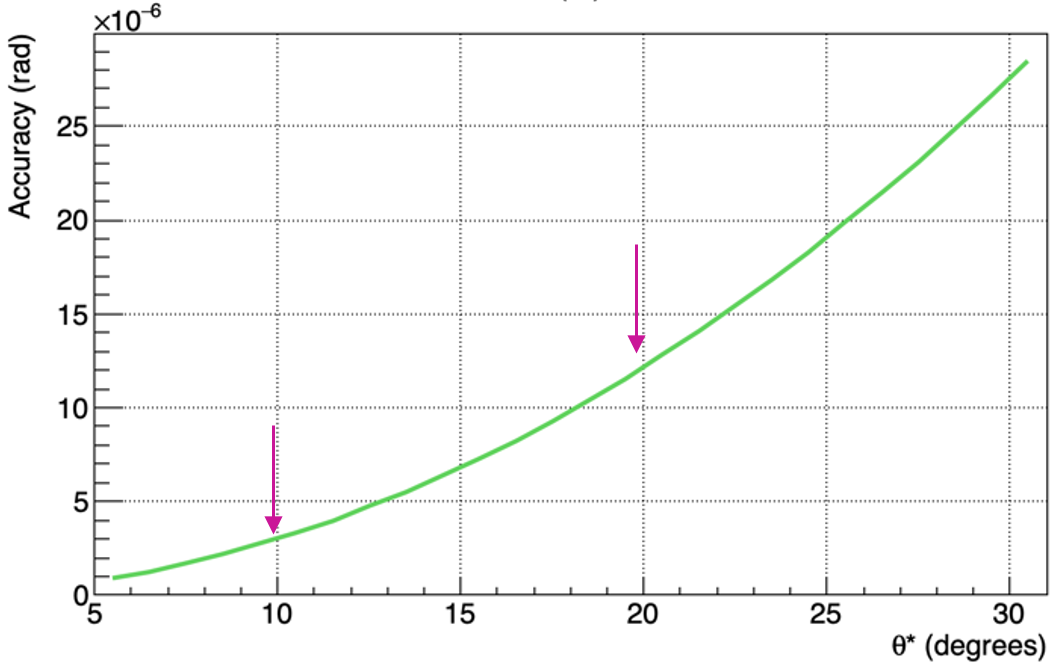
\includegraphics[width=0.6\textwidth]{DetectorRequirements/ECALFIG/DiPhotonAcceptance.png} 
\caption{Analytically-predicted precision of the diphoton acceptance determination (in $\mu$rad) 
as a function of a polar angle cut applied in the event-by-event centre-of-mass frame, 
assuming a 100\,$\mu$m tolerance in the azimuthal direction, 
and exploiting the energy-momentum conservation 
and the constraints that the beam crossing angle and the longitudinal boost are the same (on average) for all events 
and constant in time.
This result is obtained with a readout cell of $1^\circ \times 1^\circ$ and position resolution of $\sigma_{x,y}=0.5$\,mm in the endcap calorimeter 
(commensurate with the various proposed options).}
\label{fig:PhotonAcc}
\end{figure}

Further work is needed to verify the feasibility of the second method beyond analytical computations, 
as well as to evaluate the effect of the beam crossing angle on the acceptance determination with the classical method. 
The large forward cross section of $\epem \to \epem$ events will open the possibility of mutual in-situ alignment of the tracker and the calorimeter, 
offering a cross-check of the acceptance cut. 
It will be important to check whether the second approach would also be suitable for the integrated luminosity measurement 
with low-angle Bhabha scattering in the luminosity monitors. 
The two approaches are expected to help each other, 
either by reducing the mechanical constraints of the former or by improving the convergence of the latter, and most likely both. 
Their combination is expected to provide an excellent understanding of the acceptance, 
a cross-check of their accuracy, and an explicit requirement on the position and angular resolutions of the tracker and of the calorimeter. 

\subsubsection{Sensitivity to charged lepton flavour violation: \texorpdfstring{$\PZ\to \PGm e$}{} and \texorpdfstring{$\PGt\to \PGm\PGg$}{}}

With its $6 \times 10^{12}$ \PZ bosons, FCC-ee enables precise tests of charged lepton flavour violation (cLFV) processes. 
The $\PZ \to \PGm \Pe$  process has an extremely clean signature --- a beam-energy electron recoiling back-to-back against a beam-energy muon --- 
with fully reducible background from the $2 \times 10^{11}$ $\PZ \to \PGt^+\PGt^-$ events. 
It is estimated~\cite{Dam:2021ibi} that FCC-ee will improve by 2 to 3 orders of magnitude 
the current limits of about $10^{-7}$ from the LHC~\cite{Atlas:2022uhq}. 
The most dangerous background comes from the `extreme bremsstrahlung' emission by a muon in a $\PZ \to \PGm\PGm$ event 
that creates a large deposit in the electromagnetic calorimeter, faking an electron. 
This effect could be limited by improving the ECAL energy resolution and having the possibility of longitudinal segmentation to veto showers starting later in the calorimeter. 

The sensitivity of FCC-ee to the LFV $\PGt \to \PGm \PGg$ decay was established in Refs.~\cite{Dam:2021ibi, Dam:2018rfz}
and the major detector effects on the measurement were evaluated. 
The analysis strategy requires the identification of a clear SM \PGt decay on one side (`tag') 
so that the search for the LFV decay is performed in the other hemisphere. 
The discriminant variables are the total energy and the invariant mass of the final state. 
As shown in Fig.~\ref{fig:taumugamma}~(left), the signal region is background dominated and 
the background density rises linearly away from the $E_{\PGm\PGg} - E_\text{beam}=0$ line. 
This implies that the sensitivity (upper limit) scales linearly with the $E_{\PGm\PGg}$ resolution, which is dominated by the ECAL energy resolution. 
With the full event sample of $4 \times 10^{11}$ \PGt decays, 
an expected 90\%~CL upper limit of $1.2\times 10^{-9}$ can be reached~\cite{Lusiani:2024tau}, 
as shown in Fig.~\ref{fig:taumugamma}~(right).

\begin{figure}[ht]
\centering
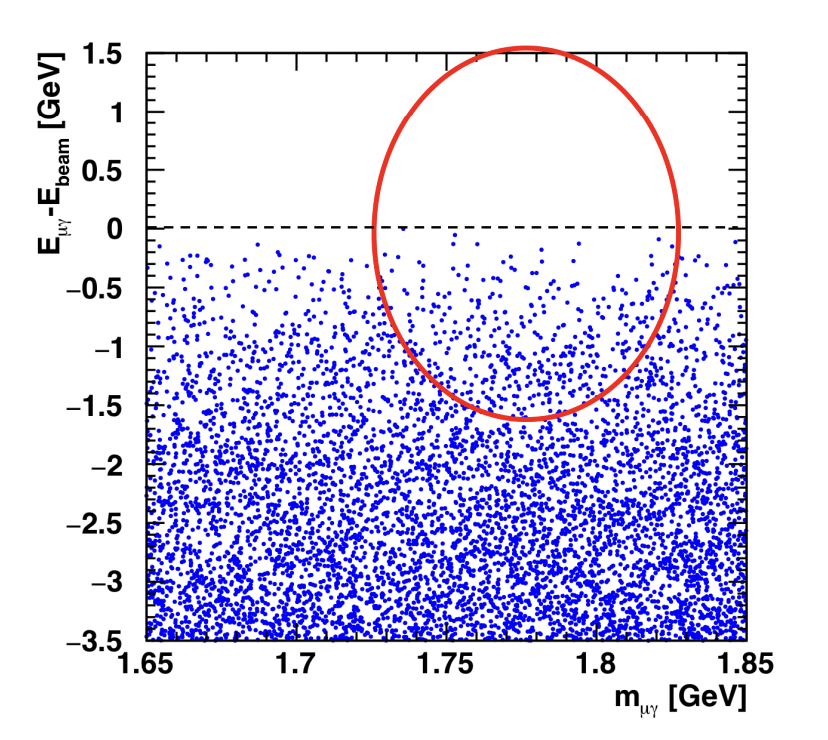
\includegraphics[width=0.4\textwidth]{DetectorRequirements/ECALFIG/taumugamma.png}
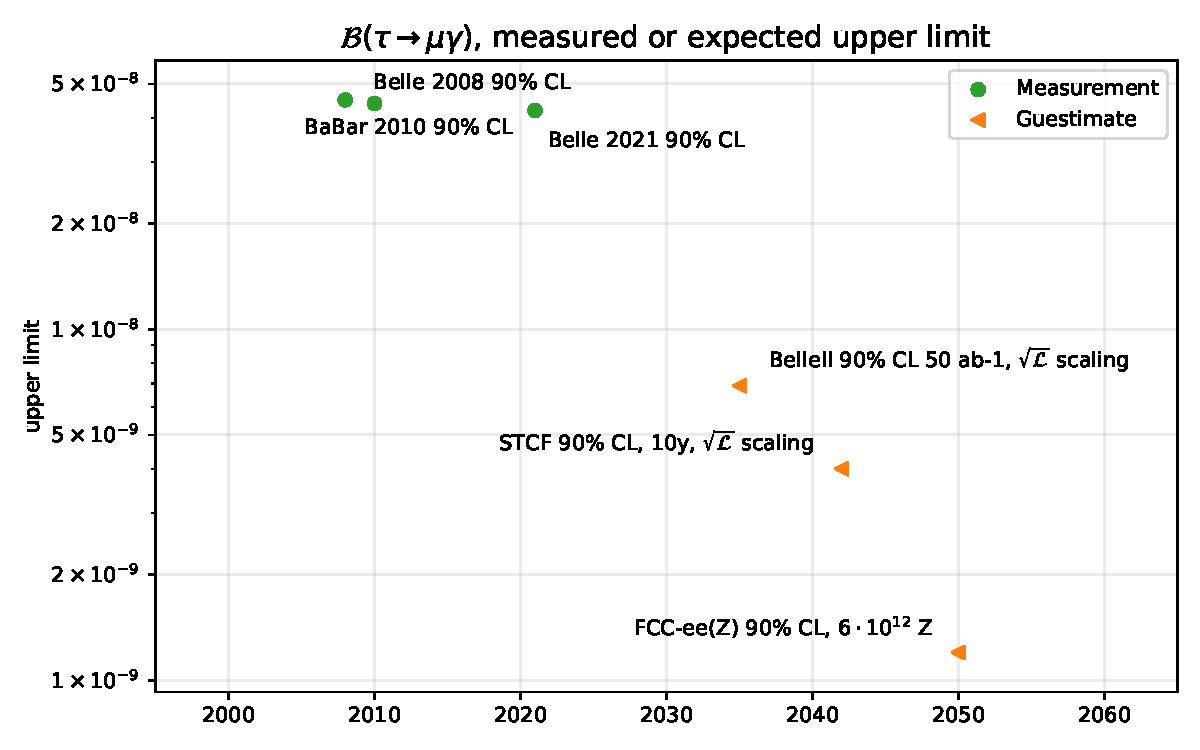
\includegraphics[width=0.58\textwidth]{DetectorRequirements/ECALFIG/exp-ul-90cl-tau-mu-gamma-1.pdf}
\caption{Left: Reconstructed energy vs.\ mass for all $\PGm\PGg$ combinations in simulated $\PZ \to \PGt\PGt\PGg$ background events with one $\PGt \to \PGm \PAGn \PGn$ decay. 
The signal region corresponding to 2\,$\sigma$ resolution is indicated by the red ellipse. 
Right: Present and expected upper limits for ${\cal B}(\PGt\to\PGm\PGg)$~\cite{Lusiani:2024tau}. 
The dates of the future measurements are mainly chosen for plotting purposes. 
The expected limits for Belle~II and the Super Charm-Tau factories are conservative estimates, assuming that those searches will be mostly background-constrained.}
\label{fig:taumugamma}
\end{figure}

This benchmark is particularly interesting because it also shows a requirement for the photon position resolution, which contributes to the invariant mass calculation.  
In this example, where the calorimeter has a resolution of about $16.5\%/\sqrt{E}$ (as in CLD) and a position resolution of 2\,mm, 
the two contributions in the invariant mass calculation are similar. 
Therefore, for this measurement, while the sensitivity is found to scale linearly (or slightly more strongly) with the photon energy resolution, 
a fine-grained crystal calorimeter with a $3\%/\sqrt{E}$ energy resolution would be particularly valuable. 
This is especially true since it would also provide a significantly better spatial resolution, of around 1\,mm, 
leading to a fivefold improvement in sensitivity compared to the previous example.

\subsubsection{Bremsstrahlung recovery}

Even with an excellent EM calorimeter resolution, 
for 50\,GeV central electrons the resolution of a calorimetric measurement is worse than the resolution of the tracker determination of the momentum. 
Furthermore, the latter is not as good as that of muons since electrons emit bremsstrahlung radiation: 
even with the light tracker of IDEA, corresponding to $\sim$\,10\% of a radiation length in the central region, 
the effective momentum resolution of electron tracks is at least a factor of two worse than that of muons~\cite{note_bremRecovery}. 
Several measurements call for a better electron momentum resolution. 
For example, the determination of the Higgs boson mass from $\PZ(\PGm\PGm)\PH$ events (Section~\ref{sec:PhysPerf_HiggsRecoil}) 
can gain from exploiting the $\PZ \to \epem$ channel. 
A resolution improvement can be brought by the recovery of the bremsstrahlung photons in the calorimeter, 
if their energy can be added to the momentum of the track. 
An effective recovery requires that the showers of the electron and of the radiated photon(s) be disentangled by the reconstruction algorithm. 
For 50\,GeV central electrons, in a 2\,T magnetic field, photons radiated at small radii 
(where, in the IDEA tracker, most of the bremsstrahlung emissions happen) 
are separated by typically 2--3\,cm from the electron at the calorimeter entrance.  
The ability to separate showers that are so close to each other calls for a transverse granularity of $1 \times 1$\,cm$^2$ or better 
and may place some demands on the longitudinal segmentation, which helps to disentangle showers that partially overlap. 
Detailed \textsc{Geant} simulations and reconstruction algorithms are needed for a precise assessment of these constraints. 
Meanwhile, it is estimated that, with the recovery of bremsstrahlung photons, 
the effective resolution of electrons would be 25\% (45\%) worse than the muon resolution 
for a calorimeter EM energy resolution of $3\% / \sqrt{E}$ ($15 \% / \sqrt{E}$). 
More details can be found in Ref.~\cite{note_bremRecovery}. 
The \textsc{Delphes} simulations used for the studies reported in this document rely on this estimation. 
With this bremsstrahlung recovery, the $\PZ \to \epem$ channel significantly contributes to the determination of the Higgs boson mass from $\PZ\PH$ events, 
as shown in Fig.~\ref{fig:mH_recoil-ee}, improving the uncertainty by 22\% compared to what is obtained from the muon channel alone~\cite{HiggsNoteRecoil}.

\begin{figure}[ht]
\centering
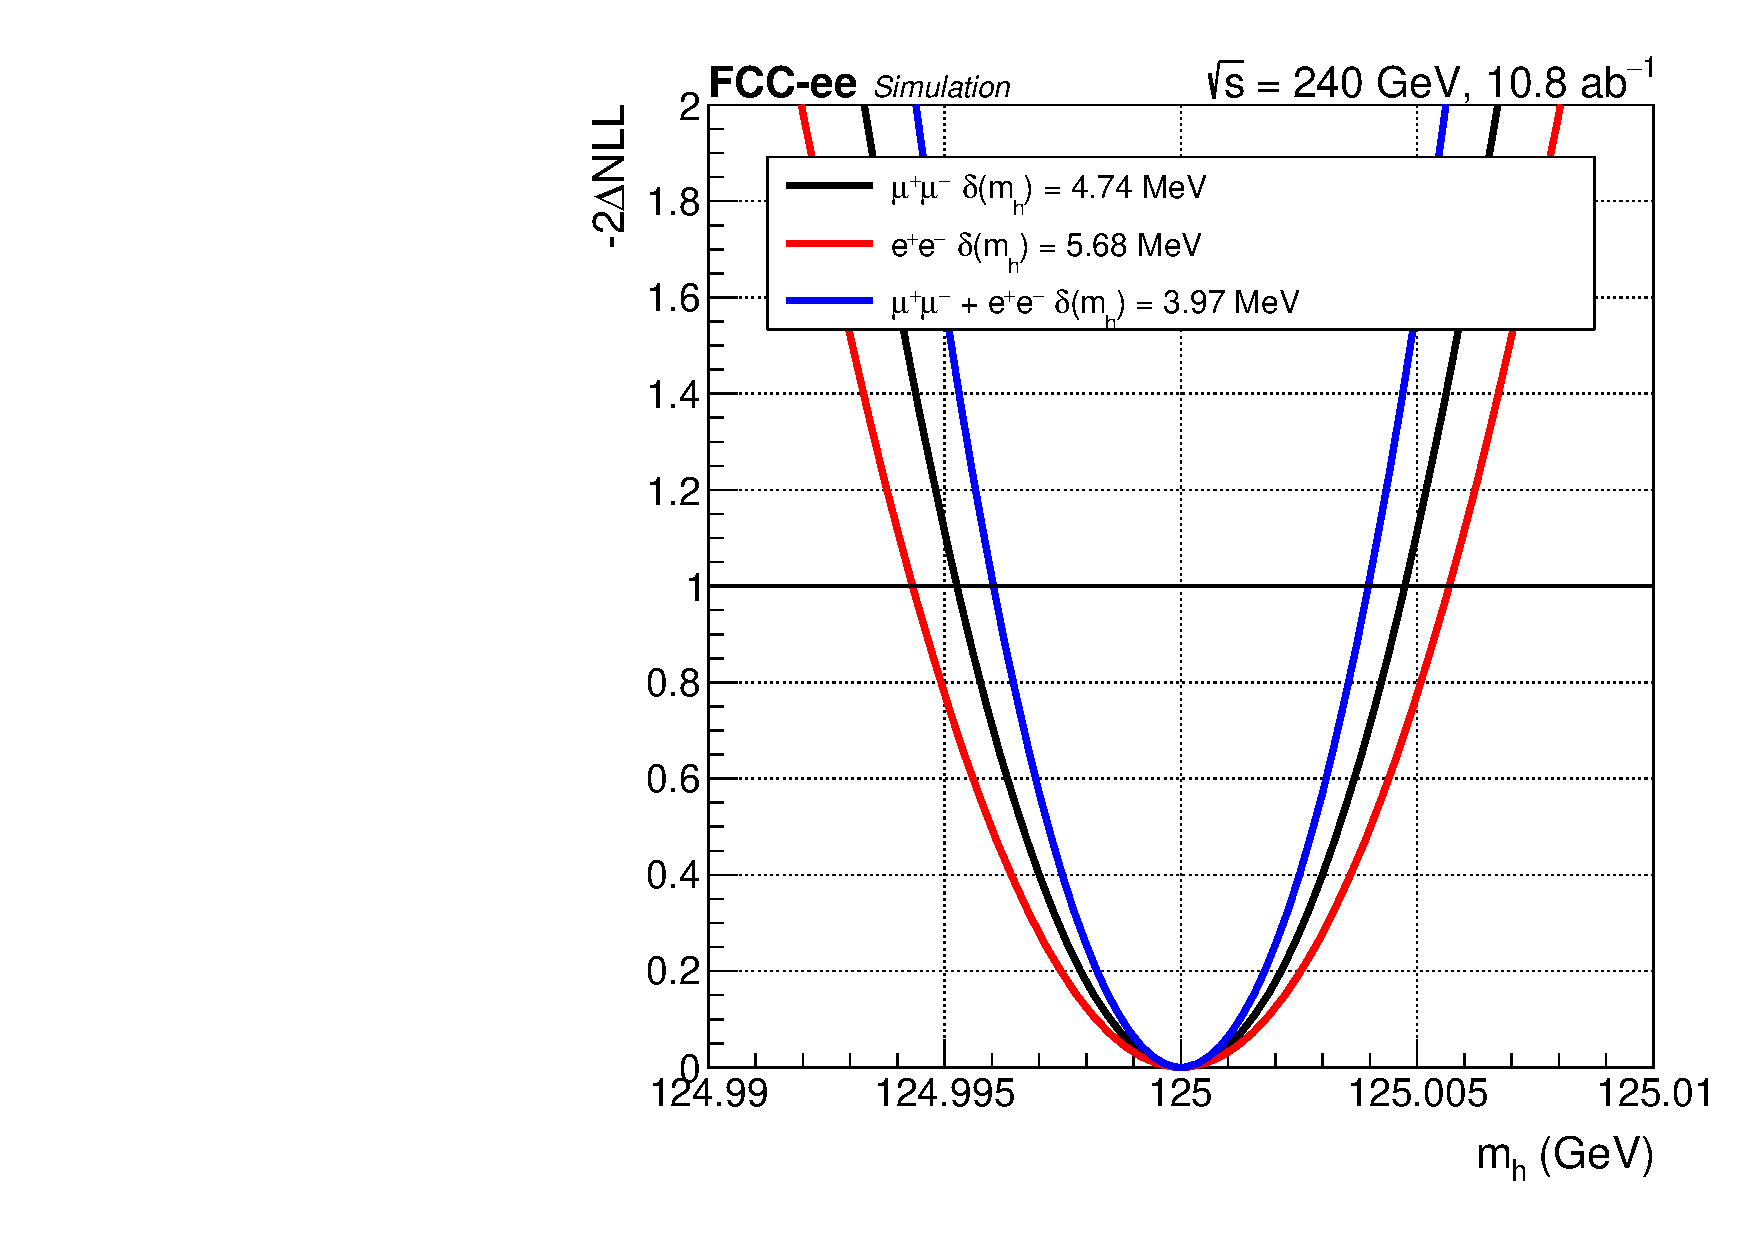
\includegraphics[width=0.45\textwidth]{DetectorRequirements/Figs/HiggsRecoil_mumu_ee_categorized.pdf} 
\caption{Likelihood scan of the Higgs boson mass with the recoil method, combining the muon and electron channels. 
The uncertainties correspond to the quadratic sum of the statistical and systematic terms.}
\label{fig:mH_recoil-ee}
\end{figure}

\subsubsection{Prompt decays of ALPs \texorpdfstring{$\axion \to \PGg \PGg$}{a to gamma gamma}}

A search for ALPs produced in $\PZ \to \axion \PGg$ decays, complementary to the one previously mentioned, 
consists in looking for ALPs that decay promptly into two photons, leading to a three-photons final state. 
The analysis presented in Ref.~\cite{note_ALP_Polesello} compares the sensitivities that are expected with the dual-readout fibre calorimeter of IDEA 
and with the variant where crystals are placed in front of it.

The experimental sensitivity is driven by the ability to precisely reconstruct the invariant mass of the two photons coming from the ALP decay. 
For low masses, up to a few hundreds of MeV, the resolution on this diphoton mass is dominated by the resolution on the photon angles, 
hence by the precision with which the impact point of the photons at the calorimeter entrance is determined. 
This contribution decreases with increasing ALP mass and, above 10\,GeV, the resolution depends only on the energy resolution of the calorimeter. 
In addition, at low masses, below $\sim$\,5\,GeV, the two photons from the ALP decay may not be resolved in the detector but be `merged' into a single reconstructed object.
Detailed \textsc{Geant} simulations and reconstruction algorithms, still under development, are needed for a precise understanding of these effects. 
A simplified approach is adopted for the current sensitivity study, 
whereby the angular distance $\Delta \alpha$ between the two photons is used to determine whether the photons are resolved.
Taking into account the transverse granularity and the Moli{\`e}re radius of the detectors, 
it is assumed that photons with $\Delta \alpha > 20$\,mrad can be reconstructed in the crystal calorimeter, 
which corresponds to a separation of 4\,cm (four calorimeter cells) of the two photons at the calorimeter entrance. 
For the dual-readout calorimeter, photons are required to be separated by $\Delta \alpha > 10$\,mrad to be resolved, 
which corresponds to the distance between 10 fibres of the detector.

Taking into account the irreducible $\epem \to \PGg\PGg\PGg$ background, 
the experimental reach expected for the two calorimeter options is shown in Fig.~\ref{fig:ALPs_prompt}. 
The crystal calorimeter has a better sensitivity for high masses, where the sensitivity is driven by the energy resolution.
The impact point resolution is very similar for the two calorimeters, 
but the better granularity of the fibre calorimeter is expected to provide a better separation for collimated photons that emerge from the decay of ALPs at very low masses, 
resulting in a gain in sensitivity compared to that provided by the crystal detector.

\begin{figure}[ht]
\centering
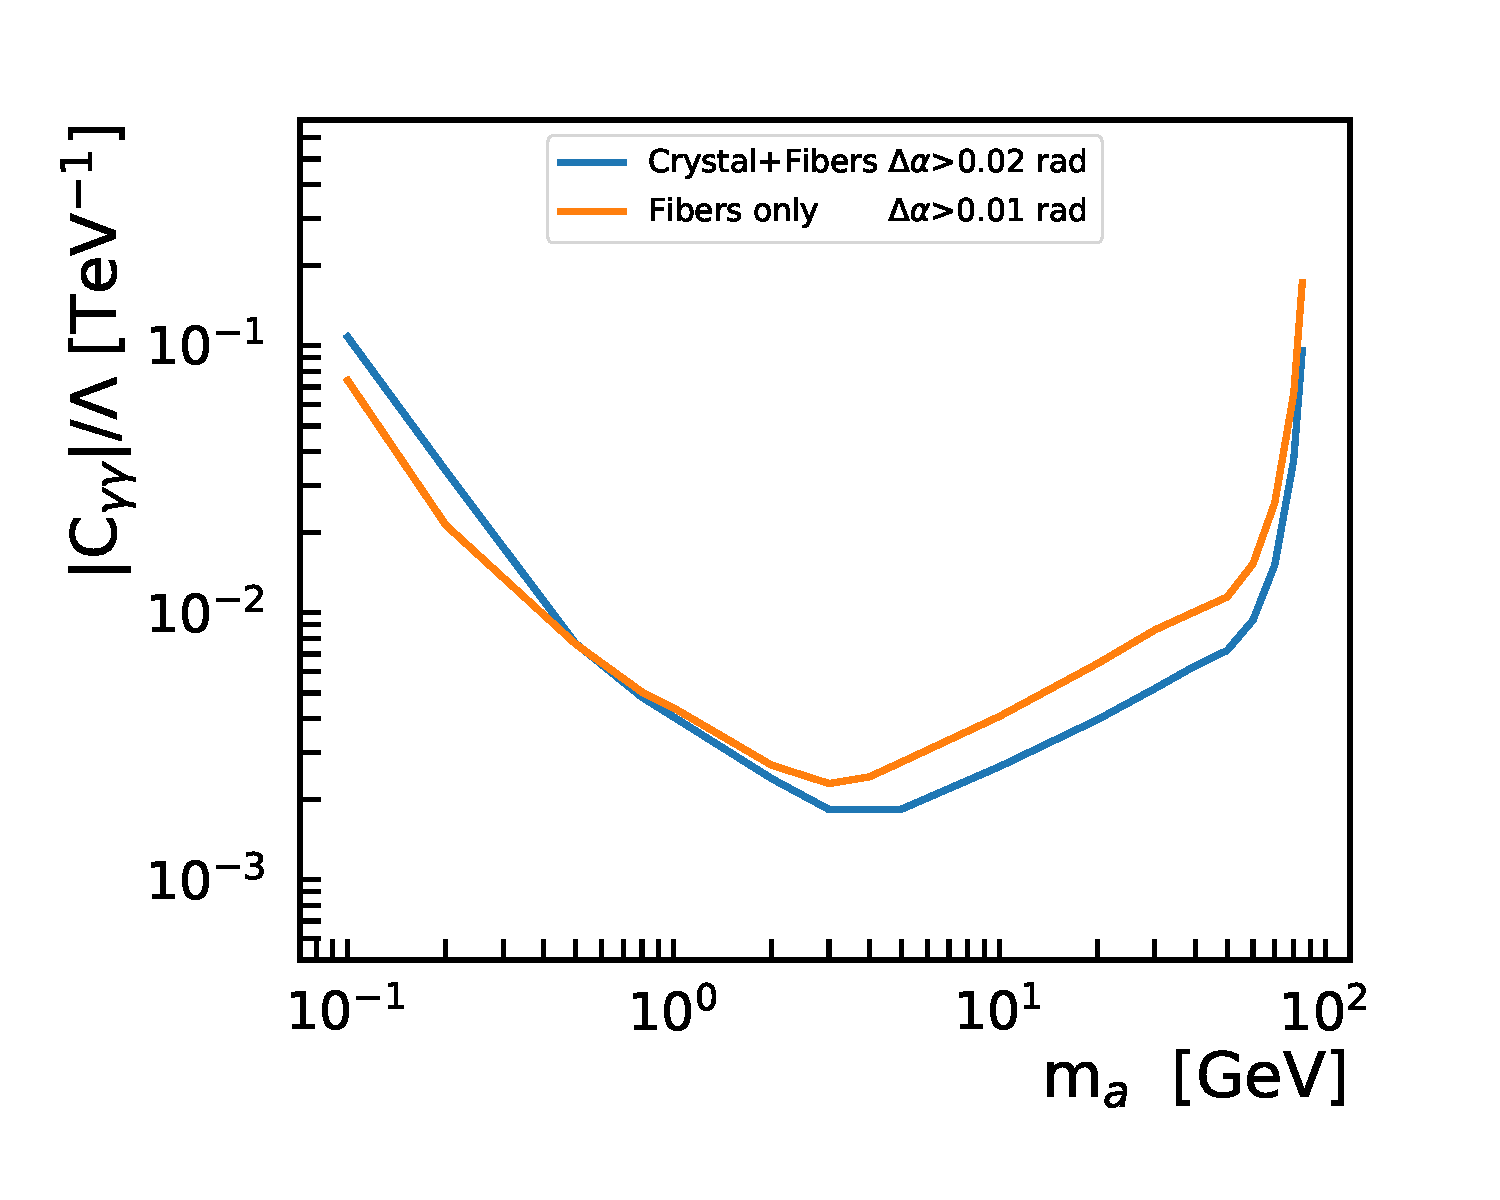
\includegraphics[width=0.5\textwidth]{Physics/DetectorRequirements/Figs/ALPs_prompt2calo.pdf} 
\caption{Expected sensitivity at the 2\,$\sigma$ level of a FCC-ee experiment, 
in the parameter space spanned by the mass of the ALP and its coupling to two photons, 
from a search for ALPs that decay promptly into two photons. 
In the legends, $\Delta \alpha$ denotes (in rad units) the angular separation down to which the calorimeter is assumed to be able to resolve two photons.}
\label{fig:ALPs_prompt}
\end{figure}

As shown by Fig.~\ref{fig:ALPs_prompt}, the parameter space covered by this analysis, that focuses on prompt decays of ALPs, 
nicely complements the one explored by a search or quasi-stable ALPs in the monophoton final state (Fig.~\ref{fig:PhysPerf_ALPs_monophotons}). 
The sensitivity to ALPs with intermediate lifetimes, which are long-lived but decay inside the detector, is more difficult to assess. 
For ALPs that decay before reaching the calorimeter, it depends on the ability to reconstruct the displaced decay vertex of the ALP into two photons. 
For ALPs that decay inside the calorimeter, the sensitivity depends on the ability to identify late-starting showers. 
The requirements that these analyses will place on the longitudinal segmentation of the calorimeter, on the measurement of the timing of calorimeter signals, 
and on a potential preshower, remain to be studied.

\subsubsection{Requirements from \texorpdfstring{$\PGpz \to \PGg\PGg$}{pi0 to gamma gamma} reconstruction in \texorpdfstring{\PGt}{tau} decays}
\label{sec:PhysPerf_Pi0sFromTaus}

The reconstruction of $\PGpz \to \PGg\PGg$ decays is a crucial component for several measurements of the FCC-ee physics programme, 
such as the tau branching ratios or the tau polarisation. 
The kinematic of a $\PGt \to \PGr\PGn$ decay produced at the \PZ pole provides initial detector requirements~\cite{KWandallThesis}. 
For instance, the momentum of the \PGpz produced in the \PGr decay is quite soft and its decay photons are even softer.
The capability of identifying these low-energy photons requires a low noise and high energy resolution calorimeter. 
The energy resolution is important also because it affects the \PGpz identification itself, which relies on a cut on the diphoton invariant mass.
The granularity is another important aspect that plays a role in the separation of the two photons. 
The angular separation between the two photons, $\approx 2 m_{\PGpz} / E$, is typically 10\,mrad, 
which leads to a separation of 2\,cm at the calorimeter entrance; 
however, for the highest possible energy ($E_{\PGpz} = 45.6$\,GeV) the opening angle is reduced to 6\,mrad, 
corresponding to 1.2\,cm separation at the calorimeter 
entrance\footnote{A large tracking volume, optimised for track momentum resolution, 
is also beneficial for the identification of collimated objects such as \PGpz decays.}. 
The granularity is also needed for the correct separation of the photons from charged pions in the decays. 
A study has been done comparing the performance of different noble liquid calorimeters (LAr and LKr) in \PGpz events. 
Cases have been considered where the photons from the \PGpz decays can be reconstructed separately (resolved) 
or are reconstructed as a single EM object (unresolved).
As seen in Fig.~\ref{fig:Pi0RecoComp},
the \PGpz reconstruction efficiency and the \PGpz mass resolution are better in the LAr option with the finer granularity 
and improve further in the LKr option, given its smaller Moli\`ere radius.

\begin{figure}[ht]
\centering
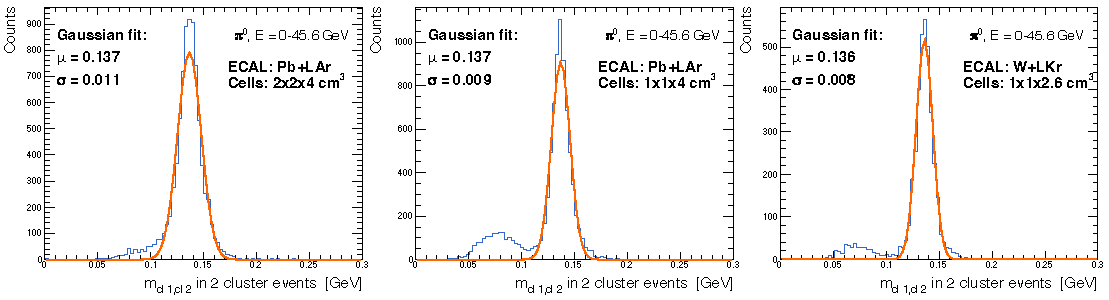
\includegraphics[width=\textwidth]{DetectorRequirements/Figs/Two-cluster-pi0-massDistr.pdf} 
\caption{Invariant mass distributions of two-cluster \PGpz mesons for different noble liquid calorimeter configurations.} 
\label{fig:Pi0RecoComp}
\centering
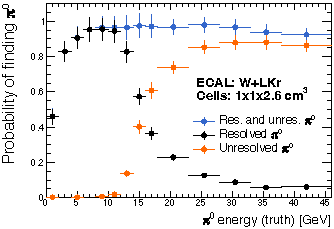
\includegraphics[width=0.5\textwidth]{DetectorRequirements/Figs/pi0-id-prob-vs-pi0-energy-LKr.pdf} 
\caption{Probability of \PGpz identification as a function of its energy for a W$+$LKr calorimeter with a granularity of $1\times 1\times 2.6$\,cm$^3$.}
\label{fig:Pi0Reco}
\end{figure}

Figure~\ref{fig:Pi0Reco} shows the \PGpz reconstruction efficiency, as a function of its energy, all the way to 45\,GeV. 
Above 40\,GeV, the transverse shape of an unresolved \PGpz electromagnetic shower resembles more and more that of a single photon 
and the identification efficiency progressively vanishes.

\subsubsection{Work ahead}
\begin{itemize}

\item The measurement of tau polarisation in \PZ decays, from which the tau and electron asymmetries, $A_{\PGt}$ and $A_{\Pe}$, are extracted, 
is a cornerstone of the Tera-\PZ physics programme. 
Experience from LEP shows that the precision of this measurement critically depends, in particular, on the design of the electromagnetic calorimeter. 
While the sizes of the event samples used by the four LEP experiments were similar, 
the uncertainties differed by nearly a factor of two from one experiment to the other. 
As noted above, a high calorimeter transverse granularity is indeed crucial to identify and precisely reconstruct the \PGpz mesons produced in \PGt decays. 
The precision that different detector concepts can achieve on this measurement needs to be studied with a full simulation description, 
which also includes, besides the spatial and energy detector resolution, the effect of fake photons. 
Work in this direction has started, as is shown in Section~\ref{sec:PhysPerf_FullSim}.

\item The reconstruction of the events on fully simulated detector concepts will be crucial to extract further requirements on the detector performance. 
For instance, since photon energy contributes 25\% of the total energy of a jet, 
the ability to reconstruct low-energy photons is very important in order to improve the jet energy resolution, 
which is crucial for Higgs boson hadronic final states, such as $\PH \to \Pg\Pg$. 
Moreover, in a study considering multi-jet topologies~\cite{Lucchini:2020bac} it has been shown 
that the absence of photon and \PGpz identification prior to the jet particle-flow reconstruction 
would worsen the resolution of the reconstructed hadronic objects in about one third of the cases. 
Preliminary studies will need to be updated once the reconstruction of full simulation detector concepts become available in the coming months. 

\item The measurement of long-lived particles decaying to photons relies on a precise standalone ECAL measurement of the direction of the shower. 
The impact of longitudinal segmentation on the pointing capabilities and on displaced vertex reconstruction performance needs to be studied in full simulation.

\end{itemize}

\subsubsection{Preliminary conclusions}

\begin{itemize}

\item An electromagnetic calorimeter with excellent energy resolution (a few \%) is required to optimise the expected precision on the \PZ to \PGne coupling 
via the $\epem \to \PGne \PAGne \PGg$ process, 
lepton flavour violating decays such as $\PZ  \to \PGm \Pe$ and $\PGt \to \Pe \PGg$, 
decays of heavy flavoured hadrons to photons or \PGpz, 
and ALPs searches. 

\item Excellent transverse granularity and resolution is needed for optimal Bremsstrahlung recovery and \PGpz identification. 
Longitudinal segmentation and pointing capabilities are required for displaced photon vertex identification, such as long-lived ALP decays. 

\item A knowledge of the acceptance at the level required to match the statistical precision on the $\epem \to \PGg \PGg$ cross section 
for the absolute luminosity determination requires that the calorimeter be constructed with a mechanical precision of few tens of microns. 

\item Reconstructing low energy photons from decays of \PGpz mesons, either produced in \PB or \PD decays or in $\PH \to \Pg\Pg$,
requires as little material in front the ECAL as possible, as well as a noise term as small as a few tens of MeV. 

\end{itemize}

\subsection{Requirements for the hadron calorimeter}
\label{sec:PhysPerf_HadCal}

To fully exploit the statistical power of FCC-ee, precise measurements of processes in their hadronic final states are crucial because of their typically large branching ratios. 
A clear advantage of $\epem$ collisions over hadron collisions, such as at the HL-LHC, 
is the almost negligible pile-up and the absence of underlying event and initial-state QCD radiation, 
as well as the precise knowledge of the total energy-momentum of the final state,
resulting in cleaner data and improved jet energy resolutions.
For FCC-ee, the possibility of having a full \textsc{Geant} simulation of the events in the new software has become available only recently, 
so that a state-of-the-art event reconstruction based on the particle flow approach is not yet validated for complete physics studies.  
Since the reconstruction algorithm significantly impacts the final resolution on hadronic objects, 
it is challenging to determine specific requirements for the hadron calorimeter performance from existing studies, performed with fast simulation \textsc{Delphes} samples. 
Nevertheless, valuable information can be derived regarding the overall impact that the performance of the calorimeter has on the accuracy of the measurement, 
profiting from the particle-flow inspired reconstruction available in \textsc{Delphes}.

\subsubsection{Reconstruction of Higgs boson hadronic final states}

The identification of $\PH \to jj$ signal events relies on the resolution of the dijet system mass, which is influenced by the performance of the calorimeter. 
Additionally, the precise separation of different flavours depends on the effectiveness of the flavour tagging algorithm, 
which also imposes requirements on the vertex detector and on particle identification, as discussed in Sections~\ref{sec:PhysPerf_Hcc} and~\ref{sec:PhysPerf_strangeTagging}. 
Assuming an ideal particle-flow algorithm, with perfect charged and neutral particle identification, 
the visible energy (and mass) resolution is dominated by the neutral hadron resolution, 
which is in turn driven by the HCAL stochastic term. 
A study has been performed to assess the impact of a degraded hadron calorimeter performance~\cite{sciandra_2024_gt813-z8602}, 
by worsening the HCAL stochastic term (50\% and 100\%) and then compare the resulting $\PH \to jj$ sensitivity to that of the IDEA detector baseline 
(which assumes dual-readout calorimetry with a 30\% stochastic term).

\begin{figure}[ht]
\centering
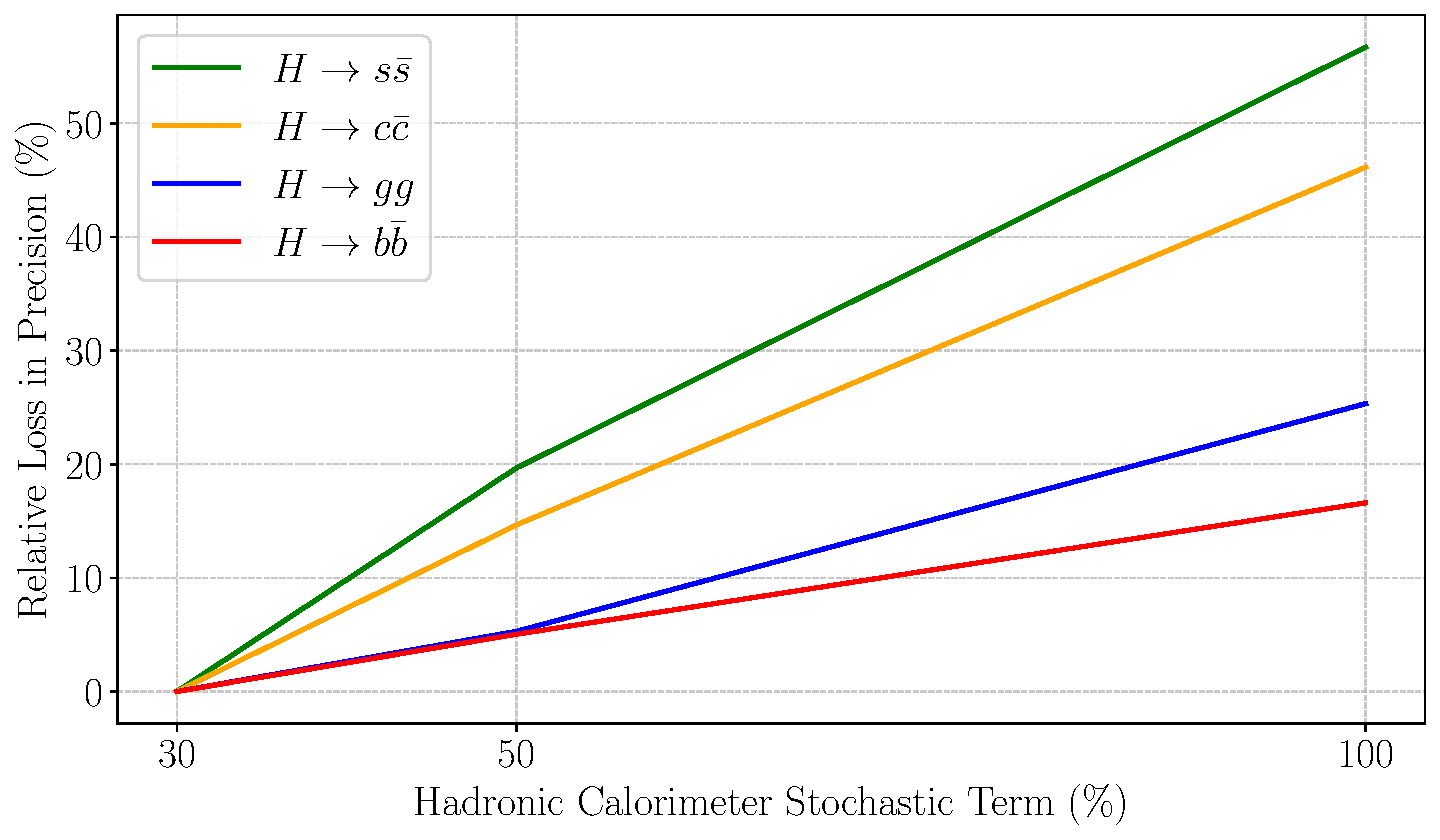
\includegraphics[width=0.7\textwidth]{Physics/DetectorRequirements/Figs/relative_loss_vs_stochastic_term.pdf} 
\caption{Expected precision degradation of the branching ratio measurements for the $\PH \to \PQb\PAQb$, $\PQc\PAQc$, $\PQs\PAQs$, and $\Pg\Pg$ decays 
as a function of the HCAL stochastic term. 
To guide the interpretation, the value 30\% would correspond to a dual-readout calorimeter as in the baseline IDEA simulation, 
50\% corresponds to an ATLAS-type calorimeter, and 100\% to a CMS-type calorimeter.}
\label{fig:HiggsBRPrec_vs_HadRes}
\end{figure}

The results are summarised in Fig.~\ref{fig:HiggsBRPrec_vs_HadRes} for several Higgs boson decay channels. 
When the neutral hadron energy stochastic term is degraded to 50\% (100\%), the expected precision of the measurement of the $\PH \to \PQs\PAQs$ branching ratio degrades by about 20\% (55\%).
The larger is the expected signal-to-background ratio in a given channel (the largest being for $\PH \to \PQb\PAQb$), 
the smaller is the effect of the degradation of the neutral hadron energy resolution on the expected precision. 
The visible mass resolution is, therefore, particularly important for accurately measuring the $\PH \to \PQc\PAQc$ and $\PH \to \PQs\PAQs$ branching fractions.

\subsubsection{Measurement of the Higgs boson invisible width}

As discussed in Section~\ref{sec:PhysPerf_HiggsRecoil}, FCC-ee offers a unique opportunity to use the `recoil method' for precise, model-independent measurements of Higgs boson properties. 
This method becomes particularly valuable when studying the Higgs boson decay into an invisible final state. 
The Standard Model process $\PH \to \PGn\PAGn\PGn\PAGn$ has a very small branching ratio, $1.06\times 10^{-3}$~\cite{deFlorian:2227475}, 
so that it is beyond the reach of the LHC programme and might only be observable at the FCC-hh. 
However, with possible extensions of the Standard Model, such as the inclusion of a Higgs portal, 
the Higgs boson width to invisible final states could be increased because of decays to non-SM particles, 
which could be potential dark matter candidates~\cite{Patt:2006fw, sym13122406}, making the study of this channel highly relevant.

In a recent study~\cite{HiggsInvisibleNote}, the \textsc{Delphes} simulation of the IDEA detector was used, 
along with the state-of-the-art flavour tagging algorithm \textsc{ParticleNetIDEA}, described above. 
To maximise the size of the event sample, the analysis considers not only \PZ decays to $\Pe\Pe$ and $\PGm\PGm$ but also to $\PQb\PAQb$, $\PQc\PAQc$, and $\PQq\PAQq$. 
The visible mass ($M_\text{vis}$) serves as the discriminant variable in the final fit (with no systematic uncertainties considered at this stage). 
The results indicate that, with an integrated luminosity of 10.8\,ab$^{-1}$ at $\sqrt{s} = 240$\,GeV and of 3\,ab$^{-1}$ at $\sqrt{s} = 365$\,GeV, a measurement of the SM branching ratio with a precision of 25\% could be achieved. 
Furthermore, when accounting for the possibility of exotic decays, the study results in the exclusion, at the 95\% CL, of branching fractions lower than 0.05\%, or a 5\,$\sigma$ observation if greater than 0.13\%. 
The $\PZ \to \PQq\PAQq$ decay channel was found to be the one with the best sensitivity, given its higher statistical power, and the run at $\sqrt{s} = 240$\,GeV has much better sensitivity than the highest energy run.
A preliminary study performed with CLD full simulation can also be found in Ref.\cite{sciandra_2024_gt813-z8602}.

\begin{figure}[ht]
\centering
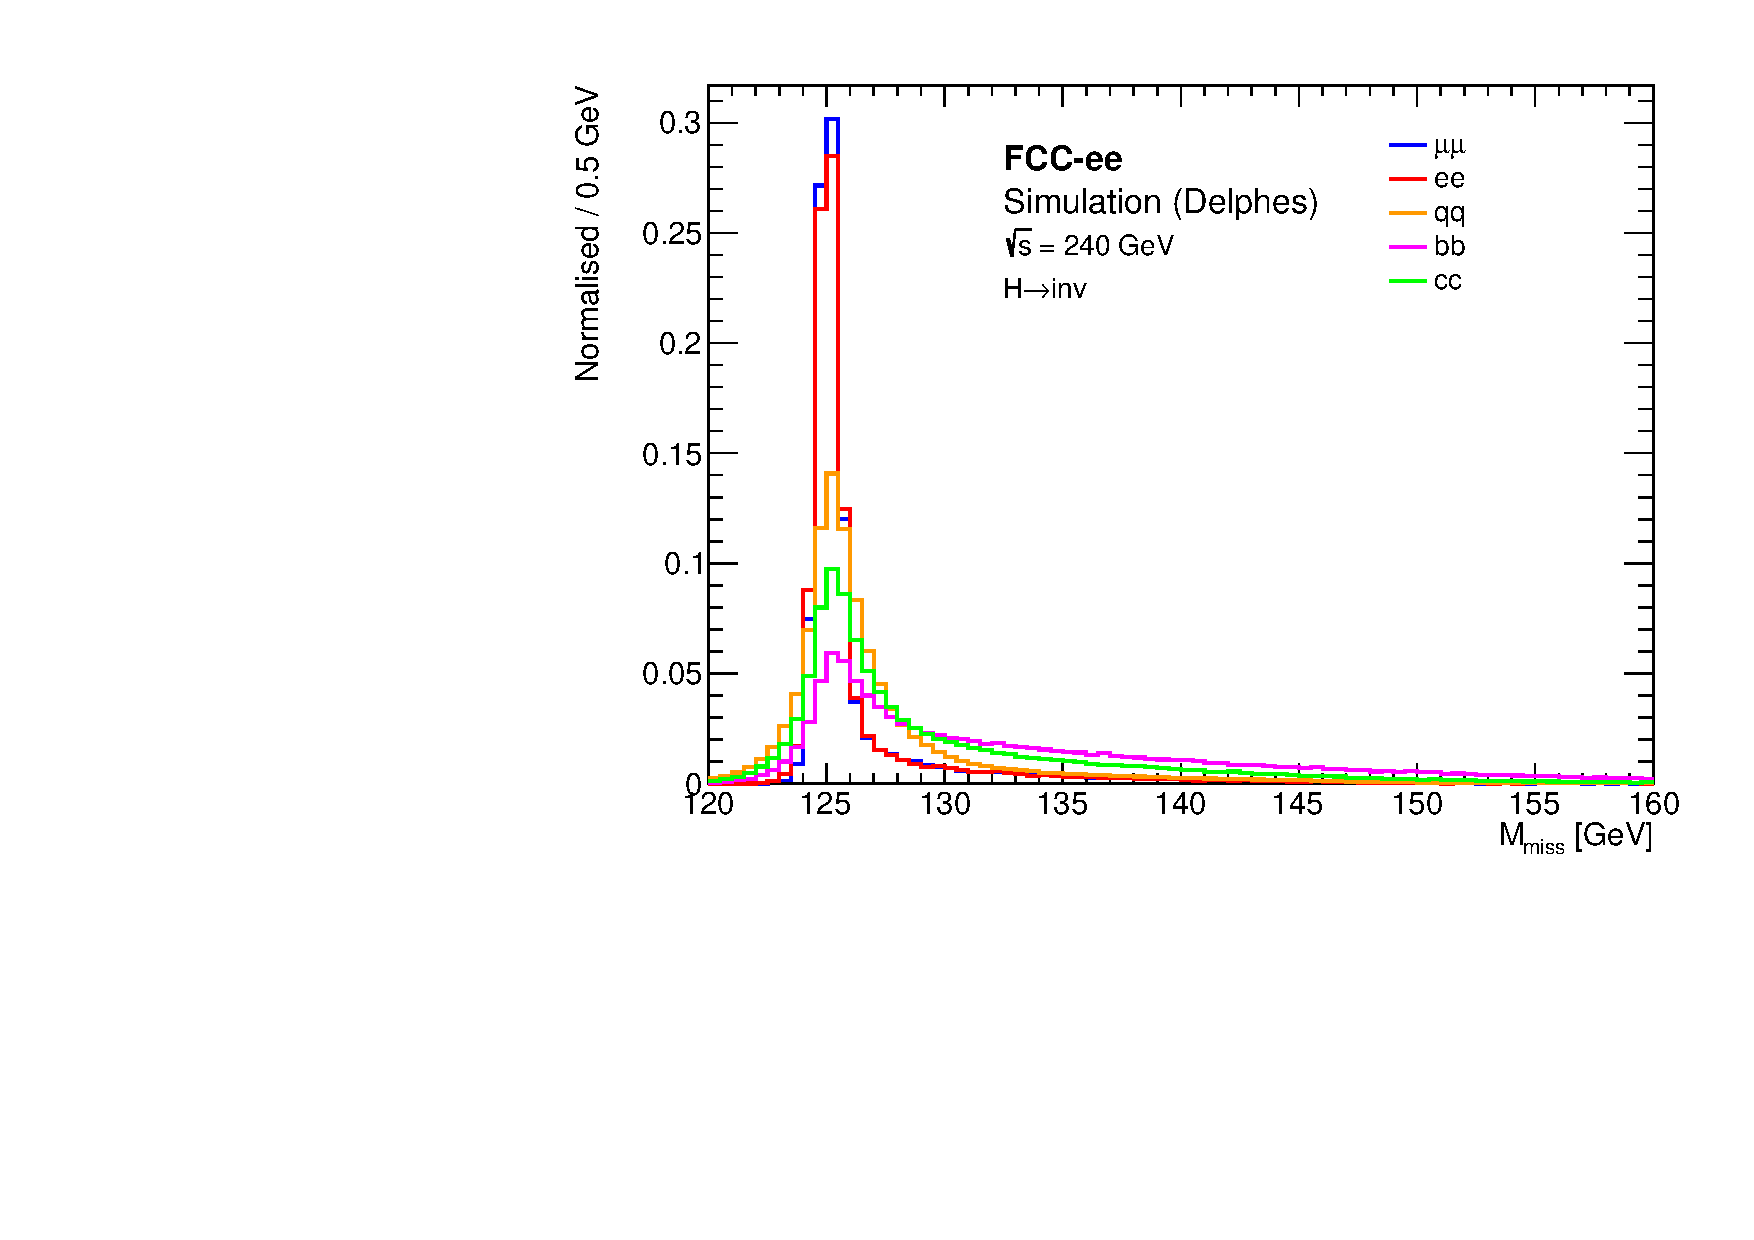
\includegraphics[width=0.7\textwidth]{Physics/DetectorRequirements/Figs/Hinv_SignalDistribution_0.5_ver2.pdf} 
\caption{The $M_\text{miss}$ distribution for several \PZ decay channels, corresponding to the Higgs boson signal, in $\PH\PZ$ processes. 
The distributions are normalised to the same number of events and are shown after the $P_\text{miss}>10$\,GeV cut and the $M_\text{vis}$ selection around the \PZ mass.}
\label{fig:Hinv_Mmiss}
\end{figure}

Figure~\ref{fig:Hinv_Mmiss} displays the normalised distribution of the missing mass, representing the Higgs boson, 
for the various \PZ decay modes, allowing the comparison of resolutions between the lepton and hadron channels. 
An investigation was also conducted into the effects of a poorer detector energy resolution on the measurement, 
applying a simple additional Gaussian smearing to the four-vector of the hadronic final state. 
As shown in Fig.~\ref{fig:Hinv_resStudy}, an additional smearing of 5\% led to a 130\% (80\%) increase in the uncertainty on the $\PQq\PAQq$ channel (combined result).
The blue dashed curve in Fig.~\ref{fig:Hinv_resStudy} represents the resolution of the reconstructed Higgs boson mass for the case where the \PZ boson decays into hadronic modes, as a function of the additional smearing. 
It is important to note that this quantity includes other effects from beam spread and ISR. 
In the future, it may be beneficial to use a better-defined quantity, such as the \PZ resolution itself, to further evaluate the dependence on the calorimeter performance. 

\begin{figure}[t]
\centering
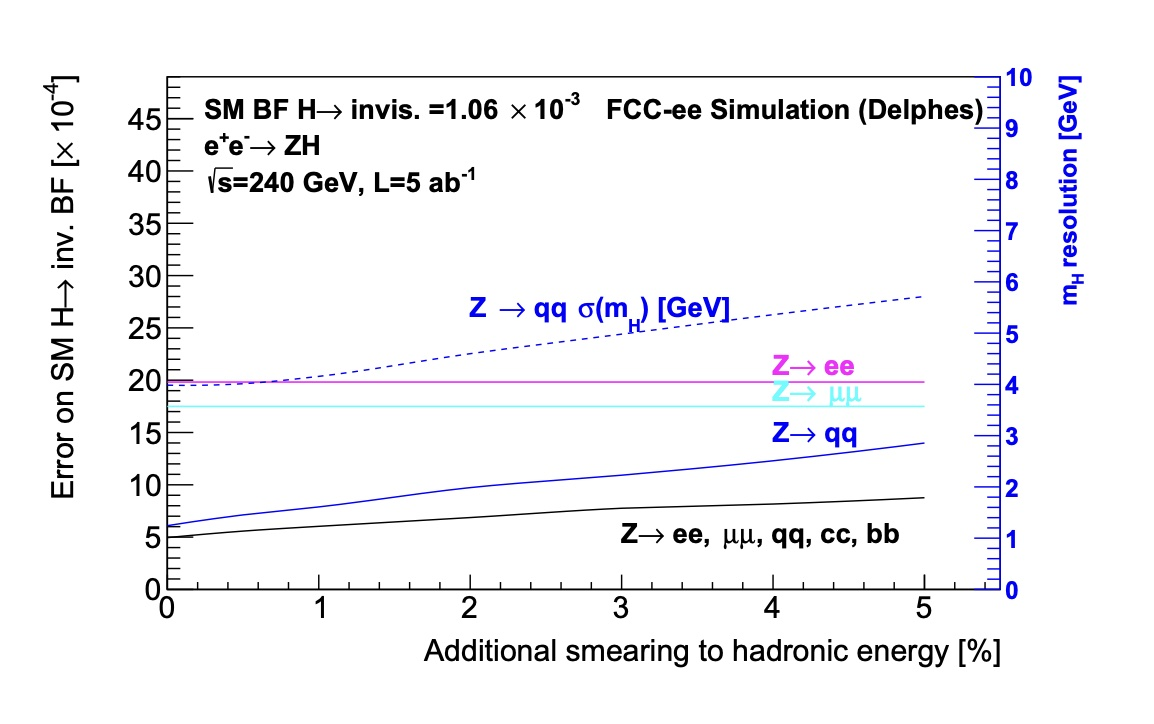
\includegraphics[width=0.8\textwidth]{DetectorRequirements/Figs/Hinv_resStudy.jpg} 
\caption{The effect of an additional smearing to the hadronic energy of the events on the expected uncertainty in a measurement of the branching fraction of the Higgs boson decay to invisible particles 
is shown for three individual channels and for all channels combined. 
The root mean squared of the reconstructed Higgs boson mass is also shown, as a dashed blue line (corresponding to the vertical axis on the right side).}
\label{fig:Hinv_resStudy}
\end{figure}

\subsubsection{Search for heavy neutral leptons}

It has been shown in Refs.~\cite{Ellis:2691414, Verhaaren_2022} that an $\epem$ machine like FCC-ee, with the potential to collect a vast event sample at the \PZ peak
holds significant discovery potential for feebly interacting particles, such as heavy neutral leptons (HNL). 
Such a large dataset, covering a phase space at low coupling strengths, is unmatched by other proposed future colliders and could potentially reach the lower bounds set by theory.
The study reported in Ref.~\cite{note_HNL_Polesello_Valle_mujj} focuses on the production of HNLs with masses between 20 and 80\,GeV at $\sqrt{s} = 91$\,GeV, 
with an integrated luminosity of $2.05\times 10^8$\,pb$^{-1}$, corresponding to $6\times 10^{12}$ $\epem \to \PZ$ events. 
In particular, the process $\epem \to N_{\PGm} \PAGnGm \to \PGm \PQq \PAQq^\prime \PAGnGm$ has been investigated. 
This process has a substantial branching ratio of about 50\% over the entire mass range of interest 
and complements other studies in the leptonic channel with long lifetimes~\cite{Verhaaren_2022,Abdullahi:2022jlv, BayNielsen:2017yws}.

In a search for HNLs that decay promptly in the detector, the analysis applies selections on muons, jets, and missing energy to minimise background contaminations. The discriminant variable used in this analysis is the visible mass, which corresponds to the HNL mass, as shown in Fig.~\ref{fig:HNLmujj_recoMass}.

The final selection involves a sliding cut on the search HNL mass, taking into account the observed resolution ($\sigma = 20\% \sqrt{m_{\text{HNL}}}$). 
A study to evaluate the impact of varying the mass resolution has been performed and the result is shown in Fig.~\ref{fig:HNLmujj_ResScan}, 
indicating a minimal effect at low masses, where the background from $\PZ \to \PQq\PAQq$ events is negligible, 
but becoming more relevant at higher masses, where the background is higher.

\begin{figure}[ht]
\centering
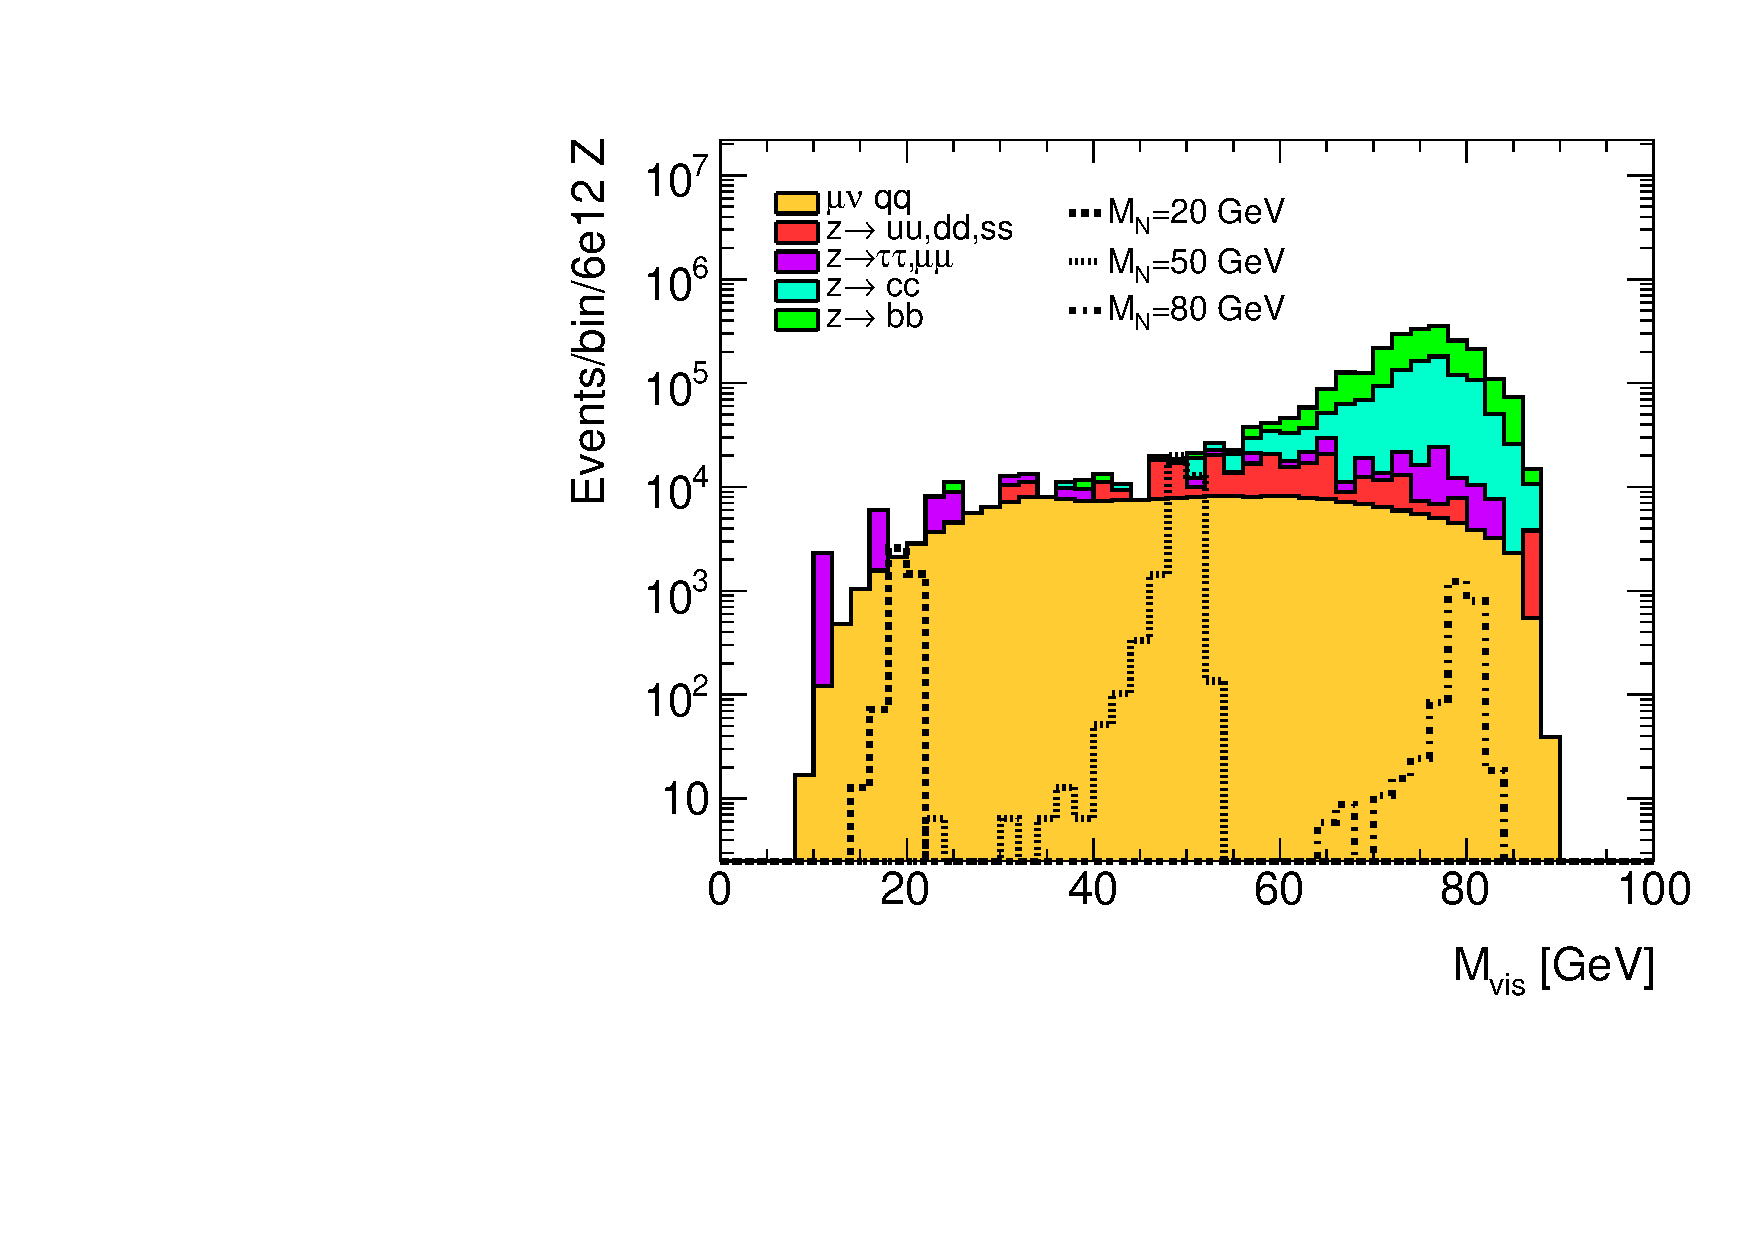
\includegraphics[width=0.8\textwidth]{DetectorRequirements/ECALFIG/Mvis_selection-CL.pdf} 
\caption{The $M_\text{vis}$ distribution for background and HNL signal events after a preliminary selection.}
\label{fig:HNLmujj_recoMass}
\end{figure}

\begin{figure}[ht]
\centering
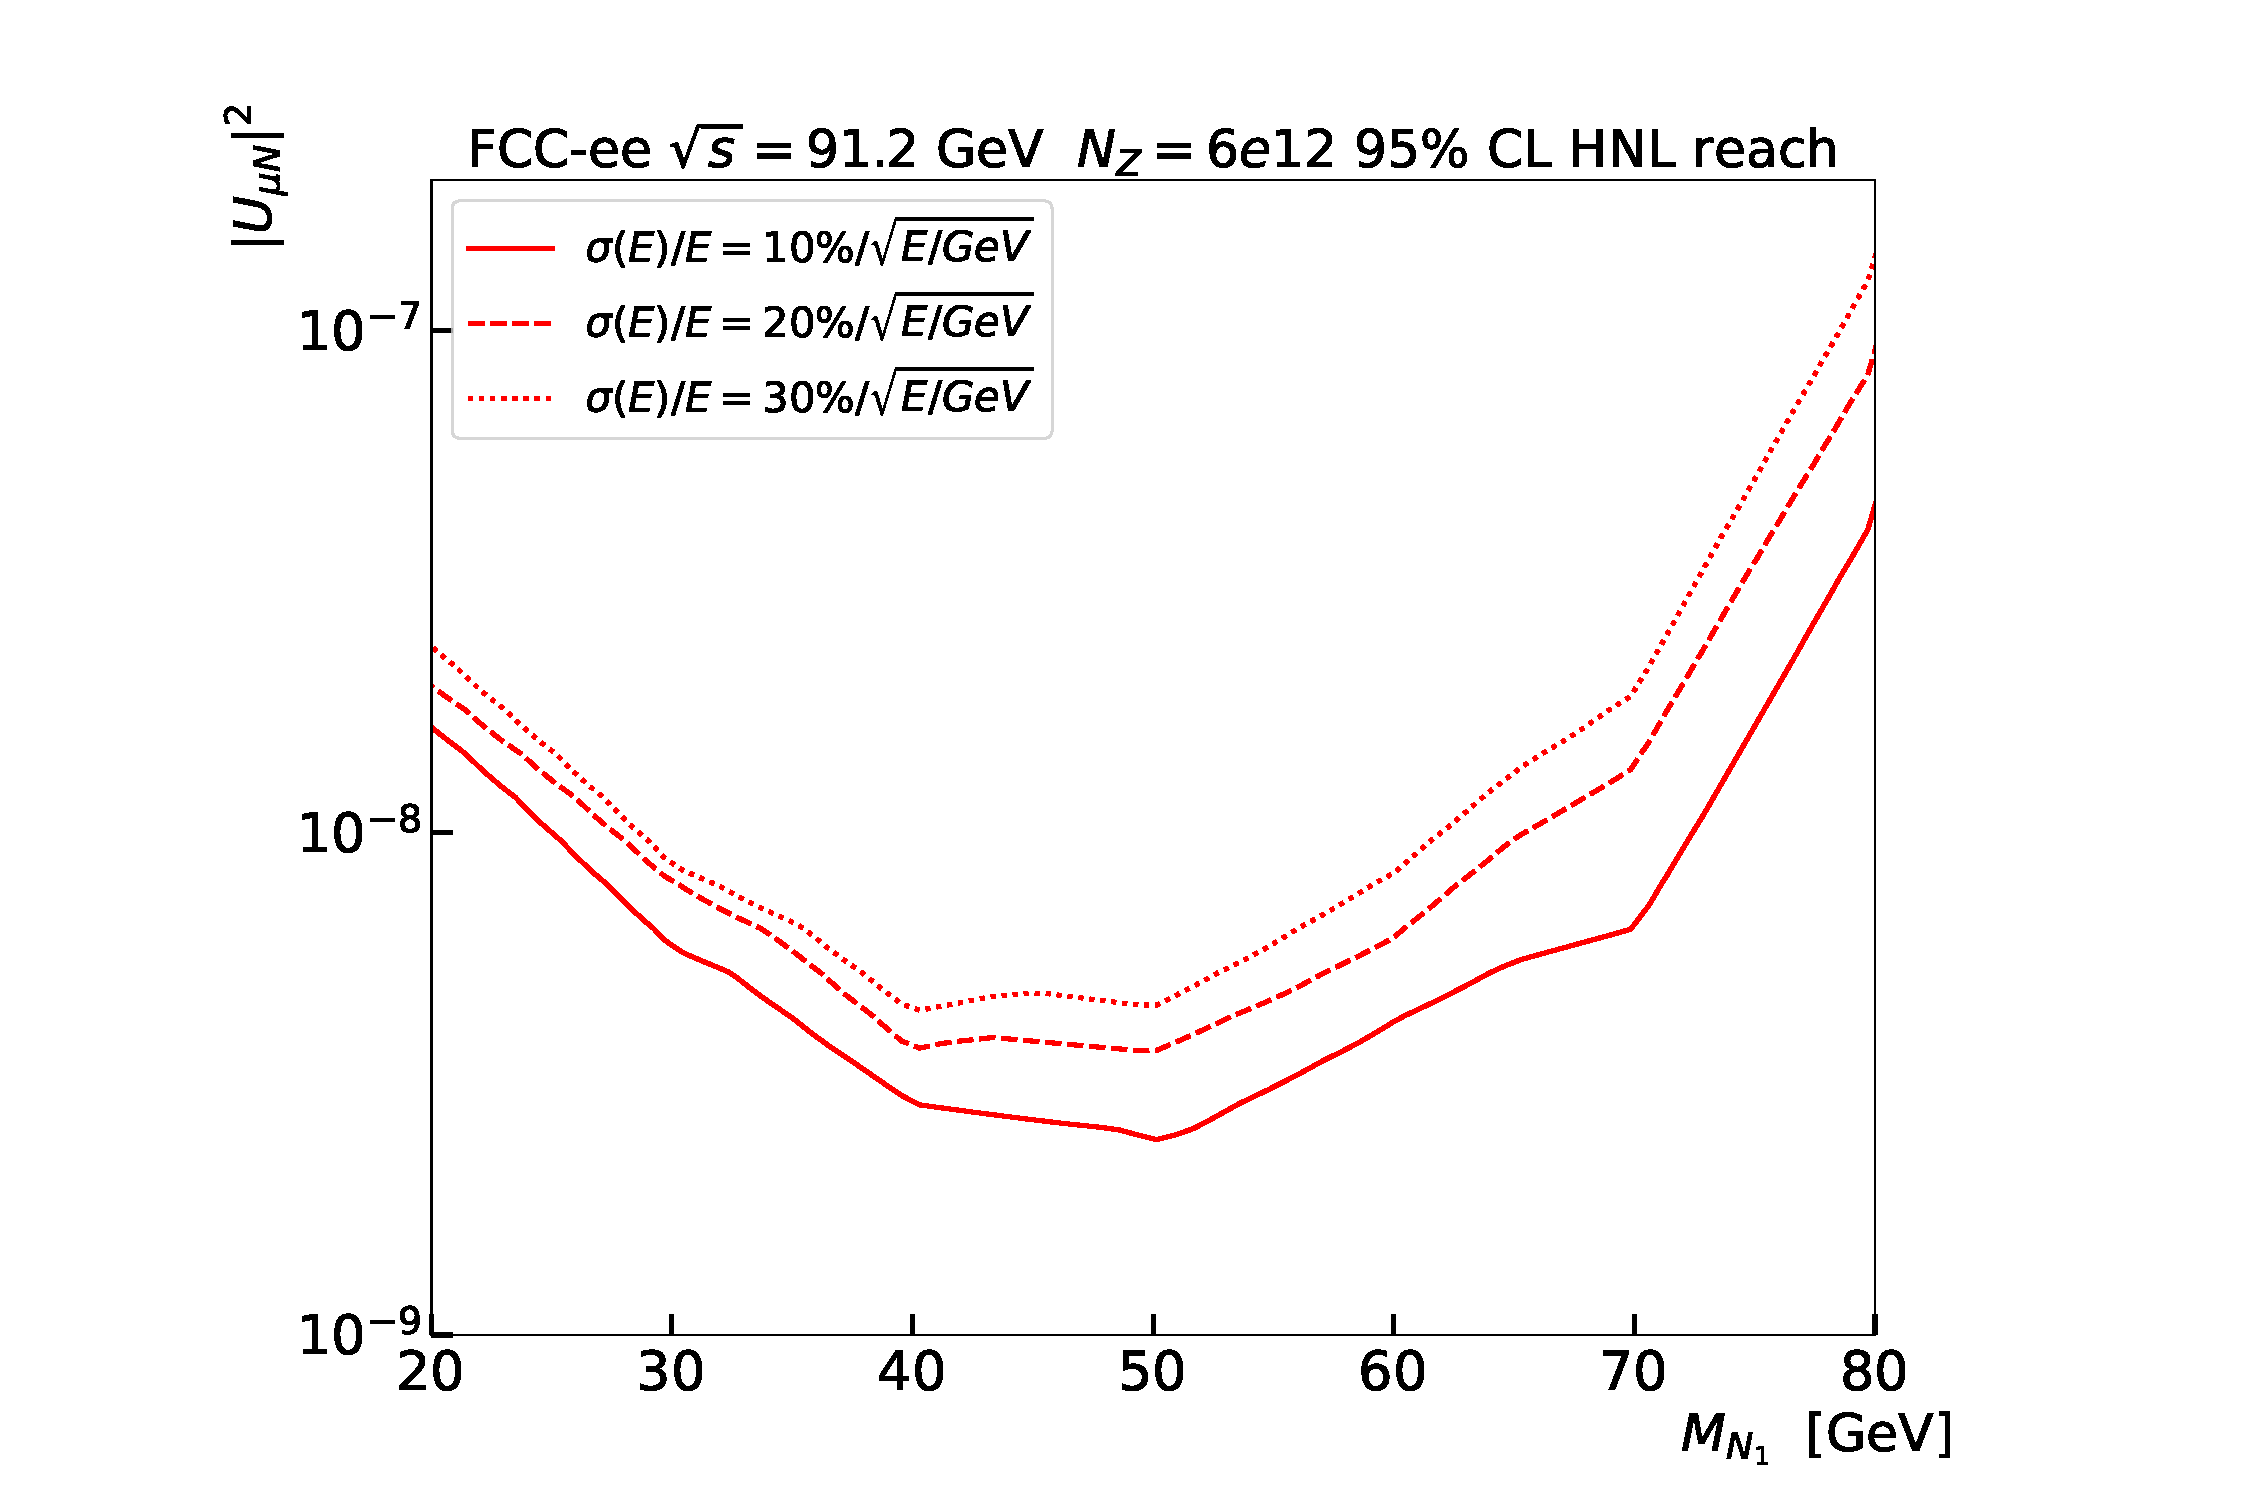
\includegraphics[width=0.7\textwidth]{DetectorRequirements/ECALFIG/res102030.pdf} 
\caption{The 2\,$\sigma$ significance of an HNL signal for several visible mass width resolutions, from a search for HNLs that decay promptly into a muon and two jets.}
\label{fig:HNLmujj_ResScan}
\end{figure}

\subsubsection{Work ahead}

\begin{itemize}

\item The total Higgs boson width measurement at $\sqrt{s} = 240$\,GeV is statistically limited by the precision on the $\PH \to \PZ\PZ^{*}$ partial width, 
which crucially depends on identifying all the hadronic \PZ decay modes. 
The separation of the \PW and \PZ mass peaks is driven by hadronic resolution and is required in order to suppress the overwhelming $\PH \to \PW\PW^{*}$ background. 
The current detector proposals satisfy this requirement in fast simulation studies, 
but this result has to be confirmed by constrained kinematic fits in full-simulation studies. 

\item These preliminary studies have been performed using a fast simulation of the detector with close to ideal particle-flow performance and can, therefore, 
only provide overall guidelines for the needed hadron calorimeter resolution.

Full-simulation performance studies with particle-flow reconstruction using integrated tracking, ECAL, and HCAL information, 
and kinematic fits constrained by the total energy and momentum conservation, 
are of paramount importance to consolidate the requirements on hadronic calorimeter technology, 
transverse and longitudinal granularity, and resolution. 

\end{itemize}

\subsubsection{Preliminary conclusions}

\begin{itemize}

\item The precision of the Higgs boson couplings to quarks and gluons, in particular the strange and charm Yukawa couplings, 
as well as the Higgs to invisible one, drives the hadron calorimeter requirements. 
Heavy neutral lepton hadronic decay modes also benefit from excellent visible energy resolution.

\item In particular, assuming an ideal particle-flow reconstruction setup with highly-efficient tracking and neutral hadron identification capabilities, 
the neutral hadron resolution drives the sensitivity to the strange Yukawa coupling. 
An excellent visible mass resolution, obtained through particle-flow reconstruction, is of paramount importance for the observation of this mode.  
\end{itemize}

\subsection{Requirements for the muon detector}
\label{sec:PhysPerf_muons}

At the FCC-ee energies, the muon momentum reconstruction is entirely driven by the tracking system 
and the main role of the muon detector is to identify muons with a very high efficiency and purity, 
as well as to serve as `tail-catcher' for the hadron showers that may not be fully contained in the calorimeter. 
An important figure of merit is the probability that a pion be misidentified as a muon.
An example benchmark measurement to set a requirement on the control of the pion contamination is that of the ultra-rare $\PB \to \PGmp\PGmm$ decay. 
As illustrated in Fig.~\ref{fig:muons_b2mumu}, the excellent mass resolution of the IDEA detector offers a very good separation of the \PB and \PBs peaks. 
A significant background coming from $\PB \to \PGpp \PGpm$ decays is, however, present under the \PB peak. 
Assuming a double $\PGp \to \PGm$ mis-identification probability of $2 \times 10^{-5}$, 
this background contribution (dashed histogram in Fig.~\ref{fig:muons_b2mumu}) would be as large as the signal~\cite{Monteil:2021ith}. 

\begin{figure}[ht]
\centering
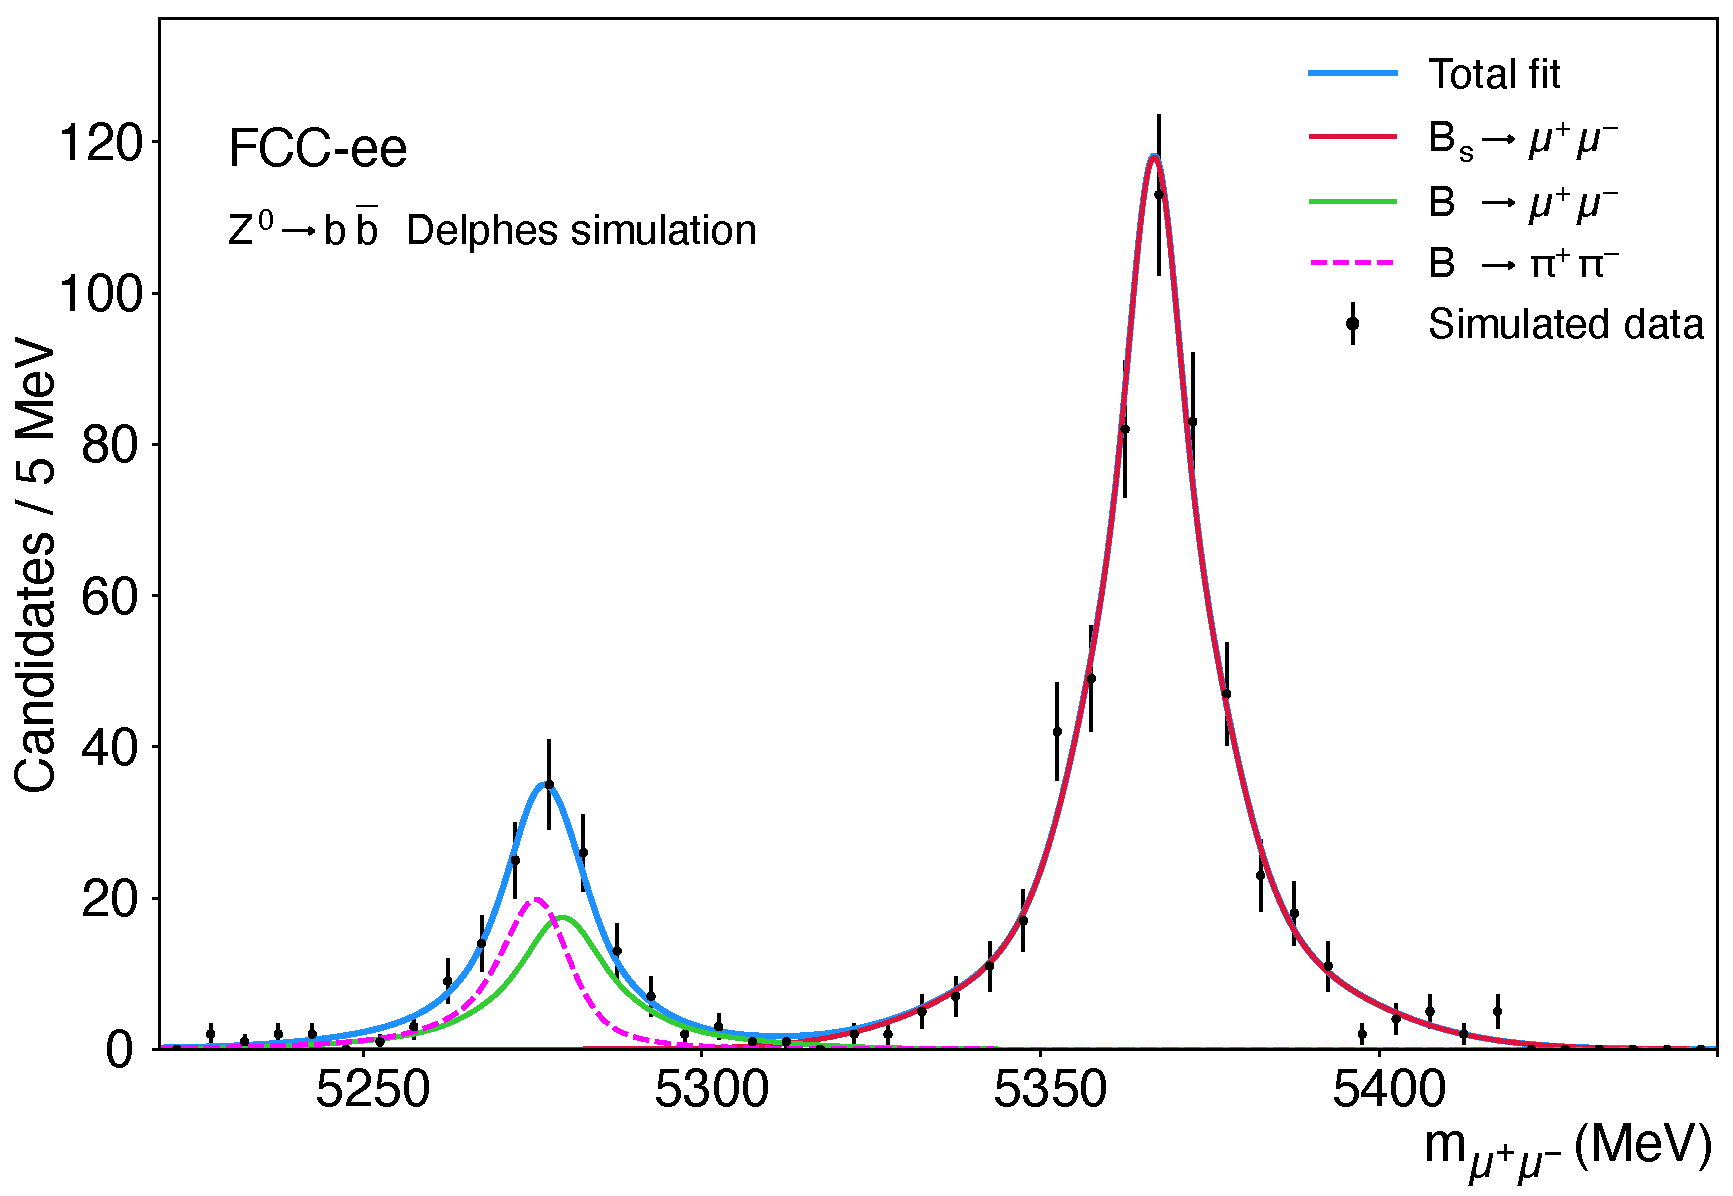
\includegraphics[width=0.7\textwidth]{DetectorRequirements/Figs/btomumu-CL.pdf} 
\caption{Mass distribution of $\PB \to \PGmp\PGmm$ and of $\PBs \to \PGmp\PGmm$ as expected from the IDEA detector, 
with an event sample of $5 \times 10^{12}$ \PZ decays. 
The background contribution from misidentified pions in $\PB \to \PGpp\PGpm$ decays is also shown, as the dashed curve. 
From Ref.~\cite{Monteil:2021ith}.}
\label{fig:muons_b2mumu}
\end{figure}

While the measurement of the track momentum in the muon detector alone does not improve (in the momentum range of interest) 
the excellent prompt muon momentum resolution already provided by the tracker, 
a good standalone resolution is useful to reduce the pion contamination and to identify pions that decay before the muon detector. 
In addition, the standalone performance of the muon detector is important in searches for long-lived particles that decay outside the tracker volume. 
The requirements on the standalone momentum resolution need to be quantified and 
they are likely to have a significant impact on the technologies that will be chosen for the muon system of an FCC-ee detector~\cite{Braibant:2021wts}.

The FCC-ee could uniquely probe yet another suppressed $\PQb \to \PQs$ transition, via the $\PBs \to \PGn \PAGn$ decay mode~\cite{Alonso-Alvarez:2023mgc}. 
The main backgrounds for this search are the $\PQb \to \PGt \PGn \mathrm{X}$ decays, 
where the \PGt decays semi-leptonically and the decay lepton escapes detection. 
This configuration can occur when the muon is forward or too soft to reach the muon detector. 
In this case, a calorimeter equipped to perform muon identification might help, together with a low detector magnetic field. 

\subsection{Precise timing measurements}

The motivations for timing measurements at FCC-ee are outlined in this section. 
Quantified requirements are still to be assessed for most of the use cases.

\subsubsection{Time-of-flight measurements}
\label{sec:PhysPerf_TOF}

As mentioned in Section~\ref{sec:PhysPerf_PID}, 
charged hadron particle identification relying on the specific energy loss must be complemented by other measurements in order to fill the gap around 1\,GeV, 
where the Bethe--Bloch energy loss function is close to its minimum. 
Time-of-flight measurements, for example in a layer of silicon sensors at 2\,m from the interaction point, with a non-challenging resolution $\sigma_t \simeq 100$\,ps, 
are adequate for this purpose (with a magnetic field of 2\,T or less). 
With a resolution of 30\,ps, such (standalone) TOF measurements would allow charged kaons to be separated from charged pions up to ${\cal{O}}$(3)\,GeV in momentum, 
while an excellent resolution of 10\,ps would be 
needed\,\footnote{Such a resolution is smaller than the time it takes, at the \PZ peak, for the two bunches to cross each other (about 36\,ps). 
Hence, to be able to exploit a 10\,ps resolution, the `event time', $t_0$, would need to be reconstructed. 
Simple algorithms should allow this $t_0$ to be reconstructed, for most SM processes, 
with a resolution of $\sigma_t / \sqrt{N}$ for events with $N$ primary tracks that reach the timing layer.} 
to extend this momentum range up to 5\,GeV.  

Such TOF information could also be obtained in a silicon-tungsten CLD-like ECAL, 
where measurements could be made in several layers, each with a resolution of, e.g., $\sim$\,100\,ps. 
Dedicated timing layers made of inorganic scintillator offer another solution. 
For example, the calorimeter design proposed in Ref.~\cite{Lucchini:2020bac} includes two such thin layers, upstream of the crystal-based ECAL mentioned earlier, which could provide a 20\,ps timing resolution.  

Another well-known use-case of TOF measurements is the determination of the mass and lifetime of new massive particles. 
An example is provided by feebly coupled heavy neutral leptons that could be copiously produced in $\PZ \to \PGn \mathrm{N}$ decays at Tera-\PZ. 
In such decays, the energy of the new lepton $\mathrm{N}$ depends only on its mass. 
In subsequent decays, such as $\mathrm{N} \to \PZ (\ell \ell) \PGn$ or $\mathrm{N} \to \PW(\PQq\PAQq^\prime) \ell$, 
the flight distance of $\mathrm{N}$ is obtained from the decay vertex of the \PZ boson 
and the TOF of the charged particles provides the time at which $\mathrm{N}$ decayed, 
from which both the lifetime and the velocity (hence the mass) of $\mathrm{N}$ can be extracted~\cite{Blondel:2022qqo}.
The need for a large tracking volume, as well as a timing resolution in the ballpark of a few tens of picoseconds, 
has so far placed the practical realisation of this idea out of realistic experimental reach.
A first study of the expected performance of this measurement technique has been presented in Ref.~\cite{Aleksan:2024hyq}, in the context of FCC-ee. 
It uses as a benchmark the process $\epem \to \mathrm{N}_{\PGm} \PAGnGm \to \PGm \PQq\PAQq^\prime \PAGnGm$, 
already considered in Section~\ref{sec:PhysPerf_HadCal}.
A simple algorithm has been developed that allows the reconstruction of the time when $\mathrm{N}$ decays, 
despite the fact that the masses of the charged particles produced in the hadronic \PW decay are, a priori, unknown. 
Since there is no way to determine the `event time' ($t_0$) of the collision for such interactions, with no primary tracks, 
it must be assumed that $\mathrm{N}$ was produced at the nominal beam crossing time. 
This leads to a smearing, of about 36\,ps, of the reconstructed time of flight of $\mathrm{N}$, from which its velocity is derived. 
Figure~\ref{fig:HNL_timing}~(left) shows the relative resolution with which the mass of the HNL can be reconstructed with this method, 
as a function of its flight distance, for an HNL mass of 40\,GeV and several assumptions on the resolution of the timing measurements, $\sigma_t$.
The resolution is defined as the width of the interval between the 16\% and the 84\% quantiles of the reconstructed mass distribution. 
The aforementioned smearing prevents reaching the ideal resolution that would be obtained with $\sigma_t = 10$\,ps, if the event $t_0$ was known, 
represented by the lowest curve in Fig.~\ref{fig:HNL_timing}~(left). 
From the two upper curves it can be seen that, provided $\sigma_t$ is smaller than 50\,ps, the degradation due to the detector resolution is limited to 20\%.
For an HNL of mass 40\,GeV that decays at 1.5\,m from the interaction point, this technique provides a mass resolution below 1\%, 
which is significantly better than what can be obtained by measuring the visible mass in the detector. 
The right panel of Fig.~\ref{fig:HNL_timing} shows that, in the parameter space that FCC-ee can probe and that extends beyond the sensitivity of the HL-LHC, 
timing measurements with $\sigma_t = 30$\,ps would allow the HNL mass to be reconstructed at the per-cent level.

\begin{figure}[t]
\centering
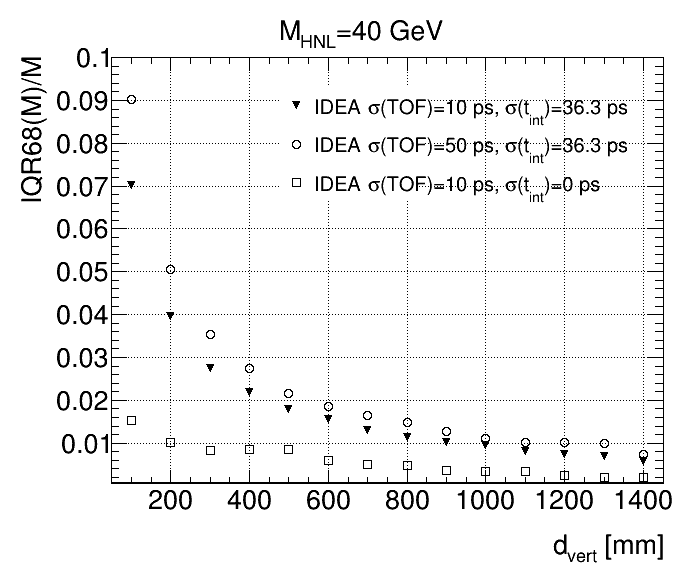
\includegraphics[width=0.46\textwidth]{Physics/DetectorRequirements/Figs/HNL_timing_resvert.png} 
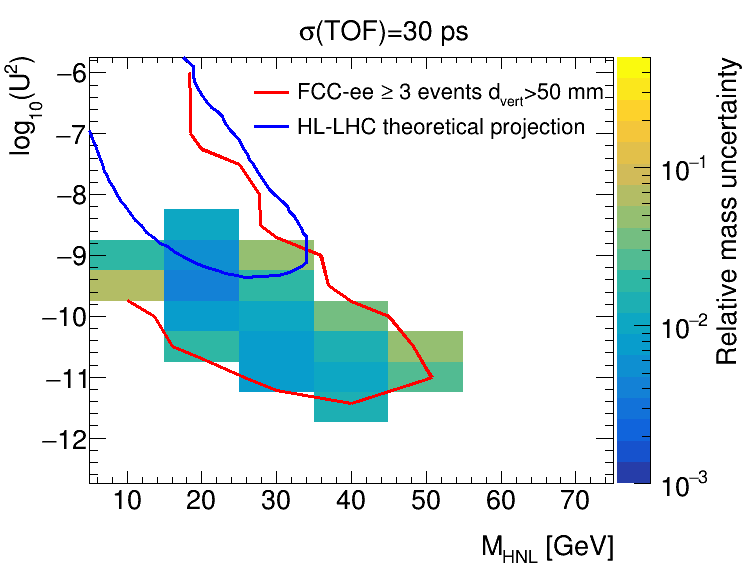
\includegraphics[width=0.5\textwidth]{Physics/DetectorRequirements/Figs/HNL_timing_bootmap.png}
\caption{Left: Relative mass resolution of the HNL as a function of its flight distance, for an HNL mass of 40\,GeV, 
using a reconstruction technique exploiting timing measurements; 
two hypotheses on the resolution of the timing measurements are considered ($\sigma_t = 10$ and 50\,ps). 
Right: Relative mass resolution expected at FCC-ee, as a function of the HNL mass and of its (squared) mixing with the $\PGnGm$, 
in the parameter space where FCC-ee could make a discovery, for a timing resolution of 30\,ps.}
\label{fig:HNL_timing}
\end{figure}

It should be noted that, should the magnetic field be increased to 3\,T (as could be considered for the runs at $\sqrt{s} = 240$\,GeV and beyond), 
particles with a momentum of 1\,GeV may not reach the outer radius of the
tracker\footnote{Prompt particles with a curvature radius $\rho$ are confined to radial distances below 2\,$\rho$ and, hence, 
need to have a transverse momentum 
$\pt \, (\text{GeV}) > 0.3 \times R  \, (\mathrm{m}) \times B \, (\mathrm{T}) / 2$ 
to reach a barrel layer situated at a radius $R$. 
Particles with a momentum of 1\,GeV and a polar angle of 45$^{\circ}$ only reach $R \sim 1.6$\,m in a 3\,T magnetic field.} 
of about 2\,m. 
Hence, to provide PID capabilities in the momentum range around 1\,GeV, where the measurement of ionisation energy per unit length does not provide any separation, 
the TOF measurements should be made either at a smaller radius  
or when the particle eventually reaches the endcaps. 
In the latter case, in particular at normal incidence, 
it is essential to investigate the effects of multiple scattering and energy loss resulting from interactions with the beam pipe and the tracker material. 
While this may pose less of an issue for a gaseous tracker, it remains important to study this aspect in detail.
In the former case and for the IDEA detector, 
the outermost layer of the vertex detector, at a radius of 35\,cm from the beams, could be used for that purpose, at the expense of an increased material budget. 
With a time resolution of 30\,ps, such standalone TOF measurements would ensure a $\PK / \PGp$ separation larger than 3\,$\sigma$ in the whole momentum range 
where PID based on d$N$/d$x$ is ineffective. 
The impact that the larger material would have on the measurement of the track parameters remains to be studied. 
In a detector design with a full silicon tracker, the TOF measurements could be made in one of the layers of the outer tracker.

\subsubsection{Time measurements very close to the IP}

At FCC-ee, the distribution of the `event time' ($t_0$) of the collisions follows a Gaussian distribution to a very good approximation, 
with a width ranging between 36\,ps during the Tera-\PZ run and 6.5\,ps during the $\ttbar$ threshold run.
The arrival time of a particle in the innermost layer of the vertex detector depends only minimally on its nature (\PK, \PGp, \PGm, \Pe, etc.), 
such that a measurement of this time provides (for primary particles) a measurement of the particle production time and of the event time $t_0$. 
For a given resolution of each measurement, $\sigma_t$, the event $t_0$ can then be determined with a resolution of $\sigma_t / \sqrt{N}$, 
with $N$ being the number of charged primary particles crossing this layer. 
Measuring the event $t_0$ offers several advantages, as listed below.

\begin{itemize}

\item It provides a robust reference for some of the TOF measurements outlined above. 

\item The spread of the $t_0$ distribution being proportional to the beam energy spread, its measurement provides an independent determination of the latter.

\item Because of the crossing angle, the $t_0$ of a collision and the longitudinal position of the colliding particles within their respective bunch are correlated. 
With respect to a time origin, defined as the time when the centres of the two bunches coincide with the IP, collisions that occur early (late) always involve particles that are in the head (tail) of both bunches. 
Collisions that happen at a time close to the origin involve particles that are in the middle of the bunches. 
Splitting the events into early, central, and late collisions can provide relevant accelerator-related information. 
For example, the mass distribution of dimuon events at Tera-\PZ would provide a check that there is no unexpected difference in the centre-of-mass energy between head and tail collisions. 
Alternatively, the longitudinal boost distribution of dimuon events at $\sqrt{s} = 125$\,GeV would exhibit a correlation~\cite{JanotEPOLtalk} 
between the centre-of-mass energy and the longitudinal position that could improve the effective monochromatisation (Section~\ref{sec:epol}). 
Moreover, further checks of the beam-beam effects could be made, 
by exploiting the fact that these effects depend strongly on the longitudinal position of the colliding particles~\cite{myTalkatKrakow}.

\end{itemize}

Moreover, the measurement of the production time of the particles complements the spatial reconstruction of primary vertices in view of a direct pile-up measurement 
(expected to be at the per-mil level at Tera-\PZ). 
However, achieving precise timing measurements in the innermost layer of the VXD, without heavily compromising the material budget, will probably be a challenge.

\subsubsection{Time measurements in the calorimeters}

Besides the TOF measurements mentioned earlier, time measurements in the calorimeters provide handles to exploit the shower development in space and time. 
The hadronic energy reconstruction, in particular in a non-compensating calorimeter, as in the CLD design, can benefit greatly from such measurements, 
which allow the delayed signal from neutrons to be identified. 
The possible benefit of timing for pattern recognition in high-granularity imaging calorimeters remains to be studied in detail. 

Finally, in the DR calorimeter of IDEA, a Fourier transform of the full signal from the SiPMs reading out the fibres would provide high precision (better than 100\,ps) timing for the individual fibres and, 
in turn, longitudinal segmentation; 
the potential benefit in a particle-flow reconstruction algorithm adapted to the hybrid segmented crystal and fibre dual-readout calorimeter of Ref.~\cite{Lucchini:2020bac} remains to be studied. 
It could also benefit the identification of low energy neutral hadrons, potentially providing neutron vs.\ \PKL separation, 
assuming that the initial time $t_0$ is known. 
However, a concrete implementation has to be studied in detail.

\subsection{Selected studies with full simulation}
\label{sec:PhysPerf_FullSim}

Most of the requirements discussed in the previous sections have been obtained using fast parametrised simulations. 
While a full simulation and event reconstruction with every detector concept is beyond the scope of this feasibility study, 
a few selected preliminary reconstruction performance and physics results obtained with full simulation are presented in this section. 
With the exception of ML-based tracking, all of them use the reconstruction of the CLD detector concept. 
A high-level machine-learning-based particle-flow reconstruction algorithm is first discussed. 
An initial implementation of a full simulation flavour tagging algorithm in CLD is described next and the achieved performance is compared with the fast simulation results. 
Finally, the Higgs mass measurement using the recoil mass method and the \PGt polarisation measurement at the \PZ pole are addressed.

\subsubsection{Machine-learning event reconstruction}

The Higgs boson decays preferentially into hadrons. 
Therefore, the optimal identification and reconstruction of hadronic jets is crucial for measuring Higgs boson properties. 
In particular, resolving the mass peaks from $\PW, \PZ \to jj$ hadronic decays at the 3\,$\sigma$ level 
requires reconstructing the dijet masses with a resolution $\sigma_m$ at the $\Gamma / m \approx 2.5\%$ level, 
where $\Gamma$ is the natural \PW or \PZ width. 
Moreover, the measurement of rare hadronic Higgs decay rates, such as $\PH \to \PQc\PAQc$ and $\PH\to \PQs\PAQs$, 
requires excellent dijet mass resolution, since the relative uncertainty on these modes scales with $\sqrt{\sigma_m}$, 
as discussed in Section~\ref{sec:PhysPerf_HadCal}.

The visible energy of hadronic jets is roughly distributed as follows: 
$f_{\pm} = 65\%$ from charged hadrons (\PGppm, \PKpm, \ldots), 
$f_{\PGg} = 25\%$ from photons originating from \PGpz decays, 
and $f_\mathrm{n} = 10\%$ from neutral hadrons (\Pn, \PKL, \ldots). 
The particle-flow approach relies on the tracking system to measure the momenta of charged particles, benefiting from its superior resolution, compared to the calorimeters, 
while the energies of photons and neutral hadrons are measured with the calorimeters. 
In an ideal PF algorithm, the visible mass resolution is dominated by the HCAL resolution, despite the neutral hadron energy content being subdominant. 
Achieving the best mass resolution requires efficiently identifying neutral hadrons and disentangling them from mismeasured clusters originating from charged hadron showers.

An optimal PF algorithm requires nearly 100\% tracking efficiency and purity over the full momentum range for an accurate measurement of the charged energy component. 
Fine transverse and longitudinal calorimeter segmentation is necessary for optimal geometrical matching of extrapolated track trajectories to electromagnetic and hadron showers. 
Additionally, low-noise high-resolution calorimetry and efficient clustering algorithms are essential for identifying and reconstructing individual photon and neutral hadron showers. 
Excellent electromagnetic and hadron calorimeter resolutions are crucial for comparing tracking and calorimeter energy measurements after geometrical matching. 
A low material budget in the tracker and before the calorimeter (e.g., pre-shower or solenoidal magnet) is desirable to minimise nuclear interactions and conversions 
that could compromise track, photon, and neutral hadron reconstruction efficiency. 
Moreover, the PF reconstruction performance depends critically on the transverse and longitudinal granularity for optimal track-cluster matching and neutral hadron identification. 
Finally, maximising the hermeticity and uniformity of the detector design is crucial for PF reconstruction.

Electron and muon identification and momentum determination, whether isolated or within jets, also benefit from a holistic treatment of all detector components~\cite{ALEPH:1994ayc,CMS:2017yfk}. 
For example, as shown in Section~\ref{sec:PhysPerf_ECAL}, photon bremsstrahlung emissions within the tracker requires combining tracking and ECAL information. 
Similarly, muons are identified by combining data from tracking, calorimetry, and muon detectors. A
comprehensive PF reconstruction should encompass a wide range of tasks, 
aiming at providing an exhaustive list of identified final-state particles produced in the collisions and interacting with the detector, 
along with accurate measurements of their momenta and origin vertices.

A novel approach to full event reconstruction based on graph neural network (GNN) methods is described in the following. 
The goal is to improve every aspect of the reconstruction process, from efficiency to resolution, 
and to enable rapid iterations over various detector concepts and geometries, so as to estimate performance and, hence, optimise detector technologies and design options. 
The effectiveness of this approach is shown in Fig.~\ref{fig:fullsim_mlreco}. 
The left panel displays the tracking efficiency achieved with machine learning (ML) methods using the \textsc{ggtf} algorithm~\cite{MLTRACKING_NOTE} 
for the CLD and IDEA detectors in $\PZ \to jj$ events at the \PZ pole. 
The ML approach significantly improves the CLD performance with respect to the standard tracking 
(a similar comparison for the IDEA case cannot be made because the baseline reference is missing). 
It also shows that IDEA, with its superior number of track measurements, can reconstruct much lower transverse momentum tracks, 
which are crucial for optimal PF reconstruction since a significant portion of the visible jet energy is carried by soft charged particles. 
The right panel illustrates the visible mass resolution in $\PZ\PH \to \PGn \PAGn \PQs \PAQs$ events at $\sqrt{s} = 240$\,GeV 
obtained with ML-based PF (MLPF) compared to the \textsc{Pandora} particle-flow reconstruction~\cite{pandorapfa,pandorasdk}, showing similar performance. 
This result was obtained using GNN-based PF reconstruction, described in more detail in Ref.~\cite{MLPF_NOTE}, 
taking as input reconstructed classical tracks and low-level calorimeter hit reconstruction. 
Although this is work in progress, it indicates that the established PF algorithm performance can already be reproduced with this approach. 
Further improvements are foreseeable by optimising the clustering step, 
enhancing the neutral hadron identification efficiency, and making use of further optimised tracking algorithms.

\begin{figure}[t]
\centering
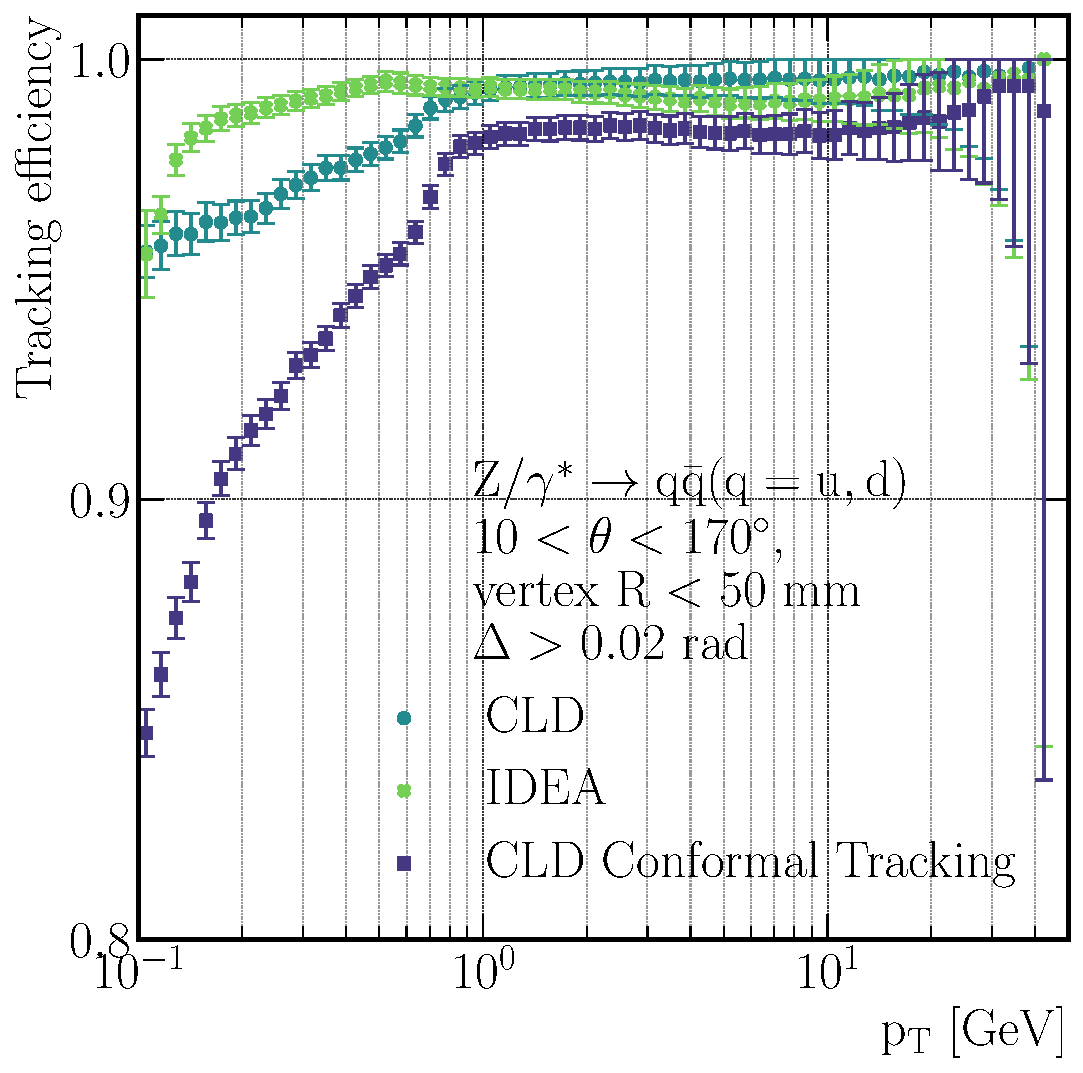
\includegraphics[width=0.495\textwidth]{Physics/DetectorRequirements/Figs/tracking_eff.pdf} 
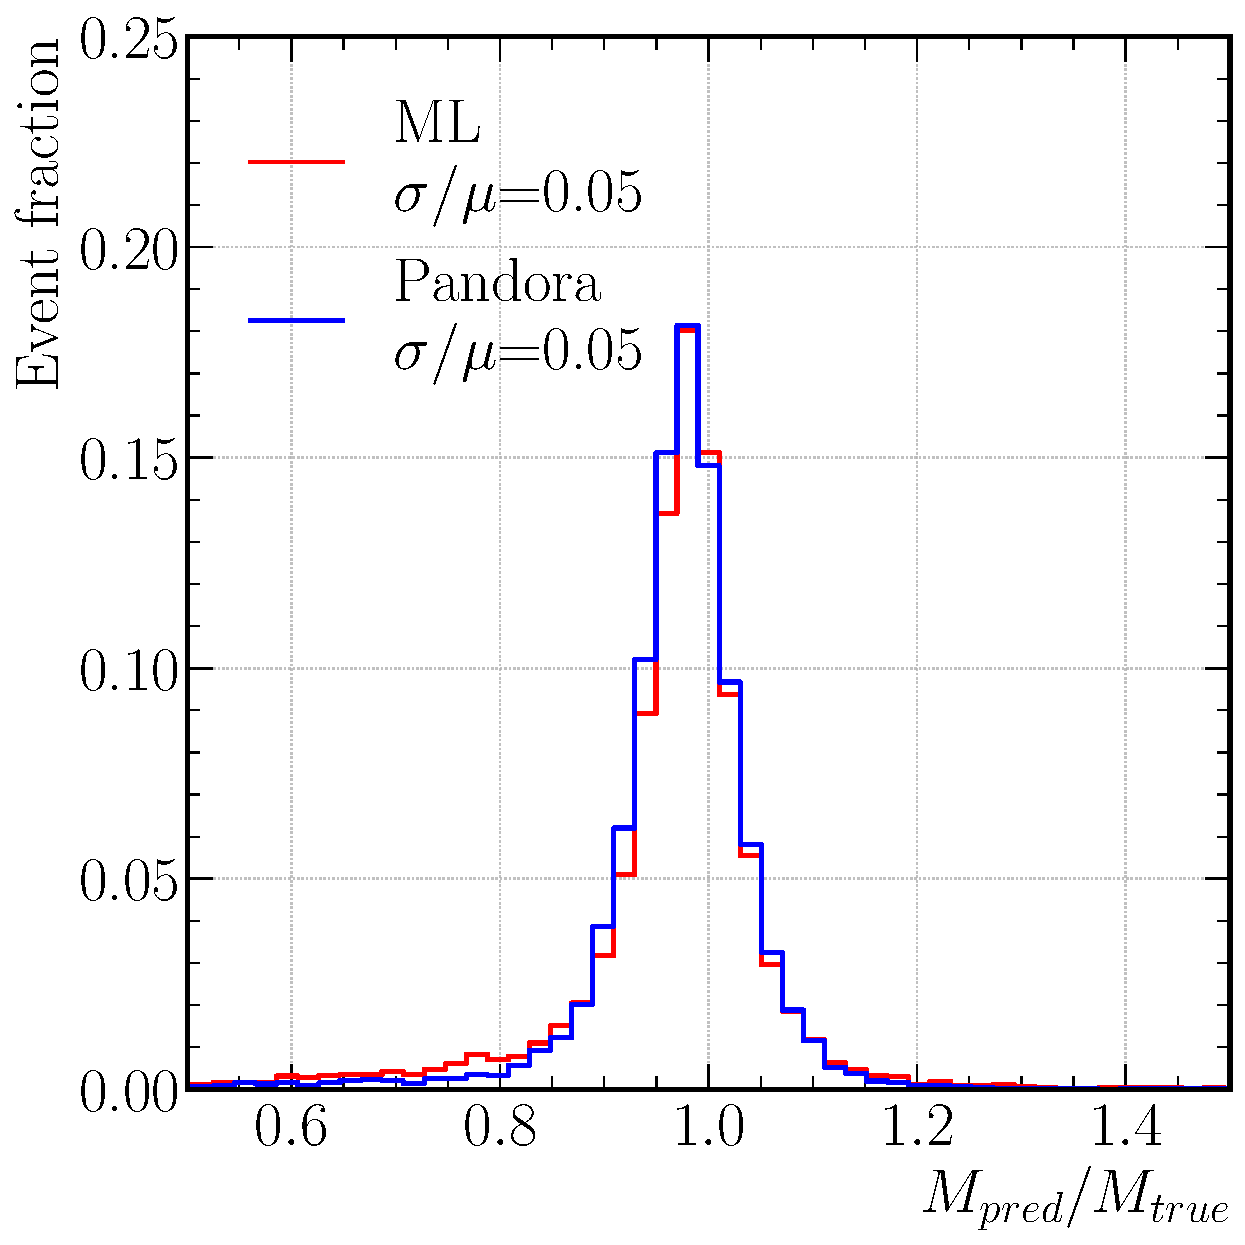
\includegraphics[width=0.495\textwidth]{Physics/DetectorRequirements/Figs/mvis_mlpf.pdf}
\caption{Left: Tracking efficiency in CLD and IDEA using the classical (Conformal Tracking) and ML-based (\textsc{ggtf}) approaches. 
Right: Visible mass resolution in $\PH \to \PQs\PAQs$ events using the classic \textsc{Pandora} reconstruction and the ML-based particle flow approach.}
\label{fig:fullsim_mlreco}
\end{figure}

\subsubsection{Jet flavour tagging}

The first investigation of jet-flavour tagging performance with a full simulation of the CLD detector concept at FCC-ee is briefly presented here, 
and discussed in more details in Ref.~\cite{TAGGINGFULLSIM_NOTE}. 
As discussed in Sections~\ref{sec:PhysPerf_Hcc} and~\ref{sec:PhysPerf_strangeTagging}, 
jet-flavour tagging is essential for precision measurements of the Higgs couplings to quarks and gluons. 
A modified \textsc{Delphes} configuration simulates the CLD detector geometry and resolutions in fast simulation, referred to as the \emph{CLD fast simulation}. 
The full simulation uses the CLD conformal tracking (the baseline tracking reconstruction in CLD) to reconstruct charged particles. 
The \textsc{Pandora} particle flow algorithm~\cite{pandorapfa,pandorasdk} is used for global event reconstruction, to build a particle-level view of the event. 

Jets are clustered with the \kt Durham algorithm~\cite{Catani:1991hj} using $N = 2$ exclusive clustering on 
$\epem \to \PZ\PH \to \PGn \PAGn j j$ events. 
The input to jet clustering are the reconstructed tracks and the neutral particles reconstructed by \textsc{Pandora}. 
The jet flavour tagger~\cite{Bedeschi:2022rnj} is then applied to assign each jet a probability of originating from a given flavour among seven possible categories: 
\Pg, \PQu, \PQd, \PQs, \PQc, \PQb, and \PGt. 
The tagger uses the information of all the input particles within a jet, including kinematic, displacement, and particle identification properties. 
Adding direct vertex information (positions and invariant masses of secondary vertices) to the network does not improve performance, 
indicating that the model effectively learns vertexing from the track displacement, the charged particle content, and the kinematic variables. 

\begin{figure}[ht]
\centering
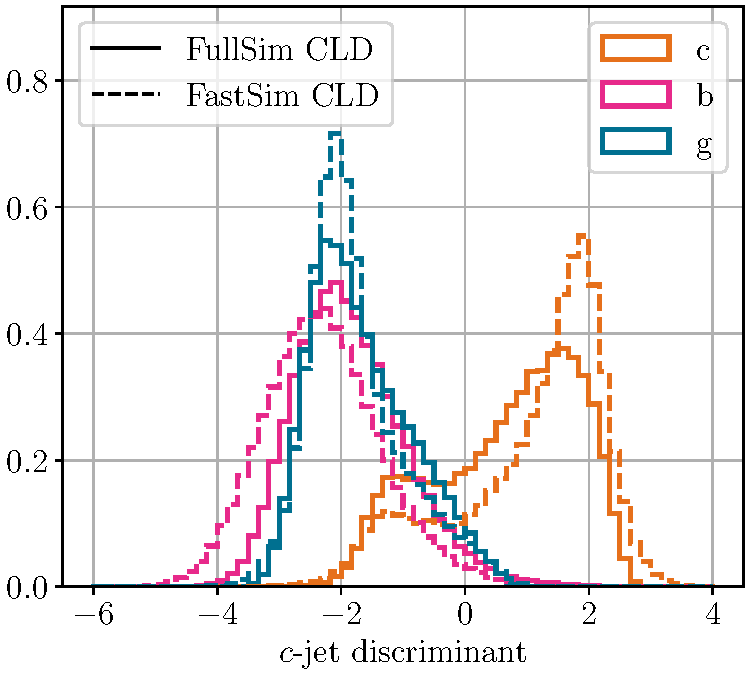
\includegraphics[width=0.48\textwidth]{Physics/DetectorRequirements/Figs/discrim-non-bi_FastSimCLD240_vs_FullSimCLDtcmatch_cjet.pdf} 
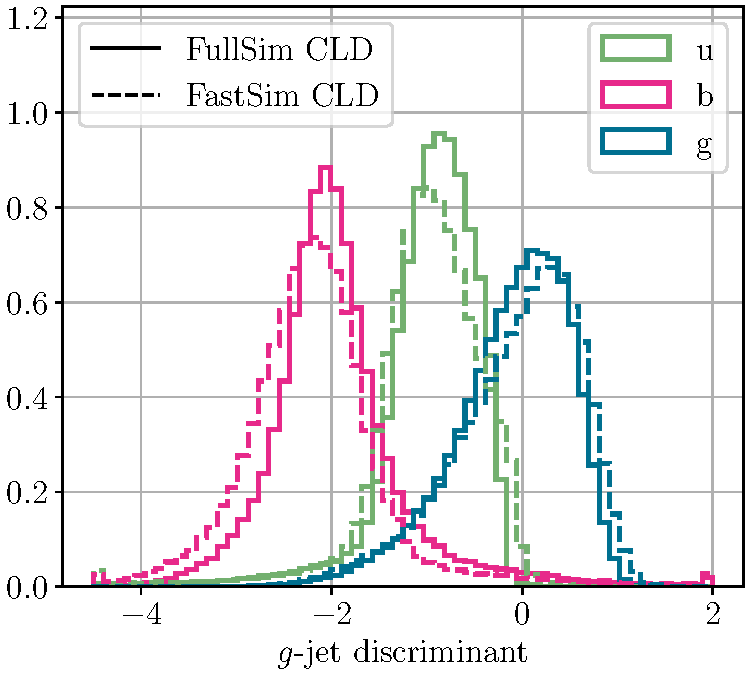
\includegraphics[width=0.48\textwidth]{Physics/DetectorRequirements/Figs/discrim-non-bi_FastSimCLD240_vs_FullSimCLDtcmatch_gjet-1.pdf} 
\caption{Flavour tagging output in the full (solid) and fast (dashed) CLD simulation for charm (left) and gluon (right) multi-variate discriminants for various jet species.}
\label{fig:fullsim_tagging}
\end{figure}

The implementation of the algorithm in \textsc{Delphes} and its performance are described in detail in Ref.~\cite{Bedeschi:2022rnj}. 
Both fast and full simulation datasets are trained using identical input features. 
For illustration purposes, Fig.~\ref{fig:fullsim_tagging} shows the charm and gluon score, 
defined as the monotonic transformation of the tagging probability $\log(P\,/\,(1-P))$. 
The fast- and full-simulation output scores agree reasonably well. 
Additional jet tagging scores and performance figures can be found in Ref.~\cite{TAGGINGFULLSIM_NOTE}.

It is observed that fast simulation features better performance across all tagging categories. 
For instance, in \PQc-tagging, the efficiency of correctly identifying \PQc-jets vs.\ misidentifying light-quark jets decreases from 80\% in fast simulation to 70\% in full simulation, 
for a 1\% light quark misidentification rate. 
This loss in performance is under investigation but can be largely explained by track reconstruction inefficiencies in full simulation and a sub-optimal particle-flow algorithm parameter tuning.

This study shows that initial jet-flavour tagging performance in full simulation in CLD is sub-optimal. 
Future work should focus on improving CLD reconstruction to mitigate the identified limitations, such as low tracking efficiency at low momentum and large neutral hadron mis-identification probability. 
In addition, exploring the use of energy loss per unit length (d$E$/d$x$) information from the silicon tracker may provide additional particle identification capabilities, 
which can be useful for strange jet identification and can also provide additional exploitable information for charm, bottom, and tau tagging. 
Making progress in these areas is crucial to achieve the FCC-ee precision Higgs physics goals.

\subsubsection{Higgs boson mass determination}

Measuring the Higgs boson mass precisely at FCC-ee is important because it constitutes a limiting parametric uncertainty in the calculations of the branching ratios of the Higgs boson decay channels. 
Achieving a precision of 4\,MeV makes this uncertainty negligible and leads to more accurate predictions of the Higgs boson decay properties. 
Also, knowing $m_{\PH}$ with a precision comparable to the Higgs boson natural width 
is the minimum requirement for potentially measuring the electron Yukawa coupling at $\sqrt{s} = 125$\,GeV, 
the Higgs boson pole (Section~\ref{sec:eYukawa}).

\begin{figure}[ht]
\centering
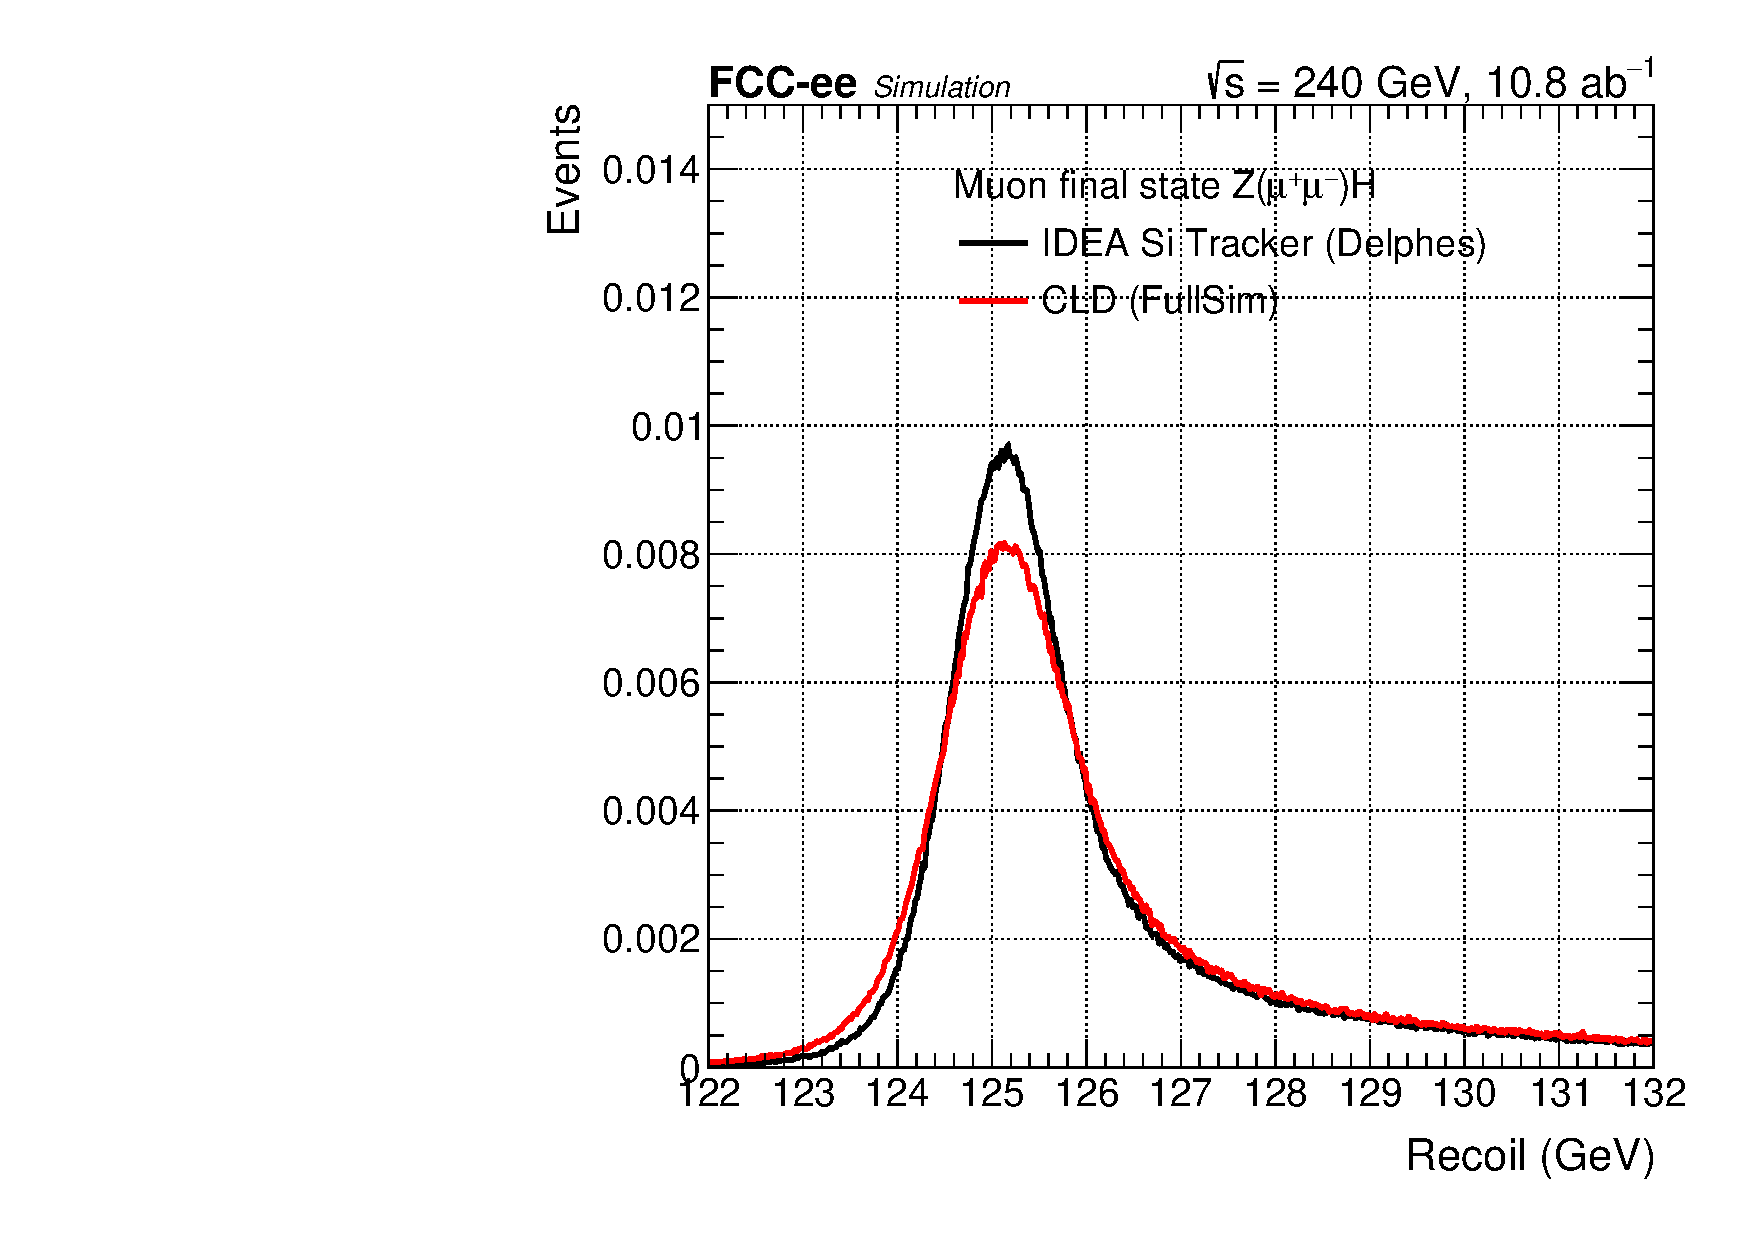
\includegraphics[width=0.48\textwidth]{Physics/DetectorRequirements/Figs/CLD_recoil.pdf}    
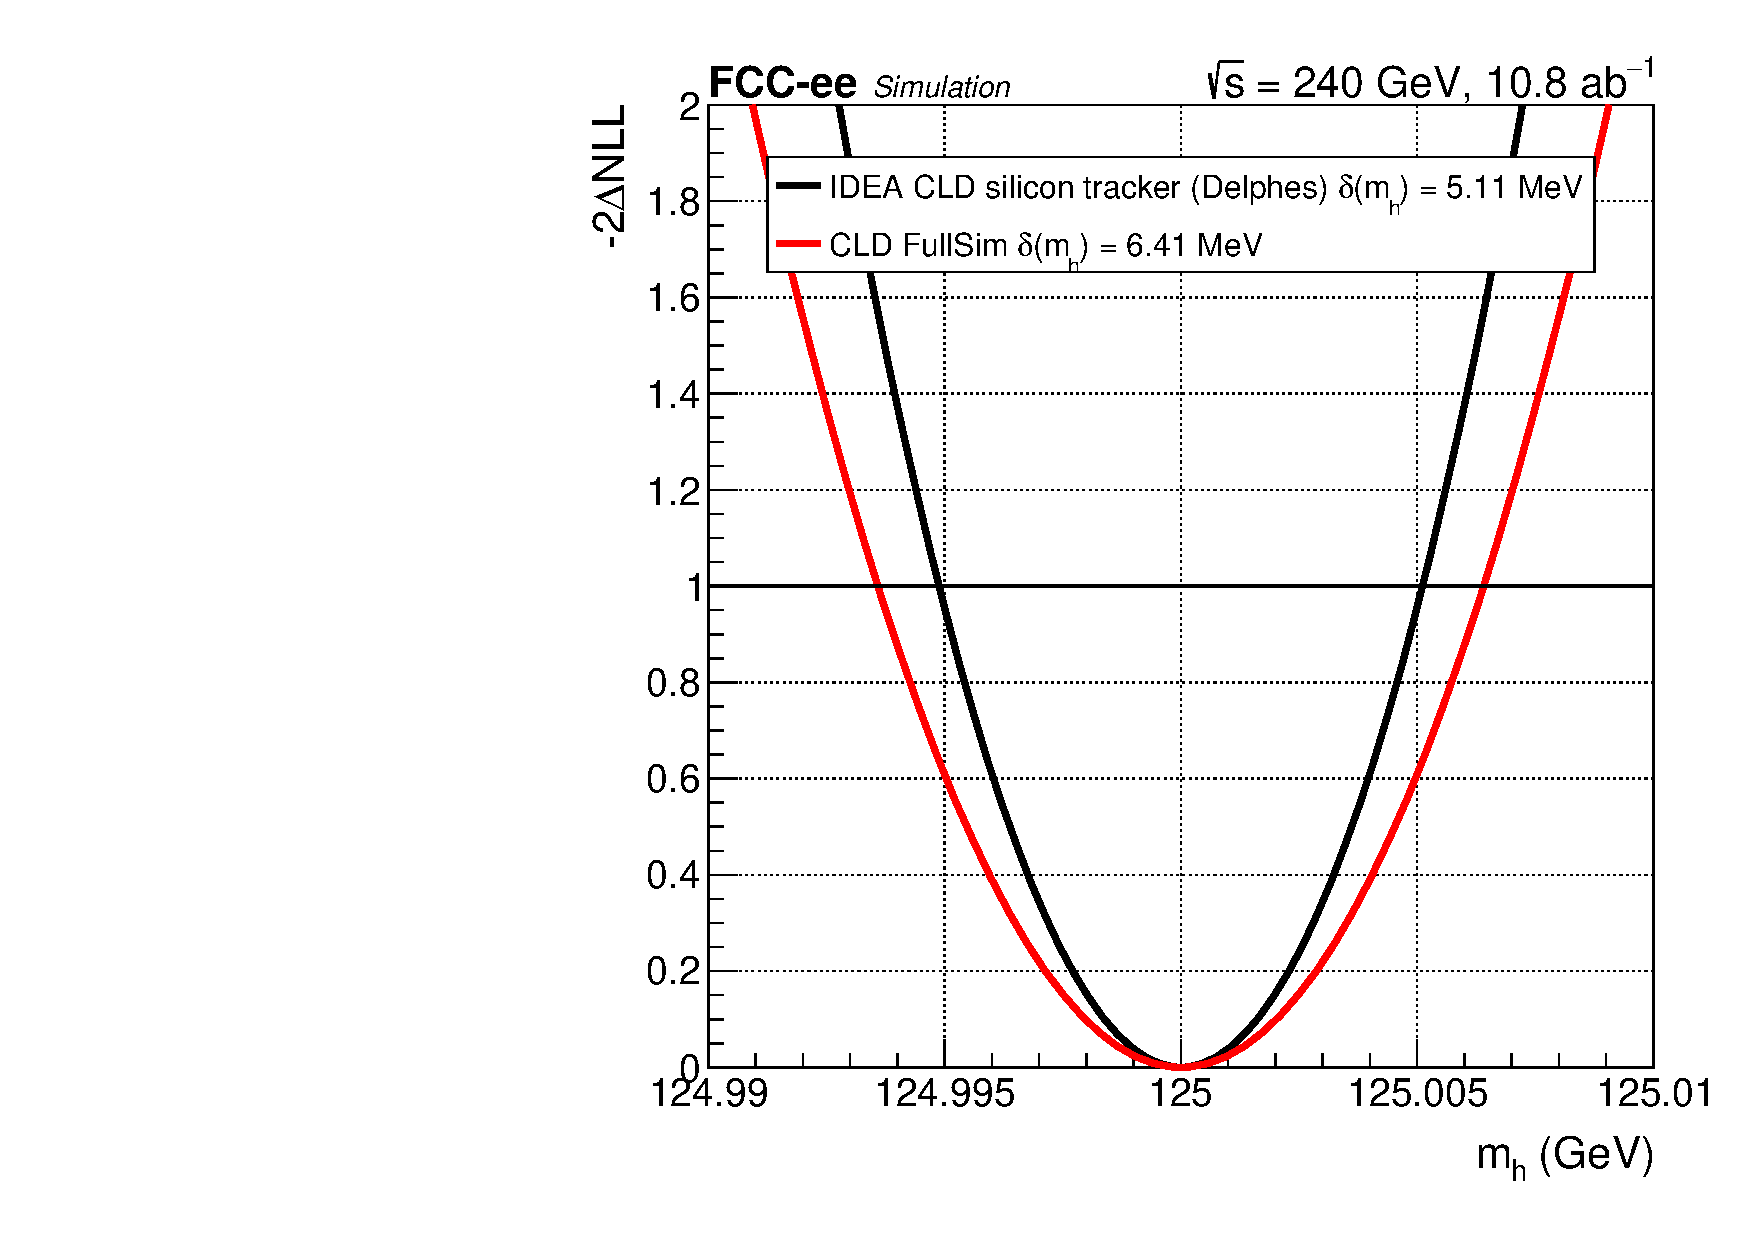
\includegraphics[width=0.48\textwidth]{Physics/DetectorRequirements/Figs/comparison_stat.pdf}
\caption{Higgs boson mass determination using the recoil mass method in the dimuon channel in the full (red curves) and fast (red curves) simulation. 
Left: The $m_\text{recoil}$ distribution. 
Right: Likelihood scan of the Higgs boson mass and corresponding precision.}
\label{fig:fullsim_mh}
\end{figure}

The Higgs boson mass measurement prospects have been studied in full simulation using the CLD detector~\cite{HiggsNoteRecoil}. 
Track reconstruction and muon identification are the main event reconstruction features required for this measurement, 
which allows a straightforward comparison to fast simulation. 
The Higgs boson mass recoil method and the resulting sensitivity obtained with fast simulation in the dimuon and dielectron channels 
are extensively discussed in Sections~\ref{sec:PhysPerf_HiggsRecoil} and~\ref{sec:PhysPerf_ECAL}, 
assuming the IDEA detector performance with a gaseous drift chamber or, alternatively, a CLD-like silicon tracker. 
The driving experimental factor for the sensitivity is the track momentum resolution, ultimately limited by the multiple scattering induced by the beam pipe and tracker material. 
A gaseous tracking device is, therefore, preferred for this measurement. 
In this study, the recoil mass method has been applied to the CLD silicon tracking full simulation and compared to the CLD-like fast simulation results, 
as shown in Fig.~\ref{fig:fullsim_mh}. 
The recoil mass distribution obtained in $\epem \to \PZ\PH \to \PGmp\PGmm \PH$ events is shown on the left panel; 
it agrees at the 15\% level with the fast simulation distribution. 
This small discrepancy is most likely explained by a small difference in the tracker material description and is currently under investigation. 
The right panel shows the corresponding precision on the Higgs boson mass determination, 
obtained from a likelihood scan using different mass hypotheses, yielding a precision of 6.4\,MeV for full simulation, 
compared to 5.1\,MeV in fast simulation.

This study shows that the full simulation of the CLD detector is available to perform a complete physics benchmark study. 
Further work is needed to understand the discrepancy in the observed precision between fast and full simulation, 
which may also point to shortcomings in the full event simulation and reconstruction. 
Extending the study to the dielectron final state, which requires the implementation of photon bremsstrahlung recovery to fully reconstruct the final-state electron momentum, 
will be an important step forward in the understanding of the CLD detector performance in this important measurement.

\subsubsection{Tau polarisation}

The \PZ-pole running will provide an unprecedented sample of $2 \times 10^{11}$ clean $\PGtp\PGtm$ events
and a unique opportunity for the determination of the tau polarisation,
which is in turn very sensitive to the electroweak couplings of the \PZ boson ($\sin^2 \theta_{\PW}$). 
The tau polarisation is defined as 
\mbox{$\mathcal{P}_{\PGt} = (\sigma_+ - \sigma_-)/(\sigma_+ + \sigma_-)$}, 
where $\sigma_+$ and $\sigma_-$ are the production cross sections of left-handed and right-handed taus, respectively. 
It can be expressed as a function of the electron and tau asymmetry parameters, $\mathcal{A}_{\Pe}$ and $\mathcal{A}_{\PGt}$, 
and it depends on the angle $\theta$ between the tau momentum and the electron beam in the centre-of-mass frame of the collision:
\begin{equation}
\mathcal{P}_{\PGt}(\cos\theta) = 
- \frac{\mathcal{A}_{\PGt} (1+\cos^2 \theta) + 2 \mathcal{A}_{\Pe} \cos\theta} 
{1+ \cos^2\theta + 2 \mathcal{A}_{\Pe} \mathcal{A}_{\PGt} \cos\theta} \, .
\end{equation}

The measurement of $\mathcal{P}_{\PGt}(\cos\theta)$ allows the determination of $\mathcal{A}_{\PGt}$ and $\mathcal{A}_{\Pe}$, 
as a test of the universality of the \PZ boson couplings to electrons and taus. 
Integrating over $\cos\theta$, one obtains $\mathcal{P}_{\PGt}^\text{total} = -\mathcal{A}_{\PGt}$. 
At LEP, the uncertainty in $\mathcal{A}_{\Pe}$ was statistically dominated~\cite{ALEPH:2005ab}, while for $\mathcal{A}_{\PGt}$ systematic and statistical uncertainties were at the same level. 
The large FCC-ee data samples and advanced detector capabilities are expected to significantly reduce these uncertainties. 
Assuming a factor 10 improvement in the systematic uncertainty with respect to LEP, the systematic uncertainty in $\mathcal{A}_{\PGt}$ could be as low as 0.02\%, 
with $\mathcal{A}_{\Pe}$ having an even smaller uncertainty.

To confirm our expectations that this precision can be achieved, 
a full simulation study of the CLD detector is underway, focusing on tau reconstruction and identification. 
Tau identification relies on reconstructing charged hadrons and photons from $\PGpz \to \PGg\PGg$ decays. 
About 65\% of tau decays are hadronic, decaying to one or three charged hadrons accompanied by photons from \PGpz decays. 
An algorithm based on the \textsc{Pandora} particle-flow candidates has been developed to reconstruct the main decay modes: 
$\PGt \to \PGp\PGn$, $\PGt \to \PGr\PGn \to \PGp\PGpz \PGn$, and $\PGt \to \Pa_1\PGn$. 
In parallel, a GNN method is being developed to improve the identification performance. 

A first analysis limited to $\PZ \to \PGt\PGt$ events in which one of the taus decays leptonically in one hemisphere and the other decays hadronically in the other hemisphere 
has been performed~\cite{alcaraz_maestre_2024_qnyyh-skw71}. 

Figure~\ref{fig:fullsim_taupol} shows the optimal variables for the three main configurations considered in the analysis. 
The first mode is designed to select $\PGt \to \PGp \PGn$ decays. 
In this case the optimal variable is directly the energy fraction  $x_{\PGp} = {E_{\PGp}} \,/\, {E_\text{beam}}$. 
The other two configurations correspond to the $\PGt \to \PGr \PGn \to \PGp \PGpz\PGn$ channel with the reconstruction of either one or both of the \PGpz decay photons. 
Here the optimal observable at LEP was defined to be
\begin{equation}
\omega_{\PGr} = \frac{W_+(\theta^*, \psi) - W_-(\theta^*, \psi)}{W_+(\theta^*, \psi) + W_-(\theta^*, \psi)} \, ,
\end{equation}
where $W_+$ and $W_-$ represent the angular distributions of the \PGr decay products for different helicity states, 
and $\theta^*$ and $\psi$ are angles describing the decay products in the \PGt rest frame~\cite{Nikolic:1996nj}. 
The reweighted $\mathcal{P}_{\PGt} = \pm 1$ signal templates are shown in comparison to the SM prediction. 
Additionally, the backgrounds coming from tau misidentification are also shown. 
No other backgrounds are considered at this stage. 
Further studies of the full simulation samples and optimisation of the reconstruction algorithm are in progress. 

\begin{figure}[ht]
\centering
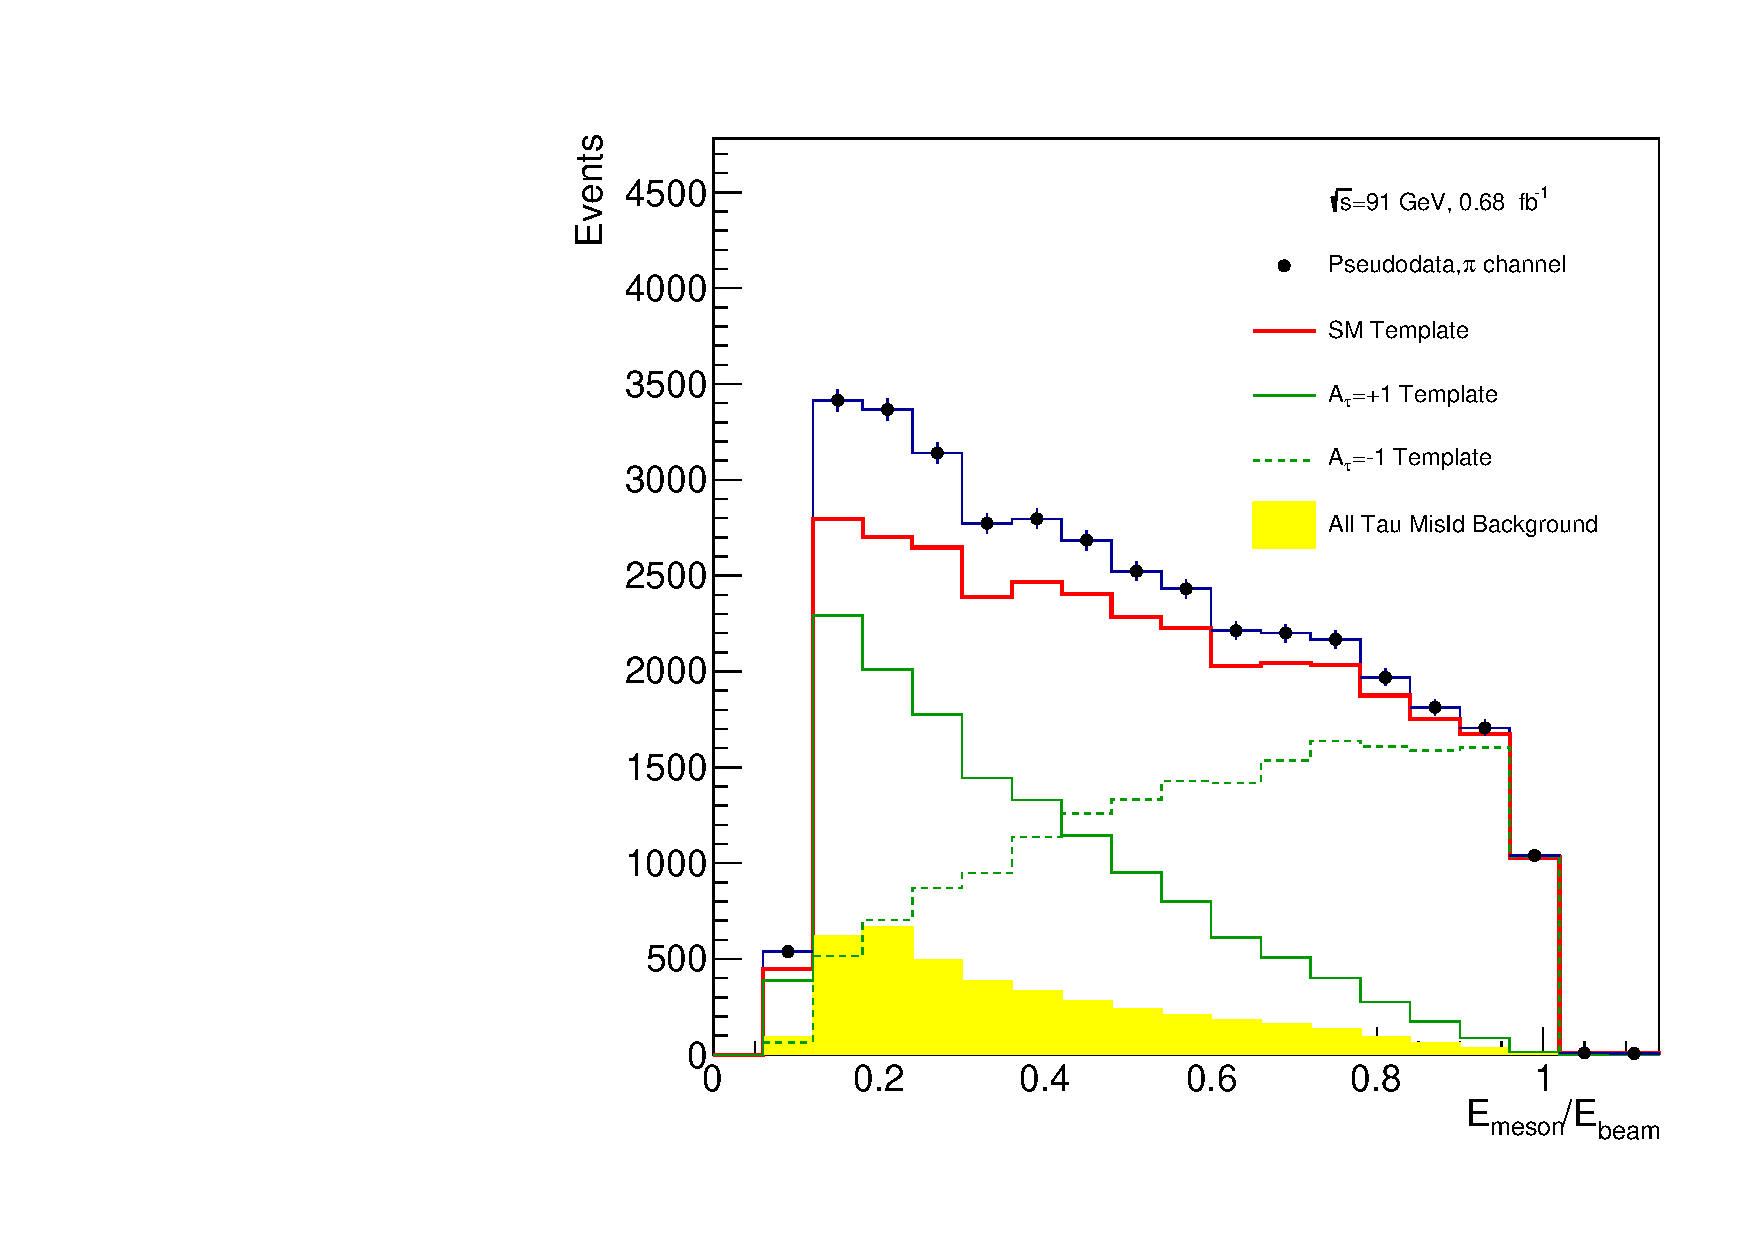
\includegraphics[width=0.48\textwidth]{DetectorRequirements/Figs/XPion.pdf} \\
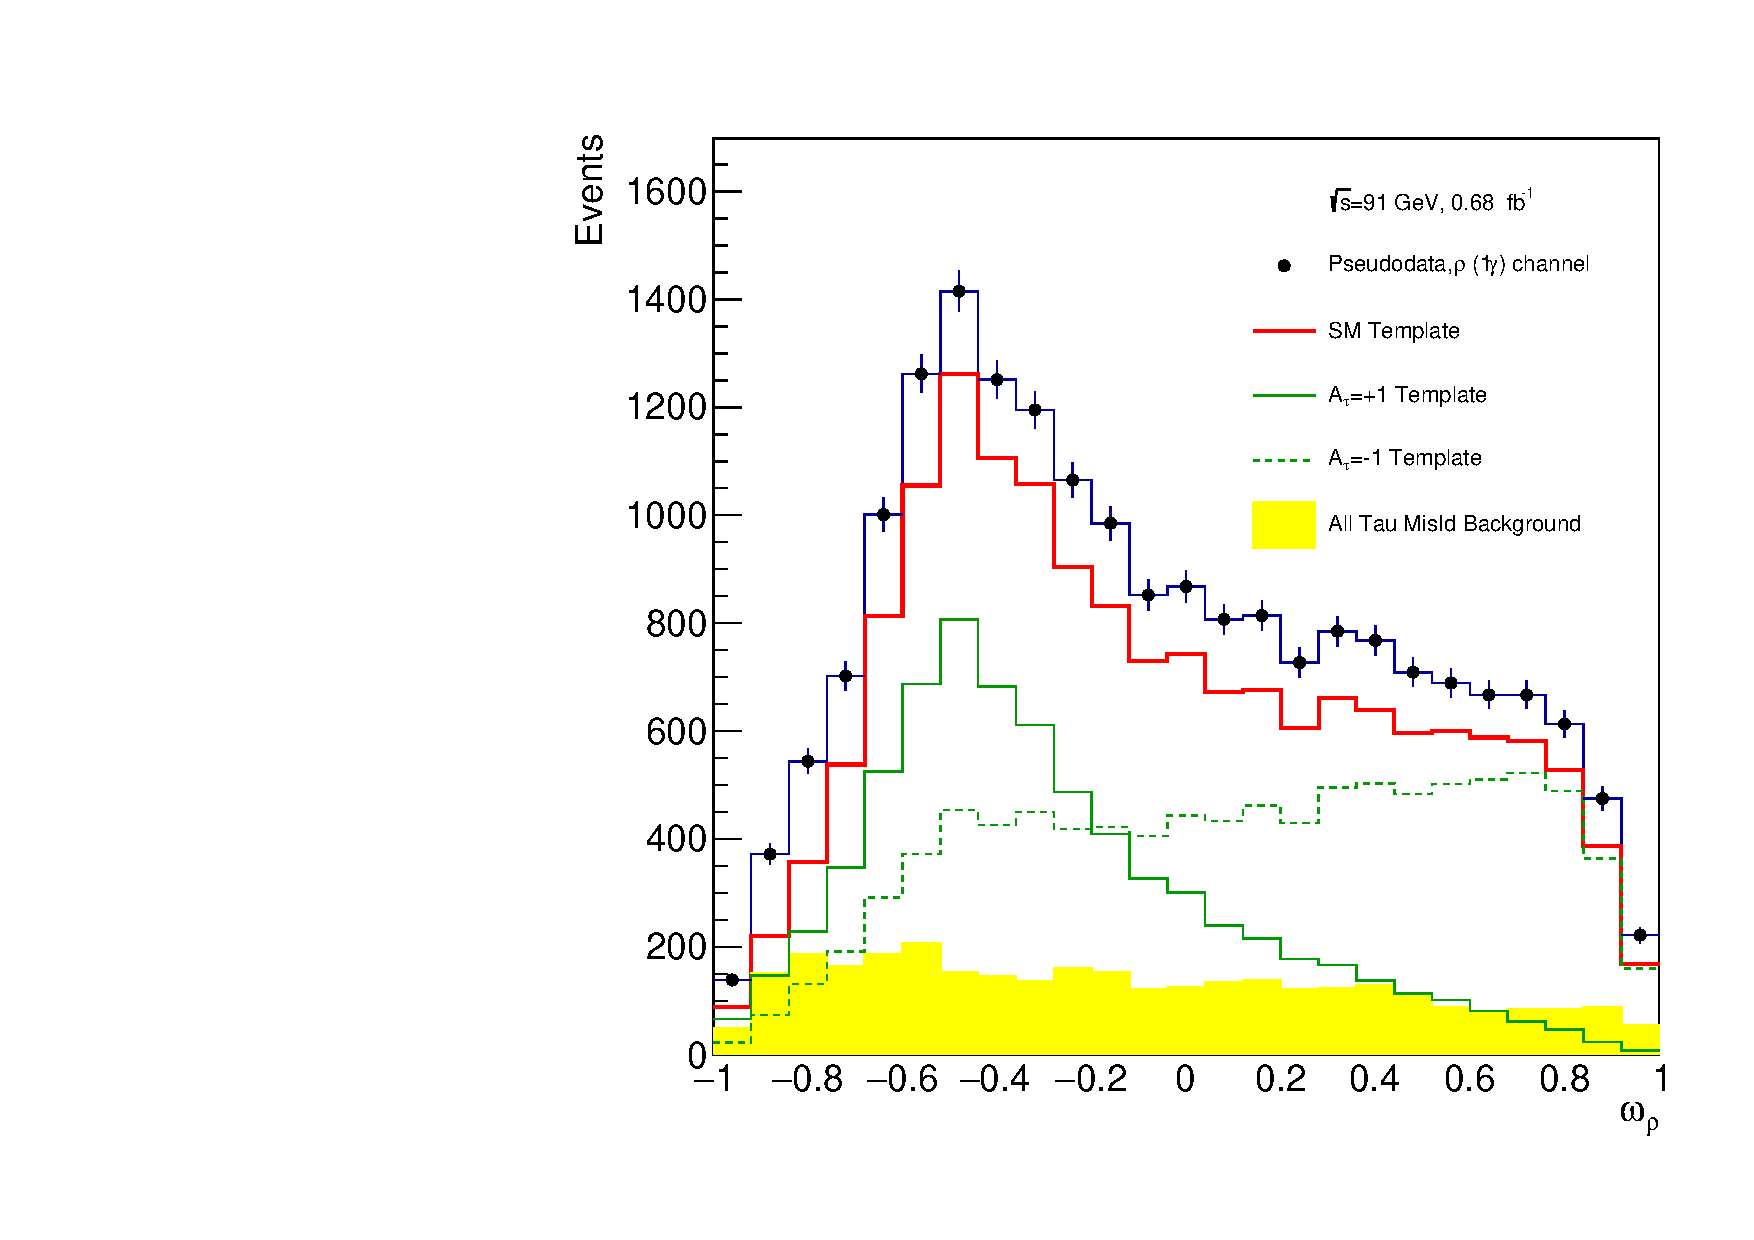
\includegraphics[width=0.48\textwidth]{DetectorRequirements/Figs/OmegaRhoMerged.pdf}
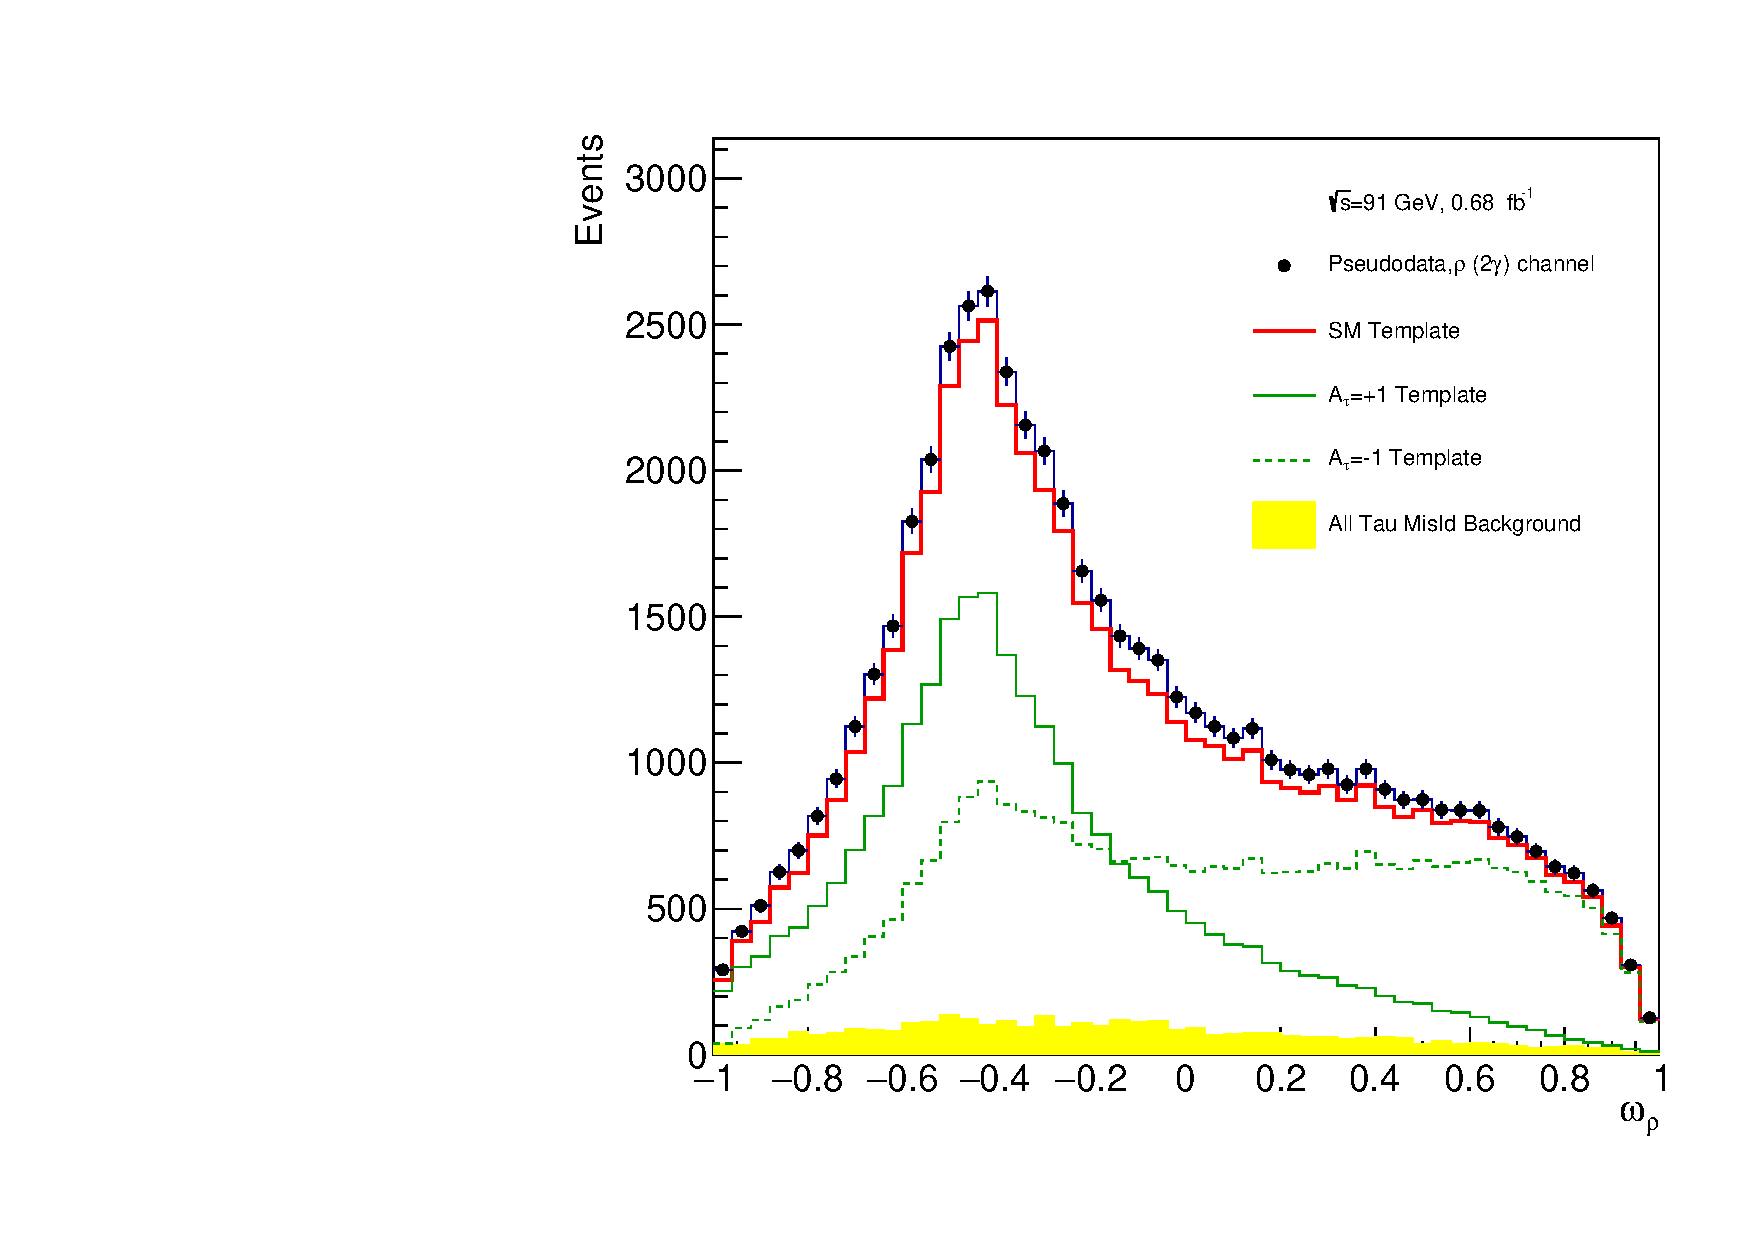
\includegraphics[width=0.48\textwidth]{DetectorRequirements/Figs/OmegaRhoResolved.pdf}    
\caption{Optimal variables used to extract the \PGt polarisation in three decay modes: 
\PGp (top), \PGr with one identified photon (bottom left), and \PGr with two identified photons (bottom right).}
\label{fig:fullsim_taupol}
\end{figure}

An analysis aiming to extract $\mathcal{A}_{\PGt}$ was performed using a log-likelihood fit of the optimal variable in the \PGr channel with two resolved photons. 
For an integrated luminosity of $17\,\text{ab}^{-1}$, corresponding to data collected by one FCC-ee experiment in a single year, 
the statistical uncertainty achieved is $7 \times 10^{-5}$. 
Future work includes refining the tau reconstruction algorithms, expanding the analysis to cover more decay channels and backgrounds, 
and performing a comprehensive extraction of the polarisation parameters across multiple $\cos\theta$ bins. 
In addition, focus will be placed on deriving explicit calorimeter requirements to reduce 
the dominant systematic uncertainties reflecting the \PGpz and fake photon identification efficiencies 
as close as possible to (or below) the statistical uncertainties.

\subsubsection{Summary of detector requirements}

The FCC-ee detectors are expected to perform precise measurements across a wide range of physics processes, 
requiring optimised designs. 
This summary provides a simplified overview of the key requirements, but it is important to recognise that these specifications often involve trade-offs, 
which should and will be studied in full simulation. 
For instance, incorporating a RICH or time-of-flight detector for particle identification may negatively impact the resolution of visible energy measurements. 
Identifying low-momentum muons effectively requires smaller detectors or a reduced magnetic field, 
which compromises the ability to accurately track high-momentum particles, impacting the overall physics programme. 
Finally, it should be noted that over-ambitious requirements could compromise the overall feasibility and the reliable operation of the detector systems. 
It is therefore of the utmost importance that the continued and creative effort to soften certain detector requirements with in-situ methods be consolidated and amplified.

\begin{table}[ht]
\renewcommand{\arraystretch}{2}
\centering
\caption{Summary of detector requirements.}
\label{tab:requirements}
\small
\begin{tabular}{lccc}
\toprule
& \textbf{Aggressive} & \textbf{Conservative} & \textbf{Comments} \\
\midrule
\textbf{Beampipe} & $X/X_0 < 0.5$\% & $X/X_0 < 1$\% & $\PB \to \PK^{\ast} \PGt \PGt$\\
\hline
\multirow{2}{*}{\textbf{Vertex}} & 
\makecell{$\sigma(d_0) = 3 \oplus 15\,/\,(p \, \sin^{3/2} \,\theta)$\,$\mu$m \\ $X/X_0 < 1$\%} & --  & \makecell{$\PB \to \PK^{\ast} \PGt \PGt$ \\ $R_{\PQc}$} \\
\cline{2-4}
& $\delta L = 5$\,ppm & -- & $\delta \tau_{\PGt} < 10$\,ppm\\
\hline
\multirow{2}{*}{\textbf{Tracking}} & 
\makecell{${\sigma_p}/{p} < 0.1$\% \\ for $\mathcal{O}$(50)\,GeV tracks} & 
\makecell{${\sigma_p}/{p} < 0.2$\% \\ for $\mathcal{O}$(50)\,GeV tracks} & 
\makecell{$\delta M_{\PH} = 4$\,\MeV \\ $\delta \Gamma_{\PZ} = 15$\,keV \\ $\PZ \to \PGt \PGm$} \\
\cline{2-4}
 & t.b.d.\ & $\sigma_\theta < 0.1$\,mrad &  $\delta \Gamma_{\PZ} (\text{BES}) < 10$\,keV \\
%
\hline
%
\multirow{3}{*}{\textbf{ECAL}} & 
${\sigma_E}/{E} = {3\%}/{\sqrt{E}}$ & ${\sigma_E}/{E} = {10\%}/{\sqrt{E}}$ & 
\makecell{$\PZ \to \PGne\PAGne$ coupling, \\ B physics, ALPs} \\
\cline{2-4} & 
\makecell{$\Delta x \times \Delta y =$ \\ $2 \times 2$\,mm$^2$} & 
\makecell{$\Delta x \times \Delta y =$ \\ $5 \times 5$\,mm$^2$} & 
\makecell{\PGt polarisation \\ boosted \PGpz decays \\ bremsstrahlung recovery }\\
\cline{2-4}
& \makecell{$\delta z = 100$\,\micron, \\ $\delta R_{\text{min}} = 10$\,\micron\ ($\theta = 20^\circ$)}
& \makecell{In-situ constraint with \\ dilepton/diphoton events} & 
\makecell{alignment tolerance for \\ $\delta \lumi = 10^{-5}$ with $\PGg\PGg$ events} \\ 
\hline
\multirow{2}{*}{\textbf{HCAL}} & 
${\sigma_E}/{E} = {30\%}/{\sqrt{E}}$ & ${\sigma_E}/{E} = {50\%}/{\sqrt{E}}$ & 
\makecell{$\PH \to \PQs\PAQs$, $\PQc\PAQc$, $\Pg\Pg$, invisible \\ HNLs} \\
\cline{2-4} & 
\makecell{$\Delta x \times \Delta y =$ \\ $2 \times 2$\,mm$^2$} & 
\makecell{$\Delta x \times \Delta y =$ \\ $20 \times 20$\,mm$^2$} & 
$\PH \to \PQs\PAQs$, $\PQc\PAQc$, $\Pg\Pg$\\
\hline
\textbf{Muons} & low momentum ($p < 1$\,GeV) ID & -- & $\PBs \to \PGn \PAGn$ \\
\hline
\textbf{Particle ID} & \makecell{3\,$\sigma$ $\PK/\PGp$ \\ $p < 40$\,GeV} & \makecell{3\,$\sigma$ $\PK/\PGp$ \\ $p < 30$\,GeV} & \makecell{$\PH \to \PQs\PAQs$ \\ $\PQb \to \PQs \PGn\PAGn$, \ldots}\\
\hline
\textbf{LumiCal} & \makecell{tolerance $\delta z = 100$\,\micron, $\delta R_{\text{min}} = 1$\,\micron \\ 
acceptance 50--100 mrad} & -- 
& \makecell{$\delta \lumi = 10^{-4}$ target \\ (Bhabha)} \\
\hline
\textbf{Acceptance} & 100\,mrad  & -- & \makecell{$\epem \to \PGg \PGg$ \\ $\epem \to \epem \PGtp \PGtm (\PQc\PAQc)$} \\
\bottomrule
\end{tabular}
\end{table}

An incomplete list of requirements is summarised in Table~\ref{tab:requirements}.
For physics channels involving charm, bottom, and tau production, the beam-pipe is required to have a minimal material budget, 
particularly critical for processes such as the $\PB \to \PK^\ast \PGt \PGt$ decay. 
The vertex detector must achieve a spatial resolution of 3\,$\mu$m or better and a material thickness below 1\% of a radiation length, 
to improve the precision of certain important measurements, 
such as the measurement of $R_{\PQc}$ at the \PZ pole or that of the branching fraction of the aforementioned $\PB \to \PK^\ast \PGt \PGt$ decay. 
The \PGt lifetime measurement requires the knowledge of the length scale of the vertex detector to be monitored with optical techniques with a precision of $\delta \tau_{\PGt} < 10$\,ppm. 
The momentum resolution in the tracking systems, $\sigma_p\,/\,p$, needs to be better than 0.2\% for ${\cal{O}}$(50)\,GeV tracks 
in order to achieve a precision of 4\,MeV on the Higgs boson mass. 
Achieving a precision of ${\cal{O}}$(10)\,keV on the \PZ width requires an exceptional track momentum resolution for such tracks, better than 0.1\%.
It also demands a precise knowledge of the BES, for which an angular tracking resolution $\sigma_\theta$ better than 0.1\,mrad is needed.
For flavour physics at the \PZ peak, where low momentum tracks are involved, 
a low mass gaseous tracker is advantageous since the momentum resolution is minimally affected by multiple scattering.
Having a highly-efficient and pure tracking from 100\,MeV to tens of GeV is of crucial importance to improve the dijet energy and mass resolution with particle-flow reconstruction.

Electromagnetic calorimetry with excellent energy resolution (few \%) is required to improve the precision 
on the $\PZ \to \PGne \PAGne$ coupling via the $\epem \to \PGne \PAGne \PGg$ process, 
on lepton flavour violating decays such as the $\PZ \to \PGm \Pe$ and $\PGt \to \PGm \PGg$ decays, 
on decays of heavy flavoured hadrons to photons or to \PGpz mesons, 
and on ALPs searches. 
The electromagnetic calorimeters must provide an energy resolution of $\sigma_E\,/\,E = 3\%\,/\,\sqrt{E}$
for aggressive scenarios and $10\%\,/\,\sqrt{E}$ for conservative ones, 
with spatial granularity between $2 \times 2$\,mm$^2$ and $5 \times 5$\,mm$^2$. 
High granularity is crucial for \PGt polarisation measurements, boosted \PGpz decays, and bremsstrahlung photon recovery. 
Additionally, alignment tolerances of $\delta z = 100$\,$\mu$m and $\delta R_\text{min} = 10$\,$\mu$m (measured at a 20$^\circ$ polar angle) 
are essential for a precise calibration of the acceptance or, equivalently, of the luminosity. 
The large dilepton and diphoton samples will be instrumental to ascertain in-situ the acceptance determination.

A good particle identification performance is required to achieve 3\,$\sigma$ $\PK/\PGp$ separation up to 30\,GeV 
and is essential for studying $\PH \to \PQs\PAQs$ decays, to study rare decays such as $\PQb \to \PQs \PGn \PAGn$, and, more generally, to maximise the FCC-ee flavour physics potential.

Hadron calorimeters with sufficient resolution and granularity are crucial for the success of the Higgs boson physics programme. 
In particular, the expected precision in the Higgs couplings to quarks and gluons is driven by the particle-flow global event reconstruction capabilities and the visible mass resolution. 
The hadron calorimeters must feature a stochastic term of less than 30\% in the aggressive scenario or less than 50\% in the more conservative scenarios. 
The transverse granularity should range from $2 \times 2$\,mm$^2$ to $20 \times 20$\,mm$^2$. 
The luminosity monitors must have a spatial tolerance of, at least, $\delta z = 100$\,$\mu$m and $\delta R_\text{min} = 1$\,$\mu$m, with an acceptance range of 50--100\,mrad. 
The detector must ensure optimal hermeticity. 
Requiring no gaps (and possibly a small overlap) between the LumiCal and the combined tracker plus calorimeter system 
sets the requirement for the tracker and calorimeter acceptance at 100\,mrad. 
Forward coverage is necessary for the detection and identification of photons produced in the $\epem \to \PGg \PGg$ process, 
which promises to provide an independent measurement of the luminosity. 
Processes involving the production of forward electrons, for example $\epem \to \epem \PGtp \PGtm (\PQc\PAQc)$ might also benefit from even more forward coverage.

Finally, the muon systems will be used mainly to identify muons, given that their momenta will be optimally measured by the tracking system at FCC-ee. 
They should provide excellent identification for pion rejection and standalone momentum measurement for long-lived particle searches. 

\subsection{Outlook}

Both software and analysis tools have matured during the Feasibility Study, 
and the common software framework (Chapter~\ref{sec:software}) was instrumental 
in developing a number of key physics case studies in view of extracting some of the necessary detector requirements. 
So far, most of the studies have been
performed with a fast simulation of the response of a few detector benchmarks, 
similar to those presented in the Conceptual Design Report. 
Variations around these baseline concepts were applied 
to quantify the generic sensitivity dependence of key observables on the detector performance. 
In the next phase of the study, 
more explicit requirements will be obtained with a (full) simulation, reconstruction, and analysis strategy, 
optimised to the specific capabilities of the considered hardware, 
when the current R\&D efforts start converging in concrete and definite detector proposals. 

Matching experimental systematic uncertainties to the FCC-ee statistical precision 
will remain a critical objective of the entire physics programme. 
This perspective constitutes a superb opportunity for detector designers. 
It also continuously generates new and creative ideas from the analysts to control uncertainties from the data themselves: 
past experience has shown that a careful analysis of systematic effects and corrections almost always
boils down to a statistical problem. 
This strategy will be generalised and will lead to a better precision for most observables, 
owing to the very large event samples expected at FCC-ee.   

With $6 \times 10^{12}$ \PZ and $3 \times 10^8$ \PW pairs, 
the leading challenge for the detector and analysis designs will continue to be the precision 
target with which the electroweak observables (Table~\ref{tab:EWPO}) can be measured.
%
Work on the hadronic, dilepton, and diphoton cross-section measurements has started, 
but much remains to be done, 
for example, to consolidate the in-situ acceptance determination method for lepton pairs 
and for the luminosity measurement with photon pairs and low-angle Bhabha scattering. 
The field of measurements at FCC-ee is huge, even when limited to the benchmark processes listed in
Ref.~\cite{SnowmassBenchmarkProcesses}. 
An even stronger connection between theorists and experimentalists will help streamlining and refining 
the list of observables and the parameter space to be explored. 
Clearly, the physics requirements will continue to be the driving factor in all efforts to design 
the most technologically-advanced (but also the most realistic) FCC-ee detector concepts, 
to ensure the full coverage of this challenging and promising physics programme.
